% 高一52_回民中学_9月月考.tex
%   —— 高一上数学“2026-2027 年回民中学高一上 9 月月考”（讲评版）
% 试卷版：xelatex 高一52_回民中学_9月月考.tex
% 答案版：xelatex "\def\isanswer{1}% 高一52_回民中学_9月月考.tex
%   —— 高一上数学“2026-2027 年回民中学高一上 9 月月考”（讲评版）
% 试卷版：xelatex 高一52_回民中学_9月月考.tex
% 答案版：xelatex "\def\isanswer{1}% 高一52_回民中学_9月月考.tex
%   —— 高一上数学“2026-2027 年回民中学高一上 9 月月考”（讲评版）
% 试卷版：xelatex 高一52_回民中学_9月月考.tex
% 答案版：xelatex "\def\isanswer{1}% 高一52_回民中学_9月月考.tex
%   —— 高一上数学“2026-2027 年回民中学高一上 9 月月考”（讲评版）
% 试卷版：xelatex 高一52_回民中学_9月月考.tex
% 答案版：xelatex "\def\isanswer{1}\input{高一52_回民中学_9月月考.tex}"
% 紧凑版：xelatex "\def\iscompact{1}\input{高一52_回民中学_9月月考.tex}"
%
% 原始材料：微信公众号“魔都数学加油站”文章，作者破晓，连载“27学年高一52”；
% 原文标题“27学年高一52——2026-2027年上海市回民中学高一上9月月考”；
% 原文链接：https://mp.weixin.qq.com/s/ndjyozrRQCLl4ba3J8uR7g。
% 该页面用 JS 渲染，未见明确发布日期；页面内时间戳约为 2026-10-06 21:19／21:38，本稿以该时刻记可得日期。
% 正文为 8 张 PNG 页：第 01—07 页 4762×6735，第 08 页 2560×3620（**同一篇各页分辨率不同**），
% 均按页序读取。8 页全为试卷正文页（卷首标题在第 1 页页顶，卷末解答题第 21 题解析止于第 8 页），
% 无封面页、目录页、二维码或宣传页。粉色斜排“魔都数学加油站”为卷面水印，与公众号页脚一并未录入。
%
% 卷首标题：照卷面印作“2026--2027 年回民中学高一上 9 月月考”（公众号标题中的“上海市”
% 卷面标题行没有，本稿照卷面），年份区间按全稿惯例排 en dash。原卷只有一行标题、无副标题。
%
% 篇幅与题号：原卷自第 3 题起编号（第 1、2 题不在本卷内）。填空题 3—12（10 题）、
% 选择题 13—16（4 题）、解答题 17—21（5 题），共 19 题。本稿沿用原节与原题号，
% 只改排为全稿统一的大节样式（原卷小节标题为“一、填空题”“二、选择题”“三、解答题”）。
%
% 讲评版：原卷每题下直接印【答案】或【解析】。**只印【答案】的 1 题**（第 3 题），本稿只给 \ans{}；
% **第 14 题没有任何【答案】/【解析】段**，答案“D”直接印在题干括号内（“应假设(  D  )”），
% 本稿按 高一37 第 13 题的成例把括号留空、答案另提为 \ans{$D$}；
% 其余 17 题都只印【解析】，按全稿口径这类题不另提 \ans{}——其中选择题第 13、15、16 题的结论
% 写在解析末句（“故选 A／A／B”），亦照录在解析内。
%
% 副标题：原卷未印副标题。本稿按“知识模块”口径标作“集合与常用逻辑用语、不等式”：
% 19 题中集合与常用逻辑用语 10 题（集合类 7 题——第 3、4、5、9、12、16、21 题；
% 逻辑类 3 题——第 6、14、15 题），不等式 9 题（含等式性质与一元二次方程：第 7、8、10、11、
% 13、17、18、19、20 题），两类均远超三分之一，故并标。口径同 高一46、高一47、高一48、高一51。
%
% 与原卷的排版差异：
%   ① 原卷每题下直接印【答案】/【解析】，本稿按全稿惯例将答案与解析置于答案版，试卷版保持干净；
%      第 14 题印在题干括号内的答案“D”同样移入 \ans{}，见上；
%   ② 原卷未印副标题，本稿按“知识模块”口径补出；
%   ③ 原卷填空横线约两个字宽，本稿按全稿惯例统一排 \blankline[4.4em]；
%      选择题的作答括号原卷排半角“(    )”，本稿按全稿惯例排 \mbox{（\quad）}；
%   ④ 原卷实数集、自然数集排斜体/粗体 $R$、$\mathbf{R}$、$N$，本稿按全稿惯例改用 $\R$、$\N$；
%      空集记号统一为 \varnothing；
%   ⑤ 第 8 题题干与解析两处“两个实数分别为 $x_1$、$x_2$”原卷即用顿号，第 10、13 题等处
%      原卷在数学式内用半角逗号（如 $x_1,x_2$、$a,b,c\in R$），两份均照录未强改；
%      句末句点按全稿惯例排西文句点，句中句点（第 9、12、15、21 题）照原卷排全角“．”；
%   ⑥ 第 17、20 题原卷把子问标号“（1）”排在该题题号同一行，本稿照原卷仍排同一行（同 高一34 的
%      做法）；第 18、19、21 题的子问原卷各自另起一行，本稿按全稿惯例用 enumerate 的 (1)(2)(3)；
%      解析中的子问标号一律用 \stepm{(1)}{…}；
%   ⑦ 第 16 题的韦恩图原卷排在题干与选项右侧的浮动位置，本稿居中排在题干之后、选项之前，
%      并加 \needvspace 整块推走（守卫写在 \item 之前）；图自原图第 4 页裁切（trim），不另存图片文件；
%   ⑧ 每道解答题原卷未留作答空白，本稿按全稿惯例加 \ansspace。
%
% 原卷笔误/存疑（均照录未改，正文对应处另有 % 注）：
%   1. 第 8 题题干与解析首行两处均作“两个实数分别为 $x_1$、$x_2$”，按文意应为“两个实数**根**”
%      （疑脱“根”字，第 10 题同位置作“两个实根分别是”）；
%   2. 第 4 题解析“满足条件的 $A$ 的个数为集合 $\{0,1,3\}$ 的真子集，即 7 个”，
%      “个数为……真子集”表述不严（应为“……的真子集的个数”）；$\{0,1,3\}$ 的真子集 7 个，结论无误；
%   3. 第 6 题解析第 2 行“当 $a=10,b=0.2$ 时，$a+b>2$，且 $ab>1$，所以 $a>1$，且 $b>1$ 不成立”
%      ——此处是举反例，“所以”按文意应为“但”（$a=10,b=0.2$ 与“$a>1$ 且 $b>1$”不成立之间是转折，
%      非因果）；
%   4. 第 19 题 (1) 解析末行“综上，$a>b$ 是 $\dfrac1a<\dfrac1b$ 的充要条件。”用全角句号“。”，
%      全卷其余各题末句均用“．”，体例不一，照录；
%   5. 第 20 题第 (1) 问解析先按 $m>2$、$m=2$、$m<2$ 三种情况各给出解集，末三行又“综上”重述一遍，
%      与原卷一致（内容重复，非笔误）；
%   6. 第 18 题题干第 (2) 问“若 $p,q$ 两命题一真一假”，正文照录原卷所用半角逗号（未改顿号）。
%
% 插图：1 张，自原图裁切（无 \begin{tikzpicture} 重排）：
%   · 第 16 题题干韦恩图（全集 $U$ 矩形内两相交椭圆 $A$、$B$，灰色为阴影部分）
%     ——原图第 04 页，原卷排于题干与选项右侧。
%     裁框：x 3594–4558、y 2826–3317（即矩形外框，四周各留 4px），
%     trim=3590bp 3414bp 200bp 2822bp（左／下／右／上），页宽 4762、页高 6735。
%
\documentclass[a4paper,11pt]{article}
\usepackage{common}

\begin{document}

\examtitlest[3]{2026--2027 年回民中学高一上 9 月月考}{集合与常用逻辑用语、不等式}

\bigsec{一、填空题}

\begin{enumerate}
\setcounter{enumi}{2}

\item 用列举法写出下列集合 $\{(x,y)\mid x+y=2,x\in\N,y\in\N\}=$\blankline[4.4em].

\ifanswer
\ans{$\{(0,2),(1,1),(2,0)\}$}
\fi

\item 设集合 $A$ 满足 $\{-1,2\}\sub A\subset\{-1,0,1,2,3\}$，则满足条件的 $A$ 有\blankline[4.4em]个.

\ifanswer
\solbegin
\step{满足条件的 $A$ 的个数为集合 $\{0,1,3\}$ 的真子集，即 $7$ 个.}
\solend
\fi

\item 已知集合 $A=\{2,(a+1)^2,a^2+2\}$，且 $1\in A$，则实数 $a$ 的值为\blankline[4.4em].

\ifanswer
\solbegin
\step{因为 $1\in A$，而 $a^2+2\geqslant2$，所以 $(a+1)^2=1$，解得 $a=0$ 或 $a=-2$，}
\step{$a=0$ 时，$a^2+2=2$，不合题意，$a=-2$ 时，$a^2+2=6$，满足题意，}
\step{所以 $a=-2$.}
\solend
\fi

\item 已知 $a,b$ 是实数，则“$a>1$，且 $b>1$”是“$a+b>2$，且 $ab>1$”的\blankline[4.4em]条件.

\ifanswer
\solbegin
\step{$a,b$ 是实数，则“$a>1$，且 $b>1$”$\Rightarrow$“$a+b>2$，且 $ab>1$”正确，}
% 原卷如此，照录未改（第 6 题解析此处作“所以 $a>1$，且 $b>1$ 不成立”，按文意为转折，
% 见文件头“原卷笔误/存疑”第 3 条）
\step{当 $a=10,b=0.2$ 时，$a+b>2$，且 $ab>1$，所以 $a>1$，且 $b>1$ 不成立，}
\step{即前者是推出后者，后者推不出前者，}
\step{所以“$a>1$，且 $b>1$”是“$a+b>2$，且 $ab>1$”的充分而不必要条件.}
\solend
\fi

\item 已知等式 $2x^2-3x-1=a(x-1)^2+b(x-1)+c$ 恒成立，其中 $a,b,c$ 为常数，则 $a+b-c=$\blankline[4.4em].

\ifanswer
\solbegin
\step{将等式右侧展开整理得 $a(x-1)^2+b(x-1)+c=ax^2+(-2a+b)x+(a-b+c)$，}
\step{左右两边多项式恒等，对应次数的系数必须相等：}
\step{则 $a=2,-2a+b=-3$，代入 $a=2$ 得 $b=1$，$a-b+c=-1$，}
\step{代入 $a=2,b=1$ 得 $c=-2$，得 $a+b-c=2+1-(-2)=5$.}
\solend
\fi

% 原卷如此，照录未改（第 8 题题干与解析首行两处“两个实数分别为”疑脱“根”字，
% 见文件头“原卷笔误/存疑”第 1 条）
\item 若关于 $x$ 的二次方程 $x^2+mx+4m^2-3=0$ 的两个实数分别为 $x_1$、$x_2$，且满足 $x_1+x_2=x_1x_2$，则实数 $m$ 的值为\blankline[4.4em].

\ifanswer
\solbegin
% 原卷如此，照录未改（此处“两个实数分别为”同题干，疑脱“根”字）
\step{二次方程 $x^2+mx+4m^2-3=0$ 的两个实数分别为 $x_1$、$x_2$，}
\step{则有 $\Delta=m^2-4(4m^2-3)\geqslant0$，变形得 $m^2\leqslant\dfrac45$，}
\step{则 $x_1+x_2=-m$，$x_1x_2=(4m^2-3)$，}
\step{若 $x_1+x_2=x_1x_2$，则有 $-m=4m^2-3$，解得 $m=-1$ 或 $\dfrac34$，}
\step{又 $m^2\leqslant\dfrac45$，则 $m=\dfrac34$.}
\solend
\fi

\item 设集合 $A=\{x\mid x^2=1\}$，$B=\{x\mid ax=1\}$．若 $A\cap B=B$，则实数 $a$ 的值为\blankline[4.4em].

\ifanswer
\solbegin
\step{集合 $A=\{x\mid x^2=1\}=\{-1,1\}$，$B=\{x\mid ax=1\}$，$A\cap B=B$，所以 $B\sub A$，}
\step{当 $a=0$ 时，$B=\varnothing$，成立；}
\step{当 $a\neq0$ 时，$B=\left\{\dfrac1a\right\}$，则 $\dfrac1a=-1$ 或 $\dfrac1a=1$，解得 $a=-1$ 或 $a=1$，}
\step{所以实数 $a$ 的值为 $0$ 或 $1$ 或 $-1$.}
\solend
\fi

\item 已知关于 $x$ 的一元二次方程 $x^2+3x-3=0$ 的两个实根分别是 $x_1,x_2$，则以 $-\dfrac1{x_1},-\dfrac1{x_2}$ 为根且二次项系数是 $1$ 的一元二次方程为\blankline[4.4em].

\ifanswer
\solbegin
\step{因为 $x_1,x_2$ 是一元二次方程 $x^2+3x-3=0$ 的两个实根，}
\step{所以 $x_1+x_2=-3,x_1x_2=-3$，}
\step{所以 $-\dfrac1{x_1}+\left(-\dfrac1{x_2}\right)=-\dfrac{x_1+x_2}{x_1x_2}=-1$，$-\dfrac1{x_1}\cdot\left(-\dfrac1{x_2}\right)=\dfrac1{x_1x_2}=-\dfrac13$，}
\step{所以一元二次方程为 $x^2+x-\dfrac13=0$.}
\solend
\fi

\item 若关于 $x$ 的不等式 $(a-2)x^2+2(a-2)x-4<0$ 的解集是 $\R$，则实数 $a$ 的取值范围是\blankline[4.4em].

\ifanswer
\solbegin
\step{当 $a=2$ 时，不等式化为 $-4<0$ 对于任意实数 $x$ 都成立，因此 $a=2$ 满足题意；}
\step{当 $a\neq2$ 时，要使关于 $x$ 的不等式 $(a-2)x^2+2(a-2)x-4<0$ 的解集为 $\R$，}
\step{则 $\begin{cases}a-2<0\\ \Delta=4(a-2)^2+16(a-2)<0\end{cases}$，解得 $-2<a<2$．}
\step{综上，$a$ 的取值范围为 $(-2,2]$．}
\solend
\fi

\item 设非空集合 $A$、$B$，定义 $A\times B=\{x\mid x\in(A\cup B),x\notin(A\cap B)\}$．已知 $A=\{x\mid0\leqslant x\leqslant2\}$，$B=\{y\mid y\geqslant0\}$，则 $A\times B=$\blankline[4.4em].

\ifanswer
\solbegin
\step{由于 $A=\{x\mid0\leqslant x\leqslant2\}$，$B=\{y\mid y\geqslant0\}=\{x\mid x\geqslant0\}$，}
\step{所以 $A\cup B=\{x\mid x\geqslant0\}$，$A\cap B=\{x\mid0\leqslant x\leqslant2\}$，故 $A\times B=\{x\mid x>2\}$．}
\solend
\fi

\end{enumerate}

\bigsec{二、选择题}

\begin{enumerate}
\setcounter{enumi}{12}

\item 已知 $a,b,c\in\R$ 且 $a>b$，则下列不等式一定成立的是\mbox{（\quad）}

\keepwithprev
A. $\dfrac{a}{c^2+1}>\dfrac{b}{c^2+1}$\qquad B. $\dfrac1a<\dfrac1b$

C. $ac>bc$\qquad D. $a^2>b^2$

\ifanswer
\solbegin
\step{对于 A：因为 $c^2+1>0$ 恒成立，且 $a>b$，所以 $\dfrac{a}{c^2+1}>\dfrac{b}{c^2+1}$ 一定成立，}
\step{所以 A 正确；}
\step{对于 B：当 $a=1,b=-1$ 时，满足 $a>b$，此时 $\dfrac1a=1>\dfrac1b=-1$，所以 B 错误；}
\step{对于 C：当 $c<0$ 时，由 $a>b$，得 $ac<bc$，所以 C 错误；}
\step{对于 D：当 $a=1,b=-2$ 时，满足 $a>b$，此时 $a^2=1<b^2=4$，所以 D 错误；}
\step{故选 $A$．}
\solend
\fi

% 注：本题的答案“D”原卷直接印在题干末尾的括号内（“应假设(  D  )”），且没有单独的
%     【答案】/【解析】段，本稿按 高一37 第 13 题的成例把括号留空、另提为 \ans{}，
%     见文件头“与原卷的排版差异”①。
\item 用反证法证明：“已知 $x,y\in\R$,$x^2+y^2=0$，求证：$x=y=0$”时，应假设\mbox{（\quad）}

\keepwithprev
A. 已知 $x^2+y^2=0,x\neq0$ 且 $y\neq0$\qquad B. $x\neq0$ 且 $y\neq0$

C. 已知 $x^2+y^2=0,x\neq0$ 或 $y\neq0$\qquad D. $x\neq0$ 或 $y\neq0$

\ans{$D$}

\item 《齐民要术》是中国杰出农学家贾思勰（xié）所著的一部综合性农学著作，也是中国现存最早的一部完整的农书，被誉为“中国古代农业百科全书”．书中有一句为“顺天时，量地利，则用力少而成功多”．大意是说根据规律办事，就可以用较少的力收获更多的成功．则“顺天时，量地利”是“用力少而成功多”的\mbox{（\quad）}

\keepwithprev
A. 充分条件\qquad B. 必要条件

C. 充要条件\qquad D. 既非充分也非必要条件

\ifanswer
\solbegin
\step{如果顺应天时地利的万物规律，就能花费较少的力取得更多成功，充分性成立；}
\step{而用力少而成功多的前提不一定是顺天时，量地利，比如某种果实产量高，}
\step{有可能是播种方式或者灌溉频率等人为因素，必要性不成立；}
\step{则“顺天时，量地利”是“用力少而成功多”的充分不必要条件．故选 $A$．}
\solend
\fi

\needvspace{13\baselineskip}

\item 如图，已知全集 $U=\R$，集合 $A=\{x\mid(2x-3)\cdot(x+1)\leqslant0\}$，$B=\{x\mid x>0\}$，则图中阴影部分表示的集合为\mbox{（\quad）}

\begin{center}
% 原图第 4 页题干韦恩图直接裁取（原卷排于题干与选项右侧）。
% 裁框取矩形外框 x 3590–4558、y 2822–3321，再向外各留 4px（即 x 3586–4562、y 2818–3325），
% trim=左 3586bp／下 3410bp／右 196bp／上 2818bp（页宽 4762、页高 6735）。
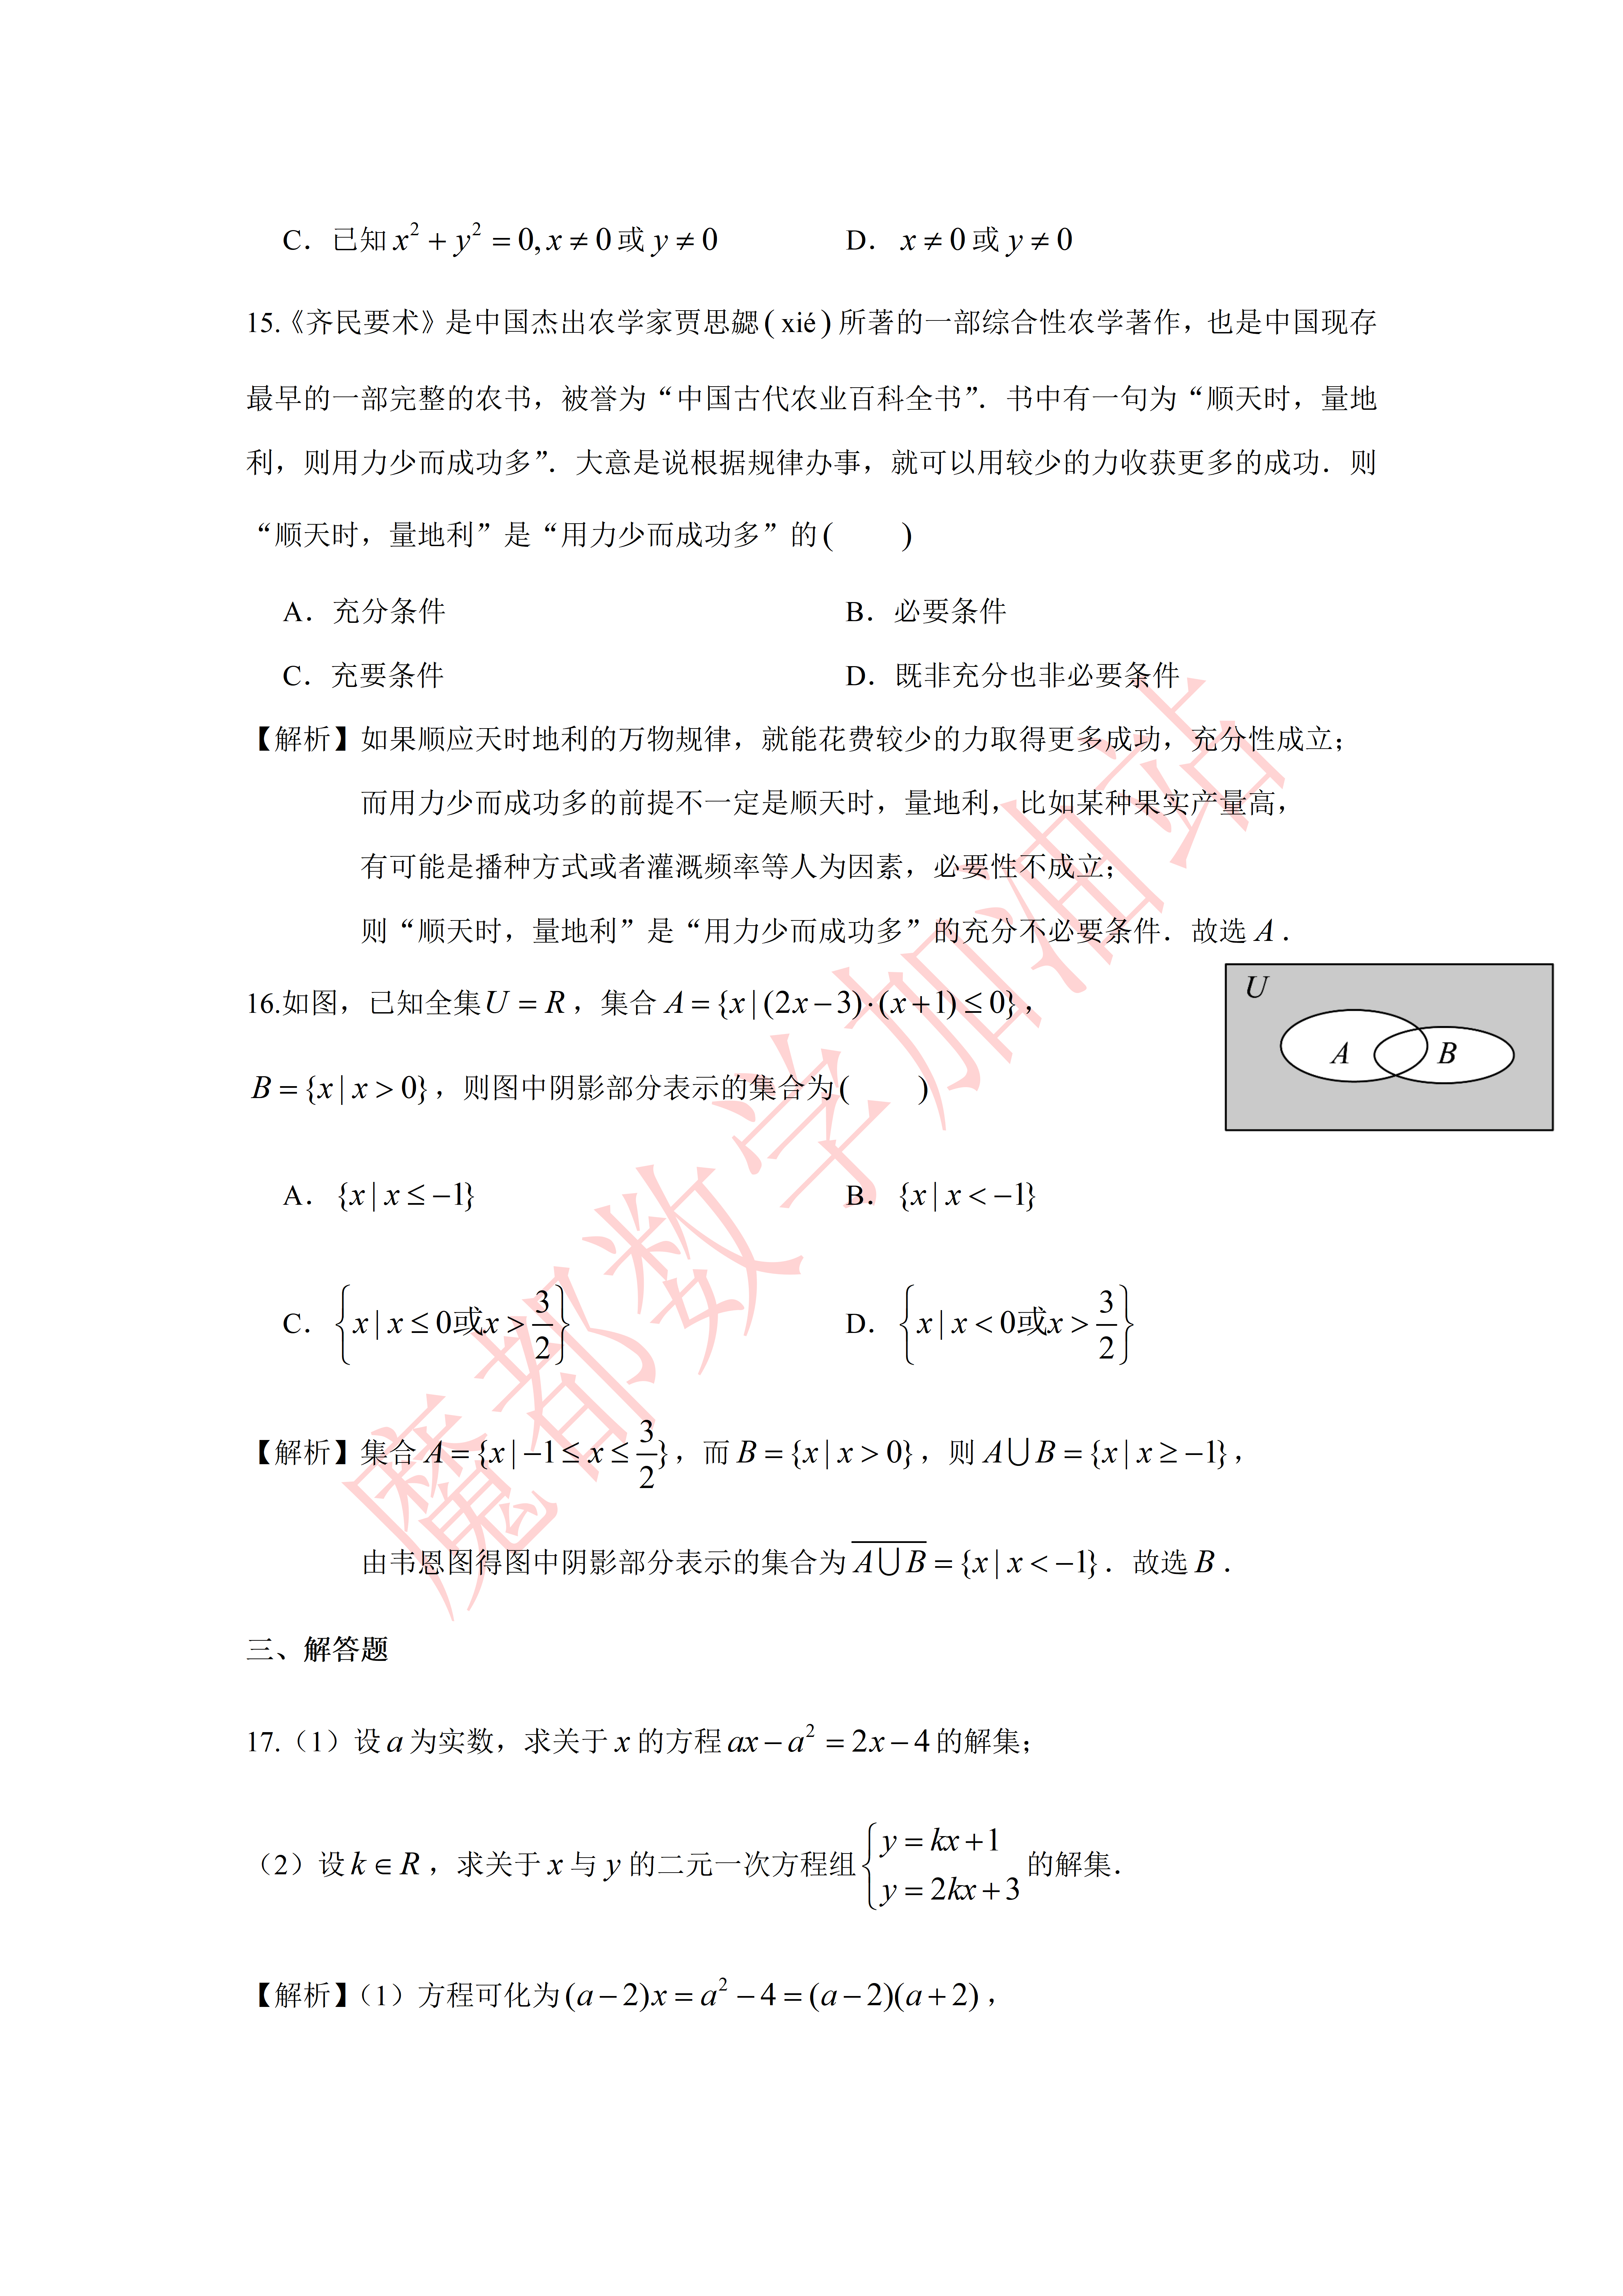
\includegraphics[width=.34\linewidth,trim=3586bp 3410bp 196bp 2818bp,clip]{../原图/高一52_回民中学_9月月考/04.png}
\end{center}

\keepwithprev
A. $\{x\mid x\leqslant-1\}$\qquad B. $\{x\mid x<-1\}$

C. $\left\{x\mid x\leqslant0\text{ 或 }x>\dfrac32\right\}$\qquad D. $\left\{x\mid x<0\text{ 或 }x>\dfrac32\right\}$

\ifanswer
\solbegin
\step{集合 $A=\left\{x\mid-1\leqslant x\leqslant\dfrac32\right\}$，而 $B=\{x\mid x>0\}$，则 $A\cup B=\{x\mid x\geqslant-1\}$，}
\step{由韦恩图得图中阴影部分表示的集合为 $\overline{A\cup B}=\{x\mid x<-1\}$．故选 $B$．}
\solend
\fi

\end{enumerate}

\bigsec{三、解答题}

\begin{enumerate}
\setcounter{enumi}{16}

\item （1）设 $a$ 为实数，求关于 $x$ 的方程 $ax-a^2=2x-4$ 的解集；

（2）设 $k\in\R$，求关于 $x$ 与 $y$ 的二元一次方程组 $\begin{cases}y=kx+1\\y=2kx+3\end{cases}$ 的解集．

\ifanswer
\solbegin
\stepm{(1)}{方程可化为 $(a-2)x=a^2-4=(a-2)(a+2)$，}
\step{当 $a\neq2$ 时，方程的解为 $x=\dfrac{(a-2)(a+2)}{a-2}=a+2$，则解集为 $\{a+2\}$；}
\step{当 $a=2$ 时，方程为 $2x-4=2x-4$，对 $x$ 取一切实数均成立，}
\step{所以解集为 $\R$；}
\stepm{(2)}{$\begin{cases}y=kx+1\\y=2kx+3\end{cases}$，则 $kx+1=2kx+3,kx=-2$，}
\step{当 $k=0$ 时，等式不成立，无解；当 $k\neq0$ 时，$x=-\dfrac2k,y=-1$；}
\step{综上所述，当 $k=0$ 时，解集为 $\varnothing$；当 $k\neq0$ 时，解集为 $\left\{\left(-\dfrac2k,-1\right)\right\}$．}
\solend
\fi

\ansspace[6]

\item 已知命题 $p$：方程 $x^2+6x+m-1=0$ 有两个不等的负根；命题 $q$：方程 $9x^2+6x+m-2=0$ 无实根．

\begin{enumerate}[label=(\arabic*)]
\item 若 $p$ 为真命题，求实数 $m$ 的取值范围；
\item 若 $p,q$ 两命题一真一假，求实数 $m$ 的取值范围．
\end{enumerate}

\ifanswer
\solbegin
\stepm{(1)}{设方程 $x^2+6x+m-1=0$ 两根为 $x_1,x_2$，}
\step{则 $\begin{cases}\Delta>0\\ x_1+x_2<0\\ x_1x_2>0\end{cases}\Rightarrow\begin{cases}36-4(m-1)>0\\ -6<0\\ m-1>0\end{cases}\Rightarrow1<m<10$；}
\stepm{(2)}{若命题 $q$ 为真命题，则 $36-36(m-2)<0\Rightarrow m>3$，}
\step{从而当命题 $q$ 为假命题时，$m\leqslant3$；}
\step{又由（1）得 $p$ 为假命题时，$m\leqslant1$ 或 $m\geqslant10$；}
\step{则当 $p$ 为真命题，$q$ 为假命题时，得 $\begin{cases}1<m<10\\ m\leqslant3\end{cases}\Rightarrow1<m\leqslant3$；}
\step{当 $q$ 为真命题，$p$ 为假命题时，得 $\begin{cases}m\leqslant1\text{ 或 }m\geqslant10\\ m>3\end{cases}\Rightarrow m\geqslant10$；}
\step{综上，当 $p,q$ 两命题一真一假时，$1<m\leqslant3$ 或 $m\geqslant10$.}
\solend
\fi

\ansspace[6]

\item 证明下列两个命题：

\begin{enumerate}[label=(\arabic*)]
\item 设 $ab>0$，求证：$a>b$ 是 $\dfrac1a<\dfrac1b$ 的充要条件．
\item 已知 $a,b$ 为正数，$n$ 为正整数，求证：如果 $a^n>b^n$，那么 $a>b$．
\end{enumerate}

\ifanswer
\solbegin
\stepm{(1)}{先证充分性：因为 $ab>0$ 且 $a>b$，故 $a-b>0$，从而 $\dfrac{a-b}{ab}>0$，}
\step{即 $\dfrac1b-\dfrac1a>0$，即 $\dfrac1a<\dfrac1b$；}
\step{再证必要性：若 $\dfrac1a<\dfrac1b$，则 $\dfrac1a-\dfrac1b=\dfrac{b-a}{ab}<0$，}
\step{又因为 $ab>0$，所以 $b-a<0$，即 $a>b$．}
% 原卷如此，照录未改（第 19 题(1)此句末用全角句号“。”，全卷其余各题末句用“．”，
% 见文件头“原卷笔误/存疑”第 4 条）
\step{综上，$a>b$ 是 $\dfrac1a<\dfrac1b$ 的充要条件。}
\stepm{(2)}{令 $f(x)=x^n,n\in\N^*$，则由幂函数的性质得 $f(x)$ 在第一象限是严格增的，}
\step{而 $a^n>b^n$ 即意味着 $f(a)>f(b)$，且 $a,b$ 为正数，从而 $a>b$．}
\solend
\fi

\ansspace[8]

\item （1）求关于 $x$ 的不等式 $(m-2)x>1-m$ 的解集；

（2）求关于 $x$ 的不等式 $x^2-(a+1)x+a\leqslant0$ 的解集．

\ifanswer
\solbegin
\stepm{(1)}{由不等式 $(m-2)x>1-m$，}
\step{当 $m-2>0$ 时，即 $m>2$ 时，解得 $x>\dfrac{1-m}{m-2}$，}
\step{所以不等式的解集为 $\left(\dfrac{1-m}{m-2},+\infty\right)$；}
\step{当 $m-2=0$ 时，即 $m=2$ 时，不等式即为 $0>-1$ 恒成立，}
\step{即不等式的解集为 $\R$；}
\step{当 $m-2<0$ 时，即 $m<2$ 时，解得 $x<\dfrac{1-m}{m-2}$，}
\step{所以不等式的解集为 $\left(-\infty,\dfrac{1-m}{m-2}\right)$；}
\step{综上，当 $m>2$ 时，解集为 $\left(\dfrac{1-m}{m-2},+\infty\right)$；}
\step{当 $m=2$ 时，解集为 $\R$；}
\step{当 $m<2$ 时，解集为 $\left(-\infty,\dfrac{1-m}{m-2}\right)$．}
\stepm{(2)}{由不等式 $x^2-(a+1)x+a\leqslant0$，可化为 $(x-a)(x-1)\leqslant0$，}
\step{当 $a>1$ 时，解得 $1\leqslant x\leqslant a$，即不等式的解集为 $[1,a]$；}
\step{当 $a=1$ 时，不等式即为 $(x-1)^2\leqslant0$，解得 $x=1$，即不等式的解集为 $\{1\}$；}
\step{当 $a<1$ 时，解得 $a\leqslant x\leqslant1$，即不等式的解集为 $[a,1]$，}
\step{综上，当 $a>1$ 时，解集为 $[1,a]$；}
\step{当 $a=1$ 时，解集为 $\{1\}$；}
\step{当 $a<1$ 时，解集为 $[a,1]$．}
\solend
\fi

\ansspace[10]

\item 已知集合 $A=\{x\mid(x+2)(5-x)\geqslant0\}$，若集合 $B$ 满足 $A\cap B=\varnothing,A\cup B=[-2,7)$．

\begin{enumerate}[label=(\arabic*)]
\item 用区间表示集合 $B$；
\item 若集合 $B$ 是不等式 $-x^2+bx+c>0$ 的解集，求实数 $b,c$ 的值；
\item 已知全集为 $\R$，若关于 $x$ 的不等式 $-1<x-a\leqslant2$ 的解集为 $M$，且“$x\in\overline A$”是“$x\in M$”的必要非充分条件，求实数 $a$ 的取值范围．
\end{enumerate}

\ifanswer
\solbegin
\stepm{(1)}{由题意得 $(x+2)(5-x)\geqslant0\Leftrightarrow(x+2)(x-5)\leqslant0\Rightarrow-2\leqslant x\leqslant5$，}
\step{则 $A=[-2,5]$，又 $A\cap B=\varnothing,A\cup B=[-2,7)$，则 $B=(5,7)$；}
\stepm{(2)}{$-x^2+bx+c>0\Leftrightarrow x^2-bx-c<0$，则 $x^2-bx-c=0$ 两根为 $5,7$，}
\step{则由韦达定理得 $b=12,-c=35\Rightarrow c=-35$；}
\stepm{(3)}{由题意得 $M=(a-1,a+2],\overline A=(-\infty,-2)\cup(5,+\infty)$，}
\step{且“$x\in\overline A$”是“$x\in M$”的必要非充分条件，则 $M$ 是 $\overline A$ 的真子集，}
\step{从而 $a+2<-2$ 或 $a-1\geqslant5$，解得 $a<-4$ 或 $a\geqslant6$，}
\step{所以实数 $a$ 的取值范围为 $(-\infty,-4)\cup[6,+\infty)$．}
\solend
\fi

\ansspace*[10]

\end{enumerate}

\end{document}
"
% 紧凑版：xelatex "\def\iscompact{1}% 高一52_回民中学_9月月考.tex
%   —— 高一上数学“2026-2027 年回民中学高一上 9 月月考”（讲评版）
% 试卷版：xelatex 高一52_回民中学_9月月考.tex
% 答案版：xelatex "\def\isanswer{1}\input{高一52_回民中学_9月月考.tex}"
% 紧凑版：xelatex "\def\iscompact{1}\input{高一52_回民中学_9月月考.tex}"
%
% 原始材料：微信公众号“魔都数学加油站”文章，作者破晓，连载“27学年高一52”；
% 原文标题“27学年高一52——2026-2027年上海市回民中学高一上9月月考”；
% 原文链接：https://mp.weixin.qq.com/s/ndjyozrRQCLl4ba3J8uR7g。
% 该页面用 JS 渲染，未见明确发布日期；页面内时间戳约为 2026-10-06 21:19／21:38，本稿以该时刻记可得日期。
% 正文为 8 张 PNG 页：第 01—07 页 4762×6735，第 08 页 2560×3620（**同一篇各页分辨率不同**），
% 均按页序读取。8 页全为试卷正文页（卷首标题在第 1 页页顶，卷末解答题第 21 题解析止于第 8 页），
% 无封面页、目录页、二维码或宣传页。粉色斜排“魔都数学加油站”为卷面水印，与公众号页脚一并未录入。
%
% 卷首标题：照卷面印作“2026--2027 年回民中学高一上 9 月月考”（公众号标题中的“上海市”
% 卷面标题行没有，本稿照卷面），年份区间按全稿惯例排 en dash。原卷只有一行标题、无副标题。
%
% 篇幅与题号：原卷自第 3 题起编号（第 1、2 题不在本卷内）。填空题 3—12（10 题）、
% 选择题 13—16（4 题）、解答题 17—21（5 题），共 19 题。本稿沿用原节与原题号，
% 只改排为全稿统一的大节样式（原卷小节标题为“一、填空题”“二、选择题”“三、解答题”）。
%
% 讲评版：原卷每题下直接印【答案】或【解析】。**只印【答案】的 1 题**（第 3 题），本稿只给 \ans{}；
% **第 14 题没有任何【答案】/【解析】段**，答案“D”直接印在题干括号内（“应假设(  D  )”），
% 本稿按 高一37 第 13 题的成例把括号留空、答案另提为 \ans{$D$}；
% 其余 17 题都只印【解析】，按全稿口径这类题不另提 \ans{}——其中选择题第 13、15、16 题的结论
% 写在解析末句（“故选 A／A／B”），亦照录在解析内。
%
% 副标题：原卷未印副标题。本稿按“知识模块”口径标作“集合与常用逻辑用语、不等式”：
% 19 题中集合与常用逻辑用语 10 题（集合类 7 题——第 3、4、5、9、12、16、21 题；
% 逻辑类 3 题——第 6、14、15 题），不等式 9 题（含等式性质与一元二次方程：第 7、8、10、11、
% 13、17、18、19、20 题），两类均远超三分之一，故并标。口径同 高一46、高一47、高一48、高一51。
%
% 与原卷的排版差异：
%   ① 原卷每题下直接印【答案】/【解析】，本稿按全稿惯例将答案与解析置于答案版，试卷版保持干净；
%      第 14 题印在题干括号内的答案“D”同样移入 \ans{}，见上；
%   ② 原卷未印副标题，本稿按“知识模块”口径补出；
%   ③ 原卷填空横线约两个字宽，本稿按全稿惯例统一排 \blankline[4.4em]；
%      选择题的作答括号原卷排半角“(    )”，本稿按全稿惯例排 \mbox{（\quad）}；
%   ④ 原卷实数集、自然数集排斜体/粗体 $R$、$\mathbf{R}$、$N$，本稿按全稿惯例改用 $\R$、$\N$；
%      空集记号统一为 \varnothing；
%   ⑤ 第 8 题题干与解析两处“两个实数分别为 $x_1$、$x_2$”原卷即用顿号，第 10、13 题等处
%      原卷在数学式内用半角逗号（如 $x_1,x_2$、$a,b,c\in R$），两份均照录未强改；
%      句末句点按全稿惯例排西文句点，句中句点（第 9、12、15、21 题）照原卷排全角“．”；
%   ⑥ 第 17、20 题原卷把子问标号“（1）”排在该题题号同一行，本稿照原卷仍排同一行（同 高一34 的
%      做法）；第 18、19、21 题的子问原卷各自另起一行，本稿按全稿惯例用 enumerate 的 (1)(2)(3)；
%      解析中的子问标号一律用 \stepm{(1)}{…}；
%   ⑦ 第 16 题的韦恩图原卷排在题干与选项右侧的浮动位置，本稿居中排在题干之后、选项之前，
%      并加 \needvspace 整块推走（守卫写在 \item 之前）；图自原图第 4 页裁切（trim），不另存图片文件；
%   ⑧ 每道解答题原卷未留作答空白，本稿按全稿惯例加 \ansspace。
%
% 原卷笔误/存疑（均照录未改，正文对应处另有 % 注）：
%   1. 第 8 题题干与解析首行两处均作“两个实数分别为 $x_1$、$x_2$”，按文意应为“两个实数**根**”
%      （疑脱“根”字，第 10 题同位置作“两个实根分别是”）；
%   2. 第 4 题解析“满足条件的 $A$ 的个数为集合 $\{0,1,3\}$ 的真子集，即 7 个”，
%      “个数为……真子集”表述不严（应为“……的真子集的个数”）；$\{0,1,3\}$ 的真子集 7 个，结论无误；
%   3. 第 6 题解析第 2 行“当 $a=10,b=0.2$ 时，$a+b>2$，且 $ab>1$，所以 $a>1$，且 $b>1$ 不成立”
%      ——此处是举反例，“所以”按文意应为“但”（$a=10,b=0.2$ 与“$a>1$ 且 $b>1$”不成立之间是转折，
%      非因果）；
%   4. 第 19 题 (1) 解析末行“综上，$a>b$ 是 $\dfrac1a<\dfrac1b$ 的充要条件。”用全角句号“。”，
%      全卷其余各题末句均用“．”，体例不一，照录；
%   5. 第 20 题第 (1) 问解析先按 $m>2$、$m=2$、$m<2$ 三种情况各给出解集，末三行又“综上”重述一遍，
%      与原卷一致（内容重复，非笔误）；
%   6. 第 18 题题干第 (2) 问“若 $p,q$ 两命题一真一假”，正文照录原卷所用半角逗号（未改顿号）。
%
% 插图：1 张，自原图裁切（无 \begin{tikzpicture} 重排）：
%   · 第 16 题题干韦恩图（全集 $U$ 矩形内两相交椭圆 $A$、$B$，灰色为阴影部分）
%     ——原图第 04 页，原卷排于题干与选项右侧。
%     裁框：x 3594–4558、y 2826–3317（即矩形外框，四周各留 4px），
%     trim=3590bp 3414bp 200bp 2822bp（左／下／右／上），页宽 4762、页高 6735。
%
\documentclass[a4paper,11pt]{article}
\usepackage{common}

\begin{document}

\examtitlest[3]{2026--2027 年回民中学高一上 9 月月考}{集合与常用逻辑用语、不等式}

\bigsec{一、填空题}

\begin{enumerate}
\setcounter{enumi}{2}

\item 用列举法写出下列集合 $\{(x,y)\mid x+y=2,x\in\N,y\in\N\}=$\blankline[4.4em].

\ifanswer
\ans{$\{(0,2),(1,1),(2,0)\}$}
\fi

\item 设集合 $A$ 满足 $\{-1,2\}\sub A\subset\{-1,0,1,2,3\}$，则满足条件的 $A$ 有\blankline[4.4em]个.

\ifanswer
\solbegin
\step{满足条件的 $A$ 的个数为集合 $\{0,1,3\}$ 的真子集，即 $7$ 个.}
\solend
\fi

\item 已知集合 $A=\{2,(a+1)^2,a^2+2\}$，且 $1\in A$，则实数 $a$ 的值为\blankline[4.4em].

\ifanswer
\solbegin
\step{因为 $1\in A$，而 $a^2+2\geqslant2$，所以 $(a+1)^2=1$，解得 $a=0$ 或 $a=-2$，}
\step{$a=0$ 时，$a^2+2=2$，不合题意，$a=-2$ 时，$a^2+2=6$，满足题意，}
\step{所以 $a=-2$.}
\solend
\fi

\item 已知 $a,b$ 是实数，则“$a>1$，且 $b>1$”是“$a+b>2$，且 $ab>1$”的\blankline[4.4em]条件.

\ifanswer
\solbegin
\step{$a,b$ 是实数，则“$a>1$，且 $b>1$”$\Rightarrow$“$a+b>2$，且 $ab>1$”正确，}
% 原卷如此，照录未改（第 6 题解析此处作“所以 $a>1$，且 $b>1$ 不成立”，按文意为转折，
% 见文件头“原卷笔误/存疑”第 3 条）
\step{当 $a=10,b=0.2$ 时，$a+b>2$，且 $ab>1$，所以 $a>1$，且 $b>1$ 不成立，}
\step{即前者是推出后者，后者推不出前者，}
\step{所以“$a>1$，且 $b>1$”是“$a+b>2$，且 $ab>1$”的充分而不必要条件.}
\solend
\fi

\item 已知等式 $2x^2-3x-1=a(x-1)^2+b(x-1)+c$ 恒成立，其中 $a,b,c$ 为常数，则 $a+b-c=$\blankline[4.4em].

\ifanswer
\solbegin
\step{将等式右侧展开整理得 $a(x-1)^2+b(x-1)+c=ax^2+(-2a+b)x+(a-b+c)$，}
\step{左右两边多项式恒等，对应次数的系数必须相等：}
\step{则 $a=2,-2a+b=-3$，代入 $a=2$ 得 $b=1$，$a-b+c=-1$，}
\step{代入 $a=2,b=1$ 得 $c=-2$，得 $a+b-c=2+1-(-2)=5$.}
\solend
\fi

% 原卷如此，照录未改（第 8 题题干与解析首行两处“两个实数分别为”疑脱“根”字，
% 见文件头“原卷笔误/存疑”第 1 条）
\item 若关于 $x$ 的二次方程 $x^2+mx+4m^2-3=0$ 的两个实数分别为 $x_1$、$x_2$，且满足 $x_1+x_2=x_1x_2$，则实数 $m$ 的值为\blankline[4.4em].

\ifanswer
\solbegin
% 原卷如此，照录未改（此处“两个实数分别为”同题干，疑脱“根”字）
\step{二次方程 $x^2+mx+4m^2-3=0$ 的两个实数分别为 $x_1$、$x_2$，}
\step{则有 $\Delta=m^2-4(4m^2-3)\geqslant0$，变形得 $m^2\leqslant\dfrac45$，}
\step{则 $x_1+x_2=-m$，$x_1x_2=(4m^2-3)$，}
\step{若 $x_1+x_2=x_1x_2$，则有 $-m=4m^2-3$，解得 $m=-1$ 或 $\dfrac34$，}
\step{又 $m^2\leqslant\dfrac45$，则 $m=\dfrac34$.}
\solend
\fi

\item 设集合 $A=\{x\mid x^2=1\}$，$B=\{x\mid ax=1\}$．若 $A\cap B=B$，则实数 $a$ 的值为\blankline[4.4em].

\ifanswer
\solbegin
\step{集合 $A=\{x\mid x^2=1\}=\{-1,1\}$，$B=\{x\mid ax=1\}$，$A\cap B=B$，所以 $B\sub A$，}
\step{当 $a=0$ 时，$B=\varnothing$，成立；}
\step{当 $a\neq0$ 时，$B=\left\{\dfrac1a\right\}$，则 $\dfrac1a=-1$ 或 $\dfrac1a=1$，解得 $a=-1$ 或 $a=1$，}
\step{所以实数 $a$ 的值为 $0$ 或 $1$ 或 $-1$.}
\solend
\fi

\item 已知关于 $x$ 的一元二次方程 $x^2+3x-3=0$ 的两个实根分别是 $x_1,x_2$，则以 $-\dfrac1{x_1},-\dfrac1{x_2}$ 为根且二次项系数是 $1$ 的一元二次方程为\blankline[4.4em].

\ifanswer
\solbegin
\step{因为 $x_1,x_2$ 是一元二次方程 $x^2+3x-3=0$ 的两个实根，}
\step{所以 $x_1+x_2=-3,x_1x_2=-3$，}
\step{所以 $-\dfrac1{x_1}+\left(-\dfrac1{x_2}\right)=-\dfrac{x_1+x_2}{x_1x_2}=-1$，$-\dfrac1{x_1}\cdot\left(-\dfrac1{x_2}\right)=\dfrac1{x_1x_2}=-\dfrac13$，}
\step{所以一元二次方程为 $x^2+x-\dfrac13=0$.}
\solend
\fi

\item 若关于 $x$ 的不等式 $(a-2)x^2+2(a-2)x-4<0$ 的解集是 $\R$，则实数 $a$ 的取值范围是\blankline[4.4em].

\ifanswer
\solbegin
\step{当 $a=2$ 时，不等式化为 $-4<0$ 对于任意实数 $x$ 都成立，因此 $a=2$ 满足题意；}
\step{当 $a\neq2$ 时，要使关于 $x$ 的不等式 $(a-2)x^2+2(a-2)x-4<0$ 的解集为 $\R$，}
\step{则 $\begin{cases}a-2<0\\ \Delta=4(a-2)^2+16(a-2)<0\end{cases}$，解得 $-2<a<2$．}
\step{综上，$a$ 的取值范围为 $(-2,2]$．}
\solend
\fi

\item 设非空集合 $A$、$B$，定义 $A\times B=\{x\mid x\in(A\cup B),x\notin(A\cap B)\}$．已知 $A=\{x\mid0\leqslant x\leqslant2\}$，$B=\{y\mid y\geqslant0\}$，则 $A\times B=$\blankline[4.4em].

\ifanswer
\solbegin
\step{由于 $A=\{x\mid0\leqslant x\leqslant2\}$，$B=\{y\mid y\geqslant0\}=\{x\mid x\geqslant0\}$，}
\step{所以 $A\cup B=\{x\mid x\geqslant0\}$，$A\cap B=\{x\mid0\leqslant x\leqslant2\}$，故 $A\times B=\{x\mid x>2\}$．}
\solend
\fi

\end{enumerate}

\bigsec{二、选择题}

\begin{enumerate}
\setcounter{enumi}{12}

\item 已知 $a,b,c\in\R$ 且 $a>b$，则下列不等式一定成立的是\mbox{（\quad）}

\keepwithprev
A. $\dfrac{a}{c^2+1}>\dfrac{b}{c^2+1}$\qquad B. $\dfrac1a<\dfrac1b$

C. $ac>bc$\qquad D. $a^2>b^2$

\ifanswer
\solbegin
\step{对于 A：因为 $c^2+1>0$ 恒成立，且 $a>b$，所以 $\dfrac{a}{c^2+1}>\dfrac{b}{c^2+1}$ 一定成立，}
\step{所以 A 正确；}
\step{对于 B：当 $a=1,b=-1$ 时，满足 $a>b$，此时 $\dfrac1a=1>\dfrac1b=-1$，所以 B 错误；}
\step{对于 C：当 $c<0$ 时，由 $a>b$，得 $ac<bc$，所以 C 错误；}
\step{对于 D：当 $a=1,b=-2$ 时，满足 $a>b$，此时 $a^2=1<b^2=4$，所以 D 错误；}
\step{故选 $A$．}
\solend
\fi

% 注：本题的答案“D”原卷直接印在题干末尾的括号内（“应假设(  D  )”），且没有单独的
%     【答案】/【解析】段，本稿按 高一37 第 13 题的成例把括号留空、另提为 \ans{}，
%     见文件头“与原卷的排版差异”①。
\item 用反证法证明：“已知 $x,y\in\R$,$x^2+y^2=0$，求证：$x=y=0$”时，应假设\mbox{（\quad）}

\keepwithprev
A. 已知 $x^2+y^2=0,x\neq0$ 且 $y\neq0$\qquad B. $x\neq0$ 且 $y\neq0$

C. 已知 $x^2+y^2=0,x\neq0$ 或 $y\neq0$\qquad D. $x\neq0$ 或 $y\neq0$

\ans{$D$}

\item 《齐民要术》是中国杰出农学家贾思勰（xié）所著的一部综合性农学著作，也是中国现存最早的一部完整的农书，被誉为“中国古代农业百科全书”．书中有一句为“顺天时，量地利，则用力少而成功多”．大意是说根据规律办事，就可以用较少的力收获更多的成功．则“顺天时，量地利”是“用力少而成功多”的\mbox{（\quad）}

\keepwithprev
A. 充分条件\qquad B. 必要条件

C. 充要条件\qquad D. 既非充分也非必要条件

\ifanswer
\solbegin
\step{如果顺应天时地利的万物规律，就能花费较少的力取得更多成功，充分性成立；}
\step{而用力少而成功多的前提不一定是顺天时，量地利，比如某种果实产量高，}
\step{有可能是播种方式或者灌溉频率等人为因素，必要性不成立；}
\step{则“顺天时，量地利”是“用力少而成功多”的充分不必要条件．故选 $A$．}
\solend
\fi

\needvspace{13\baselineskip}

\item 如图，已知全集 $U=\R$，集合 $A=\{x\mid(2x-3)\cdot(x+1)\leqslant0\}$，$B=\{x\mid x>0\}$，则图中阴影部分表示的集合为\mbox{（\quad）}

\begin{center}
% 原图第 4 页题干韦恩图直接裁取（原卷排于题干与选项右侧）。
% 裁框取矩形外框 x 3590–4558、y 2822–3321，再向外各留 4px（即 x 3586–4562、y 2818–3325），
% trim=左 3586bp／下 3410bp／右 196bp／上 2818bp（页宽 4762、页高 6735）。
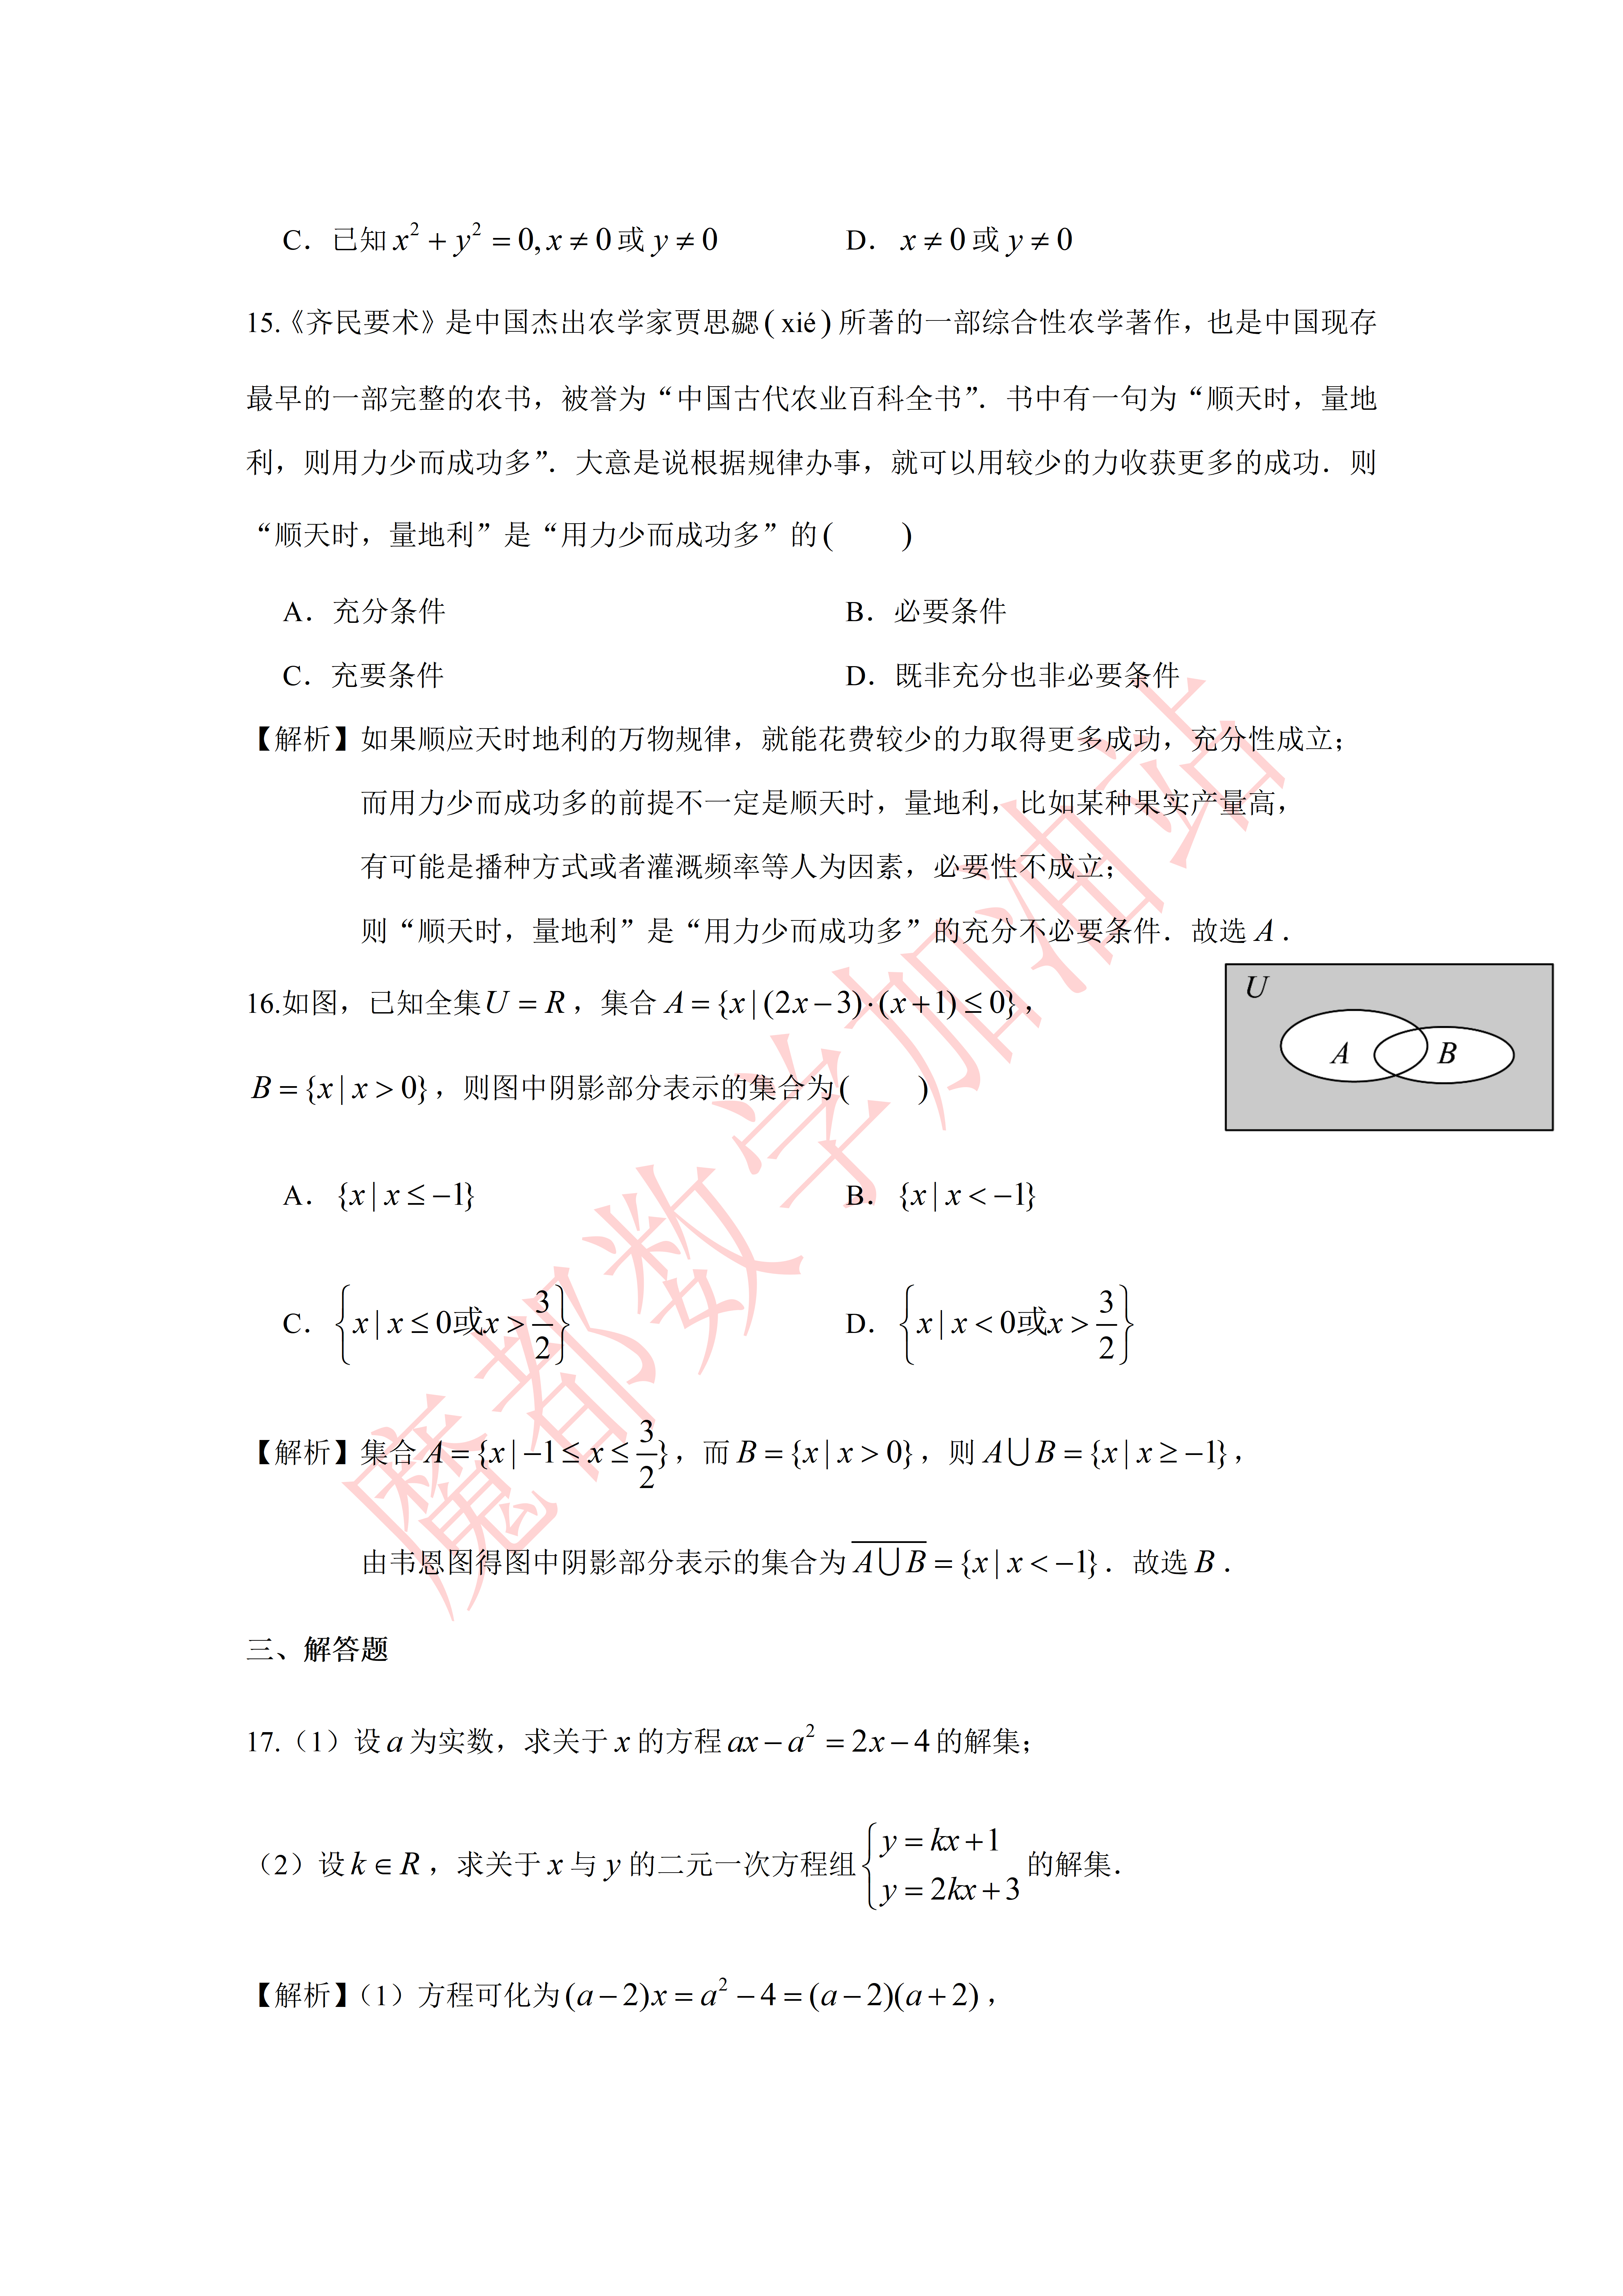
\includegraphics[width=.34\linewidth,trim=3586bp 3410bp 196bp 2818bp,clip]{../原图/高一52_回民中学_9月月考/04.png}
\end{center}

\keepwithprev
A. $\{x\mid x\leqslant-1\}$\qquad B. $\{x\mid x<-1\}$

C. $\left\{x\mid x\leqslant0\text{ 或 }x>\dfrac32\right\}$\qquad D. $\left\{x\mid x<0\text{ 或 }x>\dfrac32\right\}$

\ifanswer
\solbegin
\step{集合 $A=\left\{x\mid-1\leqslant x\leqslant\dfrac32\right\}$，而 $B=\{x\mid x>0\}$，则 $A\cup B=\{x\mid x\geqslant-1\}$，}
\step{由韦恩图得图中阴影部分表示的集合为 $\overline{A\cup B}=\{x\mid x<-1\}$．故选 $B$．}
\solend
\fi

\end{enumerate}

\bigsec{三、解答题}

\begin{enumerate}
\setcounter{enumi}{16}

\item （1）设 $a$ 为实数，求关于 $x$ 的方程 $ax-a^2=2x-4$ 的解集；

（2）设 $k\in\R$，求关于 $x$ 与 $y$ 的二元一次方程组 $\begin{cases}y=kx+1\\y=2kx+3\end{cases}$ 的解集．

\ifanswer
\solbegin
\stepm{(1)}{方程可化为 $(a-2)x=a^2-4=(a-2)(a+2)$，}
\step{当 $a\neq2$ 时，方程的解为 $x=\dfrac{(a-2)(a+2)}{a-2}=a+2$，则解集为 $\{a+2\}$；}
\step{当 $a=2$ 时，方程为 $2x-4=2x-4$，对 $x$ 取一切实数均成立，}
\step{所以解集为 $\R$；}
\stepm{(2)}{$\begin{cases}y=kx+1\\y=2kx+3\end{cases}$，则 $kx+1=2kx+3,kx=-2$，}
\step{当 $k=0$ 时，等式不成立，无解；当 $k\neq0$ 时，$x=-\dfrac2k,y=-1$；}
\step{综上所述，当 $k=0$ 时，解集为 $\varnothing$；当 $k\neq0$ 时，解集为 $\left\{\left(-\dfrac2k,-1\right)\right\}$．}
\solend
\fi

\ansspace[6]

\item 已知命题 $p$：方程 $x^2+6x+m-1=0$ 有两个不等的负根；命题 $q$：方程 $9x^2+6x+m-2=0$ 无实根．

\begin{enumerate}[label=(\arabic*)]
\item 若 $p$ 为真命题，求实数 $m$ 的取值范围；
\item 若 $p,q$ 两命题一真一假，求实数 $m$ 的取值范围．
\end{enumerate}

\ifanswer
\solbegin
\stepm{(1)}{设方程 $x^2+6x+m-1=0$ 两根为 $x_1,x_2$，}
\step{则 $\begin{cases}\Delta>0\\ x_1+x_2<0\\ x_1x_2>0\end{cases}\Rightarrow\begin{cases}36-4(m-1)>0\\ -6<0\\ m-1>0\end{cases}\Rightarrow1<m<10$；}
\stepm{(2)}{若命题 $q$ 为真命题，则 $36-36(m-2)<0\Rightarrow m>3$，}
\step{从而当命题 $q$ 为假命题时，$m\leqslant3$；}
\step{又由（1）得 $p$ 为假命题时，$m\leqslant1$ 或 $m\geqslant10$；}
\step{则当 $p$ 为真命题，$q$ 为假命题时，得 $\begin{cases}1<m<10\\ m\leqslant3\end{cases}\Rightarrow1<m\leqslant3$；}
\step{当 $q$ 为真命题，$p$ 为假命题时，得 $\begin{cases}m\leqslant1\text{ 或 }m\geqslant10\\ m>3\end{cases}\Rightarrow m\geqslant10$；}
\step{综上，当 $p,q$ 两命题一真一假时，$1<m\leqslant3$ 或 $m\geqslant10$.}
\solend
\fi

\ansspace[6]

\item 证明下列两个命题：

\begin{enumerate}[label=(\arabic*)]
\item 设 $ab>0$，求证：$a>b$ 是 $\dfrac1a<\dfrac1b$ 的充要条件．
\item 已知 $a,b$ 为正数，$n$ 为正整数，求证：如果 $a^n>b^n$，那么 $a>b$．
\end{enumerate}

\ifanswer
\solbegin
\stepm{(1)}{先证充分性：因为 $ab>0$ 且 $a>b$，故 $a-b>0$，从而 $\dfrac{a-b}{ab}>0$，}
\step{即 $\dfrac1b-\dfrac1a>0$，即 $\dfrac1a<\dfrac1b$；}
\step{再证必要性：若 $\dfrac1a<\dfrac1b$，则 $\dfrac1a-\dfrac1b=\dfrac{b-a}{ab}<0$，}
\step{又因为 $ab>0$，所以 $b-a<0$，即 $a>b$．}
% 原卷如此，照录未改（第 19 题(1)此句末用全角句号“。”，全卷其余各题末句用“．”，
% 见文件头“原卷笔误/存疑”第 4 条）
\step{综上，$a>b$ 是 $\dfrac1a<\dfrac1b$ 的充要条件。}
\stepm{(2)}{令 $f(x)=x^n,n\in\N^*$，则由幂函数的性质得 $f(x)$ 在第一象限是严格增的，}
\step{而 $a^n>b^n$ 即意味着 $f(a)>f(b)$，且 $a,b$ 为正数，从而 $a>b$．}
\solend
\fi

\ansspace[8]

\item （1）求关于 $x$ 的不等式 $(m-2)x>1-m$ 的解集；

（2）求关于 $x$ 的不等式 $x^2-(a+1)x+a\leqslant0$ 的解集．

\ifanswer
\solbegin
\stepm{(1)}{由不等式 $(m-2)x>1-m$，}
\step{当 $m-2>0$ 时，即 $m>2$ 时，解得 $x>\dfrac{1-m}{m-2}$，}
\step{所以不等式的解集为 $\left(\dfrac{1-m}{m-2},+\infty\right)$；}
\step{当 $m-2=0$ 时，即 $m=2$ 时，不等式即为 $0>-1$ 恒成立，}
\step{即不等式的解集为 $\R$；}
\step{当 $m-2<0$ 时，即 $m<2$ 时，解得 $x<\dfrac{1-m}{m-2}$，}
\step{所以不等式的解集为 $\left(-\infty,\dfrac{1-m}{m-2}\right)$；}
\step{综上，当 $m>2$ 时，解集为 $\left(\dfrac{1-m}{m-2},+\infty\right)$；}
\step{当 $m=2$ 时，解集为 $\R$；}
\step{当 $m<2$ 时，解集为 $\left(-\infty,\dfrac{1-m}{m-2}\right)$．}
\stepm{(2)}{由不等式 $x^2-(a+1)x+a\leqslant0$，可化为 $(x-a)(x-1)\leqslant0$，}
\step{当 $a>1$ 时，解得 $1\leqslant x\leqslant a$，即不等式的解集为 $[1,a]$；}
\step{当 $a=1$ 时，不等式即为 $(x-1)^2\leqslant0$，解得 $x=1$，即不等式的解集为 $\{1\}$；}
\step{当 $a<1$ 时，解得 $a\leqslant x\leqslant1$，即不等式的解集为 $[a,1]$，}
\step{综上，当 $a>1$ 时，解集为 $[1,a]$；}
\step{当 $a=1$ 时，解集为 $\{1\}$；}
\step{当 $a<1$ 时，解集为 $[a,1]$．}
\solend
\fi

\ansspace[10]

\item 已知集合 $A=\{x\mid(x+2)(5-x)\geqslant0\}$，若集合 $B$ 满足 $A\cap B=\varnothing,A\cup B=[-2,7)$．

\begin{enumerate}[label=(\arabic*)]
\item 用区间表示集合 $B$；
\item 若集合 $B$ 是不等式 $-x^2+bx+c>0$ 的解集，求实数 $b,c$ 的值；
\item 已知全集为 $\R$，若关于 $x$ 的不等式 $-1<x-a\leqslant2$ 的解集为 $M$，且“$x\in\overline A$”是“$x\in M$”的必要非充分条件，求实数 $a$ 的取值范围．
\end{enumerate}

\ifanswer
\solbegin
\stepm{(1)}{由题意得 $(x+2)(5-x)\geqslant0\Leftrightarrow(x+2)(x-5)\leqslant0\Rightarrow-2\leqslant x\leqslant5$，}
\step{则 $A=[-2,5]$，又 $A\cap B=\varnothing,A\cup B=[-2,7)$，则 $B=(5,7)$；}
\stepm{(2)}{$-x^2+bx+c>0\Leftrightarrow x^2-bx-c<0$，则 $x^2-bx-c=0$ 两根为 $5,7$，}
\step{则由韦达定理得 $b=12,-c=35\Rightarrow c=-35$；}
\stepm{(3)}{由题意得 $M=(a-1,a+2],\overline A=(-\infty,-2)\cup(5,+\infty)$，}
\step{且“$x\in\overline A$”是“$x\in M$”的必要非充分条件，则 $M$ 是 $\overline A$ 的真子集，}
\step{从而 $a+2<-2$ 或 $a-1\geqslant5$，解得 $a<-4$ 或 $a\geqslant6$，}
\step{所以实数 $a$ 的取值范围为 $(-\infty,-4)\cup[6,+\infty)$．}
\solend
\fi

\ansspace*[10]

\end{enumerate}

\end{document}
"
%
% 原始材料：微信公众号“魔都数学加油站”文章，作者破晓，连载“27学年高一52”；
% 原文标题“27学年高一52——2026-2027年上海市回民中学高一上9月月考”；
% 原文链接：https://mp.weixin.qq.com/s/ndjyozrRQCLl4ba3J8uR7g。
% 该页面用 JS 渲染，未见明确发布日期；页面内时间戳约为 2026-10-06 21:19／21:38，本稿以该时刻记可得日期。
% 正文为 8 张 PNG 页：第 01—07 页 4762×6735，第 08 页 2560×3620（**同一篇各页分辨率不同**），
% 均按页序读取。8 页全为试卷正文页（卷首标题在第 1 页页顶，卷末解答题第 21 题解析止于第 8 页），
% 无封面页、目录页、二维码或宣传页。粉色斜排“魔都数学加油站”为卷面水印，与公众号页脚一并未录入。
%
% 卷首标题：照卷面印作“2026--2027 年回民中学高一上 9 月月考”（公众号标题中的“上海市”
% 卷面标题行没有，本稿照卷面），年份区间按全稿惯例排 en dash。原卷只有一行标题、无副标题。
%
% 篇幅与题号：原卷自第 3 题起编号（第 1、2 题不在本卷内）。填空题 3—12（10 题）、
% 选择题 13—16（4 题）、解答题 17—21（5 题），共 19 题。本稿沿用原节与原题号，
% 只改排为全稿统一的大节样式（原卷小节标题为“一、填空题”“二、选择题”“三、解答题”）。
%
% 讲评版：原卷每题下直接印【答案】或【解析】。**只印【答案】的 1 题**（第 3 题），本稿只给 \ans{}；
% **第 14 题没有任何【答案】/【解析】段**，答案“D”直接印在题干括号内（“应假设(  D  )”），
% 本稿按 高一37 第 13 题的成例把括号留空、答案另提为 \ans{$D$}；
% 其余 17 题都只印【解析】，按全稿口径这类题不另提 \ans{}——其中选择题第 13、15、16 题的结论
% 写在解析末句（“故选 A／A／B”），亦照录在解析内。
%
% 副标题：原卷未印副标题。本稿按“知识模块”口径标作“集合与常用逻辑用语、不等式”：
% 19 题中集合与常用逻辑用语 10 题（集合类 7 题——第 3、4、5、9、12、16、21 题；
% 逻辑类 3 题——第 6、14、15 题），不等式 9 题（含等式性质与一元二次方程：第 7、8、10、11、
% 13、17、18、19、20 题），两类均远超三分之一，故并标。口径同 高一46、高一47、高一48、高一51。
%
% 与原卷的排版差异：
%   ① 原卷每题下直接印【答案】/【解析】，本稿按全稿惯例将答案与解析置于答案版，试卷版保持干净；
%      第 14 题印在题干括号内的答案“D”同样移入 \ans{}，见上；
%   ② 原卷未印副标题，本稿按“知识模块”口径补出；
%   ③ 原卷填空横线约两个字宽，本稿按全稿惯例统一排 \blankline[4.4em]；
%      选择题的作答括号原卷排半角“(    )”，本稿按全稿惯例排 \mbox{（\quad）}；
%   ④ 原卷实数集、自然数集排斜体/粗体 $R$、$\mathbf{R}$、$N$，本稿按全稿惯例改用 $\R$、$\N$；
%      空集记号统一为 \varnothing；
%   ⑤ 第 8 题题干与解析两处“两个实数分别为 $x_1$、$x_2$”原卷即用顿号，第 10、13 题等处
%      原卷在数学式内用半角逗号（如 $x_1,x_2$、$a,b,c\in R$），两份均照录未强改；
%      句末句点按全稿惯例排西文句点，句中句点（第 9、12、15、21 题）照原卷排全角“．”；
%   ⑥ 第 17、20 题原卷把子问标号“（1）”排在该题题号同一行，本稿照原卷仍排同一行（同 高一34 的
%      做法）；第 18、19、21 题的子问原卷各自另起一行，本稿按全稿惯例用 enumerate 的 (1)(2)(3)；
%      解析中的子问标号一律用 \stepm{(1)}{…}；
%   ⑦ 第 16 题的韦恩图原卷排在题干与选项右侧的浮动位置，本稿居中排在题干之后、选项之前，
%      并加 \needvspace 整块推走（守卫写在 \item 之前）；图自原图第 4 页裁切（trim），不另存图片文件；
%   ⑧ 每道解答题原卷未留作答空白，本稿按全稿惯例加 \ansspace。
%
% 原卷笔误/存疑（均照录未改，正文对应处另有 % 注）：
%   1. 第 8 题题干与解析首行两处均作“两个实数分别为 $x_1$、$x_2$”，按文意应为“两个实数**根**”
%      （疑脱“根”字，第 10 题同位置作“两个实根分别是”）；
%   2. 第 4 题解析“满足条件的 $A$ 的个数为集合 $\{0,1,3\}$ 的真子集，即 7 个”，
%      “个数为……真子集”表述不严（应为“……的真子集的个数”）；$\{0,1,3\}$ 的真子集 7 个，结论无误；
%   3. 第 6 题解析第 2 行“当 $a=10,b=0.2$ 时，$a+b>2$，且 $ab>1$，所以 $a>1$，且 $b>1$ 不成立”
%      ——此处是举反例，“所以”按文意应为“但”（$a=10,b=0.2$ 与“$a>1$ 且 $b>1$”不成立之间是转折，
%      非因果）；
%   4. 第 19 题 (1) 解析末行“综上，$a>b$ 是 $\dfrac1a<\dfrac1b$ 的充要条件。”用全角句号“。”，
%      全卷其余各题末句均用“．”，体例不一，照录；
%   5. 第 20 题第 (1) 问解析先按 $m>2$、$m=2$、$m<2$ 三种情况各给出解集，末三行又“综上”重述一遍，
%      与原卷一致（内容重复，非笔误）；
%   6. 第 18 题题干第 (2) 问“若 $p,q$ 两命题一真一假”，正文照录原卷所用半角逗号（未改顿号）。
%
% 插图：1 张，自原图裁切（无 \begin{tikzpicture} 重排）：
%   · 第 16 题题干韦恩图（全集 $U$ 矩形内两相交椭圆 $A$、$B$，灰色为阴影部分）
%     ——原图第 04 页，原卷排于题干与选项右侧。
%     裁框：x 3594–4558、y 2826–3317（即矩形外框，四周各留 4px），
%     trim=3590bp 3414bp 200bp 2822bp（左／下／右／上），页宽 4762、页高 6735。
%
\documentclass[a4paper,11pt]{article}
\usepackage{common}

\begin{document}

\examtitlest[3]{2026--2027 年回民中学高一上 9 月月考}{集合与常用逻辑用语、不等式}

\bigsec{一、填空题}

\begin{enumerate}
\setcounter{enumi}{2}

\item 用列举法写出下列集合 $\{(x,y)\mid x+y=2,x\in\N,y\in\N\}=$\blankline[4.4em].

\ifanswer
\ans{$\{(0,2),(1,1),(2,0)\}$}
\fi

\item 设集合 $A$ 满足 $\{-1,2\}\sub A\subset\{-1,0,1,2,3\}$，则满足条件的 $A$ 有\blankline[4.4em]个.

\ifanswer
\solbegin
\step{满足条件的 $A$ 的个数为集合 $\{0,1,3\}$ 的真子集，即 $7$ 个.}
\solend
\fi

\item 已知集合 $A=\{2,(a+1)^2,a^2+2\}$，且 $1\in A$，则实数 $a$ 的值为\blankline[4.4em].

\ifanswer
\solbegin
\step{因为 $1\in A$，而 $a^2+2\geqslant2$，所以 $(a+1)^2=1$，解得 $a=0$ 或 $a=-2$，}
\step{$a=0$ 时，$a^2+2=2$，不合题意，$a=-2$ 时，$a^2+2=6$，满足题意，}
\step{所以 $a=-2$.}
\solend
\fi

\item 已知 $a,b$ 是实数，则“$a>1$，且 $b>1$”是“$a+b>2$，且 $ab>1$”的\blankline[4.4em]条件.

\ifanswer
\solbegin
\step{$a,b$ 是实数，则“$a>1$，且 $b>1$”$\Rightarrow$“$a+b>2$，且 $ab>1$”正确，}
% 原卷如此，照录未改（第 6 题解析此处作“所以 $a>1$，且 $b>1$ 不成立”，按文意为转折，
% 见文件头“原卷笔误/存疑”第 3 条）
\step{当 $a=10,b=0.2$ 时，$a+b>2$，且 $ab>1$，所以 $a>1$，且 $b>1$ 不成立，}
\step{即前者是推出后者，后者推不出前者，}
\step{所以“$a>1$，且 $b>1$”是“$a+b>2$，且 $ab>1$”的充分而不必要条件.}
\solend
\fi

\item 已知等式 $2x^2-3x-1=a(x-1)^2+b(x-1)+c$ 恒成立，其中 $a,b,c$ 为常数，则 $a+b-c=$\blankline[4.4em].

\ifanswer
\solbegin
\step{将等式右侧展开整理得 $a(x-1)^2+b(x-1)+c=ax^2+(-2a+b)x+(a-b+c)$，}
\step{左右两边多项式恒等，对应次数的系数必须相等：}
\step{则 $a=2,-2a+b=-3$，代入 $a=2$ 得 $b=1$，$a-b+c=-1$，}
\step{代入 $a=2,b=1$ 得 $c=-2$，得 $a+b-c=2+1-(-2)=5$.}
\solend
\fi

% 原卷如此，照录未改（第 8 题题干与解析首行两处“两个实数分别为”疑脱“根”字，
% 见文件头“原卷笔误/存疑”第 1 条）
\item 若关于 $x$ 的二次方程 $x^2+mx+4m^2-3=0$ 的两个实数分别为 $x_1$、$x_2$，且满足 $x_1+x_2=x_1x_2$，则实数 $m$ 的值为\blankline[4.4em].

\ifanswer
\solbegin
% 原卷如此，照录未改（此处“两个实数分别为”同题干，疑脱“根”字）
\step{二次方程 $x^2+mx+4m^2-3=0$ 的两个实数分别为 $x_1$、$x_2$，}
\step{则有 $\Delta=m^2-4(4m^2-3)\geqslant0$，变形得 $m^2\leqslant\dfrac45$，}
\step{则 $x_1+x_2=-m$，$x_1x_2=(4m^2-3)$，}
\step{若 $x_1+x_2=x_1x_2$，则有 $-m=4m^2-3$，解得 $m=-1$ 或 $\dfrac34$，}
\step{又 $m^2\leqslant\dfrac45$，则 $m=\dfrac34$.}
\solend
\fi

\item 设集合 $A=\{x\mid x^2=1\}$，$B=\{x\mid ax=1\}$．若 $A\cap B=B$，则实数 $a$ 的值为\blankline[4.4em].

\ifanswer
\solbegin
\step{集合 $A=\{x\mid x^2=1\}=\{-1,1\}$，$B=\{x\mid ax=1\}$，$A\cap B=B$，所以 $B\sub A$，}
\step{当 $a=0$ 时，$B=\varnothing$，成立；}
\step{当 $a\neq0$ 时，$B=\left\{\dfrac1a\right\}$，则 $\dfrac1a=-1$ 或 $\dfrac1a=1$，解得 $a=-1$ 或 $a=1$，}
\step{所以实数 $a$ 的值为 $0$ 或 $1$ 或 $-1$.}
\solend
\fi

\item 已知关于 $x$ 的一元二次方程 $x^2+3x-3=0$ 的两个实根分别是 $x_1,x_2$，则以 $-\dfrac1{x_1},-\dfrac1{x_2}$ 为根且二次项系数是 $1$ 的一元二次方程为\blankline[4.4em].

\ifanswer
\solbegin
\step{因为 $x_1,x_2$ 是一元二次方程 $x^2+3x-3=0$ 的两个实根，}
\step{所以 $x_1+x_2=-3,x_1x_2=-3$，}
\step{所以 $-\dfrac1{x_1}+\left(-\dfrac1{x_2}\right)=-\dfrac{x_1+x_2}{x_1x_2}=-1$，$-\dfrac1{x_1}\cdot\left(-\dfrac1{x_2}\right)=\dfrac1{x_1x_2}=-\dfrac13$，}
\step{所以一元二次方程为 $x^2+x-\dfrac13=0$.}
\solend
\fi

\item 若关于 $x$ 的不等式 $(a-2)x^2+2(a-2)x-4<0$ 的解集是 $\R$，则实数 $a$ 的取值范围是\blankline[4.4em].

\ifanswer
\solbegin
\step{当 $a=2$ 时，不等式化为 $-4<0$ 对于任意实数 $x$ 都成立，因此 $a=2$ 满足题意；}
\step{当 $a\neq2$ 时，要使关于 $x$ 的不等式 $(a-2)x^2+2(a-2)x-4<0$ 的解集为 $\R$，}
\step{则 $\begin{cases}a-2<0\\ \Delta=4(a-2)^2+16(a-2)<0\end{cases}$，解得 $-2<a<2$．}
\step{综上，$a$ 的取值范围为 $(-2,2]$．}
\solend
\fi

\item 设非空集合 $A$、$B$，定义 $A\times B=\{x\mid x\in(A\cup B),x\notin(A\cap B)\}$．已知 $A=\{x\mid0\leqslant x\leqslant2\}$，$B=\{y\mid y\geqslant0\}$，则 $A\times B=$\blankline[4.4em].

\ifanswer
\solbegin
\step{由于 $A=\{x\mid0\leqslant x\leqslant2\}$，$B=\{y\mid y\geqslant0\}=\{x\mid x\geqslant0\}$，}
\step{所以 $A\cup B=\{x\mid x\geqslant0\}$，$A\cap B=\{x\mid0\leqslant x\leqslant2\}$，故 $A\times B=\{x\mid x>2\}$．}
\solend
\fi

\end{enumerate}

\bigsec{二、选择题}

\begin{enumerate}
\setcounter{enumi}{12}

\item 已知 $a,b,c\in\R$ 且 $a>b$，则下列不等式一定成立的是\mbox{（\quad）}

\keepwithprev
A. $\dfrac{a}{c^2+1}>\dfrac{b}{c^2+1}$\qquad B. $\dfrac1a<\dfrac1b$

C. $ac>bc$\qquad D. $a^2>b^2$

\ifanswer
\solbegin
\step{对于 A：因为 $c^2+1>0$ 恒成立，且 $a>b$，所以 $\dfrac{a}{c^2+1}>\dfrac{b}{c^2+1}$ 一定成立，}
\step{所以 A 正确；}
\step{对于 B：当 $a=1,b=-1$ 时，满足 $a>b$，此时 $\dfrac1a=1>\dfrac1b=-1$，所以 B 错误；}
\step{对于 C：当 $c<0$ 时，由 $a>b$，得 $ac<bc$，所以 C 错误；}
\step{对于 D：当 $a=1,b=-2$ 时，满足 $a>b$，此时 $a^2=1<b^2=4$，所以 D 错误；}
\step{故选 $A$．}
\solend
\fi

% 注：本题的答案“D”原卷直接印在题干末尾的括号内（“应假设(  D  )”），且没有单独的
%     【答案】/【解析】段，本稿按 高一37 第 13 题的成例把括号留空、另提为 \ans{}，
%     见文件头“与原卷的排版差异”①。
\item 用反证法证明：“已知 $x,y\in\R$,$x^2+y^2=0$，求证：$x=y=0$”时，应假设\mbox{（\quad）}

\keepwithprev
A. 已知 $x^2+y^2=0,x\neq0$ 且 $y\neq0$\qquad B. $x\neq0$ 且 $y\neq0$

C. 已知 $x^2+y^2=0,x\neq0$ 或 $y\neq0$\qquad D. $x\neq0$ 或 $y\neq0$

\ans{$D$}

\item 《齐民要术》是中国杰出农学家贾思勰（xié）所著的一部综合性农学著作，也是中国现存最早的一部完整的农书，被誉为“中国古代农业百科全书”．书中有一句为“顺天时，量地利，则用力少而成功多”．大意是说根据规律办事，就可以用较少的力收获更多的成功．则“顺天时，量地利”是“用力少而成功多”的\mbox{（\quad）}

\keepwithprev
A. 充分条件\qquad B. 必要条件

C. 充要条件\qquad D. 既非充分也非必要条件

\ifanswer
\solbegin
\step{如果顺应天时地利的万物规律，就能花费较少的力取得更多成功，充分性成立；}
\step{而用力少而成功多的前提不一定是顺天时，量地利，比如某种果实产量高，}
\step{有可能是播种方式或者灌溉频率等人为因素，必要性不成立；}
\step{则“顺天时，量地利”是“用力少而成功多”的充分不必要条件．故选 $A$．}
\solend
\fi

\needvspace{13\baselineskip}

\item 如图，已知全集 $U=\R$，集合 $A=\{x\mid(2x-3)\cdot(x+1)\leqslant0\}$，$B=\{x\mid x>0\}$，则图中阴影部分表示的集合为\mbox{（\quad）}

\begin{center}
% 原图第 4 页题干韦恩图直接裁取（原卷排于题干与选项右侧）。
% 裁框取矩形外框 x 3590–4558、y 2822–3321，再向外各留 4px（即 x 3586–4562、y 2818–3325），
% trim=左 3586bp／下 3410bp／右 196bp／上 2818bp（页宽 4762、页高 6735）。
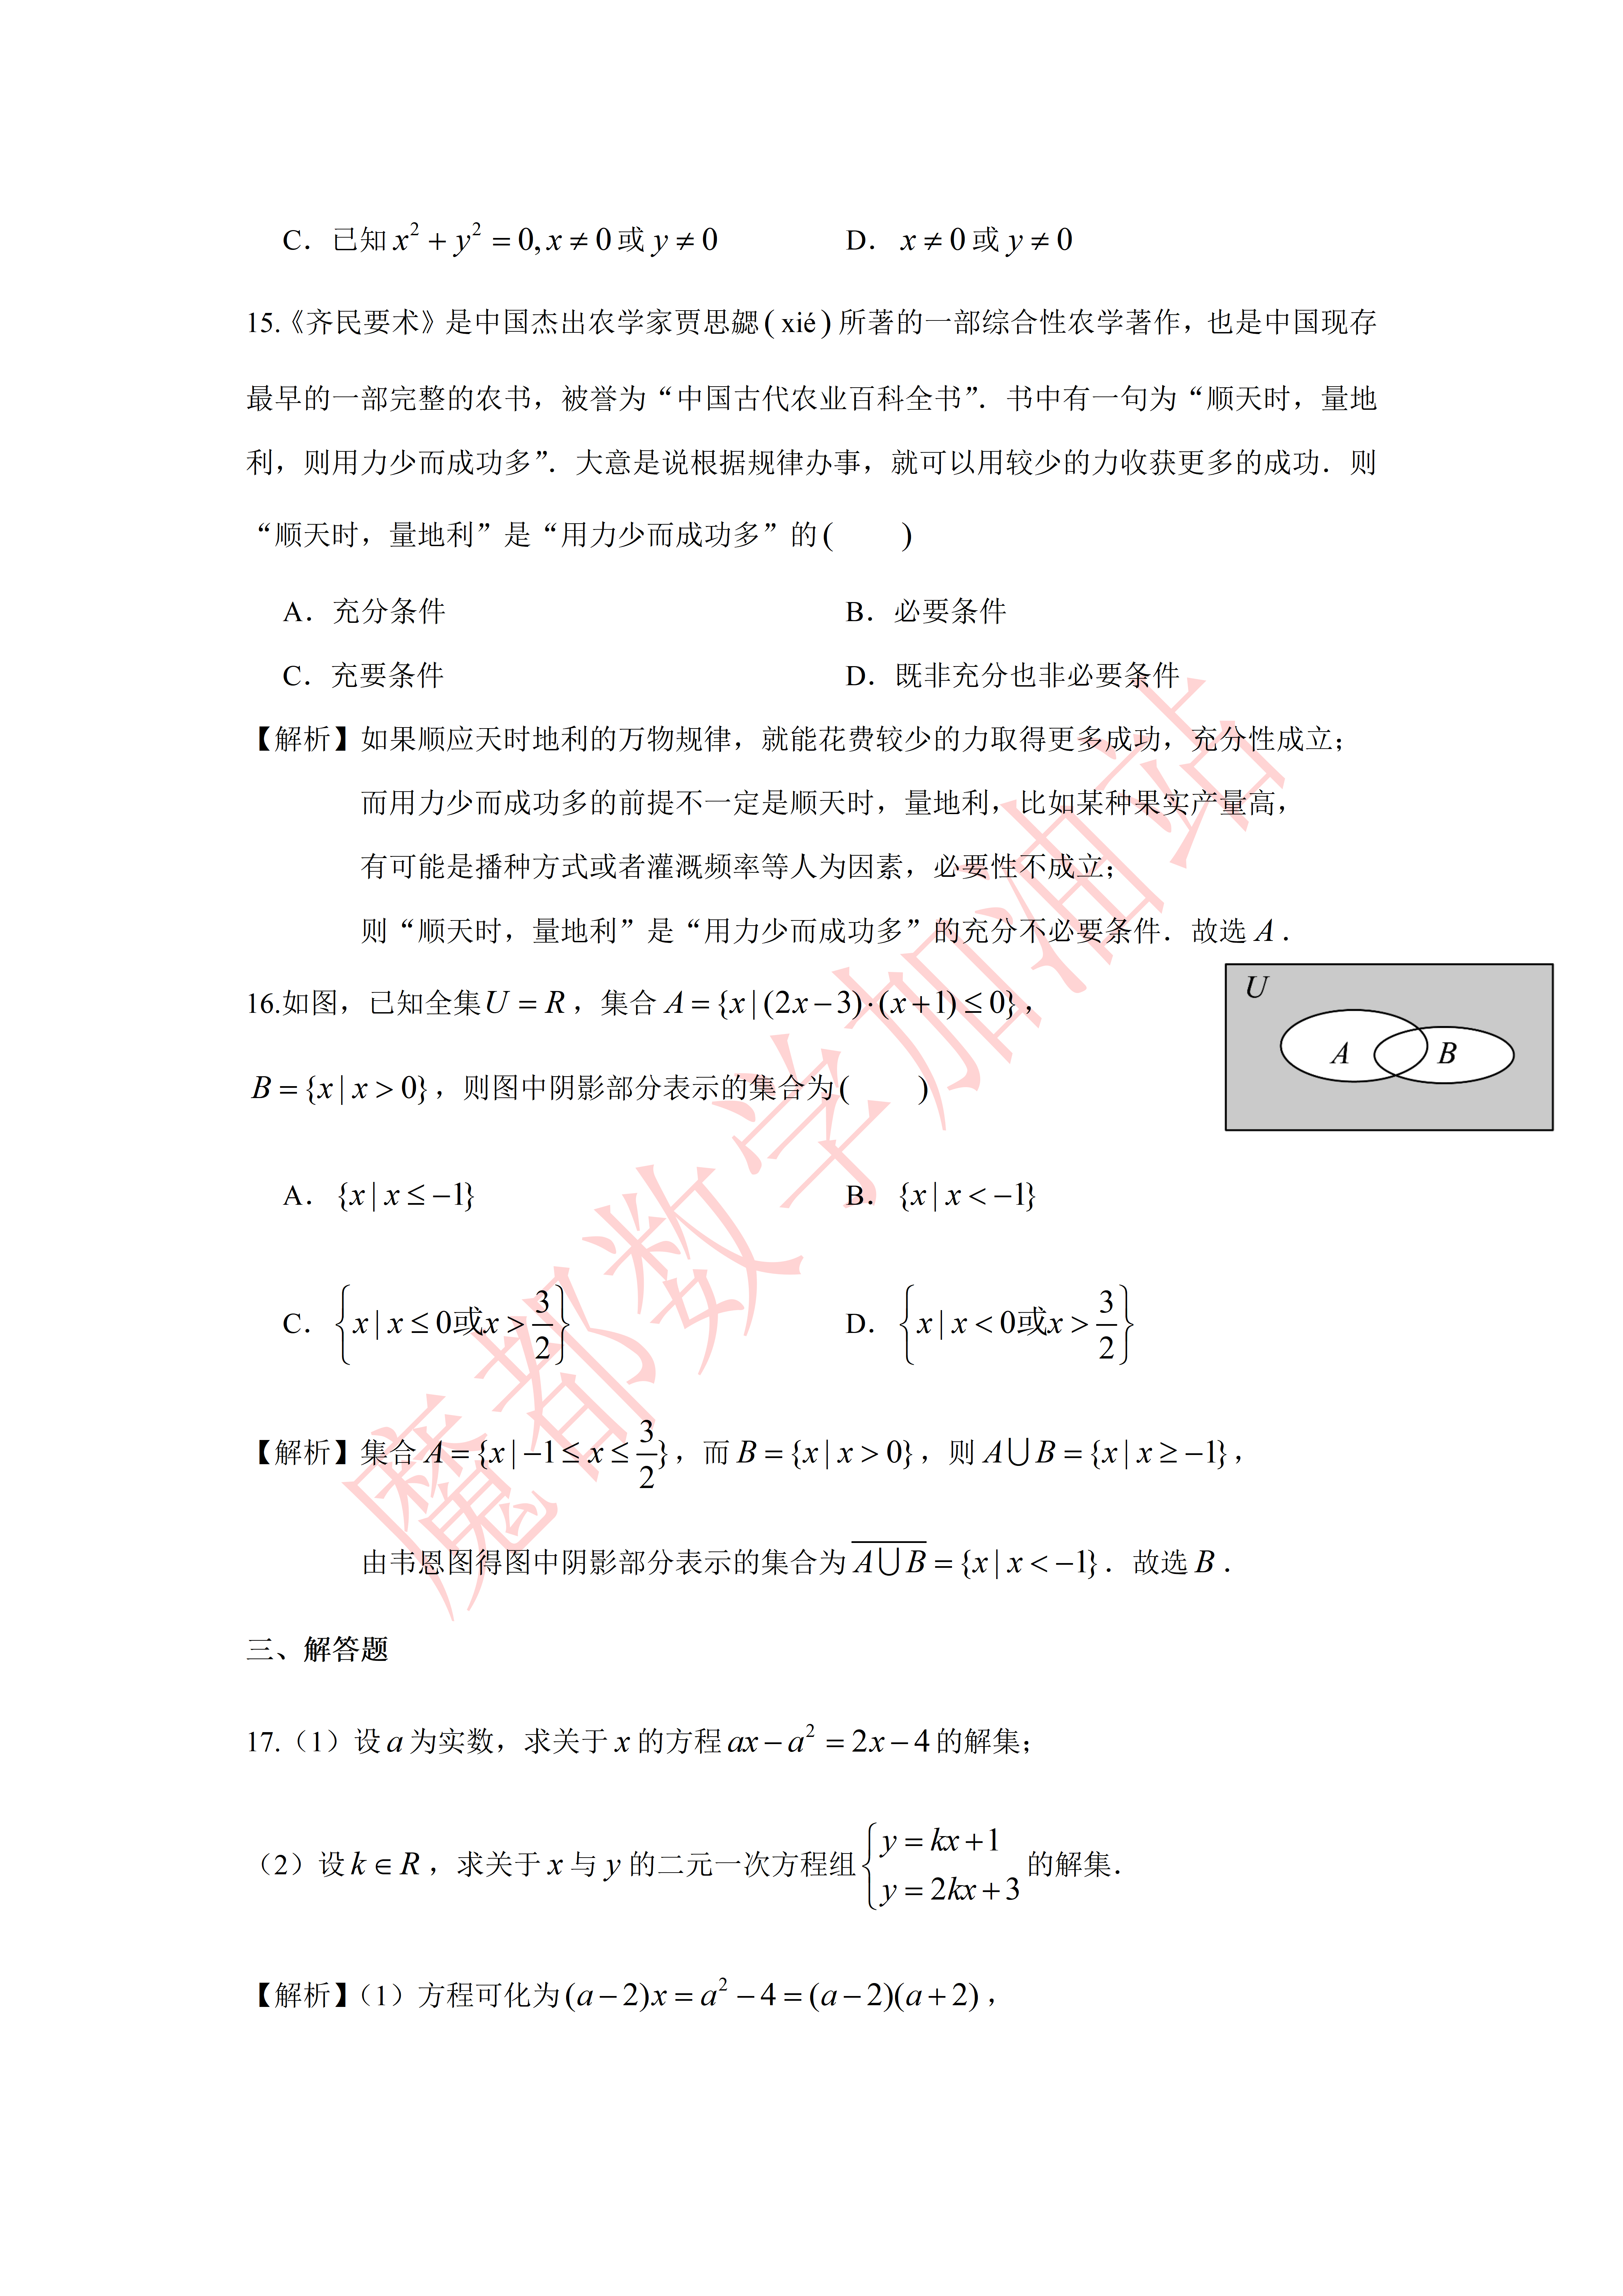
\includegraphics[width=.34\linewidth,trim=3586bp 3410bp 196bp 2818bp,clip]{../原图/高一52_回民中学_9月月考/04.png}
\end{center}

\keepwithprev
A. $\{x\mid x\leqslant-1\}$\qquad B. $\{x\mid x<-1\}$

C. $\left\{x\mid x\leqslant0\text{ 或 }x>\dfrac32\right\}$\qquad D. $\left\{x\mid x<0\text{ 或 }x>\dfrac32\right\}$

\ifanswer
\solbegin
\step{集合 $A=\left\{x\mid-1\leqslant x\leqslant\dfrac32\right\}$，而 $B=\{x\mid x>0\}$，则 $A\cup B=\{x\mid x\geqslant-1\}$，}
\step{由韦恩图得图中阴影部分表示的集合为 $\overline{A\cup B}=\{x\mid x<-1\}$．故选 $B$．}
\solend
\fi

\end{enumerate}

\bigsec{三、解答题}

\begin{enumerate}
\setcounter{enumi}{16}

\item （1）设 $a$ 为实数，求关于 $x$ 的方程 $ax-a^2=2x-4$ 的解集；

（2）设 $k\in\R$，求关于 $x$ 与 $y$ 的二元一次方程组 $\begin{cases}y=kx+1\\y=2kx+3\end{cases}$ 的解集．

\ifanswer
\solbegin
\stepm{(1)}{方程可化为 $(a-2)x=a^2-4=(a-2)(a+2)$，}
\step{当 $a\neq2$ 时，方程的解为 $x=\dfrac{(a-2)(a+2)}{a-2}=a+2$，则解集为 $\{a+2\}$；}
\step{当 $a=2$ 时，方程为 $2x-4=2x-4$，对 $x$ 取一切实数均成立，}
\step{所以解集为 $\R$；}
\stepm{(2)}{$\begin{cases}y=kx+1\\y=2kx+3\end{cases}$，则 $kx+1=2kx+3,kx=-2$，}
\step{当 $k=0$ 时，等式不成立，无解；当 $k\neq0$ 时，$x=-\dfrac2k,y=-1$；}
\step{综上所述，当 $k=0$ 时，解集为 $\varnothing$；当 $k\neq0$ 时，解集为 $\left\{\left(-\dfrac2k,-1\right)\right\}$．}
\solend
\fi

\ansspace[6]

\item 已知命题 $p$：方程 $x^2+6x+m-1=0$ 有两个不等的负根；命题 $q$：方程 $9x^2+6x+m-2=0$ 无实根．

\begin{enumerate}[label=(\arabic*)]
\item 若 $p$ 为真命题，求实数 $m$ 的取值范围；
\item 若 $p,q$ 两命题一真一假，求实数 $m$ 的取值范围．
\end{enumerate}

\ifanswer
\solbegin
\stepm{(1)}{设方程 $x^2+6x+m-1=0$ 两根为 $x_1,x_2$，}
\step{则 $\begin{cases}\Delta>0\\ x_1+x_2<0\\ x_1x_2>0\end{cases}\Rightarrow\begin{cases}36-4(m-1)>0\\ -6<0\\ m-1>0\end{cases}\Rightarrow1<m<10$；}
\stepm{(2)}{若命题 $q$ 为真命题，则 $36-36(m-2)<0\Rightarrow m>3$，}
\step{从而当命题 $q$ 为假命题时，$m\leqslant3$；}
\step{又由（1）得 $p$ 为假命题时，$m\leqslant1$ 或 $m\geqslant10$；}
\step{则当 $p$ 为真命题，$q$ 为假命题时，得 $\begin{cases}1<m<10\\ m\leqslant3\end{cases}\Rightarrow1<m\leqslant3$；}
\step{当 $q$ 为真命题，$p$ 为假命题时，得 $\begin{cases}m\leqslant1\text{ 或 }m\geqslant10\\ m>3\end{cases}\Rightarrow m\geqslant10$；}
\step{综上，当 $p,q$ 两命题一真一假时，$1<m\leqslant3$ 或 $m\geqslant10$.}
\solend
\fi

\ansspace[6]

\item 证明下列两个命题：

\begin{enumerate}[label=(\arabic*)]
\item 设 $ab>0$，求证：$a>b$ 是 $\dfrac1a<\dfrac1b$ 的充要条件．
\item 已知 $a,b$ 为正数，$n$ 为正整数，求证：如果 $a^n>b^n$，那么 $a>b$．
\end{enumerate}

\ifanswer
\solbegin
\stepm{(1)}{先证充分性：因为 $ab>0$ 且 $a>b$，故 $a-b>0$，从而 $\dfrac{a-b}{ab}>0$，}
\step{即 $\dfrac1b-\dfrac1a>0$，即 $\dfrac1a<\dfrac1b$；}
\step{再证必要性：若 $\dfrac1a<\dfrac1b$，则 $\dfrac1a-\dfrac1b=\dfrac{b-a}{ab}<0$，}
\step{又因为 $ab>0$，所以 $b-a<0$，即 $a>b$．}
% 原卷如此，照录未改（第 19 题(1)此句末用全角句号“。”，全卷其余各题末句用“．”，
% 见文件头“原卷笔误/存疑”第 4 条）
\step{综上，$a>b$ 是 $\dfrac1a<\dfrac1b$ 的充要条件。}
\stepm{(2)}{令 $f(x)=x^n,n\in\N^*$，则由幂函数的性质得 $f(x)$ 在第一象限是严格增的，}
\step{而 $a^n>b^n$ 即意味着 $f(a)>f(b)$，且 $a,b$ 为正数，从而 $a>b$．}
\solend
\fi

\ansspace[8]

\item （1）求关于 $x$ 的不等式 $(m-2)x>1-m$ 的解集；

（2）求关于 $x$ 的不等式 $x^2-(a+1)x+a\leqslant0$ 的解集．

\ifanswer
\solbegin
\stepm{(1)}{由不等式 $(m-2)x>1-m$，}
\step{当 $m-2>0$ 时，即 $m>2$ 时，解得 $x>\dfrac{1-m}{m-2}$，}
\step{所以不等式的解集为 $\left(\dfrac{1-m}{m-2},+\infty\right)$；}
\step{当 $m-2=0$ 时，即 $m=2$ 时，不等式即为 $0>-1$ 恒成立，}
\step{即不等式的解集为 $\R$；}
\step{当 $m-2<0$ 时，即 $m<2$ 时，解得 $x<\dfrac{1-m}{m-2}$，}
\step{所以不等式的解集为 $\left(-\infty,\dfrac{1-m}{m-2}\right)$；}
\step{综上，当 $m>2$ 时，解集为 $\left(\dfrac{1-m}{m-2},+\infty\right)$；}
\step{当 $m=2$ 时，解集为 $\R$；}
\step{当 $m<2$ 时，解集为 $\left(-\infty,\dfrac{1-m}{m-2}\right)$．}
\stepm{(2)}{由不等式 $x^2-(a+1)x+a\leqslant0$，可化为 $(x-a)(x-1)\leqslant0$，}
\step{当 $a>1$ 时，解得 $1\leqslant x\leqslant a$，即不等式的解集为 $[1,a]$；}
\step{当 $a=1$ 时，不等式即为 $(x-1)^2\leqslant0$，解得 $x=1$，即不等式的解集为 $\{1\}$；}
\step{当 $a<1$ 时，解得 $a\leqslant x\leqslant1$，即不等式的解集为 $[a,1]$，}
\step{综上，当 $a>1$ 时，解集为 $[1,a]$；}
\step{当 $a=1$ 时，解集为 $\{1\}$；}
\step{当 $a<1$ 时，解集为 $[a,1]$．}
\solend
\fi

\ansspace[10]

\item 已知集合 $A=\{x\mid(x+2)(5-x)\geqslant0\}$，若集合 $B$ 满足 $A\cap B=\varnothing,A\cup B=[-2,7)$．

\begin{enumerate}[label=(\arabic*)]
\item 用区间表示集合 $B$；
\item 若集合 $B$ 是不等式 $-x^2+bx+c>0$ 的解集，求实数 $b,c$ 的值；
\item 已知全集为 $\R$，若关于 $x$ 的不等式 $-1<x-a\leqslant2$ 的解集为 $M$，且“$x\in\overline A$”是“$x\in M$”的必要非充分条件，求实数 $a$ 的取值范围．
\end{enumerate}

\ifanswer
\solbegin
\stepm{(1)}{由题意得 $(x+2)(5-x)\geqslant0\Leftrightarrow(x+2)(x-5)\leqslant0\Rightarrow-2\leqslant x\leqslant5$，}
\step{则 $A=[-2,5]$，又 $A\cap B=\varnothing,A\cup B=[-2,7)$，则 $B=(5,7)$；}
\stepm{(2)}{$-x^2+bx+c>0\Leftrightarrow x^2-bx-c<0$，则 $x^2-bx-c=0$ 两根为 $5,7$，}
\step{则由韦达定理得 $b=12,-c=35\Rightarrow c=-35$；}
\stepm{(3)}{由题意得 $M=(a-1,a+2],\overline A=(-\infty,-2)\cup(5,+\infty)$，}
\step{且“$x\in\overline A$”是“$x\in M$”的必要非充分条件，则 $M$ 是 $\overline A$ 的真子集，}
\step{从而 $a+2<-2$ 或 $a-1\geqslant5$，解得 $a<-4$ 或 $a\geqslant6$，}
\step{所以实数 $a$ 的取值范围为 $(-\infty,-4)\cup[6,+\infty)$．}
\solend
\fi

\ansspace*[10]

\end{enumerate}

\end{document}
"
% 紧凑版：xelatex "\def\iscompact{1}% 高一52_回民中学_9月月考.tex
%   —— 高一上数学“2026-2027 年回民中学高一上 9 月月考”（讲评版）
% 试卷版：xelatex 高一52_回民中学_9月月考.tex
% 答案版：xelatex "\def\isanswer{1}% 高一52_回民中学_9月月考.tex
%   —— 高一上数学“2026-2027 年回民中学高一上 9 月月考”（讲评版）
% 试卷版：xelatex 高一52_回民中学_9月月考.tex
% 答案版：xelatex "\def\isanswer{1}\input{高一52_回民中学_9月月考.tex}"
% 紧凑版：xelatex "\def\iscompact{1}\input{高一52_回民中学_9月月考.tex}"
%
% 原始材料：微信公众号“魔都数学加油站”文章，作者破晓，连载“27学年高一52”；
% 原文标题“27学年高一52——2026-2027年上海市回民中学高一上9月月考”；
% 原文链接：https://mp.weixin.qq.com/s/ndjyozrRQCLl4ba3J8uR7g。
% 该页面用 JS 渲染，未见明确发布日期；页面内时间戳约为 2026-10-06 21:19／21:38，本稿以该时刻记可得日期。
% 正文为 8 张 PNG 页：第 01—07 页 4762×6735，第 08 页 2560×3620（**同一篇各页分辨率不同**），
% 均按页序读取。8 页全为试卷正文页（卷首标题在第 1 页页顶，卷末解答题第 21 题解析止于第 8 页），
% 无封面页、目录页、二维码或宣传页。粉色斜排“魔都数学加油站”为卷面水印，与公众号页脚一并未录入。
%
% 卷首标题：照卷面印作“2026--2027 年回民中学高一上 9 月月考”（公众号标题中的“上海市”
% 卷面标题行没有，本稿照卷面），年份区间按全稿惯例排 en dash。原卷只有一行标题、无副标题。
%
% 篇幅与题号：原卷自第 3 题起编号（第 1、2 题不在本卷内）。填空题 3—12（10 题）、
% 选择题 13—16（4 题）、解答题 17—21（5 题），共 19 题。本稿沿用原节与原题号，
% 只改排为全稿统一的大节样式（原卷小节标题为“一、填空题”“二、选择题”“三、解答题”）。
%
% 讲评版：原卷每题下直接印【答案】或【解析】。**只印【答案】的 1 题**（第 3 题），本稿只给 \ans{}；
% **第 14 题没有任何【答案】/【解析】段**，答案“D”直接印在题干括号内（“应假设(  D  )”），
% 本稿按 高一37 第 13 题的成例把括号留空、答案另提为 \ans{$D$}；
% 其余 17 题都只印【解析】，按全稿口径这类题不另提 \ans{}——其中选择题第 13、15、16 题的结论
% 写在解析末句（“故选 A／A／B”），亦照录在解析内。
%
% 副标题：原卷未印副标题。本稿按“知识模块”口径标作“集合与常用逻辑用语、不等式”：
% 19 题中集合与常用逻辑用语 10 题（集合类 7 题——第 3、4、5、9、12、16、21 题；
% 逻辑类 3 题——第 6、14、15 题），不等式 9 题（含等式性质与一元二次方程：第 7、8、10、11、
% 13、17、18、19、20 题），两类均远超三分之一，故并标。口径同 高一46、高一47、高一48、高一51。
%
% 与原卷的排版差异：
%   ① 原卷每题下直接印【答案】/【解析】，本稿按全稿惯例将答案与解析置于答案版，试卷版保持干净；
%      第 14 题印在题干括号内的答案“D”同样移入 \ans{}，见上；
%   ② 原卷未印副标题，本稿按“知识模块”口径补出；
%   ③ 原卷填空横线约两个字宽，本稿按全稿惯例统一排 \blankline[4.4em]；
%      选择题的作答括号原卷排半角“(    )”，本稿按全稿惯例排 \mbox{（\quad）}；
%   ④ 原卷实数集、自然数集排斜体/粗体 $R$、$\mathbf{R}$、$N$，本稿按全稿惯例改用 $\R$、$\N$；
%      空集记号统一为 \varnothing；
%   ⑤ 第 8 题题干与解析两处“两个实数分别为 $x_1$、$x_2$”原卷即用顿号，第 10、13 题等处
%      原卷在数学式内用半角逗号（如 $x_1,x_2$、$a,b,c\in R$），两份均照录未强改；
%      句末句点按全稿惯例排西文句点，句中句点（第 9、12、15、21 题）照原卷排全角“．”；
%   ⑥ 第 17、20 题原卷把子问标号“（1）”排在该题题号同一行，本稿照原卷仍排同一行（同 高一34 的
%      做法）；第 18、19、21 题的子问原卷各自另起一行，本稿按全稿惯例用 enumerate 的 (1)(2)(3)；
%      解析中的子问标号一律用 \stepm{(1)}{…}；
%   ⑦ 第 16 题的韦恩图原卷排在题干与选项右侧的浮动位置，本稿居中排在题干之后、选项之前，
%      并加 \needvspace 整块推走（守卫写在 \item 之前）；图自原图第 4 页裁切（trim），不另存图片文件；
%   ⑧ 每道解答题原卷未留作答空白，本稿按全稿惯例加 \ansspace。
%
% 原卷笔误/存疑（均照录未改，正文对应处另有 % 注）：
%   1. 第 8 题题干与解析首行两处均作“两个实数分别为 $x_1$、$x_2$”，按文意应为“两个实数**根**”
%      （疑脱“根”字，第 10 题同位置作“两个实根分别是”）；
%   2. 第 4 题解析“满足条件的 $A$ 的个数为集合 $\{0,1,3\}$ 的真子集，即 7 个”，
%      “个数为……真子集”表述不严（应为“……的真子集的个数”）；$\{0,1,3\}$ 的真子集 7 个，结论无误；
%   3. 第 6 题解析第 2 行“当 $a=10,b=0.2$ 时，$a+b>2$，且 $ab>1$，所以 $a>1$，且 $b>1$ 不成立”
%      ——此处是举反例，“所以”按文意应为“但”（$a=10,b=0.2$ 与“$a>1$ 且 $b>1$”不成立之间是转折，
%      非因果）；
%   4. 第 19 题 (1) 解析末行“综上，$a>b$ 是 $\dfrac1a<\dfrac1b$ 的充要条件。”用全角句号“。”，
%      全卷其余各题末句均用“．”，体例不一，照录；
%   5. 第 20 题第 (1) 问解析先按 $m>2$、$m=2$、$m<2$ 三种情况各给出解集，末三行又“综上”重述一遍，
%      与原卷一致（内容重复，非笔误）；
%   6. 第 18 题题干第 (2) 问“若 $p,q$ 两命题一真一假”，正文照录原卷所用半角逗号（未改顿号）。
%
% 插图：1 张，自原图裁切（无 \begin{tikzpicture} 重排）：
%   · 第 16 题题干韦恩图（全集 $U$ 矩形内两相交椭圆 $A$、$B$，灰色为阴影部分）
%     ——原图第 04 页，原卷排于题干与选项右侧。
%     裁框：x 3594–4558、y 2826–3317（即矩形外框，四周各留 4px），
%     trim=3590bp 3414bp 200bp 2822bp（左／下／右／上），页宽 4762、页高 6735。
%
\documentclass[a4paper,11pt]{article}
\usepackage{common}

\begin{document}

\examtitlest[3]{2026--2027 年回民中学高一上 9 月月考}{集合与常用逻辑用语、不等式}

\bigsec{一、填空题}

\begin{enumerate}
\setcounter{enumi}{2}

\item 用列举法写出下列集合 $\{(x,y)\mid x+y=2,x\in\N,y\in\N\}=$\blankline[4.4em].

\ifanswer
\ans{$\{(0,2),(1,1),(2,0)\}$}
\fi

\item 设集合 $A$ 满足 $\{-1,2\}\sub A\subset\{-1,0,1,2,3\}$，则满足条件的 $A$ 有\blankline[4.4em]个.

\ifanswer
\solbegin
\step{满足条件的 $A$ 的个数为集合 $\{0,1,3\}$ 的真子集，即 $7$ 个.}
\solend
\fi

\item 已知集合 $A=\{2,(a+1)^2,a^2+2\}$，且 $1\in A$，则实数 $a$ 的值为\blankline[4.4em].

\ifanswer
\solbegin
\step{因为 $1\in A$，而 $a^2+2\geqslant2$，所以 $(a+1)^2=1$，解得 $a=0$ 或 $a=-2$，}
\step{$a=0$ 时，$a^2+2=2$，不合题意，$a=-2$ 时，$a^2+2=6$，满足题意，}
\step{所以 $a=-2$.}
\solend
\fi

\item 已知 $a,b$ 是实数，则“$a>1$，且 $b>1$”是“$a+b>2$，且 $ab>1$”的\blankline[4.4em]条件.

\ifanswer
\solbegin
\step{$a,b$ 是实数，则“$a>1$，且 $b>1$”$\Rightarrow$“$a+b>2$，且 $ab>1$”正确，}
% 原卷如此，照录未改（第 6 题解析此处作“所以 $a>1$，且 $b>1$ 不成立”，按文意为转折，
% 见文件头“原卷笔误/存疑”第 3 条）
\step{当 $a=10,b=0.2$ 时，$a+b>2$，且 $ab>1$，所以 $a>1$，且 $b>1$ 不成立，}
\step{即前者是推出后者，后者推不出前者，}
\step{所以“$a>1$，且 $b>1$”是“$a+b>2$，且 $ab>1$”的充分而不必要条件.}
\solend
\fi

\item 已知等式 $2x^2-3x-1=a(x-1)^2+b(x-1)+c$ 恒成立，其中 $a,b,c$ 为常数，则 $a+b-c=$\blankline[4.4em].

\ifanswer
\solbegin
\step{将等式右侧展开整理得 $a(x-1)^2+b(x-1)+c=ax^2+(-2a+b)x+(a-b+c)$，}
\step{左右两边多项式恒等，对应次数的系数必须相等：}
\step{则 $a=2,-2a+b=-3$，代入 $a=2$ 得 $b=1$，$a-b+c=-1$，}
\step{代入 $a=2,b=1$ 得 $c=-2$，得 $a+b-c=2+1-(-2)=5$.}
\solend
\fi

% 原卷如此，照录未改（第 8 题题干与解析首行两处“两个实数分别为”疑脱“根”字，
% 见文件头“原卷笔误/存疑”第 1 条）
\item 若关于 $x$ 的二次方程 $x^2+mx+4m^2-3=0$ 的两个实数分别为 $x_1$、$x_2$，且满足 $x_1+x_2=x_1x_2$，则实数 $m$ 的值为\blankline[4.4em].

\ifanswer
\solbegin
% 原卷如此，照录未改（此处“两个实数分别为”同题干，疑脱“根”字）
\step{二次方程 $x^2+mx+4m^2-3=0$ 的两个实数分别为 $x_1$、$x_2$，}
\step{则有 $\Delta=m^2-4(4m^2-3)\geqslant0$，变形得 $m^2\leqslant\dfrac45$，}
\step{则 $x_1+x_2=-m$，$x_1x_2=(4m^2-3)$，}
\step{若 $x_1+x_2=x_1x_2$，则有 $-m=4m^2-3$，解得 $m=-1$ 或 $\dfrac34$，}
\step{又 $m^2\leqslant\dfrac45$，则 $m=\dfrac34$.}
\solend
\fi

\item 设集合 $A=\{x\mid x^2=1\}$，$B=\{x\mid ax=1\}$．若 $A\cap B=B$，则实数 $a$ 的值为\blankline[4.4em].

\ifanswer
\solbegin
\step{集合 $A=\{x\mid x^2=1\}=\{-1,1\}$，$B=\{x\mid ax=1\}$，$A\cap B=B$，所以 $B\sub A$，}
\step{当 $a=0$ 时，$B=\varnothing$，成立；}
\step{当 $a\neq0$ 时，$B=\left\{\dfrac1a\right\}$，则 $\dfrac1a=-1$ 或 $\dfrac1a=1$，解得 $a=-1$ 或 $a=1$，}
\step{所以实数 $a$ 的值为 $0$ 或 $1$ 或 $-1$.}
\solend
\fi

\item 已知关于 $x$ 的一元二次方程 $x^2+3x-3=0$ 的两个实根分别是 $x_1,x_2$，则以 $-\dfrac1{x_1},-\dfrac1{x_2}$ 为根且二次项系数是 $1$ 的一元二次方程为\blankline[4.4em].

\ifanswer
\solbegin
\step{因为 $x_1,x_2$ 是一元二次方程 $x^2+3x-3=0$ 的两个实根，}
\step{所以 $x_1+x_2=-3,x_1x_2=-3$，}
\step{所以 $-\dfrac1{x_1}+\left(-\dfrac1{x_2}\right)=-\dfrac{x_1+x_2}{x_1x_2}=-1$，$-\dfrac1{x_1}\cdot\left(-\dfrac1{x_2}\right)=\dfrac1{x_1x_2}=-\dfrac13$，}
\step{所以一元二次方程为 $x^2+x-\dfrac13=0$.}
\solend
\fi

\item 若关于 $x$ 的不等式 $(a-2)x^2+2(a-2)x-4<0$ 的解集是 $\R$，则实数 $a$ 的取值范围是\blankline[4.4em].

\ifanswer
\solbegin
\step{当 $a=2$ 时，不等式化为 $-4<0$ 对于任意实数 $x$ 都成立，因此 $a=2$ 满足题意；}
\step{当 $a\neq2$ 时，要使关于 $x$ 的不等式 $(a-2)x^2+2(a-2)x-4<0$ 的解集为 $\R$，}
\step{则 $\begin{cases}a-2<0\\ \Delta=4(a-2)^2+16(a-2)<0\end{cases}$，解得 $-2<a<2$．}
\step{综上，$a$ 的取值范围为 $(-2,2]$．}
\solend
\fi

\item 设非空集合 $A$、$B$，定义 $A\times B=\{x\mid x\in(A\cup B),x\notin(A\cap B)\}$．已知 $A=\{x\mid0\leqslant x\leqslant2\}$，$B=\{y\mid y\geqslant0\}$，则 $A\times B=$\blankline[4.4em].

\ifanswer
\solbegin
\step{由于 $A=\{x\mid0\leqslant x\leqslant2\}$，$B=\{y\mid y\geqslant0\}=\{x\mid x\geqslant0\}$，}
\step{所以 $A\cup B=\{x\mid x\geqslant0\}$，$A\cap B=\{x\mid0\leqslant x\leqslant2\}$，故 $A\times B=\{x\mid x>2\}$．}
\solend
\fi

\end{enumerate}

\bigsec{二、选择题}

\begin{enumerate}
\setcounter{enumi}{12}

\item 已知 $a,b,c\in\R$ 且 $a>b$，则下列不等式一定成立的是\mbox{（\quad）}

\keepwithprev
A. $\dfrac{a}{c^2+1}>\dfrac{b}{c^2+1}$\qquad B. $\dfrac1a<\dfrac1b$

C. $ac>bc$\qquad D. $a^2>b^2$

\ifanswer
\solbegin
\step{对于 A：因为 $c^2+1>0$ 恒成立，且 $a>b$，所以 $\dfrac{a}{c^2+1}>\dfrac{b}{c^2+1}$ 一定成立，}
\step{所以 A 正确；}
\step{对于 B：当 $a=1,b=-1$ 时，满足 $a>b$，此时 $\dfrac1a=1>\dfrac1b=-1$，所以 B 错误；}
\step{对于 C：当 $c<0$ 时，由 $a>b$，得 $ac<bc$，所以 C 错误；}
\step{对于 D：当 $a=1,b=-2$ 时，满足 $a>b$，此时 $a^2=1<b^2=4$，所以 D 错误；}
\step{故选 $A$．}
\solend
\fi

% 注：本题的答案“D”原卷直接印在题干末尾的括号内（“应假设(  D  )”），且没有单独的
%     【答案】/【解析】段，本稿按 高一37 第 13 题的成例把括号留空、另提为 \ans{}，
%     见文件头“与原卷的排版差异”①。
\item 用反证法证明：“已知 $x,y\in\R$,$x^2+y^2=0$，求证：$x=y=0$”时，应假设\mbox{（\quad）}

\keepwithprev
A. 已知 $x^2+y^2=0,x\neq0$ 且 $y\neq0$\qquad B. $x\neq0$ 且 $y\neq0$

C. 已知 $x^2+y^2=0,x\neq0$ 或 $y\neq0$\qquad D. $x\neq0$ 或 $y\neq0$

\ans{$D$}

\item 《齐民要术》是中国杰出农学家贾思勰（xié）所著的一部综合性农学著作，也是中国现存最早的一部完整的农书，被誉为“中国古代农业百科全书”．书中有一句为“顺天时，量地利，则用力少而成功多”．大意是说根据规律办事，就可以用较少的力收获更多的成功．则“顺天时，量地利”是“用力少而成功多”的\mbox{（\quad）}

\keepwithprev
A. 充分条件\qquad B. 必要条件

C. 充要条件\qquad D. 既非充分也非必要条件

\ifanswer
\solbegin
\step{如果顺应天时地利的万物规律，就能花费较少的力取得更多成功，充分性成立；}
\step{而用力少而成功多的前提不一定是顺天时，量地利，比如某种果实产量高，}
\step{有可能是播种方式或者灌溉频率等人为因素，必要性不成立；}
\step{则“顺天时，量地利”是“用力少而成功多”的充分不必要条件．故选 $A$．}
\solend
\fi

\needvspace{13\baselineskip}

\item 如图，已知全集 $U=\R$，集合 $A=\{x\mid(2x-3)\cdot(x+1)\leqslant0\}$，$B=\{x\mid x>0\}$，则图中阴影部分表示的集合为\mbox{（\quad）}

\begin{center}
% 原图第 4 页题干韦恩图直接裁取（原卷排于题干与选项右侧）。
% 裁框取矩形外框 x 3590–4558、y 2822–3321，再向外各留 4px（即 x 3586–4562、y 2818–3325），
% trim=左 3586bp／下 3410bp／右 196bp／上 2818bp（页宽 4762、页高 6735）。
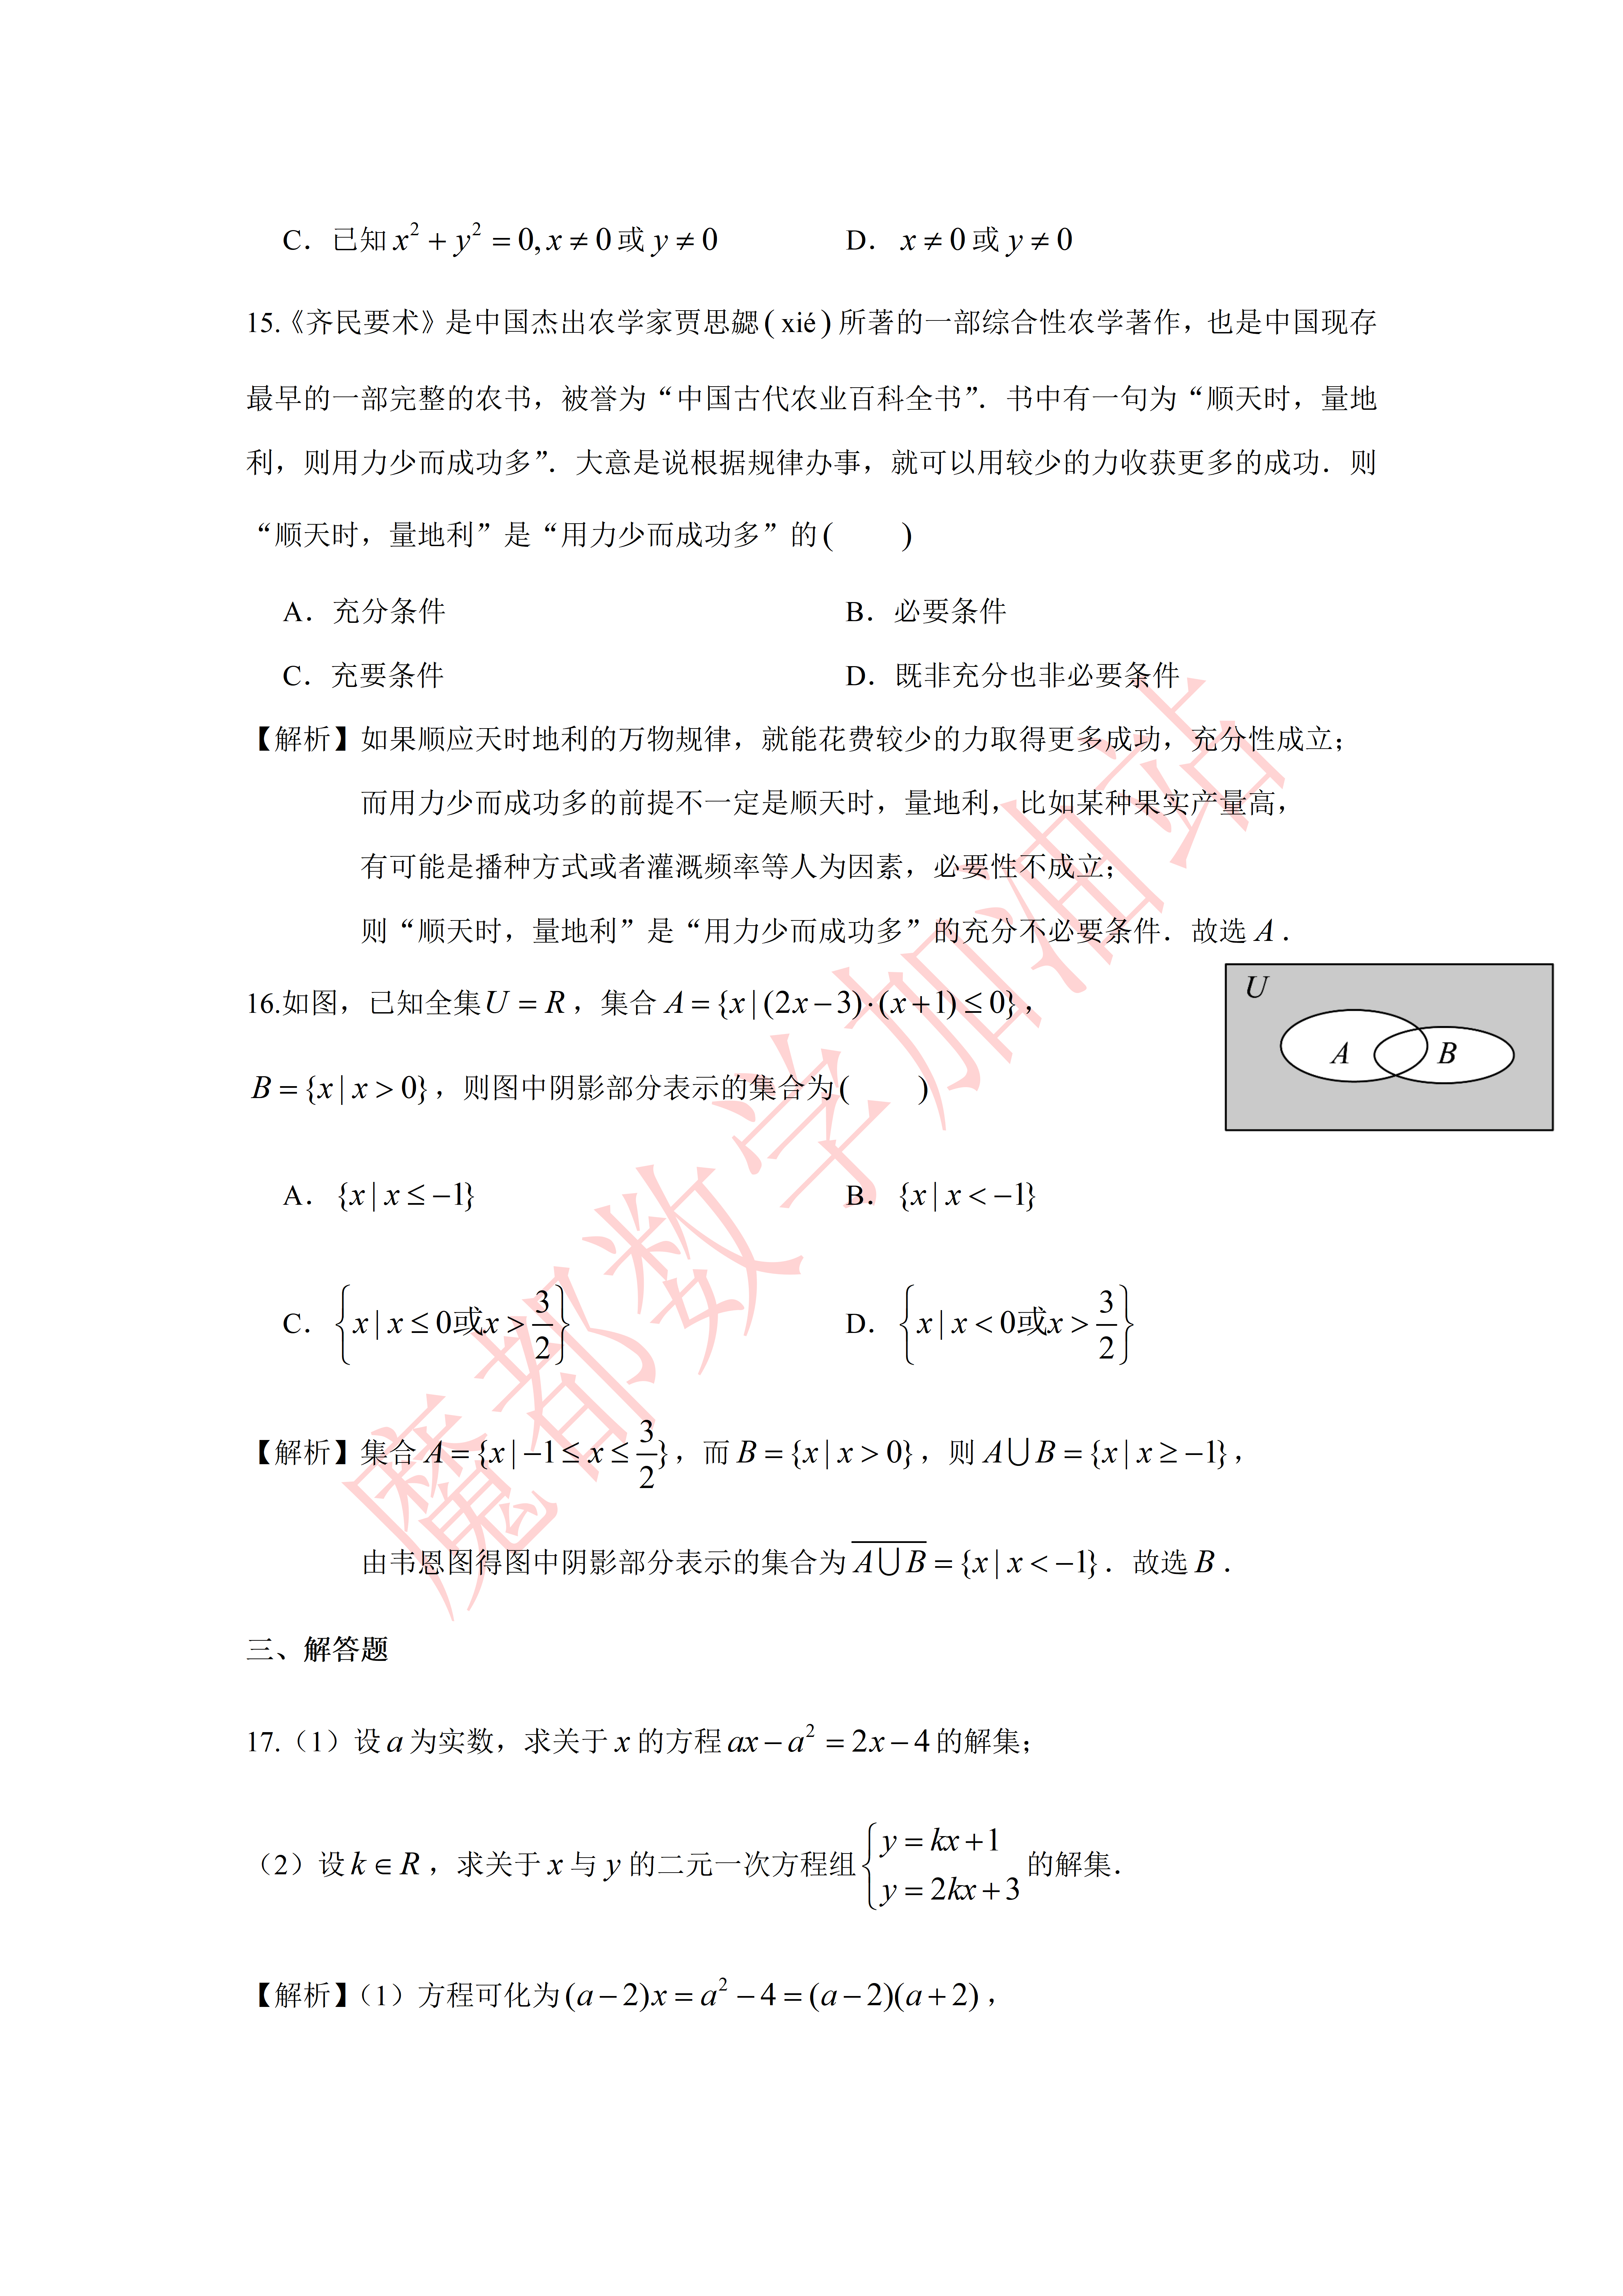
\includegraphics[width=.34\linewidth,trim=3586bp 3410bp 196bp 2818bp,clip]{../原图/高一52_回民中学_9月月考/04.png}
\end{center}

\keepwithprev
A. $\{x\mid x\leqslant-1\}$\qquad B. $\{x\mid x<-1\}$

C. $\left\{x\mid x\leqslant0\text{ 或 }x>\dfrac32\right\}$\qquad D. $\left\{x\mid x<0\text{ 或 }x>\dfrac32\right\}$

\ifanswer
\solbegin
\step{集合 $A=\left\{x\mid-1\leqslant x\leqslant\dfrac32\right\}$，而 $B=\{x\mid x>0\}$，则 $A\cup B=\{x\mid x\geqslant-1\}$，}
\step{由韦恩图得图中阴影部分表示的集合为 $\overline{A\cup B}=\{x\mid x<-1\}$．故选 $B$．}
\solend
\fi

\end{enumerate}

\bigsec{三、解答题}

\begin{enumerate}
\setcounter{enumi}{16}

\item （1）设 $a$ 为实数，求关于 $x$ 的方程 $ax-a^2=2x-4$ 的解集；

（2）设 $k\in\R$，求关于 $x$ 与 $y$ 的二元一次方程组 $\begin{cases}y=kx+1\\y=2kx+3\end{cases}$ 的解集．

\ifanswer
\solbegin
\stepm{(1)}{方程可化为 $(a-2)x=a^2-4=(a-2)(a+2)$，}
\step{当 $a\neq2$ 时，方程的解为 $x=\dfrac{(a-2)(a+2)}{a-2}=a+2$，则解集为 $\{a+2\}$；}
\step{当 $a=2$ 时，方程为 $2x-4=2x-4$，对 $x$ 取一切实数均成立，}
\step{所以解集为 $\R$；}
\stepm{(2)}{$\begin{cases}y=kx+1\\y=2kx+3\end{cases}$，则 $kx+1=2kx+3,kx=-2$，}
\step{当 $k=0$ 时，等式不成立，无解；当 $k\neq0$ 时，$x=-\dfrac2k,y=-1$；}
\step{综上所述，当 $k=0$ 时，解集为 $\varnothing$；当 $k\neq0$ 时，解集为 $\left\{\left(-\dfrac2k,-1\right)\right\}$．}
\solend
\fi

\ansspace[6]

\item 已知命题 $p$：方程 $x^2+6x+m-1=0$ 有两个不等的负根；命题 $q$：方程 $9x^2+6x+m-2=0$ 无实根．

\begin{enumerate}[label=(\arabic*)]
\item 若 $p$ 为真命题，求实数 $m$ 的取值范围；
\item 若 $p,q$ 两命题一真一假，求实数 $m$ 的取值范围．
\end{enumerate}

\ifanswer
\solbegin
\stepm{(1)}{设方程 $x^2+6x+m-1=0$ 两根为 $x_1,x_2$，}
\step{则 $\begin{cases}\Delta>0\\ x_1+x_2<0\\ x_1x_2>0\end{cases}\Rightarrow\begin{cases}36-4(m-1)>0\\ -6<0\\ m-1>0\end{cases}\Rightarrow1<m<10$；}
\stepm{(2)}{若命题 $q$ 为真命题，则 $36-36(m-2)<0\Rightarrow m>3$，}
\step{从而当命题 $q$ 为假命题时，$m\leqslant3$；}
\step{又由（1）得 $p$ 为假命题时，$m\leqslant1$ 或 $m\geqslant10$；}
\step{则当 $p$ 为真命题，$q$ 为假命题时，得 $\begin{cases}1<m<10\\ m\leqslant3\end{cases}\Rightarrow1<m\leqslant3$；}
\step{当 $q$ 为真命题，$p$ 为假命题时，得 $\begin{cases}m\leqslant1\text{ 或 }m\geqslant10\\ m>3\end{cases}\Rightarrow m\geqslant10$；}
\step{综上，当 $p,q$ 两命题一真一假时，$1<m\leqslant3$ 或 $m\geqslant10$.}
\solend
\fi

\ansspace[6]

\item 证明下列两个命题：

\begin{enumerate}[label=(\arabic*)]
\item 设 $ab>0$，求证：$a>b$ 是 $\dfrac1a<\dfrac1b$ 的充要条件．
\item 已知 $a,b$ 为正数，$n$ 为正整数，求证：如果 $a^n>b^n$，那么 $a>b$．
\end{enumerate}

\ifanswer
\solbegin
\stepm{(1)}{先证充分性：因为 $ab>0$ 且 $a>b$，故 $a-b>0$，从而 $\dfrac{a-b}{ab}>0$，}
\step{即 $\dfrac1b-\dfrac1a>0$，即 $\dfrac1a<\dfrac1b$；}
\step{再证必要性：若 $\dfrac1a<\dfrac1b$，则 $\dfrac1a-\dfrac1b=\dfrac{b-a}{ab}<0$，}
\step{又因为 $ab>0$，所以 $b-a<0$，即 $a>b$．}
% 原卷如此，照录未改（第 19 题(1)此句末用全角句号“。”，全卷其余各题末句用“．”，
% 见文件头“原卷笔误/存疑”第 4 条）
\step{综上，$a>b$ 是 $\dfrac1a<\dfrac1b$ 的充要条件。}
\stepm{(2)}{令 $f(x)=x^n,n\in\N^*$，则由幂函数的性质得 $f(x)$ 在第一象限是严格增的，}
\step{而 $a^n>b^n$ 即意味着 $f(a)>f(b)$，且 $a,b$ 为正数，从而 $a>b$．}
\solend
\fi

\ansspace[8]

\item （1）求关于 $x$ 的不等式 $(m-2)x>1-m$ 的解集；

（2）求关于 $x$ 的不等式 $x^2-(a+1)x+a\leqslant0$ 的解集．

\ifanswer
\solbegin
\stepm{(1)}{由不等式 $(m-2)x>1-m$，}
\step{当 $m-2>0$ 时，即 $m>2$ 时，解得 $x>\dfrac{1-m}{m-2}$，}
\step{所以不等式的解集为 $\left(\dfrac{1-m}{m-2},+\infty\right)$；}
\step{当 $m-2=0$ 时，即 $m=2$ 时，不等式即为 $0>-1$ 恒成立，}
\step{即不等式的解集为 $\R$；}
\step{当 $m-2<0$ 时，即 $m<2$ 时，解得 $x<\dfrac{1-m}{m-2}$，}
\step{所以不等式的解集为 $\left(-\infty,\dfrac{1-m}{m-2}\right)$；}
\step{综上，当 $m>2$ 时，解集为 $\left(\dfrac{1-m}{m-2},+\infty\right)$；}
\step{当 $m=2$ 时，解集为 $\R$；}
\step{当 $m<2$ 时，解集为 $\left(-\infty,\dfrac{1-m}{m-2}\right)$．}
\stepm{(2)}{由不等式 $x^2-(a+1)x+a\leqslant0$，可化为 $(x-a)(x-1)\leqslant0$，}
\step{当 $a>1$ 时，解得 $1\leqslant x\leqslant a$，即不等式的解集为 $[1,a]$；}
\step{当 $a=1$ 时，不等式即为 $(x-1)^2\leqslant0$，解得 $x=1$，即不等式的解集为 $\{1\}$；}
\step{当 $a<1$ 时，解得 $a\leqslant x\leqslant1$，即不等式的解集为 $[a,1]$，}
\step{综上，当 $a>1$ 时，解集为 $[1,a]$；}
\step{当 $a=1$ 时，解集为 $\{1\}$；}
\step{当 $a<1$ 时，解集为 $[a,1]$．}
\solend
\fi

\ansspace[10]

\item 已知集合 $A=\{x\mid(x+2)(5-x)\geqslant0\}$，若集合 $B$ 满足 $A\cap B=\varnothing,A\cup B=[-2,7)$．

\begin{enumerate}[label=(\arabic*)]
\item 用区间表示集合 $B$；
\item 若集合 $B$ 是不等式 $-x^2+bx+c>0$ 的解集，求实数 $b,c$ 的值；
\item 已知全集为 $\R$，若关于 $x$ 的不等式 $-1<x-a\leqslant2$ 的解集为 $M$，且“$x\in\overline A$”是“$x\in M$”的必要非充分条件，求实数 $a$ 的取值范围．
\end{enumerate}

\ifanswer
\solbegin
\stepm{(1)}{由题意得 $(x+2)(5-x)\geqslant0\Leftrightarrow(x+2)(x-5)\leqslant0\Rightarrow-2\leqslant x\leqslant5$，}
\step{则 $A=[-2,5]$，又 $A\cap B=\varnothing,A\cup B=[-2,7)$，则 $B=(5,7)$；}
\stepm{(2)}{$-x^2+bx+c>0\Leftrightarrow x^2-bx-c<0$，则 $x^2-bx-c=0$ 两根为 $5,7$，}
\step{则由韦达定理得 $b=12,-c=35\Rightarrow c=-35$；}
\stepm{(3)}{由题意得 $M=(a-1,a+2],\overline A=(-\infty,-2)\cup(5,+\infty)$，}
\step{且“$x\in\overline A$”是“$x\in M$”的必要非充分条件，则 $M$ 是 $\overline A$ 的真子集，}
\step{从而 $a+2<-2$ 或 $a-1\geqslant5$，解得 $a<-4$ 或 $a\geqslant6$，}
\step{所以实数 $a$ 的取值范围为 $(-\infty,-4)\cup[6,+\infty)$．}
\solend
\fi

\ansspace*[10]

\end{enumerate}

\end{document}
"
% 紧凑版：xelatex "\def\iscompact{1}% 高一52_回民中学_9月月考.tex
%   —— 高一上数学“2026-2027 年回民中学高一上 9 月月考”（讲评版）
% 试卷版：xelatex 高一52_回民中学_9月月考.tex
% 答案版：xelatex "\def\isanswer{1}\input{高一52_回民中学_9月月考.tex}"
% 紧凑版：xelatex "\def\iscompact{1}\input{高一52_回民中学_9月月考.tex}"
%
% 原始材料：微信公众号“魔都数学加油站”文章，作者破晓，连载“27学年高一52”；
% 原文标题“27学年高一52——2026-2027年上海市回民中学高一上9月月考”；
% 原文链接：https://mp.weixin.qq.com/s/ndjyozrRQCLl4ba3J8uR7g。
% 该页面用 JS 渲染，未见明确发布日期；页面内时间戳约为 2026-10-06 21:19／21:38，本稿以该时刻记可得日期。
% 正文为 8 张 PNG 页：第 01—07 页 4762×6735，第 08 页 2560×3620（**同一篇各页分辨率不同**），
% 均按页序读取。8 页全为试卷正文页（卷首标题在第 1 页页顶，卷末解答题第 21 题解析止于第 8 页），
% 无封面页、目录页、二维码或宣传页。粉色斜排“魔都数学加油站”为卷面水印，与公众号页脚一并未录入。
%
% 卷首标题：照卷面印作“2026--2027 年回民中学高一上 9 月月考”（公众号标题中的“上海市”
% 卷面标题行没有，本稿照卷面），年份区间按全稿惯例排 en dash。原卷只有一行标题、无副标题。
%
% 篇幅与题号：原卷自第 3 题起编号（第 1、2 题不在本卷内）。填空题 3—12（10 题）、
% 选择题 13—16（4 题）、解答题 17—21（5 题），共 19 题。本稿沿用原节与原题号，
% 只改排为全稿统一的大节样式（原卷小节标题为“一、填空题”“二、选择题”“三、解答题”）。
%
% 讲评版：原卷每题下直接印【答案】或【解析】。**只印【答案】的 1 题**（第 3 题），本稿只给 \ans{}；
% **第 14 题没有任何【答案】/【解析】段**，答案“D”直接印在题干括号内（“应假设(  D  )”），
% 本稿按 高一37 第 13 题的成例把括号留空、答案另提为 \ans{$D$}；
% 其余 17 题都只印【解析】，按全稿口径这类题不另提 \ans{}——其中选择题第 13、15、16 题的结论
% 写在解析末句（“故选 A／A／B”），亦照录在解析内。
%
% 副标题：原卷未印副标题。本稿按“知识模块”口径标作“集合与常用逻辑用语、不等式”：
% 19 题中集合与常用逻辑用语 10 题（集合类 7 题——第 3、4、5、9、12、16、21 题；
% 逻辑类 3 题——第 6、14、15 题），不等式 9 题（含等式性质与一元二次方程：第 7、8、10、11、
% 13、17、18、19、20 题），两类均远超三分之一，故并标。口径同 高一46、高一47、高一48、高一51。
%
% 与原卷的排版差异：
%   ① 原卷每题下直接印【答案】/【解析】，本稿按全稿惯例将答案与解析置于答案版，试卷版保持干净；
%      第 14 题印在题干括号内的答案“D”同样移入 \ans{}，见上；
%   ② 原卷未印副标题，本稿按“知识模块”口径补出；
%   ③ 原卷填空横线约两个字宽，本稿按全稿惯例统一排 \blankline[4.4em]；
%      选择题的作答括号原卷排半角“(    )”，本稿按全稿惯例排 \mbox{（\quad）}；
%   ④ 原卷实数集、自然数集排斜体/粗体 $R$、$\mathbf{R}$、$N$，本稿按全稿惯例改用 $\R$、$\N$；
%      空集记号统一为 \varnothing；
%   ⑤ 第 8 题题干与解析两处“两个实数分别为 $x_1$、$x_2$”原卷即用顿号，第 10、13 题等处
%      原卷在数学式内用半角逗号（如 $x_1,x_2$、$a,b,c\in R$），两份均照录未强改；
%      句末句点按全稿惯例排西文句点，句中句点（第 9、12、15、21 题）照原卷排全角“．”；
%   ⑥ 第 17、20 题原卷把子问标号“（1）”排在该题题号同一行，本稿照原卷仍排同一行（同 高一34 的
%      做法）；第 18、19、21 题的子问原卷各自另起一行，本稿按全稿惯例用 enumerate 的 (1)(2)(3)；
%      解析中的子问标号一律用 \stepm{(1)}{…}；
%   ⑦ 第 16 题的韦恩图原卷排在题干与选项右侧的浮动位置，本稿居中排在题干之后、选项之前，
%      并加 \needvspace 整块推走（守卫写在 \item 之前）；图自原图第 4 页裁切（trim），不另存图片文件；
%   ⑧ 每道解答题原卷未留作答空白，本稿按全稿惯例加 \ansspace。
%
% 原卷笔误/存疑（均照录未改，正文对应处另有 % 注）：
%   1. 第 8 题题干与解析首行两处均作“两个实数分别为 $x_1$、$x_2$”，按文意应为“两个实数**根**”
%      （疑脱“根”字，第 10 题同位置作“两个实根分别是”）；
%   2. 第 4 题解析“满足条件的 $A$ 的个数为集合 $\{0,1,3\}$ 的真子集，即 7 个”，
%      “个数为……真子集”表述不严（应为“……的真子集的个数”）；$\{0,1,3\}$ 的真子集 7 个，结论无误；
%   3. 第 6 题解析第 2 行“当 $a=10,b=0.2$ 时，$a+b>2$，且 $ab>1$，所以 $a>1$，且 $b>1$ 不成立”
%      ——此处是举反例，“所以”按文意应为“但”（$a=10,b=0.2$ 与“$a>1$ 且 $b>1$”不成立之间是转折，
%      非因果）；
%   4. 第 19 题 (1) 解析末行“综上，$a>b$ 是 $\dfrac1a<\dfrac1b$ 的充要条件。”用全角句号“。”，
%      全卷其余各题末句均用“．”，体例不一，照录；
%   5. 第 20 题第 (1) 问解析先按 $m>2$、$m=2$、$m<2$ 三种情况各给出解集，末三行又“综上”重述一遍，
%      与原卷一致（内容重复，非笔误）；
%   6. 第 18 题题干第 (2) 问“若 $p,q$ 两命题一真一假”，正文照录原卷所用半角逗号（未改顿号）。
%
% 插图：1 张，自原图裁切（无 \begin{tikzpicture} 重排）：
%   · 第 16 题题干韦恩图（全集 $U$ 矩形内两相交椭圆 $A$、$B$，灰色为阴影部分）
%     ——原图第 04 页，原卷排于题干与选项右侧。
%     裁框：x 3594–4558、y 2826–3317（即矩形外框，四周各留 4px），
%     trim=3590bp 3414bp 200bp 2822bp（左／下／右／上），页宽 4762、页高 6735。
%
\documentclass[a4paper,11pt]{article}
\usepackage{common}

\begin{document}

\examtitlest[3]{2026--2027 年回民中学高一上 9 月月考}{集合与常用逻辑用语、不等式}

\bigsec{一、填空题}

\begin{enumerate}
\setcounter{enumi}{2}

\item 用列举法写出下列集合 $\{(x,y)\mid x+y=2,x\in\N,y\in\N\}=$\blankline[4.4em].

\ifanswer
\ans{$\{(0,2),(1,1),(2,0)\}$}
\fi

\item 设集合 $A$ 满足 $\{-1,2\}\sub A\subset\{-1,0,1,2,3\}$，则满足条件的 $A$ 有\blankline[4.4em]个.

\ifanswer
\solbegin
\step{满足条件的 $A$ 的个数为集合 $\{0,1,3\}$ 的真子集，即 $7$ 个.}
\solend
\fi

\item 已知集合 $A=\{2,(a+1)^2,a^2+2\}$，且 $1\in A$，则实数 $a$ 的值为\blankline[4.4em].

\ifanswer
\solbegin
\step{因为 $1\in A$，而 $a^2+2\geqslant2$，所以 $(a+1)^2=1$，解得 $a=0$ 或 $a=-2$，}
\step{$a=0$ 时，$a^2+2=2$，不合题意，$a=-2$ 时，$a^2+2=6$，满足题意，}
\step{所以 $a=-2$.}
\solend
\fi

\item 已知 $a,b$ 是实数，则“$a>1$，且 $b>1$”是“$a+b>2$，且 $ab>1$”的\blankline[4.4em]条件.

\ifanswer
\solbegin
\step{$a,b$ 是实数，则“$a>1$，且 $b>1$”$\Rightarrow$“$a+b>2$，且 $ab>1$”正确，}
% 原卷如此，照录未改（第 6 题解析此处作“所以 $a>1$，且 $b>1$ 不成立”，按文意为转折，
% 见文件头“原卷笔误/存疑”第 3 条）
\step{当 $a=10,b=0.2$ 时，$a+b>2$，且 $ab>1$，所以 $a>1$，且 $b>1$ 不成立，}
\step{即前者是推出后者，后者推不出前者，}
\step{所以“$a>1$，且 $b>1$”是“$a+b>2$，且 $ab>1$”的充分而不必要条件.}
\solend
\fi

\item 已知等式 $2x^2-3x-1=a(x-1)^2+b(x-1)+c$ 恒成立，其中 $a,b,c$ 为常数，则 $a+b-c=$\blankline[4.4em].

\ifanswer
\solbegin
\step{将等式右侧展开整理得 $a(x-1)^2+b(x-1)+c=ax^2+(-2a+b)x+(a-b+c)$，}
\step{左右两边多项式恒等，对应次数的系数必须相等：}
\step{则 $a=2,-2a+b=-3$，代入 $a=2$ 得 $b=1$，$a-b+c=-1$，}
\step{代入 $a=2,b=1$ 得 $c=-2$，得 $a+b-c=2+1-(-2)=5$.}
\solend
\fi

% 原卷如此，照录未改（第 8 题题干与解析首行两处“两个实数分别为”疑脱“根”字，
% 见文件头“原卷笔误/存疑”第 1 条）
\item 若关于 $x$ 的二次方程 $x^2+mx+4m^2-3=0$ 的两个实数分别为 $x_1$、$x_2$，且满足 $x_1+x_2=x_1x_2$，则实数 $m$ 的值为\blankline[4.4em].

\ifanswer
\solbegin
% 原卷如此，照录未改（此处“两个实数分别为”同题干，疑脱“根”字）
\step{二次方程 $x^2+mx+4m^2-3=0$ 的两个实数分别为 $x_1$、$x_2$，}
\step{则有 $\Delta=m^2-4(4m^2-3)\geqslant0$，变形得 $m^2\leqslant\dfrac45$，}
\step{则 $x_1+x_2=-m$，$x_1x_2=(4m^2-3)$，}
\step{若 $x_1+x_2=x_1x_2$，则有 $-m=4m^2-3$，解得 $m=-1$ 或 $\dfrac34$，}
\step{又 $m^2\leqslant\dfrac45$，则 $m=\dfrac34$.}
\solend
\fi

\item 设集合 $A=\{x\mid x^2=1\}$，$B=\{x\mid ax=1\}$．若 $A\cap B=B$，则实数 $a$ 的值为\blankline[4.4em].

\ifanswer
\solbegin
\step{集合 $A=\{x\mid x^2=1\}=\{-1,1\}$，$B=\{x\mid ax=1\}$，$A\cap B=B$，所以 $B\sub A$，}
\step{当 $a=0$ 时，$B=\varnothing$，成立；}
\step{当 $a\neq0$ 时，$B=\left\{\dfrac1a\right\}$，则 $\dfrac1a=-1$ 或 $\dfrac1a=1$，解得 $a=-1$ 或 $a=1$，}
\step{所以实数 $a$ 的值为 $0$ 或 $1$ 或 $-1$.}
\solend
\fi

\item 已知关于 $x$ 的一元二次方程 $x^2+3x-3=0$ 的两个实根分别是 $x_1,x_2$，则以 $-\dfrac1{x_1},-\dfrac1{x_2}$ 为根且二次项系数是 $1$ 的一元二次方程为\blankline[4.4em].

\ifanswer
\solbegin
\step{因为 $x_1,x_2$ 是一元二次方程 $x^2+3x-3=0$ 的两个实根，}
\step{所以 $x_1+x_2=-3,x_1x_2=-3$，}
\step{所以 $-\dfrac1{x_1}+\left(-\dfrac1{x_2}\right)=-\dfrac{x_1+x_2}{x_1x_2}=-1$，$-\dfrac1{x_1}\cdot\left(-\dfrac1{x_2}\right)=\dfrac1{x_1x_2}=-\dfrac13$，}
\step{所以一元二次方程为 $x^2+x-\dfrac13=0$.}
\solend
\fi

\item 若关于 $x$ 的不等式 $(a-2)x^2+2(a-2)x-4<0$ 的解集是 $\R$，则实数 $a$ 的取值范围是\blankline[4.4em].

\ifanswer
\solbegin
\step{当 $a=2$ 时，不等式化为 $-4<0$ 对于任意实数 $x$ 都成立，因此 $a=2$ 满足题意；}
\step{当 $a\neq2$ 时，要使关于 $x$ 的不等式 $(a-2)x^2+2(a-2)x-4<0$ 的解集为 $\R$，}
\step{则 $\begin{cases}a-2<0\\ \Delta=4(a-2)^2+16(a-2)<0\end{cases}$，解得 $-2<a<2$．}
\step{综上，$a$ 的取值范围为 $(-2,2]$．}
\solend
\fi

\item 设非空集合 $A$、$B$，定义 $A\times B=\{x\mid x\in(A\cup B),x\notin(A\cap B)\}$．已知 $A=\{x\mid0\leqslant x\leqslant2\}$，$B=\{y\mid y\geqslant0\}$，则 $A\times B=$\blankline[4.4em].

\ifanswer
\solbegin
\step{由于 $A=\{x\mid0\leqslant x\leqslant2\}$，$B=\{y\mid y\geqslant0\}=\{x\mid x\geqslant0\}$，}
\step{所以 $A\cup B=\{x\mid x\geqslant0\}$，$A\cap B=\{x\mid0\leqslant x\leqslant2\}$，故 $A\times B=\{x\mid x>2\}$．}
\solend
\fi

\end{enumerate}

\bigsec{二、选择题}

\begin{enumerate}
\setcounter{enumi}{12}

\item 已知 $a,b,c\in\R$ 且 $a>b$，则下列不等式一定成立的是\mbox{（\quad）}

\keepwithprev
A. $\dfrac{a}{c^2+1}>\dfrac{b}{c^2+1}$\qquad B. $\dfrac1a<\dfrac1b$

C. $ac>bc$\qquad D. $a^2>b^2$

\ifanswer
\solbegin
\step{对于 A：因为 $c^2+1>0$ 恒成立，且 $a>b$，所以 $\dfrac{a}{c^2+1}>\dfrac{b}{c^2+1}$ 一定成立，}
\step{所以 A 正确；}
\step{对于 B：当 $a=1,b=-1$ 时，满足 $a>b$，此时 $\dfrac1a=1>\dfrac1b=-1$，所以 B 错误；}
\step{对于 C：当 $c<0$ 时，由 $a>b$，得 $ac<bc$，所以 C 错误；}
\step{对于 D：当 $a=1,b=-2$ 时，满足 $a>b$，此时 $a^2=1<b^2=4$，所以 D 错误；}
\step{故选 $A$．}
\solend
\fi

% 注：本题的答案“D”原卷直接印在题干末尾的括号内（“应假设(  D  )”），且没有单独的
%     【答案】/【解析】段，本稿按 高一37 第 13 题的成例把括号留空、另提为 \ans{}，
%     见文件头“与原卷的排版差异”①。
\item 用反证法证明：“已知 $x,y\in\R$,$x^2+y^2=0$，求证：$x=y=0$”时，应假设\mbox{（\quad）}

\keepwithprev
A. 已知 $x^2+y^2=0,x\neq0$ 且 $y\neq0$\qquad B. $x\neq0$ 且 $y\neq0$

C. 已知 $x^2+y^2=0,x\neq0$ 或 $y\neq0$\qquad D. $x\neq0$ 或 $y\neq0$

\ans{$D$}

\item 《齐民要术》是中国杰出农学家贾思勰（xié）所著的一部综合性农学著作，也是中国现存最早的一部完整的农书，被誉为“中国古代农业百科全书”．书中有一句为“顺天时，量地利，则用力少而成功多”．大意是说根据规律办事，就可以用较少的力收获更多的成功．则“顺天时，量地利”是“用力少而成功多”的\mbox{（\quad）}

\keepwithprev
A. 充分条件\qquad B. 必要条件

C. 充要条件\qquad D. 既非充分也非必要条件

\ifanswer
\solbegin
\step{如果顺应天时地利的万物规律，就能花费较少的力取得更多成功，充分性成立；}
\step{而用力少而成功多的前提不一定是顺天时，量地利，比如某种果实产量高，}
\step{有可能是播种方式或者灌溉频率等人为因素，必要性不成立；}
\step{则“顺天时，量地利”是“用力少而成功多”的充分不必要条件．故选 $A$．}
\solend
\fi

\needvspace{13\baselineskip}

\item 如图，已知全集 $U=\R$，集合 $A=\{x\mid(2x-3)\cdot(x+1)\leqslant0\}$，$B=\{x\mid x>0\}$，则图中阴影部分表示的集合为\mbox{（\quad）}

\begin{center}
% 原图第 4 页题干韦恩图直接裁取（原卷排于题干与选项右侧）。
% 裁框取矩形外框 x 3590–4558、y 2822–3321，再向外各留 4px（即 x 3586–4562、y 2818–3325），
% trim=左 3586bp／下 3410bp／右 196bp／上 2818bp（页宽 4762、页高 6735）。
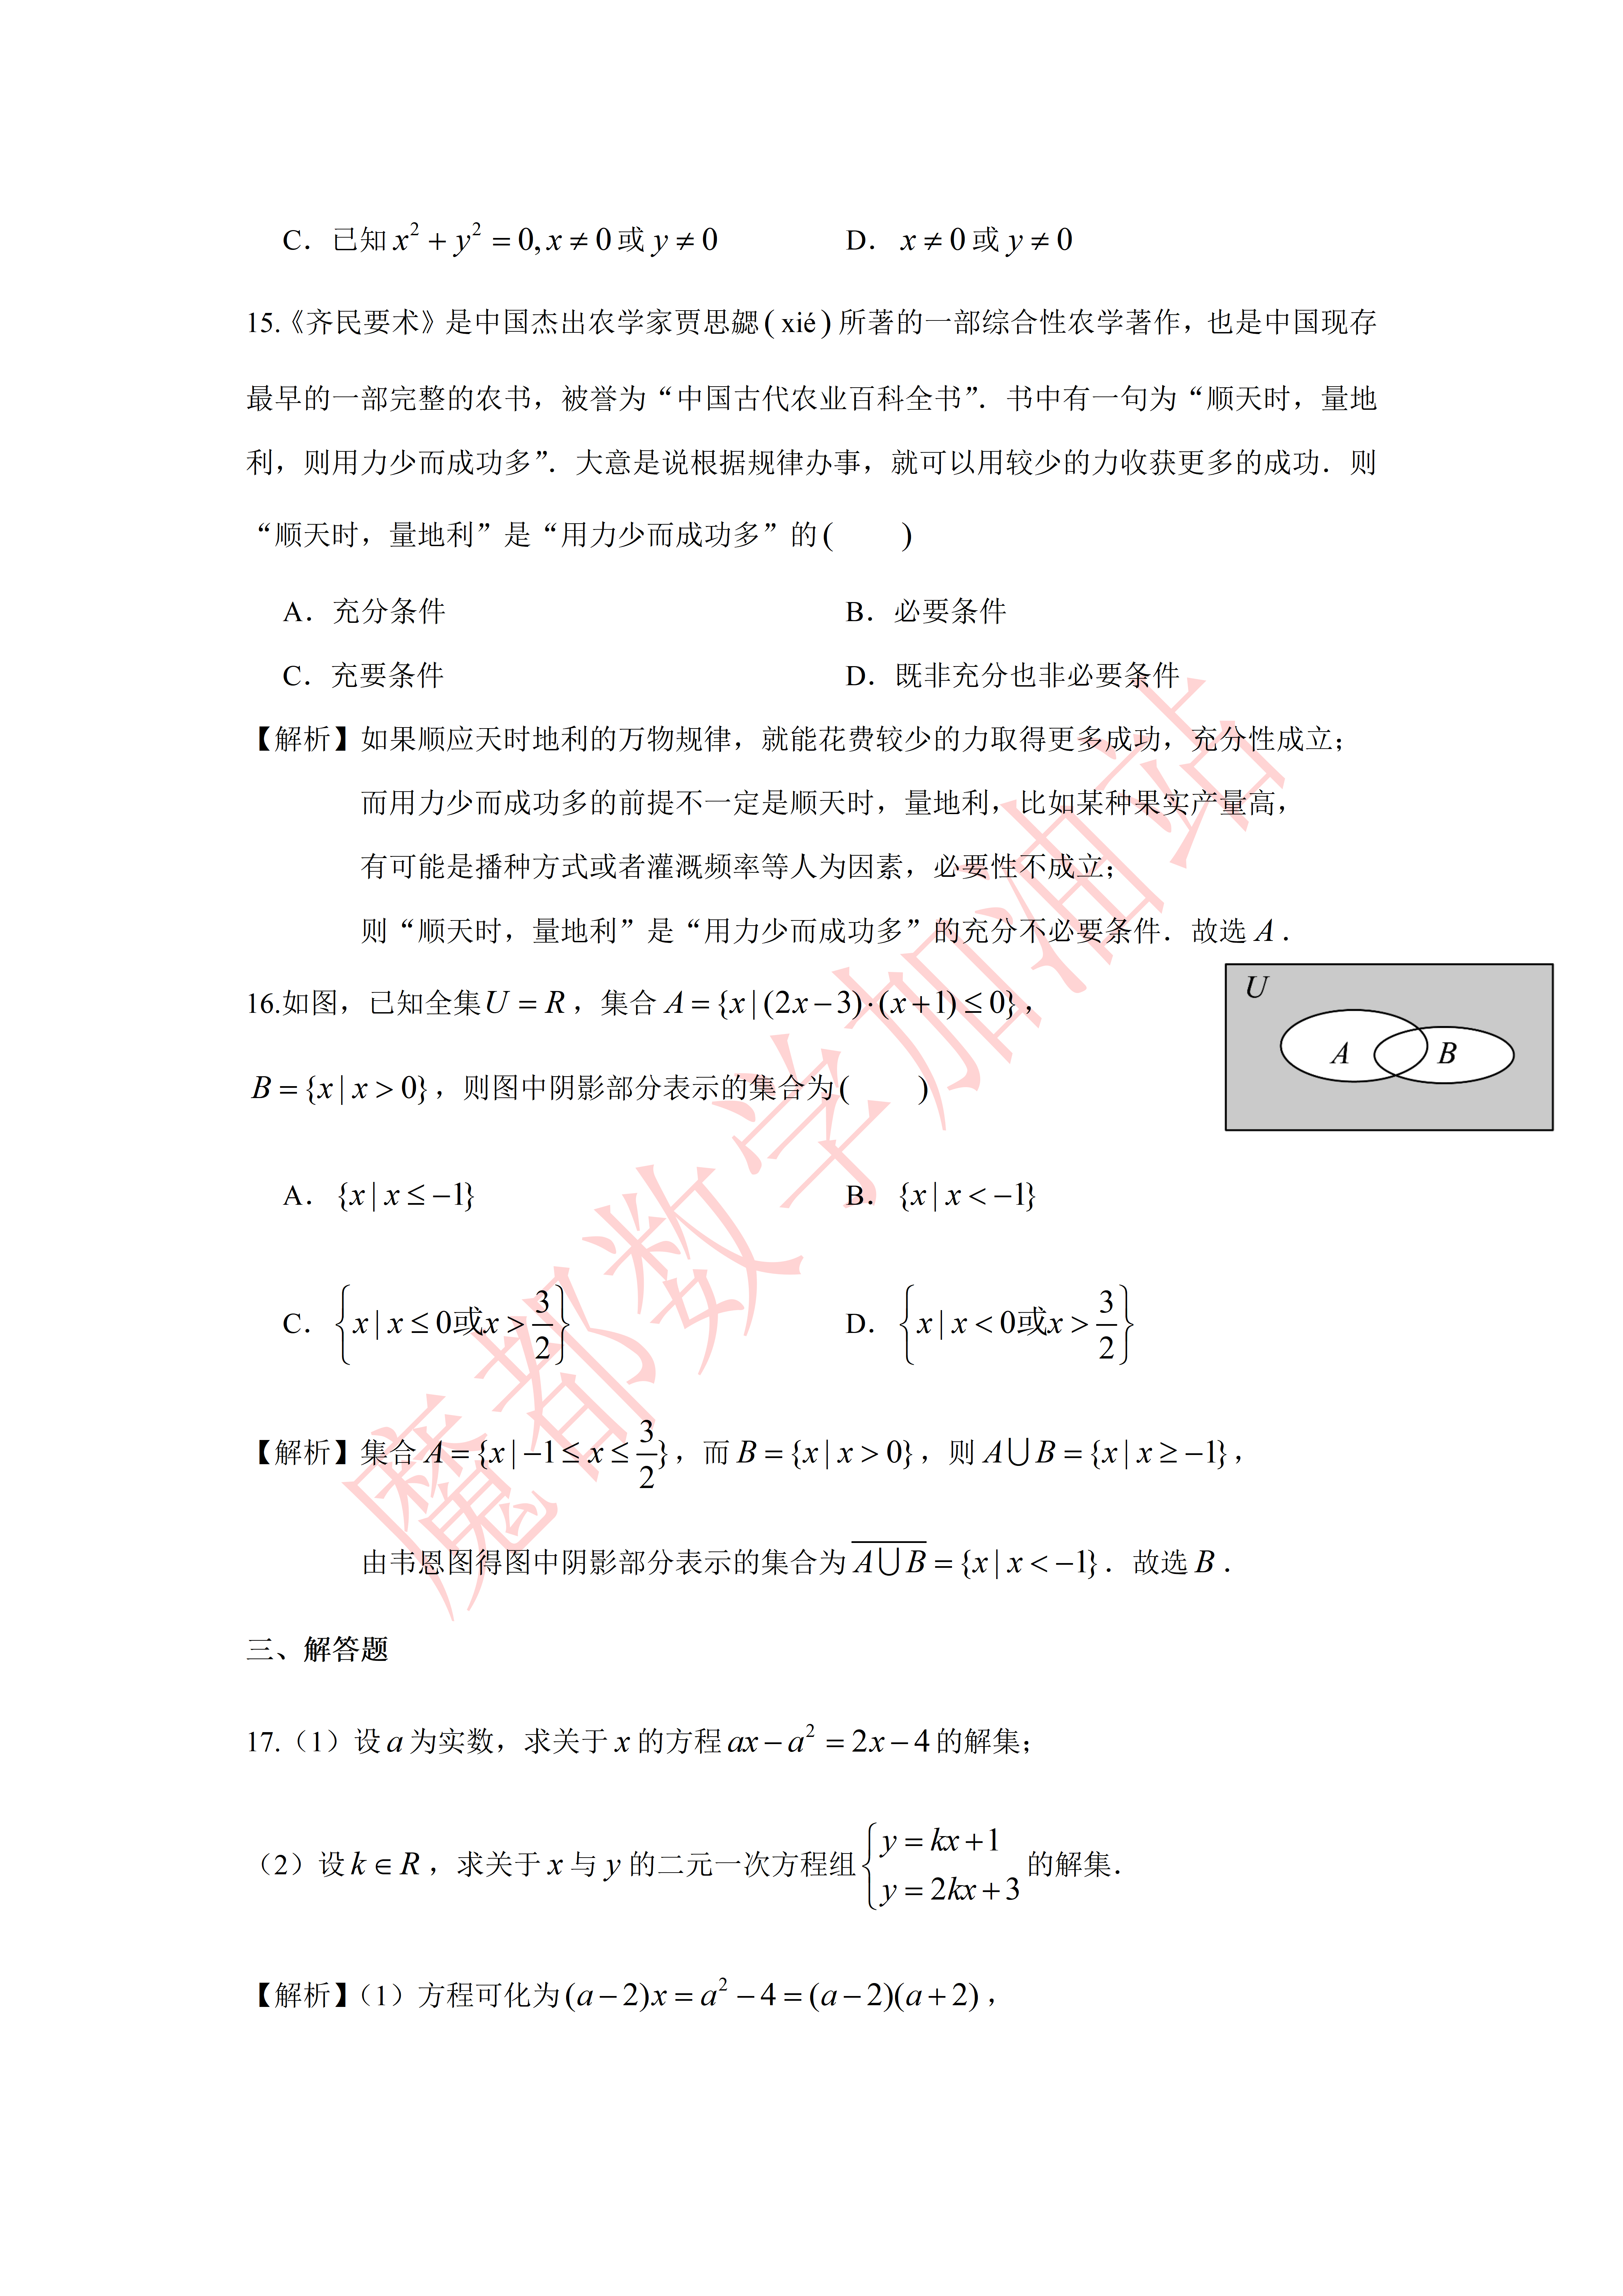
\includegraphics[width=.34\linewidth,trim=3586bp 3410bp 196bp 2818bp,clip]{../原图/高一52_回民中学_9月月考/04.png}
\end{center}

\keepwithprev
A. $\{x\mid x\leqslant-1\}$\qquad B. $\{x\mid x<-1\}$

C. $\left\{x\mid x\leqslant0\text{ 或 }x>\dfrac32\right\}$\qquad D. $\left\{x\mid x<0\text{ 或 }x>\dfrac32\right\}$

\ifanswer
\solbegin
\step{集合 $A=\left\{x\mid-1\leqslant x\leqslant\dfrac32\right\}$，而 $B=\{x\mid x>0\}$，则 $A\cup B=\{x\mid x\geqslant-1\}$，}
\step{由韦恩图得图中阴影部分表示的集合为 $\overline{A\cup B}=\{x\mid x<-1\}$．故选 $B$．}
\solend
\fi

\end{enumerate}

\bigsec{三、解答题}

\begin{enumerate}
\setcounter{enumi}{16}

\item （1）设 $a$ 为实数，求关于 $x$ 的方程 $ax-a^2=2x-4$ 的解集；

（2）设 $k\in\R$，求关于 $x$ 与 $y$ 的二元一次方程组 $\begin{cases}y=kx+1\\y=2kx+3\end{cases}$ 的解集．

\ifanswer
\solbegin
\stepm{(1)}{方程可化为 $(a-2)x=a^2-4=(a-2)(a+2)$，}
\step{当 $a\neq2$ 时，方程的解为 $x=\dfrac{(a-2)(a+2)}{a-2}=a+2$，则解集为 $\{a+2\}$；}
\step{当 $a=2$ 时，方程为 $2x-4=2x-4$，对 $x$ 取一切实数均成立，}
\step{所以解集为 $\R$；}
\stepm{(2)}{$\begin{cases}y=kx+1\\y=2kx+3\end{cases}$，则 $kx+1=2kx+3,kx=-2$，}
\step{当 $k=0$ 时，等式不成立，无解；当 $k\neq0$ 时，$x=-\dfrac2k,y=-1$；}
\step{综上所述，当 $k=0$ 时，解集为 $\varnothing$；当 $k\neq0$ 时，解集为 $\left\{\left(-\dfrac2k,-1\right)\right\}$．}
\solend
\fi

\ansspace[6]

\item 已知命题 $p$：方程 $x^2+6x+m-1=0$ 有两个不等的负根；命题 $q$：方程 $9x^2+6x+m-2=0$ 无实根．

\begin{enumerate}[label=(\arabic*)]
\item 若 $p$ 为真命题，求实数 $m$ 的取值范围；
\item 若 $p,q$ 两命题一真一假，求实数 $m$ 的取值范围．
\end{enumerate}

\ifanswer
\solbegin
\stepm{(1)}{设方程 $x^2+6x+m-1=0$ 两根为 $x_1,x_2$，}
\step{则 $\begin{cases}\Delta>0\\ x_1+x_2<0\\ x_1x_2>0\end{cases}\Rightarrow\begin{cases}36-4(m-1)>0\\ -6<0\\ m-1>0\end{cases}\Rightarrow1<m<10$；}
\stepm{(2)}{若命题 $q$ 为真命题，则 $36-36(m-2)<0\Rightarrow m>3$，}
\step{从而当命题 $q$ 为假命题时，$m\leqslant3$；}
\step{又由（1）得 $p$ 为假命题时，$m\leqslant1$ 或 $m\geqslant10$；}
\step{则当 $p$ 为真命题，$q$ 为假命题时，得 $\begin{cases}1<m<10\\ m\leqslant3\end{cases}\Rightarrow1<m\leqslant3$；}
\step{当 $q$ 为真命题，$p$ 为假命题时，得 $\begin{cases}m\leqslant1\text{ 或 }m\geqslant10\\ m>3\end{cases}\Rightarrow m\geqslant10$；}
\step{综上，当 $p,q$ 两命题一真一假时，$1<m\leqslant3$ 或 $m\geqslant10$.}
\solend
\fi

\ansspace[6]

\item 证明下列两个命题：

\begin{enumerate}[label=(\arabic*)]
\item 设 $ab>0$，求证：$a>b$ 是 $\dfrac1a<\dfrac1b$ 的充要条件．
\item 已知 $a,b$ 为正数，$n$ 为正整数，求证：如果 $a^n>b^n$，那么 $a>b$．
\end{enumerate}

\ifanswer
\solbegin
\stepm{(1)}{先证充分性：因为 $ab>0$ 且 $a>b$，故 $a-b>0$，从而 $\dfrac{a-b}{ab}>0$，}
\step{即 $\dfrac1b-\dfrac1a>0$，即 $\dfrac1a<\dfrac1b$；}
\step{再证必要性：若 $\dfrac1a<\dfrac1b$，则 $\dfrac1a-\dfrac1b=\dfrac{b-a}{ab}<0$，}
\step{又因为 $ab>0$，所以 $b-a<0$，即 $a>b$．}
% 原卷如此，照录未改（第 19 题(1)此句末用全角句号“。”，全卷其余各题末句用“．”，
% 见文件头“原卷笔误/存疑”第 4 条）
\step{综上，$a>b$ 是 $\dfrac1a<\dfrac1b$ 的充要条件。}
\stepm{(2)}{令 $f(x)=x^n,n\in\N^*$，则由幂函数的性质得 $f(x)$ 在第一象限是严格增的，}
\step{而 $a^n>b^n$ 即意味着 $f(a)>f(b)$，且 $a,b$ 为正数，从而 $a>b$．}
\solend
\fi

\ansspace[8]

\item （1）求关于 $x$ 的不等式 $(m-2)x>1-m$ 的解集；

（2）求关于 $x$ 的不等式 $x^2-(a+1)x+a\leqslant0$ 的解集．

\ifanswer
\solbegin
\stepm{(1)}{由不等式 $(m-2)x>1-m$，}
\step{当 $m-2>0$ 时，即 $m>2$ 时，解得 $x>\dfrac{1-m}{m-2}$，}
\step{所以不等式的解集为 $\left(\dfrac{1-m}{m-2},+\infty\right)$；}
\step{当 $m-2=0$ 时，即 $m=2$ 时，不等式即为 $0>-1$ 恒成立，}
\step{即不等式的解集为 $\R$；}
\step{当 $m-2<0$ 时，即 $m<2$ 时，解得 $x<\dfrac{1-m}{m-2}$，}
\step{所以不等式的解集为 $\left(-\infty,\dfrac{1-m}{m-2}\right)$；}
\step{综上，当 $m>2$ 时，解集为 $\left(\dfrac{1-m}{m-2},+\infty\right)$；}
\step{当 $m=2$ 时，解集为 $\R$；}
\step{当 $m<2$ 时，解集为 $\left(-\infty,\dfrac{1-m}{m-2}\right)$．}
\stepm{(2)}{由不等式 $x^2-(a+1)x+a\leqslant0$，可化为 $(x-a)(x-1)\leqslant0$，}
\step{当 $a>1$ 时，解得 $1\leqslant x\leqslant a$，即不等式的解集为 $[1,a]$；}
\step{当 $a=1$ 时，不等式即为 $(x-1)^2\leqslant0$，解得 $x=1$，即不等式的解集为 $\{1\}$；}
\step{当 $a<1$ 时，解得 $a\leqslant x\leqslant1$，即不等式的解集为 $[a,1]$，}
\step{综上，当 $a>1$ 时，解集为 $[1,a]$；}
\step{当 $a=1$ 时，解集为 $\{1\}$；}
\step{当 $a<1$ 时，解集为 $[a,1]$．}
\solend
\fi

\ansspace[10]

\item 已知集合 $A=\{x\mid(x+2)(5-x)\geqslant0\}$，若集合 $B$ 满足 $A\cap B=\varnothing,A\cup B=[-2,7)$．

\begin{enumerate}[label=(\arabic*)]
\item 用区间表示集合 $B$；
\item 若集合 $B$ 是不等式 $-x^2+bx+c>0$ 的解集，求实数 $b,c$ 的值；
\item 已知全集为 $\R$，若关于 $x$ 的不等式 $-1<x-a\leqslant2$ 的解集为 $M$，且“$x\in\overline A$”是“$x\in M$”的必要非充分条件，求实数 $a$ 的取值范围．
\end{enumerate}

\ifanswer
\solbegin
\stepm{(1)}{由题意得 $(x+2)(5-x)\geqslant0\Leftrightarrow(x+2)(x-5)\leqslant0\Rightarrow-2\leqslant x\leqslant5$，}
\step{则 $A=[-2,5]$，又 $A\cap B=\varnothing,A\cup B=[-2,7)$，则 $B=(5,7)$；}
\stepm{(2)}{$-x^2+bx+c>0\Leftrightarrow x^2-bx-c<0$，则 $x^2-bx-c=0$ 两根为 $5,7$，}
\step{则由韦达定理得 $b=12,-c=35\Rightarrow c=-35$；}
\stepm{(3)}{由题意得 $M=(a-1,a+2],\overline A=(-\infty,-2)\cup(5,+\infty)$，}
\step{且“$x\in\overline A$”是“$x\in M$”的必要非充分条件，则 $M$ 是 $\overline A$ 的真子集，}
\step{从而 $a+2<-2$ 或 $a-1\geqslant5$，解得 $a<-4$ 或 $a\geqslant6$，}
\step{所以实数 $a$ 的取值范围为 $(-\infty,-4)\cup[6,+\infty)$．}
\solend
\fi

\ansspace*[10]

\end{enumerate}

\end{document}
"
%
% 原始材料：微信公众号“魔都数学加油站”文章，作者破晓，连载“27学年高一52”；
% 原文标题“27学年高一52——2026-2027年上海市回民中学高一上9月月考”；
% 原文链接：https://mp.weixin.qq.com/s/ndjyozrRQCLl4ba3J8uR7g。
% 该页面用 JS 渲染，未见明确发布日期；页面内时间戳约为 2026-10-06 21:19／21:38，本稿以该时刻记可得日期。
% 正文为 8 张 PNG 页：第 01—07 页 4762×6735，第 08 页 2560×3620（**同一篇各页分辨率不同**），
% 均按页序读取。8 页全为试卷正文页（卷首标题在第 1 页页顶，卷末解答题第 21 题解析止于第 8 页），
% 无封面页、目录页、二维码或宣传页。粉色斜排“魔都数学加油站”为卷面水印，与公众号页脚一并未录入。
%
% 卷首标题：照卷面印作“2026--2027 年回民中学高一上 9 月月考”（公众号标题中的“上海市”
% 卷面标题行没有，本稿照卷面），年份区间按全稿惯例排 en dash。原卷只有一行标题、无副标题。
%
% 篇幅与题号：原卷自第 3 题起编号（第 1、2 题不在本卷内）。填空题 3—12（10 题）、
% 选择题 13—16（4 题）、解答题 17—21（5 题），共 19 题。本稿沿用原节与原题号，
% 只改排为全稿统一的大节样式（原卷小节标题为“一、填空题”“二、选择题”“三、解答题”）。
%
% 讲评版：原卷每题下直接印【答案】或【解析】。**只印【答案】的 1 题**（第 3 题），本稿只给 \ans{}；
% **第 14 题没有任何【答案】/【解析】段**，答案“D”直接印在题干括号内（“应假设(  D  )”），
% 本稿按 高一37 第 13 题的成例把括号留空、答案另提为 \ans{$D$}；
% 其余 17 题都只印【解析】，按全稿口径这类题不另提 \ans{}——其中选择题第 13、15、16 题的结论
% 写在解析末句（“故选 A／A／B”），亦照录在解析内。
%
% 副标题：原卷未印副标题。本稿按“知识模块”口径标作“集合与常用逻辑用语、不等式”：
% 19 题中集合与常用逻辑用语 10 题（集合类 7 题——第 3、4、5、9、12、16、21 题；
% 逻辑类 3 题——第 6、14、15 题），不等式 9 题（含等式性质与一元二次方程：第 7、8、10、11、
% 13、17、18、19、20 题），两类均远超三分之一，故并标。口径同 高一46、高一47、高一48、高一51。
%
% 与原卷的排版差异：
%   ① 原卷每题下直接印【答案】/【解析】，本稿按全稿惯例将答案与解析置于答案版，试卷版保持干净；
%      第 14 题印在题干括号内的答案“D”同样移入 \ans{}，见上；
%   ② 原卷未印副标题，本稿按“知识模块”口径补出；
%   ③ 原卷填空横线约两个字宽，本稿按全稿惯例统一排 \blankline[4.4em]；
%      选择题的作答括号原卷排半角“(    )”，本稿按全稿惯例排 \mbox{（\quad）}；
%   ④ 原卷实数集、自然数集排斜体/粗体 $R$、$\mathbf{R}$、$N$，本稿按全稿惯例改用 $\R$、$\N$；
%      空集记号统一为 \varnothing；
%   ⑤ 第 8 题题干与解析两处“两个实数分别为 $x_1$、$x_2$”原卷即用顿号，第 10、13 题等处
%      原卷在数学式内用半角逗号（如 $x_1,x_2$、$a,b,c\in R$），两份均照录未强改；
%      句末句点按全稿惯例排西文句点，句中句点（第 9、12、15、21 题）照原卷排全角“．”；
%   ⑥ 第 17、20 题原卷把子问标号“（1）”排在该题题号同一行，本稿照原卷仍排同一行（同 高一34 的
%      做法）；第 18、19、21 题的子问原卷各自另起一行，本稿按全稿惯例用 enumerate 的 (1)(2)(3)；
%      解析中的子问标号一律用 \stepm{(1)}{…}；
%   ⑦ 第 16 题的韦恩图原卷排在题干与选项右侧的浮动位置，本稿居中排在题干之后、选项之前，
%      并加 \needvspace 整块推走（守卫写在 \item 之前）；图自原图第 4 页裁切（trim），不另存图片文件；
%   ⑧ 每道解答题原卷未留作答空白，本稿按全稿惯例加 \ansspace。
%
% 原卷笔误/存疑（均照录未改，正文对应处另有 % 注）：
%   1. 第 8 题题干与解析首行两处均作“两个实数分别为 $x_1$、$x_2$”，按文意应为“两个实数**根**”
%      （疑脱“根”字，第 10 题同位置作“两个实根分别是”）；
%   2. 第 4 题解析“满足条件的 $A$ 的个数为集合 $\{0,1,3\}$ 的真子集，即 7 个”，
%      “个数为……真子集”表述不严（应为“……的真子集的个数”）；$\{0,1,3\}$ 的真子集 7 个，结论无误；
%   3. 第 6 题解析第 2 行“当 $a=10,b=0.2$ 时，$a+b>2$，且 $ab>1$，所以 $a>1$，且 $b>1$ 不成立”
%      ——此处是举反例，“所以”按文意应为“但”（$a=10,b=0.2$ 与“$a>1$ 且 $b>1$”不成立之间是转折，
%      非因果）；
%   4. 第 19 题 (1) 解析末行“综上，$a>b$ 是 $\dfrac1a<\dfrac1b$ 的充要条件。”用全角句号“。”，
%      全卷其余各题末句均用“．”，体例不一，照录；
%   5. 第 20 题第 (1) 问解析先按 $m>2$、$m=2$、$m<2$ 三种情况各给出解集，末三行又“综上”重述一遍，
%      与原卷一致（内容重复，非笔误）；
%   6. 第 18 题题干第 (2) 问“若 $p,q$ 两命题一真一假”，正文照录原卷所用半角逗号（未改顿号）。
%
% 插图：1 张，自原图裁切（无 \begin{tikzpicture} 重排）：
%   · 第 16 题题干韦恩图（全集 $U$ 矩形内两相交椭圆 $A$、$B$，灰色为阴影部分）
%     ——原图第 04 页，原卷排于题干与选项右侧。
%     裁框：x 3594–4558、y 2826–3317（即矩形外框，四周各留 4px），
%     trim=3590bp 3414bp 200bp 2822bp（左／下／右／上），页宽 4762、页高 6735。
%
\documentclass[a4paper,11pt]{article}
\usepackage{common}

\begin{document}

\examtitlest[3]{2026--2027 年回民中学高一上 9 月月考}{集合与常用逻辑用语、不等式}

\bigsec{一、填空题}

\begin{enumerate}
\setcounter{enumi}{2}

\item 用列举法写出下列集合 $\{(x,y)\mid x+y=2,x\in\N,y\in\N\}=$\blankline[4.4em].

\ifanswer
\ans{$\{(0,2),(1,1),(2,0)\}$}
\fi

\item 设集合 $A$ 满足 $\{-1,2\}\sub A\subset\{-1,0,1,2,3\}$，则满足条件的 $A$ 有\blankline[4.4em]个.

\ifanswer
\solbegin
\step{满足条件的 $A$ 的个数为集合 $\{0,1,3\}$ 的真子集，即 $7$ 个.}
\solend
\fi

\item 已知集合 $A=\{2,(a+1)^2,a^2+2\}$，且 $1\in A$，则实数 $a$ 的值为\blankline[4.4em].

\ifanswer
\solbegin
\step{因为 $1\in A$，而 $a^2+2\geqslant2$，所以 $(a+1)^2=1$，解得 $a=0$ 或 $a=-2$，}
\step{$a=0$ 时，$a^2+2=2$，不合题意，$a=-2$ 时，$a^2+2=6$，满足题意，}
\step{所以 $a=-2$.}
\solend
\fi

\item 已知 $a,b$ 是实数，则“$a>1$，且 $b>1$”是“$a+b>2$，且 $ab>1$”的\blankline[4.4em]条件.

\ifanswer
\solbegin
\step{$a,b$ 是实数，则“$a>1$，且 $b>1$”$\Rightarrow$“$a+b>2$，且 $ab>1$”正确，}
% 原卷如此，照录未改（第 6 题解析此处作“所以 $a>1$，且 $b>1$ 不成立”，按文意为转折，
% 见文件头“原卷笔误/存疑”第 3 条）
\step{当 $a=10,b=0.2$ 时，$a+b>2$，且 $ab>1$，所以 $a>1$，且 $b>1$ 不成立，}
\step{即前者是推出后者，后者推不出前者，}
\step{所以“$a>1$，且 $b>1$”是“$a+b>2$，且 $ab>1$”的充分而不必要条件.}
\solend
\fi

\item 已知等式 $2x^2-3x-1=a(x-1)^2+b(x-1)+c$ 恒成立，其中 $a,b,c$ 为常数，则 $a+b-c=$\blankline[4.4em].

\ifanswer
\solbegin
\step{将等式右侧展开整理得 $a(x-1)^2+b(x-1)+c=ax^2+(-2a+b)x+(a-b+c)$，}
\step{左右两边多项式恒等，对应次数的系数必须相等：}
\step{则 $a=2,-2a+b=-3$，代入 $a=2$ 得 $b=1$，$a-b+c=-1$，}
\step{代入 $a=2,b=1$ 得 $c=-2$，得 $a+b-c=2+1-(-2)=5$.}
\solend
\fi

% 原卷如此，照录未改（第 8 题题干与解析首行两处“两个实数分别为”疑脱“根”字，
% 见文件头“原卷笔误/存疑”第 1 条）
\item 若关于 $x$ 的二次方程 $x^2+mx+4m^2-3=0$ 的两个实数分别为 $x_1$、$x_2$，且满足 $x_1+x_2=x_1x_2$，则实数 $m$ 的值为\blankline[4.4em].

\ifanswer
\solbegin
% 原卷如此，照录未改（此处“两个实数分别为”同题干，疑脱“根”字）
\step{二次方程 $x^2+mx+4m^2-3=0$ 的两个实数分别为 $x_1$、$x_2$，}
\step{则有 $\Delta=m^2-4(4m^2-3)\geqslant0$，变形得 $m^2\leqslant\dfrac45$，}
\step{则 $x_1+x_2=-m$，$x_1x_2=(4m^2-3)$，}
\step{若 $x_1+x_2=x_1x_2$，则有 $-m=4m^2-3$，解得 $m=-1$ 或 $\dfrac34$，}
\step{又 $m^2\leqslant\dfrac45$，则 $m=\dfrac34$.}
\solend
\fi

\item 设集合 $A=\{x\mid x^2=1\}$，$B=\{x\mid ax=1\}$．若 $A\cap B=B$，则实数 $a$ 的值为\blankline[4.4em].

\ifanswer
\solbegin
\step{集合 $A=\{x\mid x^2=1\}=\{-1,1\}$，$B=\{x\mid ax=1\}$，$A\cap B=B$，所以 $B\sub A$，}
\step{当 $a=0$ 时，$B=\varnothing$，成立；}
\step{当 $a\neq0$ 时，$B=\left\{\dfrac1a\right\}$，则 $\dfrac1a=-1$ 或 $\dfrac1a=1$，解得 $a=-1$ 或 $a=1$，}
\step{所以实数 $a$ 的值为 $0$ 或 $1$ 或 $-1$.}
\solend
\fi

\item 已知关于 $x$ 的一元二次方程 $x^2+3x-3=0$ 的两个实根分别是 $x_1,x_2$，则以 $-\dfrac1{x_1},-\dfrac1{x_2}$ 为根且二次项系数是 $1$ 的一元二次方程为\blankline[4.4em].

\ifanswer
\solbegin
\step{因为 $x_1,x_2$ 是一元二次方程 $x^2+3x-3=0$ 的两个实根，}
\step{所以 $x_1+x_2=-3,x_1x_2=-3$，}
\step{所以 $-\dfrac1{x_1}+\left(-\dfrac1{x_2}\right)=-\dfrac{x_1+x_2}{x_1x_2}=-1$，$-\dfrac1{x_1}\cdot\left(-\dfrac1{x_2}\right)=\dfrac1{x_1x_2}=-\dfrac13$，}
\step{所以一元二次方程为 $x^2+x-\dfrac13=0$.}
\solend
\fi

\item 若关于 $x$ 的不等式 $(a-2)x^2+2(a-2)x-4<0$ 的解集是 $\R$，则实数 $a$ 的取值范围是\blankline[4.4em].

\ifanswer
\solbegin
\step{当 $a=2$ 时，不等式化为 $-4<0$ 对于任意实数 $x$ 都成立，因此 $a=2$ 满足题意；}
\step{当 $a\neq2$ 时，要使关于 $x$ 的不等式 $(a-2)x^2+2(a-2)x-4<0$ 的解集为 $\R$，}
\step{则 $\begin{cases}a-2<0\\ \Delta=4(a-2)^2+16(a-2)<0\end{cases}$，解得 $-2<a<2$．}
\step{综上，$a$ 的取值范围为 $(-2,2]$．}
\solend
\fi

\item 设非空集合 $A$、$B$，定义 $A\times B=\{x\mid x\in(A\cup B),x\notin(A\cap B)\}$．已知 $A=\{x\mid0\leqslant x\leqslant2\}$，$B=\{y\mid y\geqslant0\}$，则 $A\times B=$\blankline[4.4em].

\ifanswer
\solbegin
\step{由于 $A=\{x\mid0\leqslant x\leqslant2\}$，$B=\{y\mid y\geqslant0\}=\{x\mid x\geqslant0\}$，}
\step{所以 $A\cup B=\{x\mid x\geqslant0\}$，$A\cap B=\{x\mid0\leqslant x\leqslant2\}$，故 $A\times B=\{x\mid x>2\}$．}
\solend
\fi

\end{enumerate}

\bigsec{二、选择题}

\begin{enumerate}
\setcounter{enumi}{12}

\item 已知 $a,b,c\in\R$ 且 $a>b$，则下列不等式一定成立的是\mbox{（\quad）}

\keepwithprev
A. $\dfrac{a}{c^2+1}>\dfrac{b}{c^2+1}$\qquad B. $\dfrac1a<\dfrac1b$

C. $ac>bc$\qquad D. $a^2>b^2$

\ifanswer
\solbegin
\step{对于 A：因为 $c^2+1>0$ 恒成立，且 $a>b$，所以 $\dfrac{a}{c^2+1}>\dfrac{b}{c^2+1}$ 一定成立，}
\step{所以 A 正确；}
\step{对于 B：当 $a=1,b=-1$ 时，满足 $a>b$，此时 $\dfrac1a=1>\dfrac1b=-1$，所以 B 错误；}
\step{对于 C：当 $c<0$ 时，由 $a>b$，得 $ac<bc$，所以 C 错误；}
\step{对于 D：当 $a=1,b=-2$ 时，满足 $a>b$，此时 $a^2=1<b^2=4$，所以 D 错误；}
\step{故选 $A$．}
\solend
\fi

% 注：本题的答案“D”原卷直接印在题干末尾的括号内（“应假设(  D  )”），且没有单独的
%     【答案】/【解析】段，本稿按 高一37 第 13 题的成例把括号留空、另提为 \ans{}，
%     见文件头“与原卷的排版差异”①。
\item 用反证法证明：“已知 $x,y\in\R$,$x^2+y^2=0$，求证：$x=y=0$”时，应假设\mbox{（\quad）}

\keepwithprev
A. 已知 $x^2+y^2=0,x\neq0$ 且 $y\neq0$\qquad B. $x\neq0$ 且 $y\neq0$

C. 已知 $x^2+y^2=0,x\neq0$ 或 $y\neq0$\qquad D. $x\neq0$ 或 $y\neq0$

\ans{$D$}

\item 《齐民要术》是中国杰出农学家贾思勰（xié）所著的一部综合性农学著作，也是中国现存最早的一部完整的农书，被誉为“中国古代农业百科全书”．书中有一句为“顺天时，量地利，则用力少而成功多”．大意是说根据规律办事，就可以用较少的力收获更多的成功．则“顺天时，量地利”是“用力少而成功多”的\mbox{（\quad）}

\keepwithprev
A. 充分条件\qquad B. 必要条件

C. 充要条件\qquad D. 既非充分也非必要条件

\ifanswer
\solbegin
\step{如果顺应天时地利的万物规律，就能花费较少的力取得更多成功，充分性成立；}
\step{而用力少而成功多的前提不一定是顺天时，量地利，比如某种果实产量高，}
\step{有可能是播种方式或者灌溉频率等人为因素，必要性不成立；}
\step{则“顺天时，量地利”是“用力少而成功多”的充分不必要条件．故选 $A$．}
\solend
\fi

\needvspace{13\baselineskip}

\item 如图，已知全集 $U=\R$，集合 $A=\{x\mid(2x-3)\cdot(x+1)\leqslant0\}$，$B=\{x\mid x>0\}$，则图中阴影部分表示的集合为\mbox{（\quad）}

\begin{center}
% 原图第 4 页题干韦恩图直接裁取（原卷排于题干与选项右侧）。
% 裁框取矩形外框 x 3590–4558、y 2822–3321，再向外各留 4px（即 x 3586–4562、y 2818–3325），
% trim=左 3586bp／下 3410bp／右 196bp／上 2818bp（页宽 4762、页高 6735）。
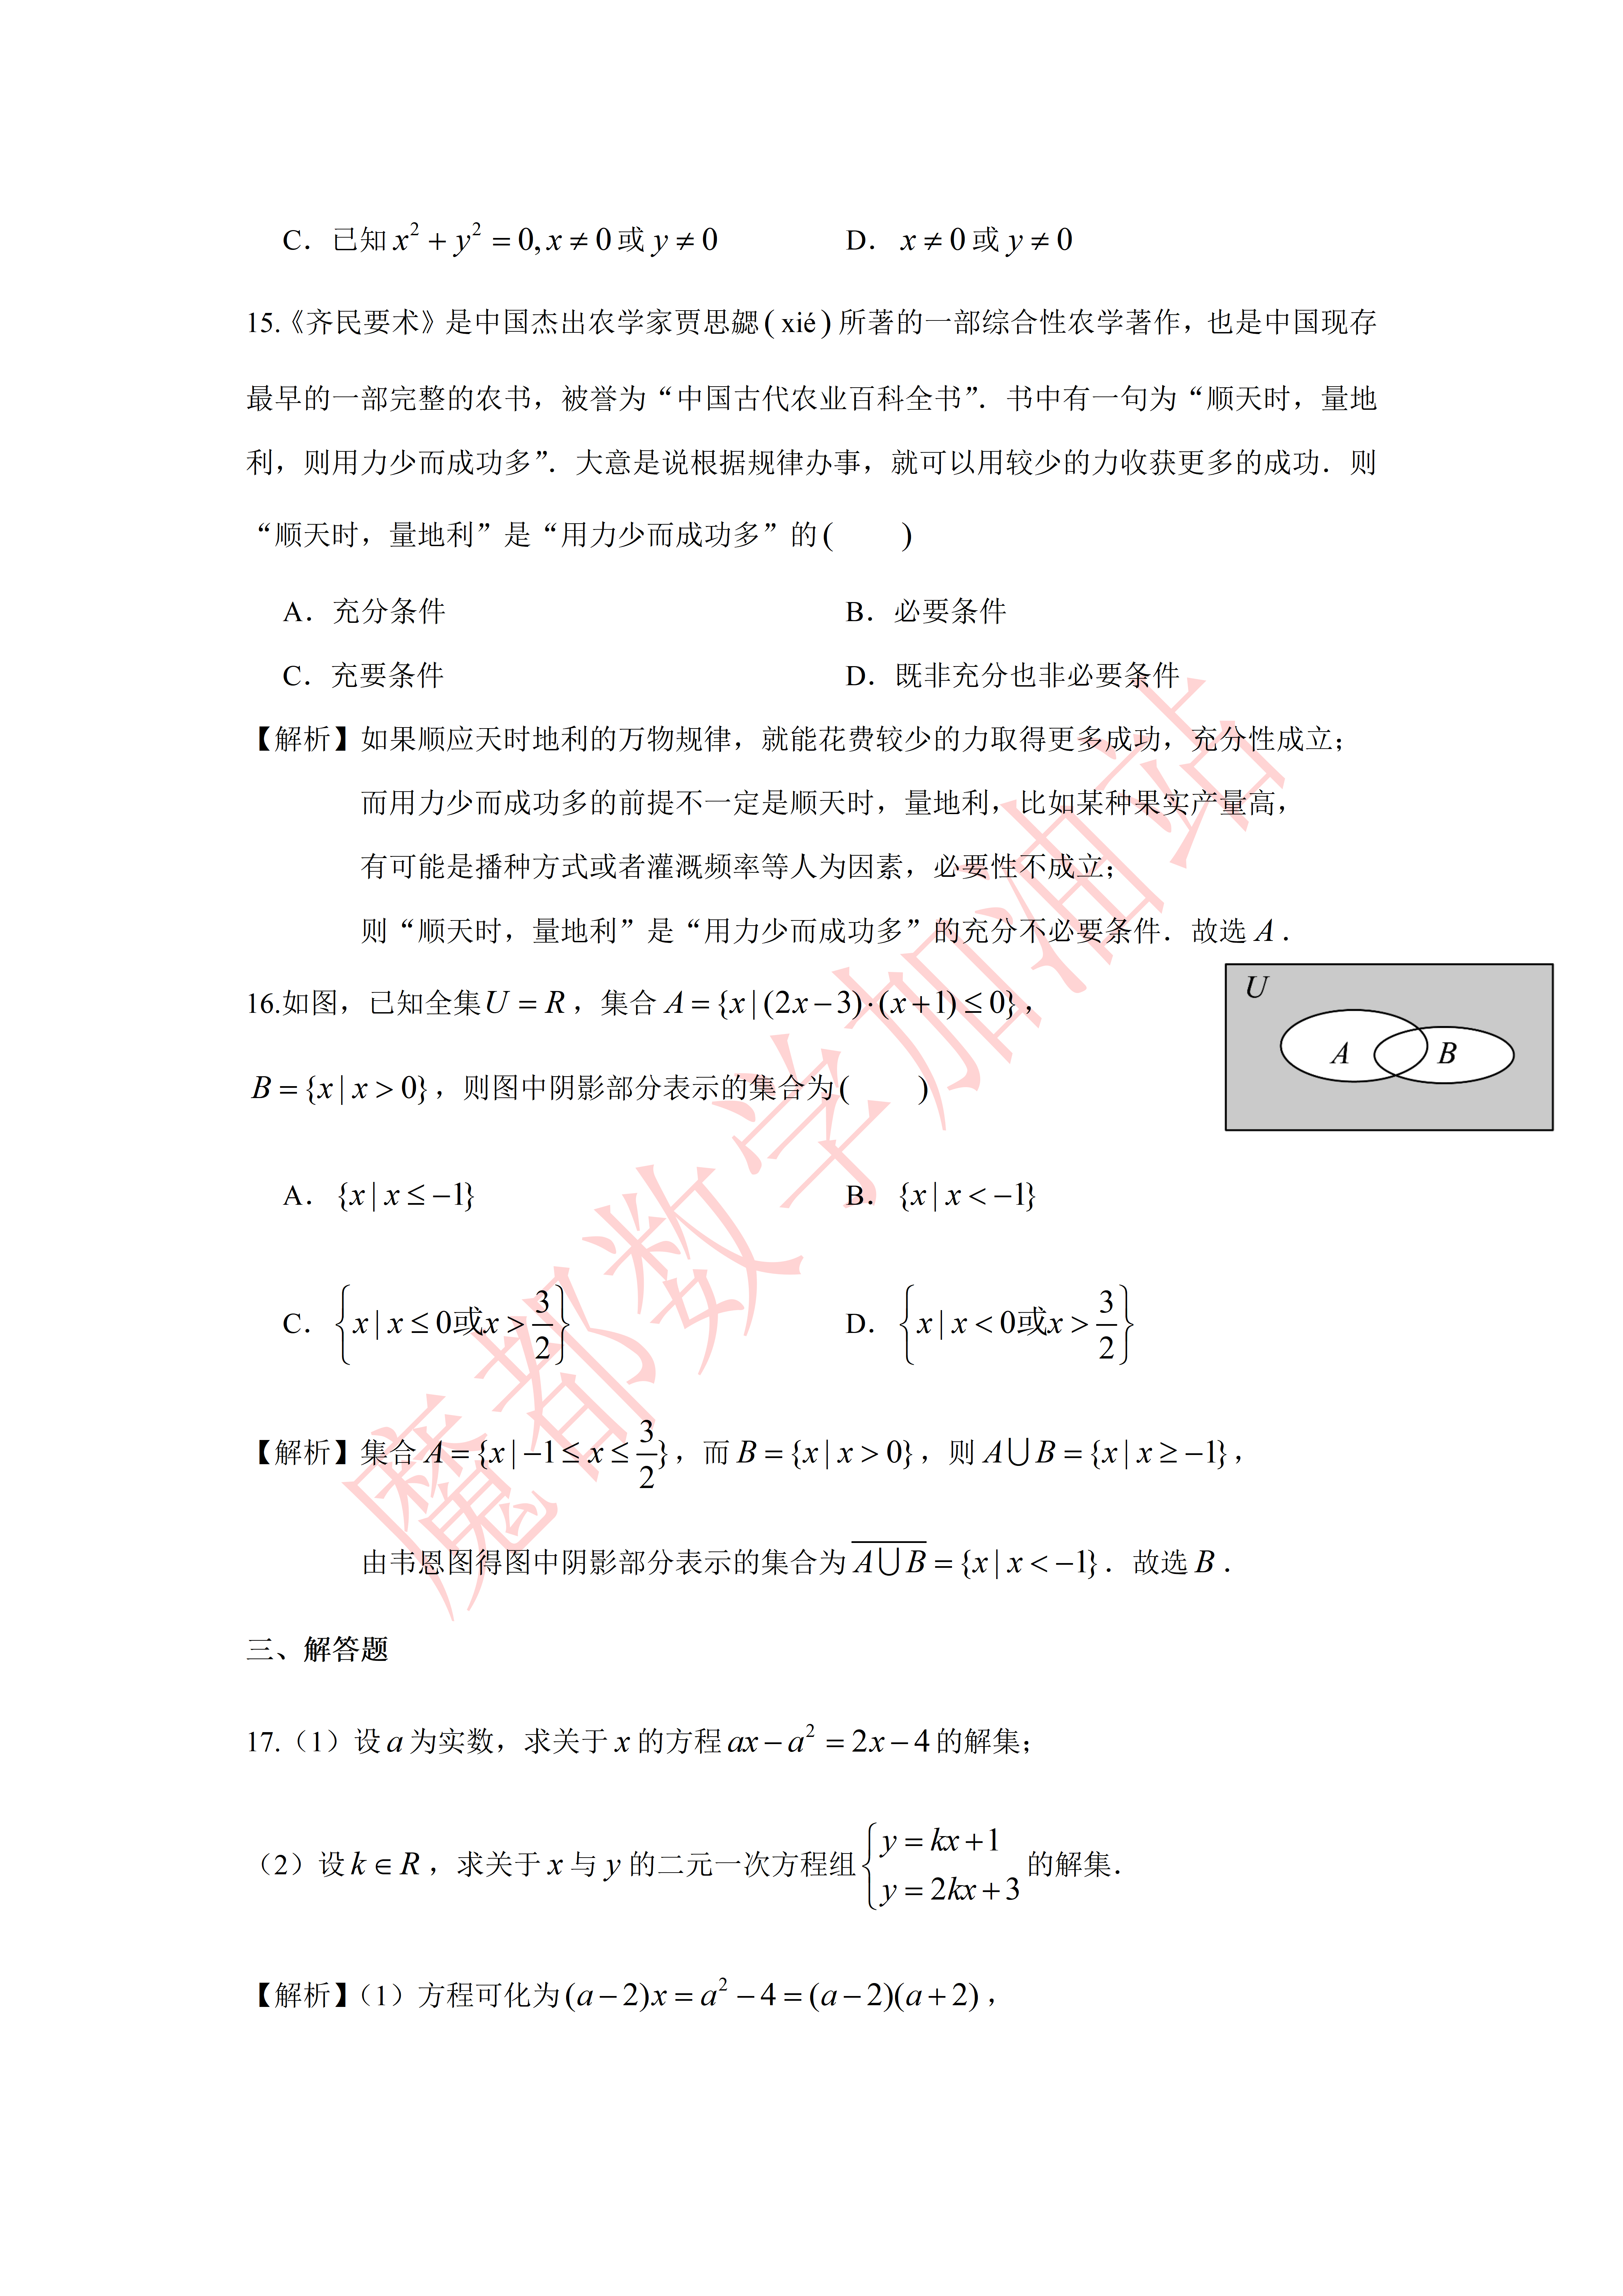
\includegraphics[width=.34\linewidth,trim=3586bp 3410bp 196bp 2818bp,clip]{../原图/高一52_回民中学_9月月考/04.png}
\end{center}

\keepwithprev
A. $\{x\mid x\leqslant-1\}$\qquad B. $\{x\mid x<-1\}$

C. $\left\{x\mid x\leqslant0\text{ 或 }x>\dfrac32\right\}$\qquad D. $\left\{x\mid x<0\text{ 或 }x>\dfrac32\right\}$

\ifanswer
\solbegin
\step{集合 $A=\left\{x\mid-1\leqslant x\leqslant\dfrac32\right\}$，而 $B=\{x\mid x>0\}$，则 $A\cup B=\{x\mid x\geqslant-1\}$，}
\step{由韦恩图得图中阴影部分表示的集合为 $\overline{A\cup B}=\{x\mid x<-1\}$．故选 $B$．}
\solend
\fi

\end{enumerate}

\bigsec{三、解答题}

\begin{enumerate}
\setcounter{enumi}{16}

\item （1）设 $a$ 为实数，求关于 $x$ 的方程 $ax-a^2=2x-4$ 的解集；

（2）设 $k\in\R$，求关于 $x$ 与 $y$ 的二元一次方程组 $\begin{cases}y=kx+1\\y=2kx+3\end{cases}$ 的解集．

\ifanswer
\solbegin
\stepm{(1)}{方程可化为 $(a-2)x=a^2-4=(a-2)(a+2)$，}
\step{当 $a\neq2$ 时，方程的解为 $x=\dfrac{(a-2)(a+2)}{a-2}=a+2$，则解集为 $\{a+2\}$；}
\step{当 $a=2$ 时，方程为 $2x-4=2x-4$，对 $x$ 取一切实数均成立，}
\step{所以解集为 $\R$；}
\stepm{(2)}{$\begin{cases}y=kx+1\\y=2kx+3\end{cases}$，则 $kx+1=2kx+3,kx=-2$，}
\step{当 $k=0$ 时，等式不成立，无解；当 $k\neq0$ 时，$x=-\dfrac2k,y=-1$；}
\step{综上所述，当 $k=0$ 时，解集为 $\varnothing$；当 $k\neq0$ 时，解集为 $\left\{\left(-\dfrac2k,-1\right)\right\}$．}
\solend
\fi

\ansspace[6]

\item 已知命题 $p$：方程 $x^2+6x+m-1=0$ 有两个不等的负根；命题 $q$：方程 $9x^2+6x+m-2=0$ 无实根．

\begin{enumerate}[label=(\arabic*)]
\item 若 $p$ 为真命题，求实数 $m$ 的取值范围；
\item 若 $p,q$ 两命题一真一假，求实数 $m$ 的取值范围．
\end{enumerate}

\ifanswer
\solbegin
\stepm{(1)}{设方程 $x^2+6x+m-1=0$ 两根为 $x_1,x_2$，}
\step{则 $\begin{cases}\Delta>0\\ x_1+x_2<0\\ x_1x_2>0\end{cases}\Rightarrow\begin{cases}36-4(m-1)>0\\ -6<0\\ m-1>0\end{cases}\Rightarrow1<m<10$；}
\stepm{(2)}{若命题 $q$ 为真命题，则 $36-36(m-2)<0\Rightarrow m>3$，}
\step{从而当命题 $q$ 为假命题时，$m\leqslant3$；}
\step{又由（1）得 $p$ 为假命题时，$m\leqslant1$ 或 $m\geqslant10$；}
\step{则当 $p$ 为真命题，$q$ 为假命题时，得 $\begin{cases}1<m<10\\ m\leqslant3\end{cases}\Rightarrow1<m\leqslant3$；}
\step{当 $q$ 为真命题，$p$ 为假命题时，得 $\begin{cases}m\leqslant1\text{ 或 }m\geqslant10\\ m>3\end{cases}\Rightarrow m\geqslant10$；}
\step{综上，当 $p,q$ 两命题一真一假时，$1<m\leqslant3$ 或 $m\geqslant10$.}
\solend
\fi

\ansspace[6]

\item 证明下列两个命题：

\begin{enumerate}[label=(\arabic*)]
\item 设 $ab>0$，求证：$a>b$ 是 $\dfrac1a<\dfrac1b$ 的充要条件．
\item 已知 $a,b$ 为正数，$n$ 为正整数，求证：如果 $a^n>b^n$，那么 $a>b$．
\end{enumerate}

\ifanswer
\solbegin
\stepm{(1)}{先证充分性：因为 $ab>0$ 且 $a>b$，故 $a-b>0$，从而 $\dfrac{a-b}{ab}>0$，}
\step{即 $\dfrac1b-\dfrac1a>0$，即 $\dfrac1a<\dfrac1b$；}
\step{再证必要性：若 $\dfrac1a<\dfrac1b$，则 $\dfrac1a-\dfrac1b=\dfrac{b-a}{ab}<0$，}
\step{又因为 $ab>0$，所以 $b-a<0$，即 $a>b$．}
% 原卷如此，照录未改（第 19 题(1)此句末用全角句号“。”，全卷其余各题末句用“．”，
% 见文件头“原卷笔误/存疑”第 4 条）
\step{综上，$a>b$ 是 $\dfrac1a<\dfrac1b$ 的充要条件。}
\stepm{(2)}{令 $f(x)=x^n,n\in\N^*$，则由幂函数的性质得 $f(x)$ 在第一象限是严格增的，}
\step{而 $a^n>b^n$ 即意味着 $f(a)>f(b)$，且 $a,b$ 为正数，从而 $a>b$．}
\solend
\fi

\ansspace[8]

\item （1）求关于 $x$ 的不等式 $(m-2)x>1-m$ 的解集；

（2）求关于 $x$ 的不等式 $x^2-(a+1)x+a\leqslant0$ 的解集．

\ifanswer
\solbegin
\stepm{(1)}{由不等式 $(m-2)x>1-m$，}
\step{当 $m-2>0$ 时，即 $m>2$ 时，解得 $x>\dfrac{1-m}{m-2}$，}
\step{所以不等式的解集为 $\left(\dfrac{1-m}{m-2},+\infty\right)$；}
\step{当 $m-2=0$ 时，即 $m=2$ 时，不等式即为 $0>-1$ 恒成立，}
\step{即不等式的解集为 $\R$；}
\step{当 $m-2<0$ 时，即 $m<2$ 时，解得 $x<\dfrac{1-m}{m-2}$，}
\step{所以不等式的解集为 $\left(-\infty,\dfrac{1-m}{m-2}\right)$；}
\step{综上，当 $m>2$ 时，解集为 $\left(\dfrac{1-m}{m-2},+\infty\right)$；}
\step{当 $m=2$ 时，解集为 $\R$；}
\step{当 $m<2$ 时，解集为 $\left(-\infty,\dfrac{1-m}{m-2}\right)$．}
\stepm{(2)}{由不等式 $x^2-(a+1)x+a\leqslant0$，可化为 $(x-a)(x-1)\leqslant0$，}
\step{当 $a>1$ 时，解得 $1\leqslant x\leqslant a$，即不等式的解集为 $[1,a]$；}
\step{当 $a=1$ 时，不等式即为 $(x-1)^2\leqslant0$，解得 $x=1$，即不等式的解集为 $\{1\}$；}
\step{当 $a<1$ 时，解得 $a\leqslant x\leqslant1$，即不等式的解集为 $[a,1]$，}
\step{综上，当 $a>1$ 时，解集为 $[1,a]$；}
\step{当 $a=1$ 时，解集为 $\{1\}$；}
\step{当 $a<1$ 时，解集为 $[a,1]$．}
\solend
\fi

\ansspace[10]

\item 已知集合 $A=\{x\mid(x+2)(5-x)\geqslant0\}$，若集合 $B$ 满足 $A\cap B=\varnothing,A\cup B=[-2,7)$．

\begin{enumerate}[label=(\arabic*)]
\item 用区间表示集合 $B$；
\item 若集合 $B$ 是不等式 $-x^2+bx+c>0$ 的解集，求实数 $b,c$ 的值；
\item 已知全集为 $\R$，若关于 $x$ 的不等式 $-1<x-a\leqslant2$ 的解集为 $M$，且“$x\in\overline A$”是“$x\in M$”的必要非充分条件，求实数 $a$ 的取值范围．
\end{enumerate}

\ifanswer
\solbegin
\stepm{(1)}{由题意得 $(x+2)(5-x)\geqslant0\Leftrightarrow(x+2)(x-5)\leqslant0\Rightarrow-2\leqslant x\leqslant5$，}
\step{则 $A=[-2,5]$，又 $A\cap B=\varnothing,A\cup B=[-2,7)$，则 $B=(5,7)$；}
\stepm{(2)}{$-x^2+bx+c>0\Leftrightarrow x^2-bx-c<0$，则 $x^2-bx-c=0$ 两根为 $5,7$，}
\step{则由韦达定理得 $b=12,-c=35\Rightarrow c=-35$；}
\stepm{(3)}{由题意得 $M=(a-1,a+2],\overline A=(-\infty,-2)\cup(5,+\infty)$，}
\step{且“$x\in\overline A$”是“$x\in M$”的必要非充分条件，则 $M$ 是 $\overline A$ 的真子集，}
\step{从而 $a+2<-2$ 或 $a-1\geqslant5$，解得 $a<-4$ 或 $a\geqslant6$，}
\step{所以实数 $a$ 的取值范围为 $(-\infty,-4)\cup[6,+\infty)$．}
\solend
\fi

\ansspace*[10]

\end{enumerate}

\end{document}
"
%
% 原始材料：微信公众号“魔都数学加油站”文章，作者破晓，连载“27学年高一52”；
% 原文标题“27学年高一52——2026-2027年上海市回民中学高一上9月月考”；
% 原文链接：https://mp.weixin.qq.com/s/ndjyozrRQCLl4ba3J8uR7g。
% 该页面用 JS 渲染，未见明确发布日期；页面内时间戳约为 2026-10-06 21:19／21:38，本稿以该时刻记可得日期。
% 正文为 8 张 PNG 页：第 01—07 页 4762×6735，第 08 页 2560×3620（**同一篇各页分辨率不同**），
% 均按页序读取。8 页全为试卷正文页（卷首标题在第 1 页页顶，卷末解答题第 21 题解析止于第 8 页），
% 无封面页、目录页、二维码或宣传页。粉色斜排“魔都数学加油站”为卷面水印，与公众号页脚一并未录入。
%
% 卷首标题：照卷面印作“2026--2027 年回民中学高一上 9 月月考”（公众号标题中的“上海市”
% 卷面标题行没有，本稿照卷面），年份区间按全稿惯例排 en dash。原卷只有一行标题、无副标题。
%
% 篇幅与题号：原卷自第 3 题起编号（第 1、2 题不在本卷内）。填空题 3—12（10 题）、
% 选择题 13—16（4 题）、解答题 17—21（5 题），共 19 题。本稿沿用原节与原题号，
% 只改排为全稿统一的大节样式（原卷小节标题为“一、填空题”“二、选择题”“三、解答题”）。
%
% 讲评版：原卷每题下直接印【答案】或【解析】。**只印【答案】的 1 题**（第 3 题），本稿只给 \ans{}；
% **第 14 题没有任何【答案】/【解析】段**，答案“D”直接印在题干括号内（“应假设(  D  )”），
% 本稿按 高一37 第 13 题的成例把括号留空、答案另提为 \ans{$D$}；
% 其余 17 题都只印【解析】，按全稿口径这类题不另提 \ans{}——其中选择题第 13、15、16 题的结论
% 写在解析末句（“故选 A／A／B”），亦照录在解析内。
%
% 副标题：原卷未印副标题。本稿按“知识模块”口径标作“集合与常用逻辑用语、不等式”：
% 19 题中集合与常用逻辑用语 10 题（集合类 7 题——第 3、4、5、9、12、16、21 题；
% 逻辑类 3 题——第 6、14、15 题），不等式 9 题（含等式性质与一元二次方程：第 7、8、10、11、
% 13、17、18、19、20 题），两类均远超三分之一，故并标。口径同 高一46、高一47、高一48、高一51。
%
% 与原卷的排版差异：
%   ① 原卷每题下直接印【答案】/【解析】，本稿按全稿惯例将答案与解析置于答案版，试卷版保持干净；
%      第 14 题印在题干括号内的答案“D”同样移入 \ans{}，见上；
%   ② 原卷未印副标题，本稿按“知识模块”口径补出；
%   ③ 原卷填空横线约两个字宽，本稿按全稿惯例统一排 \blankline[4.4em]；
%      选择题的作答括号原卷排半角“(    )”，本稿按全稿惯例排 \mbox{（\quad）}；
%   ④ 原卷实数集、自然数集排斜体/粗体 $R$、$\mathbf{R}$、$N$，本稿按全稿惯例改用 $\R$、$\N$；
%      空集记号统一为 \varnothing；
%   ⑤ 第 8 题题干与解析两处“两个实数分别为 $x_1$、$x_2$”原卷即用顿号，第 10、13 题等处
%      原卷在数学式内用半角逗号（如 $x_1,x_2$、$a,b,c\in R$），两份均照录未强改；
%      句末句点按全稿惯例排西文句点，句中句点（第 9、12、15、21 题）照原卷排全角“．”；
%   ⑥ 第 17、20 题原卷把子问标号“（1）”排在该题题号同一行，本稿照原卷仍排同一行（同 高一34 的
%      做法）；第 18、19、21 题的子问原卷各自另起一行，本稿按全稿惯例用 enumerate 的 (1)(2)(3)；
%      解析中的子问标号一律用 \stepm{(1)}{…}；
%   ⑦ 第 16 题的韦恩图原卷排在题干与选项右侧的浮动位置，本稿居中排在题干之后、选项之前，
%      并加 \needvspace 整块推走（守卫写在 \item 之前）；图自原图第 4 页裁切（trim），不另存图片文件；
%   ⑧ 每道解答题原卷未留作答空白，本稿按全稿惯例加 \ansspace。
%
% 原卷笔误/存疑（均照录未改，正文对应处另有 % 注）：
%   1. 第 8 题题干与解析首行两处均作“两个实数分别为 $x_1$、$x_2$”，按文意应为“两个实数**根**”
%      （疑脱“根”字，第 10 题同位置作“两个实根分别是”）；
%   2. 第 4 题解析“满足条件的 $A$ 的个数为集合 $\{0,1,3\}$ 的真子集，即 7 个”，
%      “个数为……真子集”表述不严（应为“……的真子集的个数”）；$\{0,1,3\}$ 的真子集 7 个，结论无误；
%   3. 第 6 题解析第 2 行“当 $a=10,b=0.2$ 时，$a+b>2$，且 $ab>1$，所以 $a>1$，且 $b>1$ 不成立”
%      ——此处是举反例，“所以”按文意应为“但”（$a=10,b=0.2$ 与“$a>1$ 且 $b>1$”不成立之间是转折，
%      非因果）；
%   4. 第 19 题 (1) 解析末行“综上，$a>b$ 是 $\dfrac1a<\dfrac1b$ 的充要条件。”用全角句号“。”，
%      全卷其余各题末句均用“．”，体例不一，照录；
%   5. 第 20 题第 (1) 问解析先按 $m>2$、$m=2$、$m<2$ 三种情况各给出解集，末三行又“综上”重述一遍，
%      与原卷一致（内容重复，非笔误）；
%   6. 第 18 题题干第 (2) 问“若 $p,q$ 两命题一真一假”，正文照录原卷所用半角逗号（未改顿号）。
%
% 插图：1 张，自原图裁切（无 \begin{tikzpicture} 重排）：
%   · 第 16 题题干韦恩图（全集 $U$ 矩形内两相交椭圆 $A$、$B$，灰色为阴影部分）
%     ——原图第 04 页，原卷排于题干与选项右侧。
%     裁框：x 3594–4558、y 2826–3317（即矩形外框，四周各留 4px），
%     trim=3590bp 3414bp 200bp 2822bp（左／下／右／上），页宽 4762、页高 6735。
%
\documentclass[a4paper,11pt]{article}
\usepackage{common}

\begin{document}

\examtitlest[3]{2026--2027 年回民中学高一上 9 月月考}{集合与常用逻辑用语、不等式}

\bigsec{一、填空题}

\begin{enumerate}
\setcounter{enumi}{2}

\item 用列举法写出下列集合 $\{(x,y)\mid x+y=2,x\in\N,y\in\N\}=$\blankline[4.4em].

\ifanswer
\ans{$\{(0,2),(1,1),(2,0)\}$}
\fi

\item 设集合 $A$ 满足 $\{-1,2\}\sub A\subset\{-1,0,1,2,3\}$，则满足条件的 $A$ 有\blankline[4.4em]个.

\ifanswer
\solbegin
\step{满足条件的 $A$ 的个数为集合 $\{0,1,3\}$ 的真子集，即 $7$ 个.}
\solend
\fi

\item 已知集合 $A=\{2,(a+1)^2,a^2+2\}$，且 $1\in A$，则实数 $a$ 的值为\blankline[4.4em].

\ifanswer
\solbegin
\step{因为 $1\in A$，而 $a^2+2\geqslant2$，所以 $(a+1)^2=1$，解得 $a=0$ 或 $a=-2$，}
\step{$a=0$ 时，$a^2+2=2$，不合题意，$a=-2$ 时，$a^2+2=6$，满足题意，}
\step{所以 $a=-2$.}
\solend
\fi

\item 已知 $a,b$ 是实数，则“$a>1$，且 $b>1$”是“$a+b>2$，且 $ab>1$”的\blankline[4.4em]条件.

\ifanswer
\solbegin
\step{$a,b$ 是实数，则“$a>1$，且 $b>1$”$\Rightarrow$“$a+b>2$，且 $ab>1$”正确，}
% 原卷如此，照录未改（第 6 题解析此处作“所以 $a>1$，且 $b>1$ 不成立”，按文意为转折，
% 见文件头“原卷笔误/存疑”第 3 条）
\step{当 $a=10,b=0.2$ 时，$a+b>2$，且 $ab>1$，所以 $a>1$，且 $b>1$ 不成立，}
\step{即前者是推出后者，后者推不出前者，}
\step{所以“$a>1$，且 $b>1$”是“$a+b>2$，且 $ab>1$”的充分而不必要条件.}
\solend
\fi

\item 已知等式 $2x^2-3x-1=a(x-1)^2+b(x-1)+c$ 恒成立，其中 $a,b,c$ 为常数，则 $a+b-c=$\blankline[4.4em].

\ifanswer
\solbegin
\step{将等式右侧展开整理得 $a(x-1)^2+b(x-1)+c=ax^2+(-2a+b)x+(a-b+c)$，}
\step{左右两边多项式恒等，对应次数的系数必须相等：}
\step{则 $a=2,-2a+b=-3$，代入 $a=2$ 得 $b=1$，$a-b+c=-1$，}
\step{代入 $a=2,b=1$ 得 $c=-2$，得 $a+b-c=2+1-(-2)=5$.}
\solend
\fi

% 原卷如此，照录未改（第 8 题题干与解析首行两处“两个实数分别为”疑脱“根”字，
% 见文件头“原卷笔误/存疑”第 1 条）
\item 若关于 $x$ 的二次方程 $x^2+mx+4m^2-3=0$ 的两个实数分别为 $x_1$、$x_2$，且满足 $x_1+x_2=x_1x_2$，则实数 $m$ 的值为\blankline[4.4em].

\ifanswer
\solbegin
% 原卷如此，照录未改（此处“两个实数分别为”同题干，疑脱“根”字）
\step{二次方程 $x^2+mx+4m^2-3=0$ 的两个实数分别为 $x_1$、$x_2$，}
\step{则有 $\Delta=m^2-4(4m^2-3)\geqslant0$，变形得 $m^2\leqslant\dfrac45$，}
\step{则 $x_1+x_2=-m$，$x_1x_2=(4m^2-3)$，}
\step{若 $x_1+x_2=x_1x_2$，则有 $-m=4m^2-3$，解得 $m=-1$ 或 $\dfrac34$，}
\step{又 $m^2\leqslant\dfrac45$，则 $m=\dfrac34$.}
\solend
\fi

\item 设集合 $A=\{x\mid x^2=1\}$，$B=\{x\mid ax=1\}$．若 $A\cap B=B$，则实数 $a$ 的值为\blankline[4.4em].

\ifanswer
\solbegin
\step{集合 $A=\{x\mid x^2=1\}=\{-1,1\}$，$B=\{x\mid ax=1\}$，$A\cap B=B$，所以 $B\sub A$，}
\step{当 $a=0$ 时，$B=\varnothing$，成立；}
\step{当 $a\neq0$ 时，$B=\left\{\dfrac1a\right\}$，则 $\dfrac1a=-1$ 或 $\dfrac1a=1$，解得 $a=-1$ 或 $a=1$，}
\step{所以实数 $a$ 的值为 $0$ 或 $1$ 或 $-1$.}
\solend
\fi

\item 已知关于 $x$ 的一元二次方程 $x^2+3x-3=0$ 的两个实根分别是 $x_1,x_2$，则以 $-\dfrac1{x_1},-\dfrac1{x_2}$ 为根且二次项系数是 $1$ 的一元二次方程为\blankline[4.4em].

\ifanswer
\solbegin
\step{因为 $x_1,x_2$ 是一元二次方程 $x^2+3x-3=0$ 的两个实根，}
\step{所以 $x_1+x_2=-3,x_1x_2=-3$，}
\step{所以 $-\dfrac1{x_1}+\left(-\dfrac1{x_2}\right)=-\dfrac{x_1+x_2}{x_1x_2}=-1$，$-\dfrac1{x_1}\cdot\left(-\dfrac1{x_2}\right)=\dfrac1{x_1x_2}=-\dfrac13$，}
\step{所以一元二次方程为 $x^2+x-\dfrac13=0$.}
\solend
\fi

\item 若关于 $x$ 的不等式 $(a-2)x^2+2(a-2)x-4<0$ 的解集是 $\R$，则实数 $a$ 的取值范围是\blankline[4.4em].

\ifanswer
\solbegin
\step{当 $a=2$ 时，不等式化为 $-4<0$ 对于任意实数 $x$ 都成立，因此 $a=2$ 满足题意；}
\step{当 $a\neq2$ 时，要使关于 $x$ 的不等式 $(a-2)x^2+2(a-2)x-4<0$ 的解集为 $\R$，}
\step{则 $\begin{cases}a-2<0\\ \Delta=4(a-2)^2+16(a-2)<0\end{cases}$，解得 $-2<a<2$．}
\step{综上，$a$ 的取值范围为 $(-2,2]$．}
\solend
\fi

\item 设非空集合 $A$、$B$，定义 $A\times B=\{x\mid x\in(A\cup B),x\notin(A\cap B)\}$．已知 $A=\{x\mid0\leqslant x\leqslant2\}$，$B=\{y\mid y\geqslant0\}$，则 $A\times B=$\blankline[4.4em].

\ifanswer
\solbegin
\step{由于 $A=\{x\mid0\leqslant x\leqslant2\}$，$B=\{y\mid y\geqslant0\}=\{x\mid x\geqslant0\}$，}
\step{所以 $A\cup B=\{x\mid x\geqslant0\}$，$A\cap B=\{x\mid0\leqslant x\leqslant2\}$，故 $A\times B=\{x\mid x>2\}$．}
\solend
\fi

\end{enumerate}

\bigsec{二、选择题}

\begin{enumerate}
\setcounter{enumi}{12}

\item 已知 $a,b,c\in\R$ 且 $a>b$，则下列不等式一定成立的是\mbox{（\quad）}

\keepwithprev
A. $\dfrac{a}{c^2+1}>\dfrac{b}{c^2+1}$\qquad B. $\dfrac1a<\dfrac1b$

C. $ac>bc$\qquad D. $a^2>b^2$

\ifanswer
\solbegin
\step{对于 A：因为 $c^2+1>0$ 恒成立，且 $a>b$，所以 $\dfrac{a}{c^2+1}>\dfrac{b}{c^2+1}$ 一定成立，}
\step{所以 A 正确；}
\step{对于 B：当 $a=1,b=-1$ 时，满足 $a>b$，此时 $\dfrac1a=1>\dfrac1b=-1$，所以 B 错误；}
\step{对于 C：当 $c<0$ 时，由 $a>b$，得 $ac<bc$，所以 C 错误；}
\step{对于 D：当 $a=1,b=-2$ 时，满足 $a>b$，此时 $a^2=1<b^2=4$，所以 D 错误；}
\step{故选 $A$．}
\solend
\fi

% 注：本题的答案“D”原卷直接印在题干末尾的括号内（“应假设(  D  )”），且没有单独的
%     【答案】/【解析】段，本稿按 高一37 第 13 题的成例把括号留空、另提为 \ans{}，
%     见文件头“与原卷的排版差异”①。
\item 用反证法证明：“已知 $x,y\in\R$,$x^2+y^2=0$，求证：$x=y=0$”时，应假设\mbox{（\quad）}

\keepwithprev
A. 已知 $x^2+y^2=0,x\neq0$ 且 $y\neq0$\qquad B. $x\neq0$ 且 $y\neq0$

C. 已知 $x^2+y^2=0,x\neq0$ 或 $y\neq0$\qquad D. $x\neq0$ 或 $y\neq0$

\ans{$D$}

\item 《齐民要术》是中国杰出农学家贾思勰（xié）所著的一部综合性农学著作，也是中国现存最早的一部完整的农书，被誉为“中国古代农业百科全书”．书中有一句为“顺天时，量地利，则用力少而成功多”．大意是说根据规律办事，就可以用较少的力收获更多的成功．则“顺天时，量地利”是“用力少而成功多”的\mbox{（\quad）}

\keepwithprev
A. 充分条件\qquad B. 必要条件

C. 充要条件\qquad D. 既非充分也非必要条件

\ifanswer
\solbegin
\step{如果顺应天时地利的万物规律，就能花费较少的力取得更多成功，充分性成立；}
\step{而用力少而成功多的前提不一定是顺天时，量地利，比如某种果实产量高，}
\step{有可能是播种方式或者灌溉频率等人为因素，必要性不成立；}
\step{则“顺天时，量地利”是“用力少而成功多”的充分不必要条件．故选 $A$．}
\solend
\fi

\needvspace{13\baselineskip}

\item 如图，已知全集 $U=\R$，集合 $A=\{x\mid(2x-3)\cdot(x+1)\leqslant0\}$，$B=\{x\mid x>0\}$，则图中阴影部分表示的集合为\mbox{（\quad）}

\begin{center}
% 原图第 4 页题干韦恩图直接裁取（原卷排于题干与选项右侧）。
% 裁框取矩形外框 x 3590–4558、y 2822–3321，再向外各留 4px（即 x 3586–4562、y 2818–3325），
% trim=左 3586bp／下 3410bp／右 196bp／上 2818bp（页宽 4762、页高 6735）。
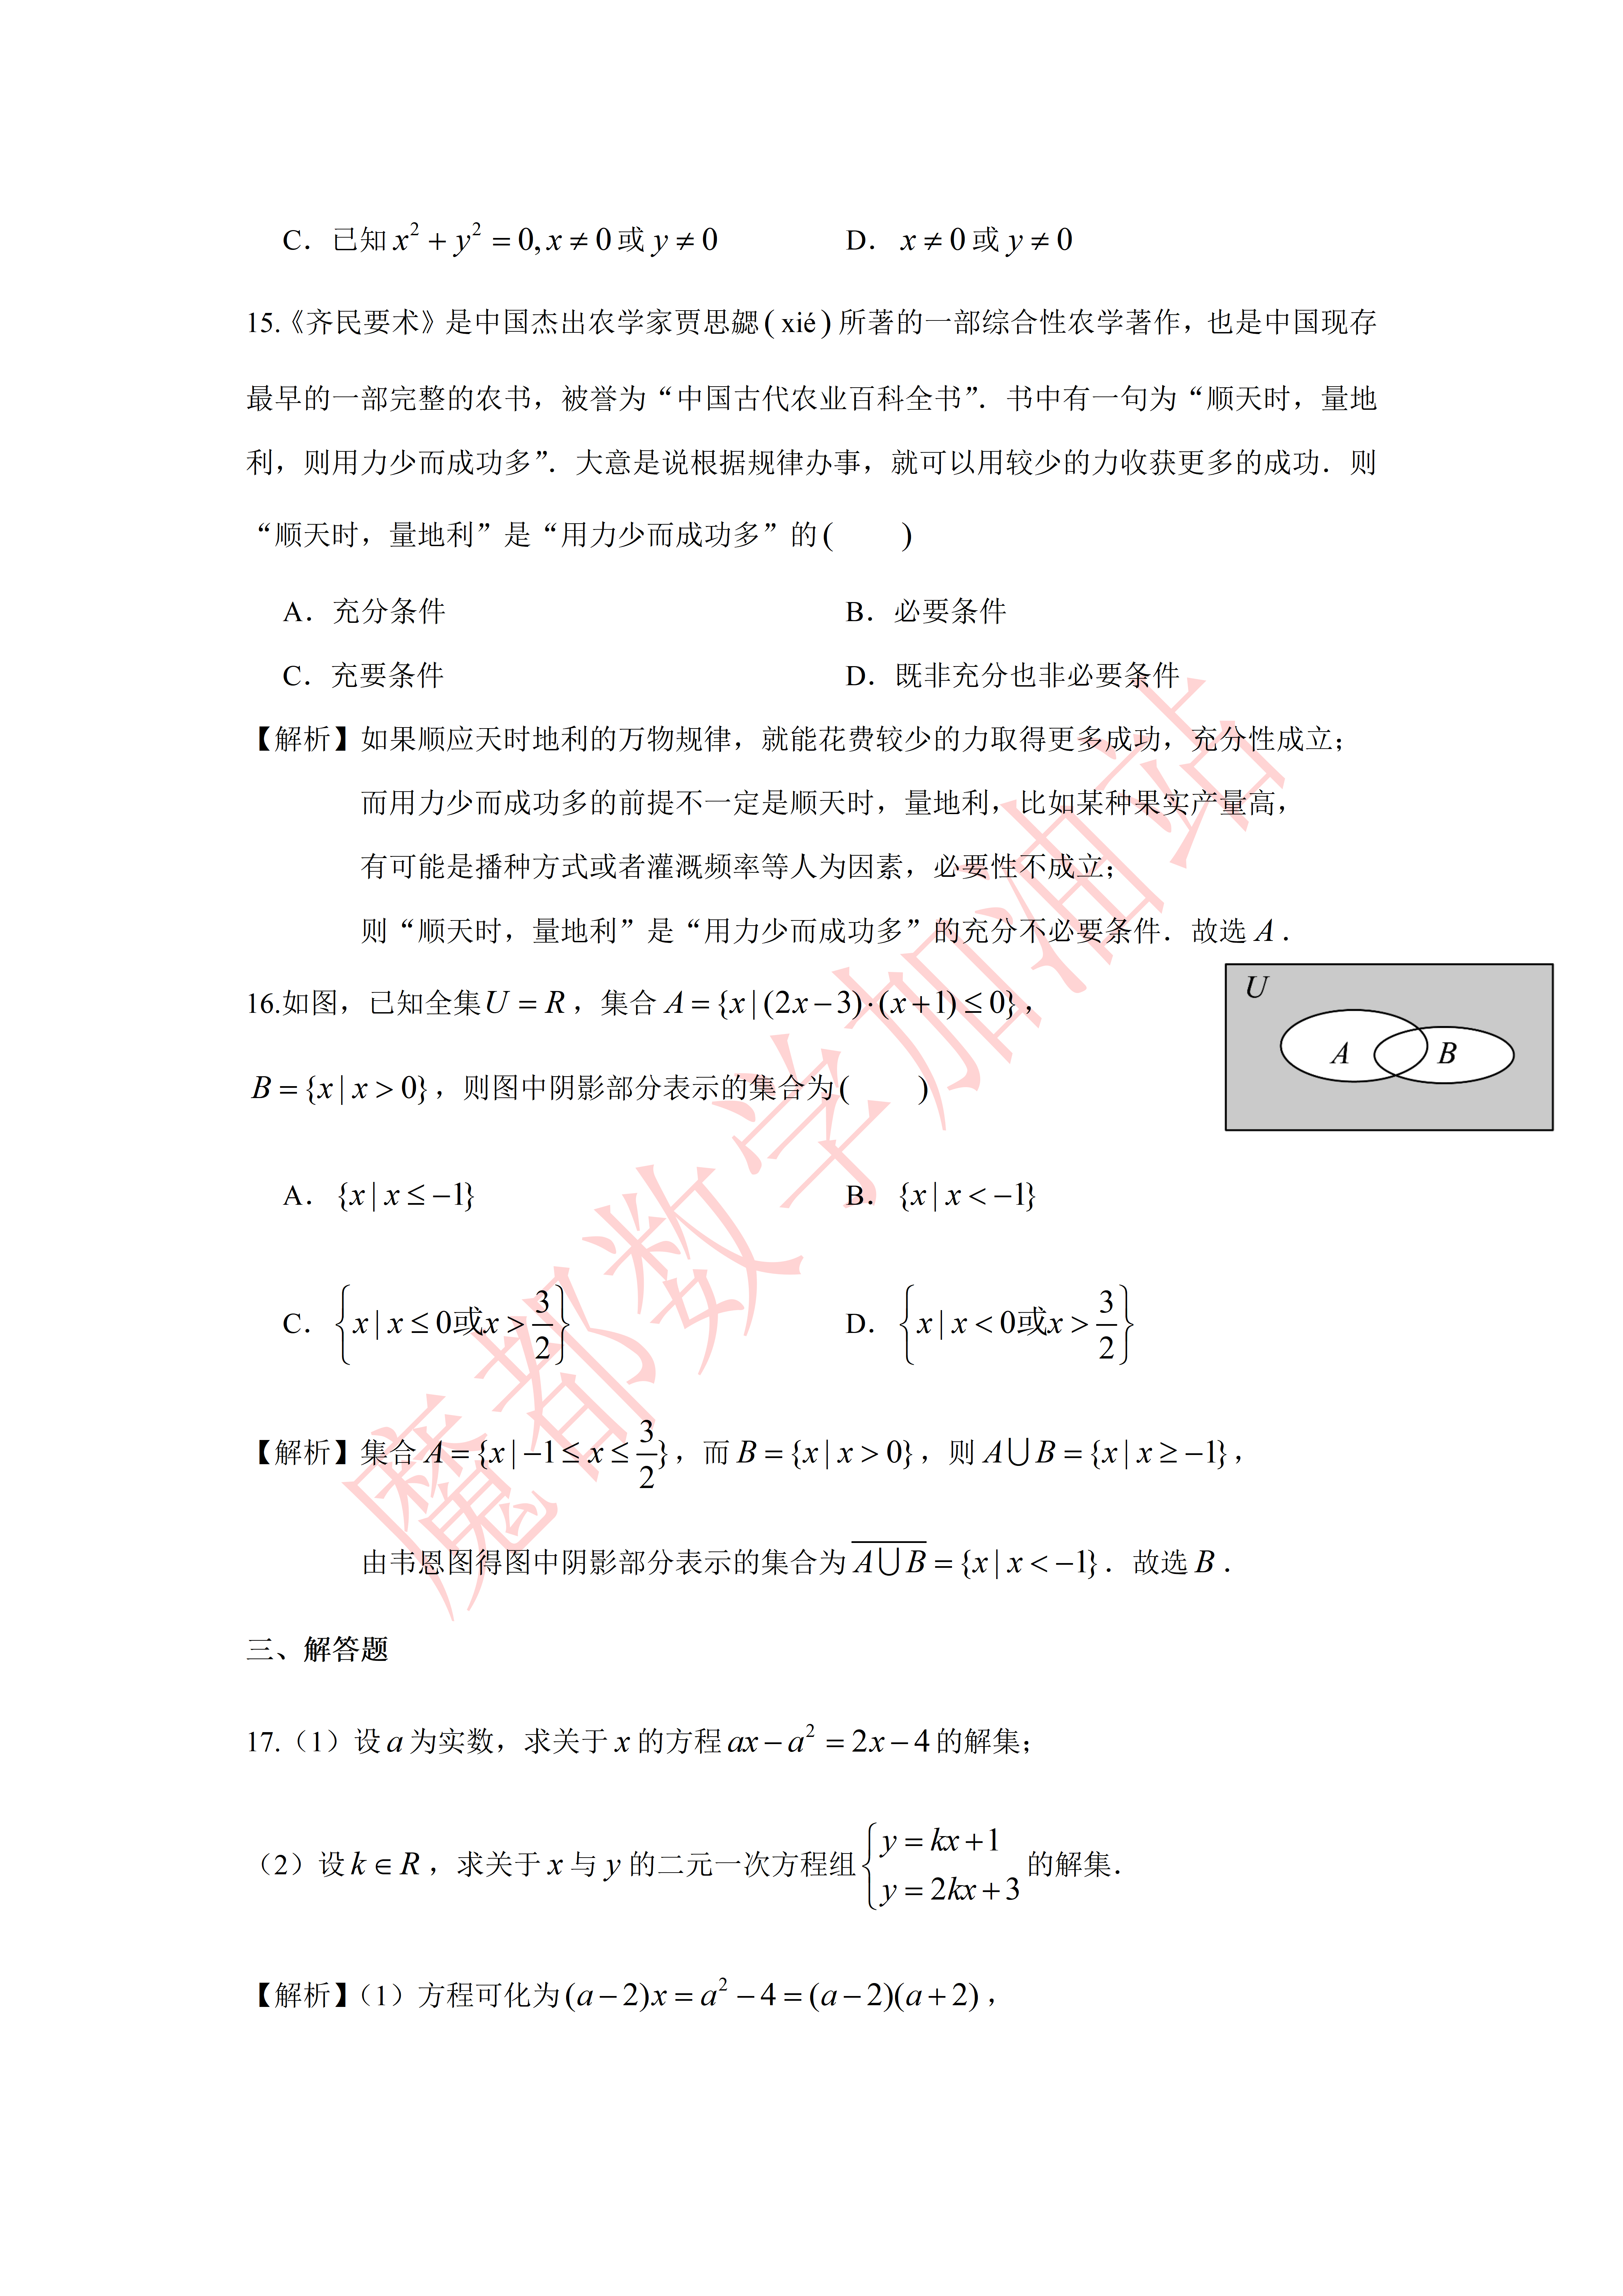
\includegraphics[width=.34\linewidth,trim=3586bp 3410bp 196bp 2818bp,clip]{../原图/高一52_回民中学_9月月考/04.png}
\end{center}

\keepwithprev
A. $\{x\mid x\leqslant-1\}$\qquad B. $\{x\mid x<-1\}$

C. $\left\{x\mid x\leqslant0\text{ 或 }x>\dfrac32\right\}$\qquad D. $\left\{x\mid x<0\text{ 或 }x>\dfrac32\right\}$

\ifanswer
\solbegin
\step{集合 $A=\left\{x\mid-1\leqslant x\leqslant\dfrac32\right\}$，而 $B=\{x\mid x>0\}$，则 $A\cup B=\{x\mid x\geqslant-1\}$，}
\step{由韦恩图得图中阴影部分表示的集合为 $\overline{A\cup B}=\{x\mid x<-1\}$．故选 $B$．}
\solend
\fi

\end{enumerate}

\bigsec{三、解答题}

\begin{enumerate}
\setcounter{enumi}{16}

\item （1）设 $a$ 为实数，求关于 $x$ 的方程 $ax-a^2=2x-4$ 的解集；

（2）设 $k\in\R$，求关于 $x$ 与 $y$ 的二元一次方程组 $\begin{cases}y=kx+1\\y=2kx+3\end{cases}$ 的解集．

\ifanswer
\solbegin
\stepm{(1)}{方程可化为 $(a-2)x=a^2-4=(a-2)(a+2)$，}
\step{当 $a\neq2$ 时，方程的解为 $x=\dfrac{(a-2)(a+2)}{a-2}=a+2$，则解集为 $\{a+2\}$；}
\step{当 $a=2$ 时，方程为 $2x-4=2x-4$，对 $x$ 取一切实数均成立，}
\step{所以解集为 $\R$；}
\stepm{(2)}{$\begin{cases}y=kx+1\\y=2kx+3\end{cases}$，则 $kx+1=2kx+3,kx=-2$，}
\step{当 $k=0$ 时，等式不成立，无解；当 $k\neq0$ 时，$x=-\dfrac2k,y=-1$；}
\step{综上所述，当 $k=0$ 时，解集为 $\varnothing$；当 $k\neq0$ 时，解集为 $\left\{\left(-\dfrac2k,-1\right)\right\}$．}
\solend
\fi

\ansspace[6]

\item 已知命题 $p$：方程 $x^2+6x+m-1=0$ 有两个不等的负根；命题 $q$：方程 $9x^2+6x+m-2=0$ 无实根．

\begin{enumerate}[label=(\arabic*)]
\item 若 $p$ 为真命题，求实数 $m$ 的取值范围；
\item 若 $p,q$ 两命题一真一假，求实数 $m$ 的取值范围．
\end{enumerate}

\ifanswer
\solbegin
\stepm{(1)}{设方程 $x^2+6x+m-1=0$ 两根为 $x_1,x_2$，}
\step{则 $\begin{cases}\Delta>0\\ x_1+x_2<0\\ x_1x_2>0\end{cases}\Rightarrow\begin{cases}36-4(m-1)>0\\ -6<0\\ m-1>0\end{cases}\Rightarrow1<m<10$；}
\stepm{(2)}{若命题 $q$ 为真命题，则 $36-36(m-2)<0\Rightarrow m>3$，}
\step{从而当命题 $q$ 为假命题时，$m\leqslant3$；}
\step{又由（1）得 $p$ 为假命题时，$m\leqslant1$ 或 $m\geqslant10$；}
\step{则当 $p$ 为真命题，$q$ 为假命题时，得 $\begin{cases}1<m<10\\ m\leqslant3\end{cases}\Rightarrow1<m\leqslant3$；}
\step{当 $q$ 为真命题，$p$ 为假命题时，得 $\begin{cases}m\leqslant1\text{ 或 }m\geqslant10\\ m>3\end{cases}\Rightarrow m\geqslant10$；}
\step{综上，当 $p,q$ 两命题一真一假时，$1<m\leqslant3$ 或 $m\geqslant10$.}
\solend
\fi

\ansspace[6]

\item 证明下列两个命题：

\begin{enumerate}[label=(\arabic*)]
\item 设 $ab>0$，求证：$a>b$ 是 $\dfrac1a<\dfrac1b$ 的充要条件．
\item 已知 $a,b$ 为正数，$n$ 为正整数，求证：如果 $a^n>b^n$，那么 $a>b$．
\end{enumerate}

\ifanswer
\solbegin
\stepm{(1)}{先证充分性：因为 $ab>0$ 且 $a>b$，故 $a-b>0$，从而 $\dfrac{a-b}{ab}>0$，}
\step{即 $\dfrac1b-\dfrac1a>0$，即 $\dfrac1a<\dfrac1b$；}
\step{再证必要性：若 $\dfrac1a<\dfrac1b$，则 $\dfrac1a-\dfrac1b=\dfrac{b-a}{ab}<0$，}
\step{又因为 $ab>0$，所以 $b-a<0$，即 $a>b$．}
% 原卷如此，照录未改（第 19 题(1)此句末用全角句号“。”，全卷其余各题末句用“．”，
% 见文件头“原卷笔误/存疑”第 4 条）
\step{综上，$a>b$ 是 $\dfrac1a<\dfrac1b$ 的充要条件。}
\stepm{(2)}{令 $f(x)=x^n,n\in\N^*$，则由幂函数的性质得 $f(x)$ 在第一象限是严格增的，}
\step{而 $a^n>b^n$ 即意味着 $f(a)>f(b)$，且 $a,b$ 为正数，从而 $a>b$．}
\solend
\fi

\ansspace[8]

\item （1）求关于 $x$ 的不等式 $(m-2)x>1-m$ 的解集；

（2）求关于 $x$ 的不等式 $x^2-(a+1)x+a\leqslant0$ 的解集．

\ifanswer
\solbegin
\stepm{(1)}{由不等式 $(m-2)x>1-m$，}
\step{当 $m-2>0$ 时，即 $m>2$ 时，解得 $x>\dfrac{1-m}{m-2}$，}
\step{所以不等式的解集为 $\left(\dfrac{1-m}{m-2},+\infty\right)$；}
\step{当 $m-2=0$ 时，即 $m=2$ 时，不等式即为 $0>-1$ 恒成立，}
\step{即不等式的解集为 $\R$；}
\step{当 $m-2<0$ 时，即 $m<2$ 时，解得 $x<\dfrac{1-m}{m-2}$，}
\step{所以不等式的解集为 $\left(-\infty,\dfrac{1-m}{m-2}\right)$；}
\step{综上，当 $m>2$ 时，解集为 $\left(\dfrac{1-m}{m-2},+\infty\right)$；}
\step{当 $m=2$ 时，解集为 $\R$；}
\step{当 $m<2$ 时，解集为 $\left(-\infty,\dfrac{1-m}{m-2}\right)$．}
\stepm{(2)}{由不等式 $x^2-(a+1)x+a\leqslant0$，可化为 $(x-a)(x-1)\leqslant0$，}
\step{当 $a>1$ 时，解得 $1\leqslant x\leqslant a$，即不等式的解集为 $[1,a]$；}
\step{当 $a=1$ 时，不等式即为 $(x-1)^2\leqslant0$，解得 $x=1$，即不等式的解集为 $\{1\}$；}
\step{当 $a<1$ 时，解得 $a\leqslant x\leqslant1$，即不等式的解集为 $[a,1]$，}
\step{综上，当 $a>1$ 时，解集为 $[1,a]$；}
\step{当 $a=1$ 时，解集为 $\{1\}$；}
\step{当 $a<1$ 时，解集为 $[a,1]$．}
\solend
\fi

\ansspace[10]

\item 已知集合 $A=\{x\mid(x+2)(5-x)\geqslant0\}$，若集合 $B$ 满足 $A\cap B=\varnothing,A\cup B=[-2,7)$．

\begin{enumerate}[label=(\arabic*)]
\item 用区间表示集合 $B$；
\item 若集合 $B$ 是不等式 $-x^2+bx+c>0$ 的解集，求实数 $b,c$ 的值；
\item 已知全集为 $\R$，若关于 $x$ 的不等式 $-1<x-a\leqslant2$ 的解集为 $M$，且“$x\in\overline A$”是“$x\in M$”的必要非充分条件，求实数 $a$ 的取值范围．
\end{enumerate}

\ifanswer
\solbegin
\stepm{(1)}{由题意得 $(x+2)(5-x)\geqslant0\Leftrightarrow(x+2)(x-5)\leqslant0\Rightarrow-2\leqslant x\leqslant5$，}
\step{则 $A=[-2,5]$，又 $A\cap B=\varnothing,A\cup B=[-2,7)$，则 $B=(5,7)$；}
\stepm{(2)}{$-x^2+bx+c>0\Leftrightarrow x^2-bx-c<0$，则 $x^2-bx-c=0$ 两根为 $5,7$，}
\step{则由韦达定理得 $b=12,-c=35\Rightarrow c=-35$；}
\stepm{(3)}{由题意得 $M=(a-1,a+2],\overline A=(-\infty,-2)\cup(5,+\infty)$，}
\step{且“$x\in\overline A$”是“$x\in M$”的必要非充分条件，则 $M$ 是 $\overline A$ 的真子集，}
\step{从而 $a+2<-2$ 或 $a-1\geqslant5$，解得 $a<-4$ 或 $a\geqslant6$，}
\step{所以实数 $a$ 的取值范围为 $(-\infty,-4)\cup[6,+\infty)$．}
\solend
\fi

\ansspace*[10]

\end{enumerate}

\end{document}
"
% 紧凑版：xelatex "\def\iscompact{1}% 高一52_回民中学_9月月考.tex
%   —— 高一上数学“2026-2027 年回民中学高一上 9 月月考”（讲评版）
% 试卷版：xelatex 高一52_回民中学_9月月考.tex
% 答案版：xelatex "\def\isanswer{1}% 高一52_回民中学_9月月考.tex
%   —— 高一上数学“2026-2027 年回民中学高一上 9 月月考”（讲评版）
% 试卷版：xelatex 高一52_回民中学_9月月考.tex
% 答案版：xelatex "\def\isanswer{1}% 高一52_回民中学_9月月考.tex
%   —— 高一上数学“2026-2027 年回民中学高一上 9 月月考”（讲评版）
% 试卷版：xelatex 高一52_回民中学_9月月考.tex
% 答案版：xelatex "\def\isanswer{1}\input{高一52_回民中学_9月月考.tex}"
% 紧凑版：xelatex "\def\iscompact{1}\input{高一52_回民中学_9月月考.tex}"
%
% 原始材料：微信公众号“魔都数学加油站”文章，作者破晓，连载“27学年高一52”；
% 原文标题“27学年高一52——2026-2027年上海市回民中学高一上9月月考”；
% 原文链接：https://mp.weixin.qq.com/s/ndjyozrRQCLl4ba3J8uR7g。
% 该页面用 JS 渲染，未见明确发布日期；页面内时间戳约为 2026-10-06 21:19／21:38，本稿以该时刻记可得日期。
% 正文为 8 张 PNG 页：第 01—07 页 4762×6735，第 08 页 2560×3620（**同一篇各页分辨率不同**），
% 均按页序读取。8 页全为试卷正文页（卷首标题在第 1 页页顶，卷末解答题第 21 题解析止于第 8 页），
% 无封面页、目录页、二维码或宣传页。粉色斜排“魔都数学加油站”为卷面水印，与公众号页脚一并未录入。
%
% 卷首标题：照卷面印作“2026--2027 年回民中学高一上 9 月月考”（公众号标题中的“上海市”
% 卷面标题行没有，本稿照卷面），年份区间按全稿惯例排 en dash。原卷只有一行标题、无副标题。
%
% 篇幅与题号：原卷自第 3 题起编号（第 1、2 题不在本卷内）。填空题 3—12（10 题）、
% 选择题 13—16（4 题）、解答题 17—21（5 题），共 19 题。本稿沿用原节与原题号，
% 只改排为全稿统一的大节样式（原卷小节标题为“一、填空题”“二、选择题”“三、解答题”）。
%
% 讲评版：原卷每题下直接印【答案】或【解析】。**只印【答案】的 1 题**（第 3 题），本稿只给 \ans{}；
% **第 14 题没有任何【答案】/【解析】段**，答案“D”直接印在题干括号内（“应假设(  D  )”），
% 本稿按 高一37 第 13 题的成例把括号留空、答案另提为 \ans{$D$}；
% 其余 17 题都只印【解析】，按全稿口径这类题不另提 \ans{}——其中选择题第 13、15、16 题的结论
% 写在解析末句（“故选 A／A／B”），亦照录在解析内。
%
% 副标题：原卷未印副标题。本稿按“知识模块”口径标作“集合与常用逻辑用语、不等式”：
% 19 题中集合与常用逻辑用语 10 题（集合类 7 题——第 3、4、5、9、12、16、21 题；
% 逻辑类 3 题——第 6、14、15 题），不等式 9 题（含等式性质与一元二次方程：第 7、8、10、11、
% 13、17、18、19、20 题），两类均远超三分之一，故并标。口径同 高一46、高一47、高一48、高一51。
%
% 与原卷的排版差异：
%   ① 原卷每题下直接印【答案】/【解析】，本稿按全稿惯例将答案与解析置于答案版，试卷版保持干净；
%      第 14 题印在题干括号内的答案“D”同样移入 \ans{}，见上；
%   ② 原卷未印副标题，本稿按“知识模块”口径补出；
%   ③ 原卷填空横线约两个字宽，本稿按全稿惯例统一排 \blankline[4.4em]；
%      选择题的作答括号原卷排半角“(    )”，本稿按全稿惯例排 \mbox{（\quad）}；
%   ④ 原卷实数集、自然数集排斜体/粗体 $R$、$\mathbf{R}$、$N$，本稿按全稿惯例改用 $\R$、$\N$；
%      空集记号统一为 \varnothing；
%   ⑤ 第 8 题题干与解析两处“两个实数分别为 $x_1$、$x_2$”原卷即用顿号，第 10、13 题等处
%      原卷在数学式内用半角逗号（如 $x_1,x_2$、$a,b,c\in R$），两份均照录未强改；
%      句末句点按全稿惯例排西文句点，句中句点（第 9、12、15、21 题）照原卷排全角“．”；
%   ⑥ 第 17、20 题原卷把子问标号“（1）”排在该题题号同一行，本稿照原卷仍排同一行（同 高一34 的
%      做法）；第 18、19、21 题的子问原卷各自另起一行，本稿按全稿惯例用 enumerate 的 (1)(2)(3)；
%      解析中的子问标号一律用 \stepm{(1)}{…}；
%   ⑦ 第 16 题的韦恩图原卷排在题干与选项右侧的浮动位置，本稿居中排在题干之后、选项之前，
%      并加 \needvspace 整块推走（守卫写在 \item 之前）；图自原图第 4 页裁切（trim），不另存图片文件；
%   ⑧ 每道解答题原卷未留作答空白，本稿按全稿惯例加 \ansspace。
%
% 原卷笔误/存疑（均照录未改，正文对应处另有 % 注）：
%   1. 第 8 题题干与解析首行两处均作“两个实数分别为 $x_1$、$x_2$”，按文意应为“两个实数**根**”
%      （疑脱“根”字，第 10 题同位置作“两个实根分别是”）；
%   2. 第 4 题解析“满足条件的 $A$ 的个数为集合 $\{0,1,3\}$ 的真子集，即 7 个”，
%      “个数为……真子集”表述不严（应为“……的真子集的个数”）；$\{0,1,3\}$ 的真子集 7 个，结论无误；
%   3. 第 6 题解析第 2 行“当 $a=10,b=0.2$ 时，$a+b>2$，且 $ab>1$，所以 $a>1$，且 $b>1$ 不成立”
%      ——此处是举反例，“所以”按文意应为“但”（$a=10,b=0.2$ 与“$a>1$ 且 $b>1$”不成立之间是转折，
%      非因果）；
%   4. 第 19 题 (1) 解析末行“综上，$a>b$ 是 $\dfrac1a<\dfrac1b$ 的充要条件。”用全角句号“。”，
%      全卷其余各题末句均用“．”，体例不一，照录；
%   5. 第 20 题第 (1) 问解析先按 $m>2$、$m=2$、$m<2$ 三种情况各给出解集，末三行又“综上”重述一遍，
%      与原卷一致（内容重复，非笔误）；
%   6. 第 18 题题干第 (2) 问“若 $p,q$ 两命题一真一假”，正文照录原卷所用半角逗号（未改顿号）。
%
% 插图：1 张，自原图裁切（无 \begin{tikzpicture} 重排）：
%   · 第 16 题题干韦恩图（全集 $U$ 矩形内两相交椭圆 $A$、$B$，灰色为阴影部分）
%     ——原图第 04 页，原卷排于题干与选项右侧。
%     裁框：x 3594–4558、y 2826–3317（即矩形外框，四周各留 4px），
%     trim=3590bp 3414bp 200bp 2822bp（左／下／右／上），页宽 4762、页高 6735。
%
\documentclass[a4paper,11pt]{article}
\usepackage{common}

\begin{document}

\examtitlest[3]{2026--2027 年回民中学高一上 9 月月考}{集合与常用逻辑用语、不等式}

\bigsec{一、填空题}

\begin{enumerate}
\setcounter{enumi}{2}

\item 用列举法写出下列集合 $\{(x,y)\mid x+y=2,x\in\N,y\in\N\}=$\blankline[4.4em].

\ifanswer
\ans{$\{(0,2),(1,1),(2,0)\}$}
\fi

\item 设集合 $A$ 满足 $\{-1,2\}\sub A\subset\{-1,0,1,2,3\}$，则满足条件的 $A$ 有\blankline[4.4em]个.

\ifanswer
\solbegin
\step{满足条件的 $A$ 的个数为集合 $\{0,1,3\}$ 的真子集，即 $7$ 个.}
\solend
\fi

\item 已知集合 $A=\{2,(a+1)^2,a^2+2\}$，且 $1\in A$，则实数 $a$ 的值为\blankline[4.4em].

\ifanswer
\solbegin
\step{因为 $1\in A$，而 $a^2+2\geqslant2$，所以 $(a+1)^2=1$，解得 $a=0$ 或 $a=-2$，}
\step{$a=0$ 时，$a^2+2=2$，不合题意，$a=-2$ 时，$a^2+2=6$，满足题意，}
\step{所以 $a=-2$.}
\solend
\fi

\item 已知 $a,b$ 是实数，则“$a>1$，且 $b>1$”是“$a+b>2$，且 $ab>1$”的\blankline[4.4em]条件.

\ifanswer
\solbegin
\step{$a,b$ 是实数，则“$a>1$，且 $b>1$”$\Rightarrow$“$a+b>2$，且 $ab>1$”正确，}
% 原卷如此，照录未改（第 6 题解析此处作“所以 $a>1$，且 $b>1$ 不成立”，按文意为转折，
% 见文件头“原卷笔误/存疑”第 3 条）
\step{当 $a=10,b=0.2$ 时，$a+b>2$，且 $ab>1$，所以 $a>1$，且 $b>1$ 不成立，}
\step{即前者是推出后者，后者推不出前者，}
\step{所以“$a>1$，且 $b>1$”是“$a+b>2$，且 $ab>1$”的充分而不必要条件.}
\solend
\fi

\item 已知等式 $2x^2-3x-1=a(x-1)^2+b(x-1)+c$ 恒成立，其中 $a,b,c$ 为常数，则 $a+b-c=$\blankline[4.4em].

\ifanswer
\solbegin
\step{将等式右侧展开整理得 $a(x-1)^2+b(x-1)+c=ax^2+(-2a+b)x+(a-b+c)$，}
\step{左右两边多项式恒等，对应次数的系数必须相等：}
\step{则 $a=2,-2a+b=-3$，代入 $a=2$ 得 $b=1$，$a-b+c=-1$，}
\step{代入 $a=2,b=1$ 得 $c=-2$，得 $a+b-c=2+1-(-2)=5$.}
\solend
\fi

% 原卷如此，照录未改（第 8 题题干与解析首行两处“两个实数分别为”疑脱“根”字，
% 见文件头“原卷笔误/存疑”第 1 条）
\item 若关于 $x$ 的二次方程 $x^2+mx+4m^2-3=0$ 的两个实数分别为 $x_1$、$x_2$，且满足 $x_1+x_2=x_1x_2$，则实数 $m$ 的值为\blankline[4.4em].

\ifanswer
\solbegin
% 原卷如此，照录未改（此处“两个实数分别为”同题干，疑脱“根”字）
\step{二次方程 $x^2+mx+4m^2-3=0$ 的两个实数分别为 $x_1$、$x_2$，}
\step{则有 $\Delta=m^2-4(4m^2-3)\geqslant0$，变形得 $m^2\leqslant\dfrac45$，}
\step{则 $x_1+x_2=-m$，$x_1x_2=(4m^2-3)$，}
\step{若 $x_1+x_2=x_1x_2$，则有 $-m=4m^2-3$，解得 $m=-1$ 或 $\dfrac34$，}
\step{又 $m^2\leqslant\dfrac45$，则 $m=\dfrac34$.}
\solend
\fi

\item 设集合 $A=\{x\mid x^2=1\}$，$B=\{x\mid ax=1\}$．若 $A\cap B=B$，则实数 $a$ 的值为\blankline[4.4em].

\ifanswer
\solbegin
\step{集合 $A=\{x\mid x^2=1\}=\{-1,1\}$，$B=\{x\mid ax=1\}$，$A\cap B=B$，所以 $B\sub A$，}
\step{当 $a=0$ 时，$B=\varnothing$，成立；}
\step{当 $a\neq0$ 时，$B=\left\{\dfrac1a\right\}$，则 $\dfrac1a=-1$ 或 $\dfrac1a=1$，解得 $a=-1$ 或 $a=1$，}
\step{所以实数 $a$ 的值为 $0$ 或 $1$ 或 $-1$.}
\solend
\fi

\item 已知关于 $x$ 的一元二次方程 $x^2+3x-3=0$ 的两个实根分别是 $x_1,x_2$，则以 $-\dfrac1{x_1},-\dfrac1{x_2}$ 为根且二次项系数是 $1$ 的一元二次方程为\blankline[4.4em].

\ifanswer
\solbegin
\step{因为 $x_1,x_2$ 是一元二次方程 $x^2+3x-3=0$ 的两个实根，}
\step{所以 $x_1+x_2=-3,x_1x_2=-3$，}
\step{所以 $-\dfrac1{x_1}+\left(-\dfrac1{x_2}\right)=-\dfrac{x_1+x_2}{x_1x_2}=-1$，$-\dfrac1{x_1}\cdot\left(-\dfrac1{x_2}\right)=\dfrac1{x_1x_2}=-\dfrac13$，}
\step{所以一元二次方程为 $x^2+x-\dfrac13=0$.}
\solend
\fi

\item 若关于 $x$ 的不等式 $(a-2)x^2+2(a-2)x-4<0$ 的解集是 $\R$，则实数 $a$ 的取值范围是\blankline[4.4em].

\ifanswer
\solbegin
\step{当 $a=2$ 时，不等式化为 $-4<0$ 对于任意实数 $x$ 都成立，因此 $a=2$ 满足题意；}
\step{当 $a\neq2$ 时，要使关于 $x$ 的不等式 $(a-2)x^2+2(a-2)x-4<0$ 的解集为 $\R$，}
\step{则 $\begin{cases}a-2<0\\ \Delta=4(a-2)^2+16(a-2)<0\end{cases}$，解得 $-2<a<2$．}
\step{综上，$a$ 的取值范围为 $(-2,2]$．}
\solend
\fi

\item 设非空集合 $A$、$B$，定义 $A\times B=\{x\mid x\in(A\cup B),x\notin(A\cap B)\}$．已知 $A=\{x\mid0\leqslant x\leqslant2\}$，$B=\{y\mid y\geqslant0\}$，则 $A\times B=$\blankline[4.4em].

\ifanswer
\solbegin
\step{由于 $A=\{x\mid0\leqslant x\leqslant2\}$，$B=\{y\mid y\geqslant0\}=\{x\mid x\geqslant0\}$，}
\step{所以 $A\cup B=\{x\mid x\geqslant0\}$，$A\cap B=\{x\mid0\leqslant x\leqslant2\}$，故 $A\times B=\{x\mid x>2\}$．}
\solend
\fi

\end{enumerate}

\bigsec{二、选择题}

\begin{enumerate}
\setcounter{enumi}{12}

\item 已知 $a,b,c\in\R$ 且 $a>b$，则下列不等式一定成立的是\mbox{（\quad）}

\keepwithprev
A. $\dfrac{a}{c^2+1}>\dfrac{b}{c^2+1}$\qquad B. $\dfrac1a<\dfrac1b$

C. $ac>bc$\qquad D. $a^2>b^2$

\ifanswer
\solbegin
\step{对于 A：因为 $c^2+1>0$ 恒成立，且 $a>b$，所以 $\dfrac{a}{c^2+1}>\dfrac{b}{c^2+1}$ 一定成立，}
\step{所以 A 正确；}
\step{对于 B：当 $a=1,b=-1$ 时，满足 $a>b$，此时 $\dfrac1a=1>\dfrac1b=-1$，所以 B 错误；}
\step{对于 C：当 $c<0$ 时，由 $a>b$，得 $ac<bc$，所以 C 错误；}
\step{对于 D：当 $a=1,b=-2$ 时，满足 $a>b$，此时 $a^2=1<b^2=4$，所以 D 错误；}
\step{故选 $A$．}
\solend
\fi

% 注：本题的答案“D”原卷直接印在题干末尾的括号内（“应假设(  D  )”），且没有单独的
%     【答案】/【解析】段，本稿按 高一37 第 13 题的成例把括号留空、另提为 \ans{}，
%     见文件头“与原卷的排版差异”①。
\item 用反证法证明：“已知 $x,y\in\R$,$x^2+y^2=0$，求证：$x=y=0$”时，应假设\mbox{（\quad）}

\keepwithprev
A. 已知 $x^2+y^2=0,x\neq0$ 且 $y\neq0$\qquad B. $x\neq0$ 且 $y\neq0$

C. 已知 $x^2+y^2=0,x\neq0$ 或 $y\neq0$\qquad D. $x\neq0$ 或 $y\neq0$

\ans{$D$}

\item 《齐民要术》是中国杰出农学家贾思勰（xié）所著的一部综合性农学著作，也是中国现存最早的一部完整的农书，被誉为“中国古代农业百科全书”．书中有一句为“顺天时，量地利，则用力少而成功多”．大意是说根据规律办事，就可以用较少的力收获更多的成功．则“顺天时，量地利”是“用力少而成功多”的\mbox{（\quad）}

\keepwithprev
A. 充分条件\qquad B. 必要条件

C. 充要条件\qquad D. 既非充分也非必要条件

\ifanswer
\solbegin
\step{如果顺应天时地利的万物规律，就能花费较少的力取得更多成功，充分性成立；}
\step{而用力少而成功多的前提不一定是顺天时，量地利，比如某种果实产量高，}
\step{有可能是播种方式或者灌溉频率等人为因素，必要性不成立；}
\step{则“顺天时，量地利”是“用力少而成功多”的充分不必要条件．故选 $A$．}
\solend
\fi

\needvspace{13\baselineskip}

\item 如图，已知全集 $U=\R$，集合 $A=\{x\mid(2x-3)\cdot(x+1)\leqslant0\}$，$B=\{x\mid x>0\}$，则图中阴影部分表示的集合为\mbox{（\quad）}

\begin{center}
% 原图第 4 页题干韦恩图直接裁取（原卷排于题干与选项右侧）。
% 裁框取矩形外框 x 3590–4558、y 2822–3321，再向外各留 4px（即 x 3586–4562、y 2818–3325），
% trim=左 3586bp／下 3410bp／右 196bp／上 2818bp（页宽 4762、页高 6735）。
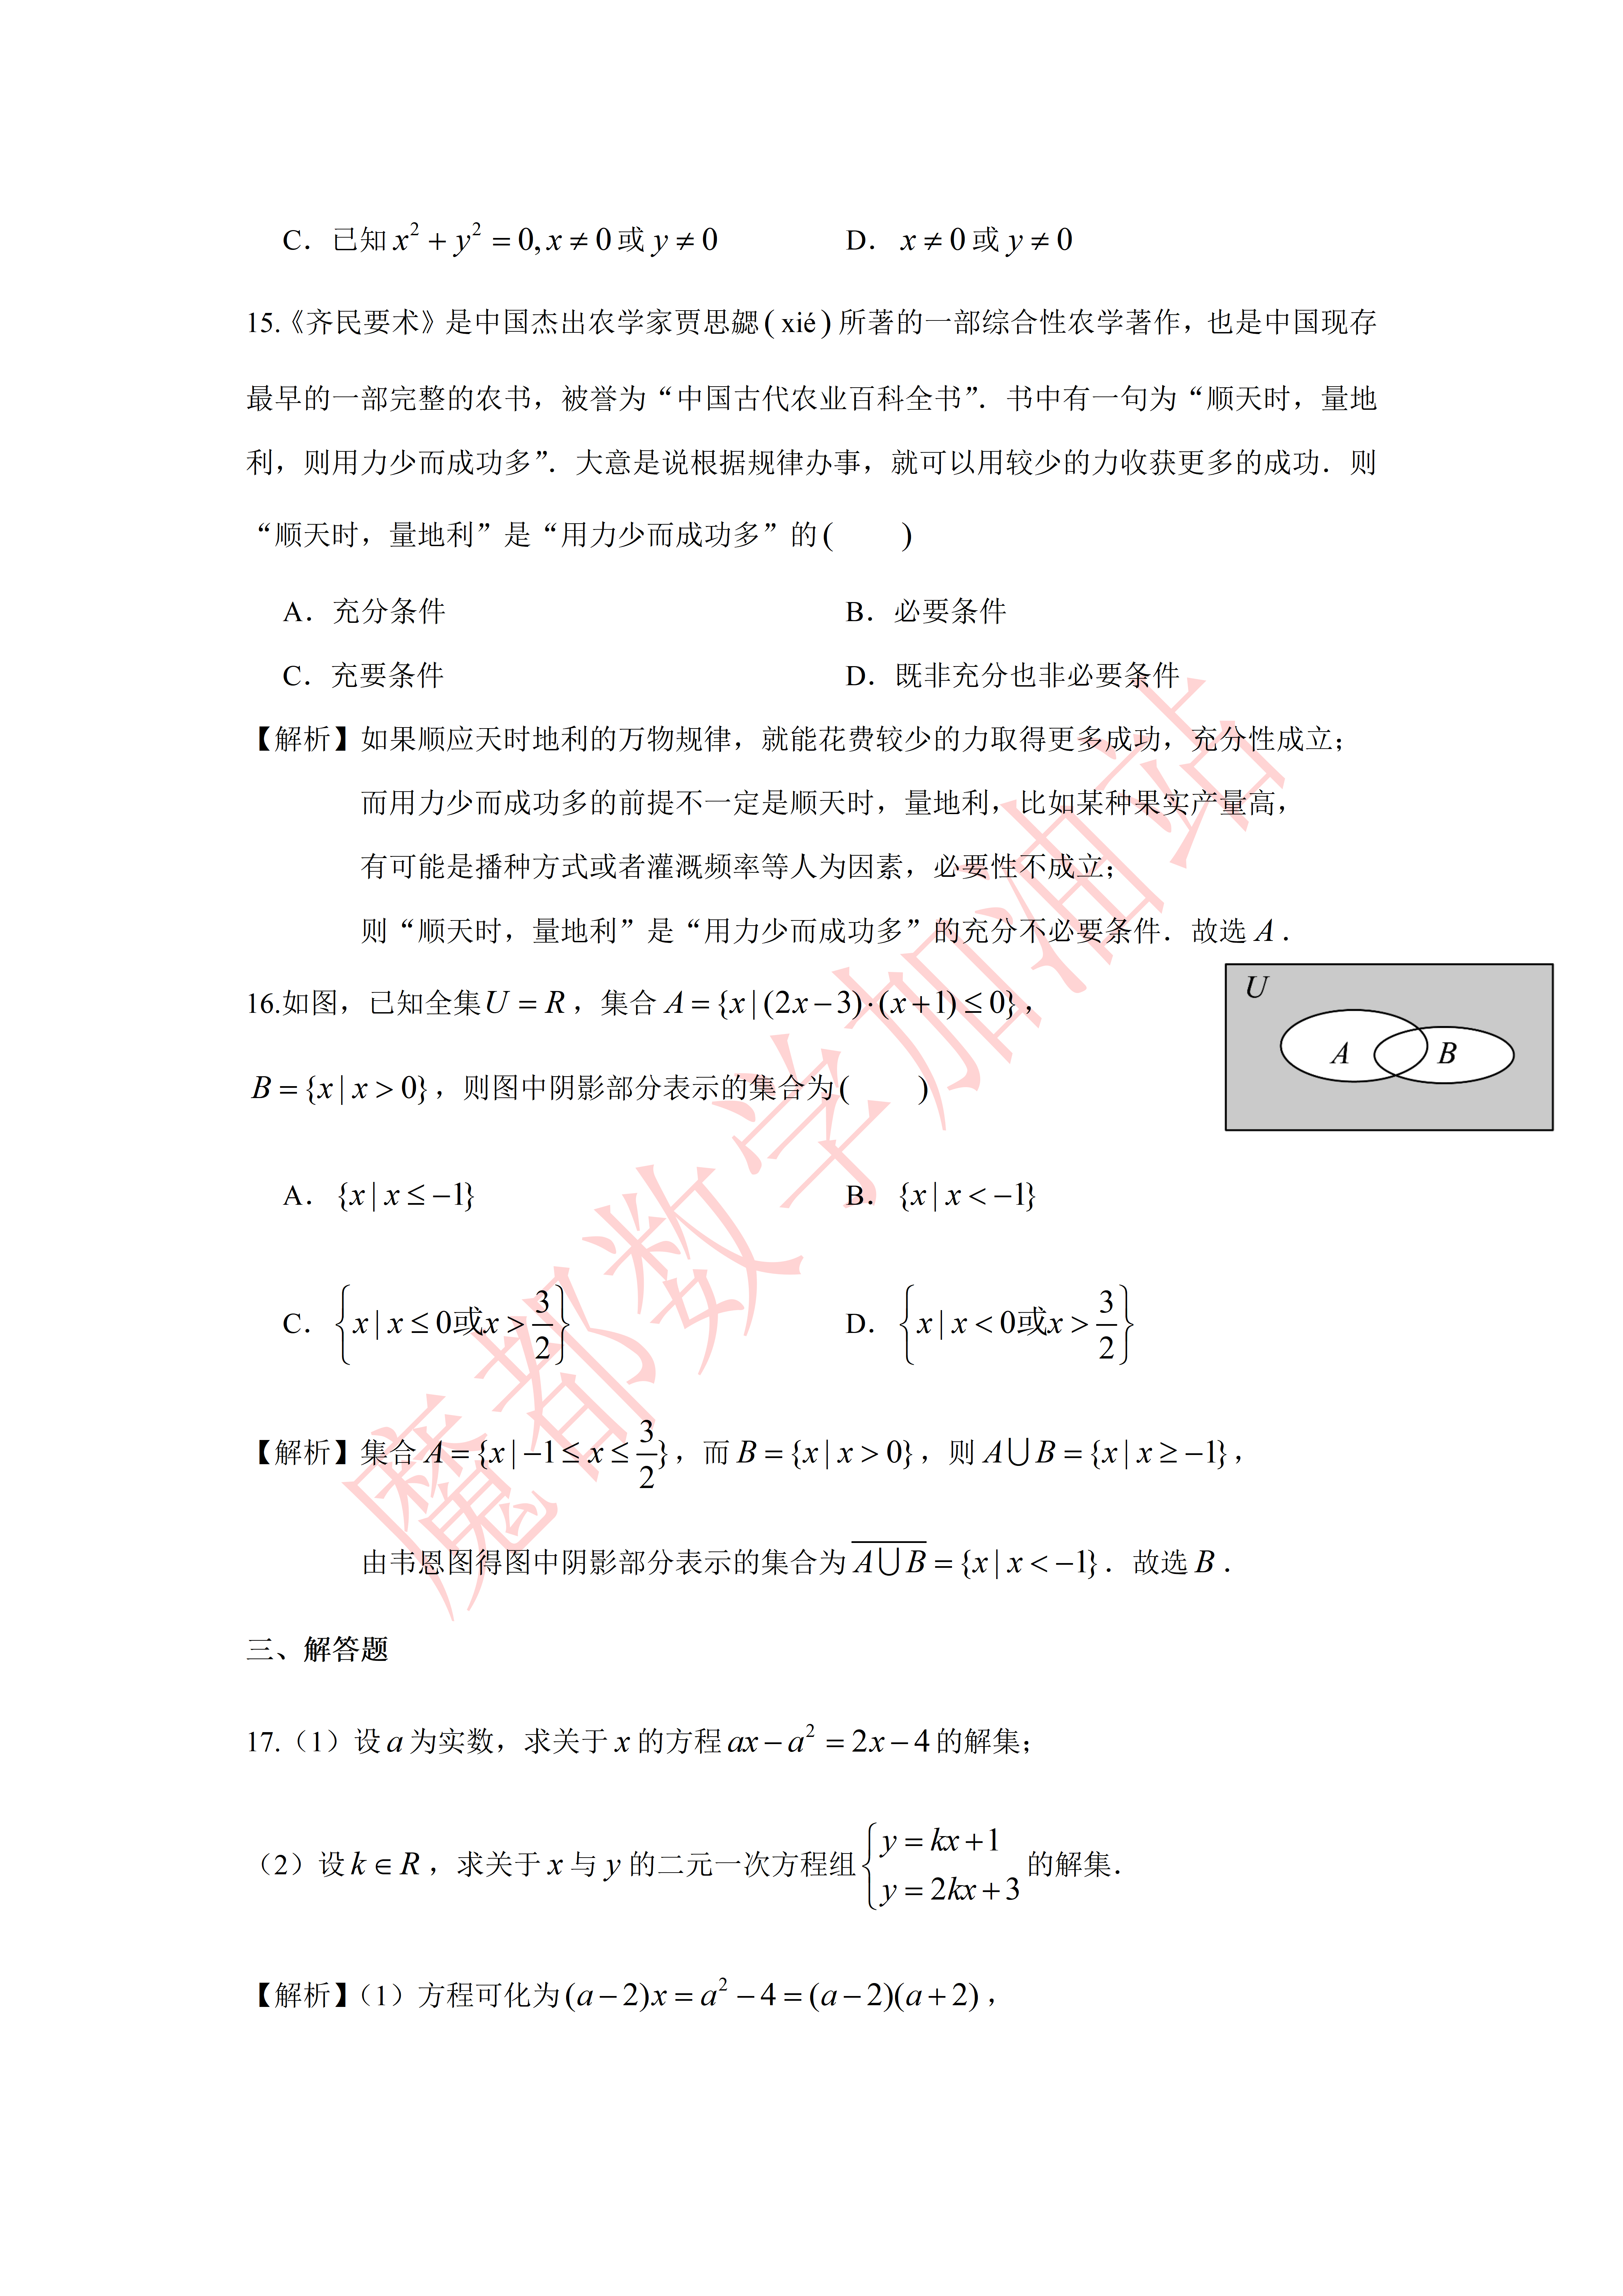
\includegraphics[width=.34\linewidth,trim=3586bp 3410bp 196bp 2818bp,clip]{../原图/高一52_回民中学_9月月考/04.png}
\end{center}

\keepwithprev
A. $\{x\mid x\leqslant-1\}$\qquad B. $\{x\mid x<-1\}$

C. $\left\{x\mid x\leqslant0\text{ 或 }x>\dfrac32\right\}$\qquad D. $\left\{x\mid x<0\text{ 或 }x>\dfrac32\right\}$

\ifanswer
\solbegin
\step{集合 $A=\left\{x\mid-1\leqslant x\leqslant\dfrac32\right\}$，而 $B=\{x\mid x>0\}$，则 $A\cup B=\{x\mid x\geqslant-1\}$，}
\step{由韦恩图得图中阴影部分表示的集合为 $\overline{A\cup B}=\{x\mid x<-1\}$．故选 $B$．}
\solend
\fi

\end{enumerate}

\bigsec{三、解答题}

\begin{enumerate}
\setcounter{enumi}{16}

\item （1）设 $a$ 为实数，求关于 $x$ 的方程 $ax-a^2=2x-4$ 的解集；

（2）设 $k\in\R$，求关于 $x$ 与 $y$ 的二元一次方程组 $\begin{cases}y=kx+1\\y=2kx+3\end{cases}$ 的解集．

\ifanswer
\solbegin
\stepm{(1)}{方程可化为 $(a-2)x=a^2-4=(a-2)(a+2)$，}
\step{当 $a\neq2$ 时，方程的解为 $x=\dfrac{(a-2)(a+2)}{a-2}=a+2$，则解集为 $\{a+2\}$；}
\step{当 $a=2$ 时，方程为 $2x-4=2x-4$，对 $x$ 取一切实数均成立，}
\step{所以解集为 $\R$；}
\stepm{(2)}{$\begin{cases}y=kx+1\\y=2kx+3\end{cases}$，则 $kx+1=2kx+3,kx=-2$，}
\step{当 $k=0$ 时，等式不成立，无解；当 $k\neq0$ 时，$x=-\dfrac2k,y=-1$；}
\step{综上所述，当 $k=0$ 时，解集为 $\varnothing$；当 $k\neq0$ 时，解集为 $\left\{\left(-\dfrac2k,-1\right)\right\}$．}
\solend
\fi

\ansspace[6]

\item 已知命题 $p$：方程 $x^2+6x+m-1=0$ 有两个不等的负根；命题 $q$：方程 $9x^2+6x+m-2=0$ 无实根．

\begin{enumerate}[label=(\arabic*)]
\item 若 $p$ 为真命题，求实数 $m$ 的取值范围；
\item 若 $p,q$ 两命题一真一假，求实数 $m$ 的取值范围．
\end{enumerate}

\ifanswer
\solbegin
\stepm{(1)}{设方程 $x^2+6x+m-1=0$ 两根为 $x_1,x_2$，}
\step{则 $\begin{cases}\Delta>0\\ x_1+x_2<0\\ x_1x_2>0\end{cases}\Rightarrow\begin{cases}36-4(m-1)>0\\ -6<0\\ m-1>0\end{cases}\Rightarrow1<m<10$；}
\stepm{(2)}{若命题 $q$ 为真命题，则 $36-36(m-2)<0\Rightarrow m>3$，}
\step{从而当命题 $q$ 为假命题时，$m\leqslant3$；}
\step{又由（1）得 $p$ 为假命题时，$m\leqslant1$ 或 $m\geqslant10$；}
\step{则当 $p$ 为真命题，$q$ 为假命题时，得 $\begin{cases}1<m<10\\ m\leqslant3\end{cases}\Rightarrow1<m\leqslant3$；}
\step{当 $q$ 为真命题，$p$ 为假命题时，得 $\begin{cases}m\leqslant1\text{ 或 }m\geqslant10\\ m>3\end{cases}\Rightarrow m\geqslant10$；}
\step{综上，当 $p,q$ 两命题一真一假时，$1<m\leqslant3$ 或 $m\geqslant10$.}
\solend
\fi

\ansspace[6]

\item 证明下列两个命题：

\begin{enumerate}[label=(\arabic*)]
\item 设 $ab>0$，求证：$a>b$ 是 $\dfrac1a<\dfrac1b$ 的充要条件．
\item 已知 $a,b$ 为正数，$n$ 为正整数，求证：如果 $a^n>b^n$，那么 $a>b$．
\end{enumerate}

\ifanswer
\solbegin
\stepm{(1)}{先证充分性：因为 $ab>0$ 且 $a>b$，故 $a-b>0$，从而 $\dfrac{a-b}{ab}>0$，}
\step{即 $\dfrac1b-\dfrac1a>0$，即 $\dfrac1a<\dfrac1b$；}
\step{再证必要性：若 $\dfrac1a<\dfrac1b$，则 $\dfrac1a-\dfrac1b=\dfrac{b-a}{ab}<0$，}
\step{又因为 $ab>0$，所以 $b-a<0$，即 $a>b$．}
% 原卷如此，照录未改（第 19 题(1)此句末用全角句号“。”，全卷其余各题末句用“．”，
% 见文件头“原卷笔误/存疑”第 4 条）
\step{综上，$a>b$ 是 $\dfrac1a<\dfrac1b$ 的充要条件。}
\stepm{(2)}{令 $f(x)=x^n,n\in\N^*$，则由幂函数的性质得 $f(x)$ 在第一象限是严格增的，}
\step{而 $a^n>b^n$ 即意味着 $f(a)>f(b)$，且 $a,b$ 为正数，从而 $a>b$．}
\solend
\fi

\ansspace[8]

\item （1）求关于 $x$ 的不等式 $(m-2)x>1-m$ 的解集；

（2）求关于 $x$ 的不等式 $x^2-(a+1)x+a\leqslant0$ 的解集．

\ifanswer
\solbegin
\stepm{(1)}{由不等式 $(m-2)x>1-m$，}
\step{当 $m-2>0$ 时，即 $m>2$ 时，解得 $x>\dfrac{1-m}{m-2}$，}
\step{所以不等式的解集为 $\left(\dfrac{1-m}{m-2},+\infty\right)$；}
\step{当 $m-2=0$ 时，即 $m=2$ 时，不等式即为 $0>-1$ 恒成立，}
\step{即不等式的解集为 $\R$；}
\step{当 $m-2<0$ 时，即 $m<2$ 时，解得 $x<\dfrac{1-m}{m-2}$，}
\step{所以不等式的解集为 $\left(-\infty,\dfrac{1-m}{m-2}\right)$；}
\step{综上，当 $m>2$ 时，解集为 $\left(\dfrac{1-m}{m-2},+\infty\right)$；}
\step{当 $m=2$ 时，解集为 $\R$；}
\step{当 $m<2$ 时，解集为 $\left(-\infty,\dfrac{1-m}{m-2}\right)$．}
\stepm{(2)}{由不等式 $x^2-(a+1)x+a\leqslant0$，可化为 $(x-a)(x-1)\leqslant0$，}
\step{当 $a>1$ 时，解得 $1\leqslant x\leqslant a$，即不等式的解集为 $[1,a]$；}
\step{当 $a=1$ 时，不等式即为 $(x-1)^2\leqslant0$，解得 $x=1$，即不等式的解集为 $\{1\}$；}
\step{当 $a<1$ 时，解得 $a\leqslant x\leqslant1$，即不等式的解集为 $[a,1]$，}
\step{综上，当 $a>1$ 时，解集为 $[1,a]$；}
\step{当 $a=1$ 时，解集为 $\{1\}$；}
\step{当 $a<1$ 时，解集为 $[a,1]$．}
\solend
\fi

\ansspace[10]

\item 已知集合 $A=\{x\mid(x+2)(5-x)\geqslant0\}$，若集合 $B$ 满足 $A\cap B=\varnothing,A\cup B=[-2,7)$．

\begin{enumerate}[label=(\arabic*)]
\item 用区间表示集合 $B$；
\item 若集合 $B$ 是不等式 $-x^2+bx+c>0$ 的解集，求实数 $b,c$ 的值；
\item 已知全集为 $\R$，若关于 $x$ 的不等式 $-1<x-a\leqslant2$ 的解集为 $M$，且“$x\in\overline A$”是“$x\in M$”的必要非充分条件，求实数 $a$ 的取值范围．
\end{enumerate}

\ifanswer
\solbegin
\stepm{(1)}{由题意得 $(x+2)(5-x)\geqslant0\Leftrightarrow(x+2)(x-5)\leqslant0\Rightarrow-2\leqslant x\leqslant5$，}
\step{则 $A=[-2,5]$，又 $A\cap B=\varnothing,A\cup B=[-2,7)$，则 $B=(5,7)$；}
\stepm{(2)}{$-x^2+bx+c>0\Leftrightarrow x^2-bx-c<0$，则 $x^2-bx-c=0$ 两根为 $5,7$，}
\step{则由韦达定理得 $b=12,-c=35\Rightarrow c=-35$；}
\stepm{(3)}{由题意得 $M=(a-1,a+2],\overline A=(-\infty,-2)\cup(5,+\infty)$，}
\step{且“$x\in\overline A$”是“$x\in M$”的必要非充分条件，则 $M$ 是 $\overline A$ 的真子集，}
\step{从而 $a+2<-2$ 或 $a-1\geqslant5$，解得 $a<-4$ 或 $a\geqslant6$，}
\step{所以实数 $a$ 的取值范围为 $(-\infty,-4)\cup[6,+\infty)$．}
\solend
\fi

\ansspace*[10]

\end{enumerate}

\end{document}
"
% 紧凑版：xelatex "\def\iscompact{1}% 高一52_回民中学_9月月考.tex
%   —— 高一上数学“2026-2027 年回民中学高一上 9 月月考”（讲评版）
% 试卷版：xelatex 高一52_回民中学_9月月考.tex
% 答案版：xelatex "\def\isanswer{1}\input{高一52_回民中学_9月月考.tex}"
% 紧凑版：xelatex "\def\iscompact{1}\input{高一52_回民中学_9月月考.tex}"
%
% 原始材料：微信公众号“魔都数学加油站”文章，作者破晓，连载“27学年高一52”；
% 原文标题“27学年高一52——2026-2027年上海市回民中学高一上9月月考”；
% 原文链接：https://mp.weixin.qq.com/s/ndjyozrRQCLl4ba3J8uR7g。
% 该页面用 JS 渲染，未见明确发布日期；页面内时间戳约为 2026-10-06 21:19／21:38，本稿以该时刻记可得日期。
% 正文为 8 张 PNG 页：第 01—07 页 4762×6735，第 08 页 2560×3620（**同一篇各页分辨率不同**），
% 均按页序读取。8 页全为试卷正文页（卷首标题在第 1 页页顶，卷末解答题第 21 题解析止于第 8 页），
% 无封面页、目录页、二维码或宣传页。粉色斜排“魔都数学加油站”为卷面水印，与公众号页脚一并未录入。
%
% 卷首标题：照卷面印作“2026--2027 年回民中学高一上 9 月月考”（公众号标题中的“上海市”
% 卷面标题行没有，本稿照卷面），年份区间按全稿惯例排 en dash。原卷只有一行标题、无副标题。
%
% 篇幅与题号：原卷自第 3 题起编号（第 1、2 题不在本卷内）。填空题 3—12（10 题）、
% 选择题 13—16（4 题）、解答题 17—21（5 题），共 19 题。本稿沿用原节与原题号，
% 只改排为全稿统一的大节样式（原卷小节标题为“一、填空题”“二、选择题”“三、解答题”）。
%
% 讲评版：原卷每题下直接印【答案】或【解析】。**只印【答案】的 1 题**（第 3 题），本稿只给 \ans{}；
% **第 14 题没有任何【答案】/【解析】段**，答案“D”直接印在题干括号内（“应假设(  D  )”），
% 本稿按 高一37 第 13 题的成例把括号留空、答案另提为 \ans{$D$}；
% 其余 17 题都只印【解析】，按全稿口径这类题不另提 \ans{}——其中选择题第 13、15、16 题的结论
% 写在解析末句（“故选 A／A／B”），亦照录在解析内。
%
% 副标题：原卷未印副标题。本稿按“知识模块”口径标作“集合与常用逻辑用语、不等式”：
% 19 题中集合与常用逻辑用语 10 题（集合类 7 题——第 3、4、5、9、12、16、21 题；
% 逻辑类 3 题——第 6、14、15 题），不等式 9 题（含等式性质与一元二次方程：第 7、8、10、11、
% 13、17、18、19、20 题），两类均远超三分之一，故并标。口径同 高一46、高一47、高一48、高一51。
%
% 与原卷的排版差异：
%   ① 原卷每题下直接印【答案】/【解析】，本稿按全稿惯例将答案与解析置于答案版，试卷版保持干净；
%      第 14 题印在题干括号内的答案“D”同样移入 \ans{}，见上；
%   ② 原卷未印副标题，本稿按“知识模块”口径补出；
%   ③ 原卷填空横线约两个字宽，本稿按全稿惯例统一排 \blankline[4.4em]；
%      选择题的作答括号原卷排半角“(    )”，本稿按全稿惯例排 \mbox{（\quad）}；
%   ④ 原卷实数集、自然数集排斜体/粗体 $R$、$\mathbf{R}$、$N$，本稿按全稿惯例改用 $\R$、$\N$；
%      空集记号统一为 \varnothing；
%   ⑤ 第 8 题题干与解析两处“两个实数分别为 $x_1$、$x_2$”原卷即用顿号，第 10、13 题等处
%      原卷在数学式内用半角逗号（如 $x_1,x_2$、$a,b,c\in R$），两份均照录未强改；
%      句末句点按全稿惯例排西文句点，句中句点（第 9、12、15、21 题）照原卷排全角“．”；
%   ⑥ 第 17、20 题原卷把子问标号“（1）”排在该题题号同一行，本稿照原卷仍排同一行（同 高一34 的
%      做法）；第 18、19、21 题的子问原卷各自另起一行，本稿按全稿惯例用 enumerate 的 (1)(2)(3)；
%      解析中的子问标号一律用 \stepm{(1)}{…}；
%   ⑦ 第 16 题的韦恩图原卷排在题干与选项右侧的浮动位置，本稿居中排在题干之后、选项之前，
%      并加 \needvspace 整块推走（守卫写在 \item 之前）；图自原图第 4 页裁切（trim），不另存图片文件；
%   ⑧ 每道解答题原卷未留作答空白，本稿按全稿惯例加 \ansspace。
%
% 原卷笔误/存疑（均照录未改，正文对应处另有 % 注）：
%   1. 第 8 题题干与解析首行两处均作“两个实数分别为 $x_1$、$x_2$”，按文意应为“两个实数**根**”
%      （疑脱“根”字，第 10 题同位置作“两个实根分别是”）；
%   2. 第 4 题解析“满足条件的 $A$ 的个数为集合 $\{0,1,3\}$ 的真子集，即 7 个”，
%      “个数为……真子集”表述不严（应为“……的真子集的个数”）；$\{0,1,3\}$ 的真子集 7 个，结论无误；
%   3. 第 6 题解析第 2 行“当 $a=10,b=0.2$ 时，$a+b>2$，且 $ab>1$，所以 $a>1$，且 $b>1$ 不成立”
%      ——此处是举反例，“所以”按文意应为“但”（$a=10,b=0.2$ 与“$a>1$ 且 $b>1$”不成立之间是转折，
%      非因果）；
%   4. 第 19 题 (1) 解析末行“综上，$a>b$ 是 $\dfrac1a<\dfrac1b$ 的充要条件。”用全角句号“。”，
%      全卷其余各题末句均用“．”，体例不一，照录；
%   5. 第 20 题第 (1) 问解析先按 $m>2$、$m=2$、$m<2$ 三种情况各给出解集，末三行又“综上”重述一遍，
%      与原卷一致（内容重复，非笔误）；
%   6. 第 18 题题干第 (2) 问“若 $p,q$ 两命题一真一假”，正文照录原卷所用半角逗号（未改顿号）。
%
% 插图：1 张，自原图裁切（无 \begin{tikzpicture} 重排）：
%   · 第 16 题题干韦恩图（全集 $U$ 矩形内两相交椭圆 $A$、$B$，灰色为阴影部分）
%     ——原图第 04 页，原卷排于题干与选项右侧。
%     裁框：x 3594–4558、y 2826–3317（即矩形外框，四周各留 4px），
%     trim=3590bp 3414bp 200bp 2822bp（左／下／右／上），页宽 4762、页高 6735。
%
\documentclass[a4paper,11pt]{article}
\usepackage{common}

\begin{document}

\examtitlest[3]{2026--2027 年回民中学高一上 9 月月考}{集合与常用逻辑用语、不等式}

\bigsec{一、填空题}

\begin{enumerate}
\setcounter{enumi}{2}

\item 用列举法写出下列集合 $\{(x,y)\mid x+y=2,x\in\N,y\in\N\}=$\blankline[4.4em].

\ifanswer
\ans{$\{(0,2),(1,1),(2,0)\}$}
\fi

\item 设集合 $A$ 满足 $\{-1,2\}\sub A\subset\{-1,0,1,2,3\}$，则满足条件的 $A$ 有\blankline[4.4em]个.

\ifanswer
\solbegin
\step{满足条件的 $A$ 的个数为集合 $\{0,1,3\}$ 的真子集，即 $7$ 个.}
\solend
\fi

\item 已知集合 $A=\{2,(a+1)^2,a^2+2\}$，且 $1\in A$，则实数 $a$ 的值为\blankline[4.4em].

\ifanswer
\solbegin
\step{因为 $1\in A$，而 $a^2+2\geqslant2$，所以 $(a+1)^2=1$，解得 $a=0$ 或 $a=-2$，}
\step{$a=0$ 时，$a^2+2=2$，不合题意，$a=-2$ 时，$a^2+2=6$，满足题意，}
\step{所以 $a=-2$.}
\solend
\fi

\item 已知 $a,b$ 是实数，则“$a>1$，且 $b>1$”是“$a+b>2$，且 $ab>1$”的\blankline[4.4em]条件.

\ifanswer
\solbegin
\step{$a,b$ 是实数，则“$a>1$，且 $b>1$”$\Rightarrow$“$a+b>2$，且 $ab>1$”正确，}
% 原卷如此，照录未改（第 6 题解析此处作“所以 $a>1$，且 $b>1$ 不成立”，按文意为转折，
% 见文件头“原卷笔误/存疑”第 3 条）
\step{当 $a=10,b=0.2$ 时，$a+b>2$，且 $ab>1$，所以 $a>1$，且 $b>1$ 不成立，}
\step{即前者是推出后者，后者推不出前者，}
\step{所以“$a>1$，且 $b>1$”是“$a+b>2$，且 $ab>1$”的充分而不必要条件.}
\solend
\fi

\item 已知等式 $2x^2-3x-1=a(x-1)^2+b(x-1)+c$ 恒成立，其中 $a,b,c$ 为常数，则 $a+b-c=$\blankline[4.4em].

\ifanswer
\solbegin
\step{将等式右侧展开整理得 $a(x-1)^2+b(x-1)+c=ax^2+(-2a+b)x+(a-b+c)$，}
\step{左右两边多项式恒等，对应次数的系数必须相等：}
\step{则 $a=2,-2a+b=-3$，代入 $a=2$ 得 $b=1$，$a-b+c=-1$，}
\step{代入 $a=2,b=1$ 得 $c=-2$，得 $a+b-c=2+1-(-2)=5$.}
\solend
\fi

% 原卷如此，照录未改（第 8 题题干与解析首行两处“两个实数分别为”疑脱“根”字，
% 见文件头“原卷笔误/存疑”第 1 条）
\item 若关于 $x$ 的二次方程 $x^2+mx+4m^2-3=0$ 的两个实数分别为 $x_1$、$x_2$，且满足 $x_1+x_2=x_1x_2$，则实数 $m$ 的值为\blankline[4.4em].

\ifanswer
\solbegin
% 原卷如此，照录未改（此处“两个实数分别为”同题干，疑脱“根”字）
\step{二次方程 $x^2+mx+4m^2-3=0$ 的两个实数分别为 $x_1$、$x_2$，}
\step{则有 $\Delta=m^2-4(4m^2-3)\geqslant0$，变形得 $m^2\leqslant\dfrac45$，}
\step{则 $x_1+x_2=-m$，$x_1x_2=(4m^2-3)$，}
\step{若 $x_1+x_2=x_1x_2$，则有 $-m=4m^2-3$，解得 $m=-1$ 或 $\dfrac34$，}
\step{又 $m^2\leqslant\dfrac45$，则 $m=\dfrac34$.}
\solend
\fi

\item 设集合 $A=\{x\mid x^2=1\}$，$B=\{x\mid ax=1\}$．若 $A\cap B=B$，则实数 $a$ 的值为\blankline[4.4em].

\ifanswer
\solbegin
\step{集合 $A=\{x\mid x^2=1\}=\{-1,1\}$，$B=\{x\mid ax=1\}$，$A\cap B=B$，所以 $B\sub A$，}
\step{当 $a=0$ 时，$B=\varnothing$，成立；}
\step{当 $a\neq0$ 时，$B=\left\{\dfrac1a\right\}$，则 $\dfrac1a=-1$ 或 $\dfrac1a=1$，解得 $a=-1$ 或 $a=1$，}
\step{所以实数 $a$ 的值为 $0$ 或 $1$ 或 $-1$.}
\solend
\fi

\item 已知关于 $x$ 的一元二次方程 $x^2+3x-3=0$ 的两个实根分别是 $x_1,x_2$，则以 $-\dfrac1{x_1},-\dfrac1{x_2}$ 为根且二次项系数是 $1$ 的一元二次方程为\blankline[4.4em].

\ifanswer
\solbegin
\step{因为 $x_1,x_2$ 是一元二次方程 $x^2+3x-3=0$ 的两个实根，}
\step{所以 $x_1+x_2=-3,x_1x_2=-3$，}
\step{所以 $-\dfrac1{x_1}+\left(-\dfrac1{x_2}\right)=-\dfrac{x_1+x_2}{x_1x_2}=-1$，$-\dfrac1{x_1}\cdot\left(-\dfrac1{x_2}\right)=\dfrac1{x_1x_2}=-\dfrac13$，}
\step{所以一元二次方程为 $x^2+x-\dfrac13=0$.}
\solend
\fi

\item 若关于 $x$ 的不等式 $(a-2)x^2+2(a-2)x-4<0$ 的解集是 $\R$，则实数 $a$ 的取值范围是\blankline[4.4em].

\ifanswer
\solbegin
\step{当 $a=2$ 时，不等式化为 $-4<0$ 对于任意实数 $x$ 都成立，因此 $a=2$ 满足题意；}
\step{当 $a\neq2$ 时，要使关于 $x$ 的不等式 $(a-2)x^2+2(a-2)x-4<0$ 的解集为 $\R$，}
\step{则 $\begin{cases}a-2<0\\ \Delta=4(a-2)^2+16(a-2)<0\end{cases}$，解得 $-2<a<2$．}
\step{综上，$a$ 的取值范围为 $(-2,2]$．}
\solend
\fi

\item 设非空集合 $A$、$B$，定义 $A\times B=\{x\mid x\in(A\cup B),x\notin(A\cap B)\}$．已知 $A=\{x\mid0\leqslant x\leqslant2\}$，$B=\{y\mid y\geqslant0\}$，则 $A\times B=$\blankline[4.4em].

\ifanswer
\solbegin
\step{由于 $A=\{x\mid0\leqslant x\leqslant2\}$，$B=\{y\mid y\geqslant0\}=\{x\mid x\geqslant0\}$，}
\step{所以 $A\cup B=\{x\mid x\geqslant0\}$，$A\cap B=\{x\mid0\leqslant x\leqslant2\}$，故 $A\times B=\{x\mid x>2\}$．}
\solend
\fi

\end{enumerate}

\bigsec{二、选择题}

\begin{enumerate}
\setcounter{enumi}{12}

\item 已知 $a,b,c\in\R$ 且 $a>b$，则下列不等式一定成立的是\mbox{（\quad）}

\keepwithprev
A. $\dfrac{a}{c^2+1}>\dfrac{b}{c^2+1}$\qquad B. $\dfrac1a<\dfrac1b$

C. $ac>bc$\qquad D. $a^2>b^2$

\ifanswer
\solbegin
\step{对于 A：因为 $c^2+1>0$ 恒成立，且 $a>b$，所以 $\dfrac{a}{c^2+1}>\dfrac{b}{c^2+1}$ 一定成立，}
\step{所以 A 正确；}
\step{对于 B：当 $a=1,b=-1$ 时，满足 $a>b$，此时 $\dfrac1a=1>\dfrac1b=-1$，所以 B 错误；}
\step{对于 C：当 $c<0$ 时，由 $a>b$，得 $ac<bc$，所以 C 错误；}
\step{对于 D：当 $a=1,b=-2$ 时，满足 $a>b$，此时 $a^2=1<b^2=4$，所以 D 错误；}
\step{故选 $A$．}
\solend
\fi

% 注：本题的答案“D”原卷直接印在题干末尾的括号内（“应假设(  D  )”），且没有单独的
%     【答案】/【解析】段，本稿按 高一37 第 13 题的成例把括号留空、另提为 \ans{}，
%     见文件头“与原卷的排版差异”①。
\item 用反证法证明：“已知 $x,y\in\R$,$x^2+y^2=0$，求证：$x=y=0$”时，应假设\mbox{（\quad）}

\keepwithprev
A. 已知 $x^2+y^2=0,x\neq0$ 且 $y\neq0$\qquad B. $x\neq0$ 且 $y\neq0$

C. 已知 $x^2+y^2=0,x\neq0$ 或 $y\neq0$\qquad D. $x\neq0$ 或 $y\neq0$

\ans{$D$}

\item 《齐民要术》是中国杰出农学家贾思勰（xié）所著的一部综合性农学著作，也是中国现存最早的一部完整的农书，被誉为“中国古代农业百科全书”．书中有一句为“顺天时，量地利，则用力少而成功多”．大意是说根据规律办事，就可以用较少的力收获更多的成功．则“顺天时，量地利”是“用力少而成功多”的\mbox{（\quad）}

\keepwithprev
A. 充分条件\qquad B. 必要条件

C. 充要条件\qquad D. 既非充分也非必要条件

\ifanswer
\solbegin
\step{如果顺应天时地利的万物规律，就能花费较少的力取得更多成功，充分性成立；}
\step{而用力少而成功多的前提不一定是顺天时，量地利，比如某种果实产量高，}
\step{有可能是播种方式或者灌溉频率等人为因素，必要性不成立；}
\step{则“顺天时，量地利”是“用力少而成功多”的充分不必要条件．故选 $A$．}
\solend
\fi

\needvspace{13\baselineskip}

\item 如图，已知全集 $U=\R$，集合 $A=\{x\mid(2x-3)\cdot(x+1)\leqslant0\}$，$B=\{x\mid x>0\}$，则图中阴影部分表示的集合为\mbox{（\quad）}

\begin{center}
% 原图第 4 页题干韦恩图直接裁取（原卷排于题干与选项右侧）。
% 裁框取矩形外框 x 3590–4558、y 2822–3321，再向外各留 4px（即 x 3586–4562、y 2818–3325），
% trim=左 3586bp／下 3410bp／右 196bp／上 2818bp（页宽 4762、页高 6735）。
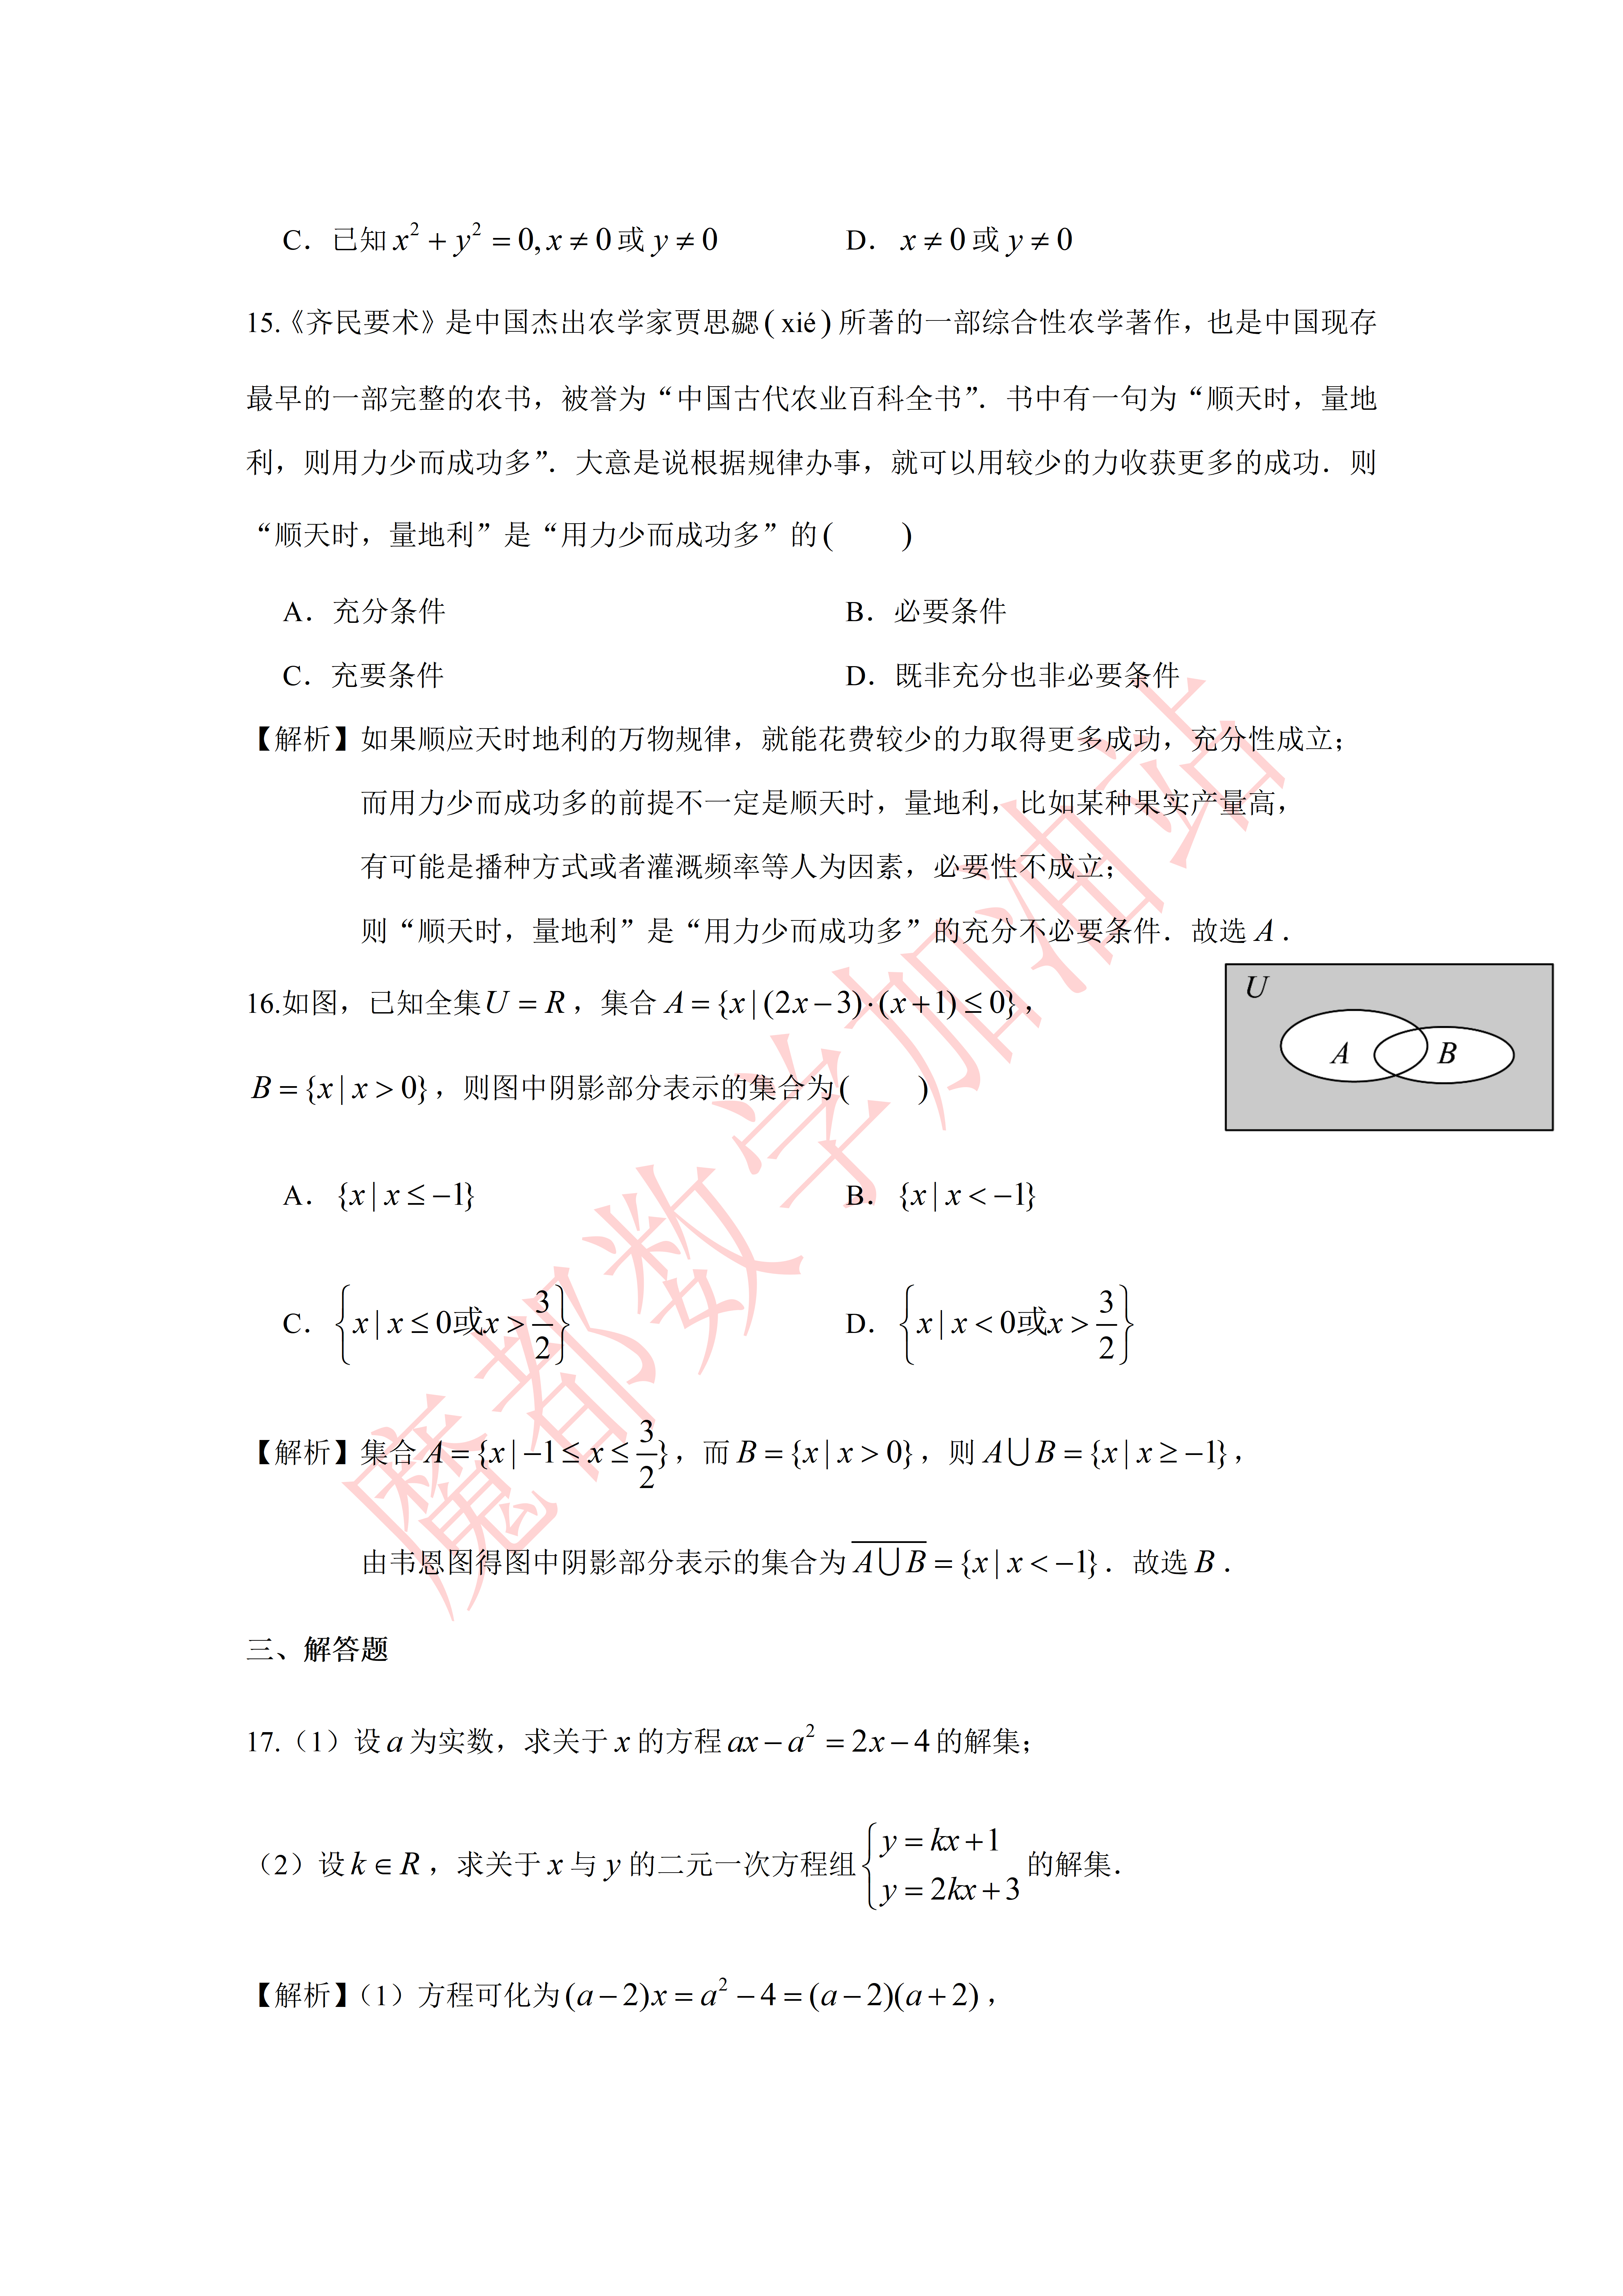
\includegraphics[width=.34\linewidth,trim=3586bp 3410bp 196bp 2818bp,clip]{../原图/高一52_回民中学_9月月考/04.png}
\end{center}

\keepwithprev
A. $\{x\mid x\leqslant-1\}$\qquad B. $\{x\mid x<-1\}$

C. $\left\{x\mid x\leqslant0\text{ 或 }x>\dfrac32\right\}$\qquad D. $\left\{x\mid x<0\text{ 或 }x>\dfrac32\right\}$

\ifanswer
\solbegin
\step{集合 $A=\left\{x\mid-1\leqslant x\leqslant\dfrac32\right\}$，而 $B=\{x\mid x>0\}$，则 $A\cup B=\{x\mid x\geqslant-1\}$，}
\step{由韦恩图得图中阴影部分表示的集合为 $\overline{A\cup B}=\{x\mid x<-1\}$．故选 $B$．}
\solend
\fi

\end{enumerate}

\bigsec{三、解答题}

\begin{enumerate}
\setcounter{enumi}{16}

\item （1）设 $a$ 为实数，求关于 $x$ 的方程 $ax-a^2=2x-4$ 的解集；

（2）设 $k\in\R$，求关于 $x$ 与 $y$ 的二元一次方程组 $\begin{cases}y=kx+1\\y=2kx+3\end{cases}$ 的解集．

\ifanswer
\solbegin
\stepm{(1)}{方程可化为 $(a-2)x=a^2-4=(a-2)(a+2)$，}
\step{当 $a\neq2$ 时，方程的解为 $x=\dfrac{(a-2)(a+2)}{a-2}=a+2$，则解集为 $\{a+2\}$；}
\step{当 $a=2$ 时，方程为 $2x-4=2x-4$，对 $x$ 取一切实数均成立，}
\step{所以解集为 $\R$；}
\stepm{(2)}{$\begin{cases}y=kx+1\\y=2kx+3\end{cases}$，则 $kx+1=2kx+3,kx=-2$，}
\step{当 $k=0$ 时，等式不成立，无解；当 $k\neq0$ 时，$x=-\dfrac2k,y=-1$；}
\step{综上所述，当 $k=0$ 时，解集为 $\varnothing$；当 $k\neq0$ 时，解集为 $\left\{\left(-\dfrac2k,-1\right)\right\}$．}
\solend
\fi

\ansspace[6]

\item 已知命题 $p$：方程 $x^2+6x+m-1=0$ 有两个不等的负根；命题 $q$：方程 $9x^2+6x+m-2=0$ 无实根．

\begin{enumerate}[label=(\arabic*)]
\item 若 $p$ 为真命题，求实数 $m$ 的取值范围；
\item 若 $p,q$ 两命题一真一假，求实数 $m$ 的取值范围．
\end{enumerate}

\ifanswer
\solbegin
\stepm{(1)}{设方程 $x^2+6x+m-1=0$ 两根为 $x_1,x_2$，}
\step{则 $\begin{cases}\Delta>0\\ x_1+x_2<0\\ x_1x_2>0\end{cases}\Rightarrow\begin{cases}36-4(m-1)>0\\ -6<0\\ m-1>0\end{cases}\Rightarrow1<m<10$；}
\stepm{(2)}{若命题 $q$ 为真命题，则 $36-36(m-2)<0\Rightarrow m>3$，}
\step{从而当命题 $q$ 为假命题时，$m\leqslant3$；}
\step{又由（1）得 $p$ 为假命题时，$m\leqslant1$ 或 $m\geqslant10$；}
\step{则当 $p$ 为真命题，$q$ 为假命题时，得 $\begin{cases}1<m<10\\ m\leqslant3\end{cases}\Rightarrow1<m\leqslant3$；}
\step{当 $q$ 为真命题，$p$ 为假命题时，得 $\begin{cases}m\leqslant1\text{ 或 }m\geqslant10\\ m>3\end{cases}\Rightarrow m\geqslant10$；}
\step{综上，当 $p,q$ 两命题一真一假时，$1<m\leqslant3$ 或 $m\geqslant10$.}
\solend
\fi

\ansspace[6]

\item 证明下列两个命题：

\begin{enumerate}[label=(\arabic*)]
\item 设 $ab>0$，求证：$a>b$ 是 $\dfrac1a<\dfrac1b$ 的充要条件．
\item 已知 $a,b$ 为正数，$n$ 为正整数，求证：如果 $a^n>b^n$，那么 $a>b$．
\end{enumerate}

\ifanswer
\solbegin
\stepm{(1)}{先证充分性：因为 $ab>0$ 且 $a>b$，故 $a-b>0$，从而 $\dfrac{a-b}{ab}>0$，}
\step{即 $\dfrac1b-\dfrac1a>0$，即 $\dfrac1a<\dfrac1b$；}
\step{再证必要性：若 $\dfrac1a<\dfrac1b$，则 $\dfrac1a-\dfrac1b=\dfrac{b-a}{ab}<0$，}
\step{又因为 $ab>0$，所以 $b-a<0$，即 $a>b$．}
% 原卷如此，照录未改（第 19 题(1)此句末用全角句号“。”，全卷其余各题末句用“．”，
% 见文件头“原卷笔误/存疑”第 4 条）
\step{综上，$a>b$ 是 $\dfrac1a<\dfrac1b$ 的充要条件。}
\stepm{(2)}{令 $f(x)=x^n,n\in\N^*$，则由幂函数的性质得 $f(x)$ 在第一象限是严格增的，}
\step{而 $a^n>b^n$ 即意味着 $f(a)>f(b)$，且 $a,b$ 为正数，从而 $a>b$．}
\solend
\fi

\ansspace[8]

\item （1）求关于 $x$ 的不等式 $(m-2)x>1-m$ 的解集；

（2）求关于 $x$ 的不等式 $x^2-(a+1)x+a\leqslant0$ 的解集．

\ifanswer
\solbegin
\stepm{(1)}{由不等式 $(m-2)x>1-m$，}
\step{当 $m-2>0$ 时，即 $m>2$ 时，解得 $x>\dfrac{1-m}{m-2}$，}
\step{所以不等式的解集为 $\left(\dfrac{1-m}{m-2},+\infty\right)$；}
\step{当 $m-2=0$ 时，即 $m=2$ 时，不等式即为 $0>-1$ 恒成立，}
\step{即不等式的解集为 $\R$；}
\step{当 $m-2<0$ 时，即 $m<2$ 时，解得 $x<\dfrac{1-m}{m-2}$，}
\step{所以不等式的解集为 $\left(-\infty,\dfrac{1-m}{m-2}\right)$；}
\step{综上，当 $m>2$ 时，解集为 $\left(\dfrac{1-m}{m-2},+\infty\right)$；}
\step{当 $m=2$ 时，解集为 $\R$；}
\step{当 $m<2$ 时，解集为 $\left(-\infty,\dfrac{1-m}{m-2}\right)$．}
\stepm{(2)}{由不等式 $x^2-(a+1)x+a\leqslant0$，可化为 $(x-a)(x-1)\leqslant0$，}
\step{当 $a>1$ 时，解得 $1\leqslant x\leqslant a$，即不等式的解集为 $[1,a]$；}
\step{当 $a=1$ 时，不等式即为 $(x-1)^2\leqslant0$，解得 $x=1$，即不等式的解集为 $\{1\}$；}
\step{当 $a<1$ 时，解得 $a\leqslant x\leqslant1$，即不等式的解集为 $[a,1]$，}
\step{综上，当 $a>1$ 时，解集为 $[1,a]$；}
\step{当 $a=1$ 时，解集为 $\{1\}$；}
\step{当 $a<1$ 时，解集为 $[a,1]$．}
\solend
\fi

\ansspace[10]

\item 已知集合 $A=\{x\mid(x+2)(5-x)\geqslant0\}$，若集合 $B$ 满足 $A\cap B=\varnothing,A\cup B=[-2,7)$．

\begin{enumerate}[label=(\arabic*)]
\item 用区间表示集合 $B$；
\item 若集合 $B$ 是不等式 $-x^2+bx+c>0$ 的解集，求实数 $b,c$ 的值；
\item 已知全集为 $\R$，若关于 $x$ 的不等式 $-1<x-a\leqslant2$ 的解集为 $M$，且“$x\in\overline A$”是“$x\in M$”的必要非充分条件，求实数 $a$ 的取值范围．
\end{enumerate}

\ifanswer
\solbegin
\stepm{(1)}{由题意得 $(x+2)(5-x)\geqslant0\Leftrightarrow(x+2)(x-5)\leqslant0\Rightarrow-2\leqslant x\leqslant5$，}
\step{则 $A=[-2,5]$，又 $A\cap B=\varnothing,A\cup B=[-2,7)$，则 $B=(5,7)$；}
\stepm{(2)}{$-x^2+bx+c>0\Leftrightarrow x^2-bx-c<0$，则 $x^2-bx-c=0$ 两根为 $5,7$，}
\step{则由韦达定理得 $b=12,-c=35\Rightarrow c=-35$；}
\stepm{(3)}{由题意得 $M=(a-1,a+2],\overline A=(-\infty,-2)\cup(5,+\infty)$，}
\step{且“$x\in\overline A$”是“$x\in M$”的必要非充分条件，则 $M$ 是 $\overline A$ 的真子集，}
\step{从而 $a+2<-2$ 或 $a-1\geqslant5$，解得 $a<-4$ 或 $a\geqslant6$，}
\step{所以实数 $a$ 的取值范围为 $(-\infty,-4)\cup[6,+\infty)$．}
\solend
\fi

\ansspace*[10]

\end{enumerate}

\end{document}
"
%
% 原始材料：微信公众号“魔都数学加油站”文章，作者破晓，连载“27学年高一52”；
% 原文标题“27学年高一52——2026-2027年上海市回民中学高一上9月月考”；
% 原文链接：https://mp.weixin.qq.com/s/ndjyozrRQCLl4ba3J8uR7g。
% 该页面用 JS 渲染，未见明确发布日期；页面内时间戳约为 2026-10-06 21:19／21:38，本稿以该时刻记可得日期。
% 正文为 8 张 PNG 页：第 01—07 页 4762×6735，第 08 页 2560×3620（**同一篇各页分辨率不同**），
% 均按页序读取。8 页全为试卷正文页（卷首标题在第 1 页页顶，卷末解答题第 21 题解析止于第 8 页），
% 无封面页、目录页、二维码或宣传页。粉色斜排“魔都数学加油站”为卷面水印，与公众号页脚一并未录入。
%
% 卷首标题：照卷面印作“2026--2027 年回民中学高一上 9 月月考”（公众号标题中的“上海市”
% 卷面标题行没有，本稿照卷面），年份区间按全稿惯例排 en dash。原卷只有一行标题、无副标题。
%
% 篇幅与题号：原卷自第 3 题起编号（第 1、2 题不在本卷内）。填空题 3—12（10 题）、
% 选择题 13—16（4 题）、解答题 17—21（5 题），共 19 题。本稿沿用原节与原题号，
% 只改排为全稿统一的大节样式（原卷小节标题为“一、填空题”“二、选择题”“三、解答题”）。
%
% 讲评版：原卷每题下直接印【答案】或【解析】。**只印【答案】的 1 题**（第 3 题），本稿只给 \ans{}；
% **第 14 题没有任何【答案】/【解析】段**，答案“D”直接印在题干括号内（“应假设(  D  )”），
% 本稿按 高一37 第 13 题的成例把括号留空、答案另提为 \ans{$D$}；
% 其余 17 题都只印【解析】，按全稿口径这类题不另提 \ans{}——其中选择题第 13、15、16 题的结论
% 写在解析末句（“故选 A／A／B”），亦照录在解析内。
%
% 副标题：原卷未印副标题。本稿按“知识模块”口径标作“集合与常用逻辑用语、不等式”：
% 19 题中集合与常用逻辑用语 10 题（集合类 7 题——第 3、4、5、9、12、16、21 题；
% 逻辑类 3 题——第 6、14、15 题），不等式 9 题（含等式性质与一元二次方程：第 7、8、10、11、
% 13、17、18、19、20 题），两类均远超三分之一，故并标。口径同 高一46、高一47、高一48、高一51。
%
% 与原卷的排版差异：
%   ① 原卷每题下直接印【答案】/【解析】，本稿按全稿惯例将答案与解析置于答案版，试卷版保持干净；
%      第 14 题印在题干括号内的答案“D”同样移入 \ans{}，见上；
%   ② 原卷未印副标题，本稿按“知识模块”口径补出；
%   ③ 原卷填空横线约两个字宽，本稿按全稿惯例统一排 \blankline[4.4em]；
%      选择题的作答括号原卷排半角“(    )”，本稿按全稿惯例排 \mbox{（\quad）}；
%   ④ 原卷实数集、自然数集排斜体/粗体 $R$、$\mathbf{R}$、$N$，本稿按全稿惯例改用 $\R$、$\N$；
%      空集记号统一为 \varnothing；
%   ⑤ 第 8 题题干与解析两处“两个实数分别为 $x_1$、$x_2$”原卷即用顿号，第 10、13 题等处
%      原卷在数学式内用半角逗号（如 $x_1,x_2$、$a,b,c\in R$），两份均照录未强改；
%      句末句点按全稿惯例排西文句点，句中句点（第 9、12、15、21 题）照原卷排全角“．”；
%   ⑥ 第 17、20 题原卷把子问标号“（1）”排在该题题号同一行，本稿照原卷仍排同一行（同 高一34 的
%      做法）；第 18、19、21 题的子问原卷各自另起一行，本稿按全稿惯例用 enumerate 的 (1)(2)(3)；
%      解析中的子问标号一律用 \stepm{(1)}{…}；
%   ⑦ 第 16 题的韦恩图原卷排在题干与选项右侧的浮动位置，本稿居中排在题干之后、选项之前，
%      并加 \needvspace 整块推走（守卫写在 \item 之前）；图自原图第 4 页裁切（trim），不另存图片文件；
%   ⑧ 每道解答题原卷未留作答空白，本稿按全稿惯例加 \ansspace。
%
% 原卷笔误/存疑（均照录未改，正文对应处另有 % 注）：
%   1. 第 8 题题干与解析首行两处均作“两个实数分别为 $x_1$、$x_2$”，按文意应为“两个实数**根**”
%      （疑脱“根”字，第 10 题同位置作“两个实根分别是”）；
%   2. 第 4 题解析“满足条件的 $A$ 的个数为集合 $\{0,1,3\}$ 的真子集，即 7 个”，
%      “个数为……真子集”表述不严（应为“……的真子集的个数”）；$\{0,1,3\}$ 的真子集 7 个，结论无误；
%   3. 第 6 题解析第 2 行“当 $a=10,b=0.2$ 时，$a+b>2$，且 $ab>1$，所以 $a>1$，且 $b>1$ 不成立”
%      ——此处是举反例，“所以”按文意应为“但”（$a=10,b=0.2$ 与“$a>1$ 且 $b>1$”不成立之间是转折，
%      非因果）；
%   4. 第 19 题 (1) 解析末行“综上，$a>b$ 是 $\dfrac1a<\dfrac1b$ 的充要条件。”用全角句号“。”，
%      全卷其余各题末句均用“．”，体例不一，照录；
%   5. 第 20 题第 (1) 问解析先按 $m>2$、$m=2$、$m<2$ 三种情况各给出解集，末三行又“综上”重述一遍，
%      与原卷一致（内容重复，非笔误）；
%   6. 第 18 题题干第 (2) 问“若 $p,q$ 两命题一真一假”，正文照录原卷所用半角逗号（未改顿号）。
%
% 插图：1 张，自原图裁切（无 \begin{tikzpicture} 重排）：
%   · 第 16 题题干韦恩图（全集 $U$ 矩形内两相交椭圆 $A$、$B$，灰色为阴影部分）
%     ——原图第 04 页，原卷排于题干与选项右侧。
%     裁框：x 3594–4558、y 2826–3317（即矩形外框，四周各留 4px），
%     trim=3590bp 3414bp 200bp 2822bp（左／下／右／上），页宽 4762、页高 6735。
%
\documentclass[a4paper,11pt]{article}
\usepackage{common}

\begin{document}

\examtitlest[3]{2026--2027 年回民中学高一上 9 月月考}{集合与常用逻辑用语、不等式}

\bigsec{一、填空题}

\begin{enumerate}
\setcounter{enumi}{2}

\item 用列举法写出下列集合 $\{(x,y)\mid x+y=2,x\in\N,y\in\N\}=$\blankline[4.4em].

\ifanswer
\ans{$\{(0,2),(1,1),(2,0)\}$}
\fi

\item 设集合 $A$ 满足 $\{-1,2\}\sub A\subset\{-1,0,1,2,3\}$，则满足条件的 $A$ 有\blankline[4.4em]个.

\ifanswer
\solbegin
\step{满足条件的 $A$ 的个数为集合 $\{0,1,3\}$ 的真子集，即 $7$ 个.}
\solend
\fi

\item 已知集合 $A=\{2,(a+1)^2,a^2+2\}$，且 $1\in A$，则实数 $a$ 的值为\blankline[4.4em].

\ifanswer
\solbegin
\step{因为 $1\in A$，而 $a^2+2\geqslant2$，所以 $(a+1)^2=1$，解得 $a=0$ 或 $a=-2$，}
\step{$a=0$ 时，$a^2+2=2$，不合题意，$a=-2$ 时，$a^2+2=6$，满足题意，}
\step{所以 $a=-2$.}
\solend
\fi

\item 已知 $a,b$ 是实数，则“$a>1$，且 $b>1$”是“$a+b>2$，且 $ab>1$”的\blankline[4.4em]条件.

\ifanswer
\solbegin
\step{$a,b$ 是实数，则“$a>1$，且 $b>1$”$\Rightarrow$“$a+b>2$，且 $ab>1$”正确，}
% 原卷如此，照录未改（第 6 题解析此处作“所以 $a>1$，且 $b>1$ 不成立”，按文意为转折，
% 见文件头“原卷笔误/存疑”第 3 条）
\step{当 $a=10,b=0.2$ 时，$a+b>2$，且 $ab>1$，所以 $a>1$，且 $b>1$ 不成立，}
\step{即前者是推出后者，后者推不出前者，}
\step{所以“$a>1$，且 $b>1$”是“$a+b>2$，且 $ab>1$”的充分而不必要条件.}
\solend
\fi

\item 已知等式 $2x^2-3x-1=a(x-1)^2+b(x-1)+c$ 恒成立，其中 $a,b,c$ 为常数，则 $a+b-c=$\blankline[4.4em].

\ifanswer
\solbegin
\step{将等式右侧展开整理得 $a(x-1)^2+b(x-1)+c=ax^2+(-2a+b)x+(a-b+c)$，}
\step{左右两边多项式恒等，对应次数的系数必须相等：}
\step{则 $a=2,-2a+b=-3$，代入 $a=2$ 得 $b=1$，$a-b+c=-1$，}
\step{代入 $a=2,b=1$ 得 $c=-2$，得 $a+b-c=2+1-(-2)=5$.}
\solend
\fi

% 原卷如此，照录未改（第 8 题题干与解析首行两处“两个实数分别为”疑脱“根”字，
% 见文件头“原卷笔误/存疑”第 1 条）
\item 若关于 $x$ 的二次方程 $x^2+mx+4m^2-3=0$ 的两个实数分别为 $x_1$、$x_2$，且满足 $x_1+x_2=x_1x_2$，则实数 $m$ 的值为\blankline[4.4em].

\ifanswer
\solbegin
% 原卷如此，照录未改（此处“两个实数分别为”同题干，疑脱“根”字）
\step{二次方程 $x^2+mx+4m^2-3=0$ 的两个实数分别为 $x_1$、$x_2$，}
\step{则有 $\Delta=m^2-4(4m^2-3)\geqslant0$，变形得 $m^2\leqslant\dfrac45$，}
\step{则 $x_1+x_2=-m$，$x_1x_2=(4m^2-3)$，}
\step{若 $x_1+x_2=x_1x_2$，则有 $-m=4m^2-3$，解得 $m=-1$ 或 $\dfrac34$，}
\step{又 $m^2\leqslant\dfrac45$，则 $m=\dfrac34$.}
\solend
\fi

\item 设集合 $A=\{x\mid x^2=1\}$，$B=\{x\mid ax=1\}$．若 $A\cap B=B$，则实数 $a$ 的值为\blankline[4.4em].

\ifanswer
\solbegin
\step{集合 $A=\{x\mid x^2=1\}=\{-1,1\}$，$B=\{x\mid ax=1\}$，$A\cap B=B$，所以 $B\sub A$，}
\step{当 $a=0$ 时，$B=\varnothing$，成立；}
\step{当 $a\neq0$ 时，$B=\left\{\dfrac1a\right\}$，则 $\dfrac1a=-1$ 或 $\dfrac1a=1$，解得 $a=-1$ 或 $a=1$，}
\step{所以实数 $a$ 的值为 $0$ 或 $1$ 或 $-1$.}
\solend
\fi

\item 已知关于 $x$ 的一元二次方程 $x^2+3x-3=0$ 的两个实根分别是 $x_1,x_2$，则以 $-\dfrac1{x_1},-\dfrac1{x_2}$ 为根且二次项系数是 $1$ 的一元二次方程为\blankline[4.4em].

\ifanswer
\solbegin
\step{因为 $x_1,x_2$ 是一元二次方程 $x^2+3x-3=0$ 的两个实根，}
\step{所以 $x_1+x_2=-3,x_1x_2=-3$，}
\step{所以 $-\dfrac1{x_1}+\left(-\dfrac1{x_2}\right)=-\dfrac{x_1+x_2}{x_1x_2}=-1$，$-\dfrac1{x_1}\cdot\left(-\dfrac1{x_2}\right)=\dfrac1{x_1x_2}=-\dfrac13$，}
\step{所以一元二次方程为 $x^2+x-\dfrac13=0$.}
\solend
\fi

\item 若关于 $x$ 的不等式 $(a-2)x^2+2(a-2)x-4<0$ 的解集是 $\R$，则实数 $a$ 的取值范围是\blankline[4.4em].

\ifanswer
\solbegin
\step{当 $a=2$ 时，不等式化为 $-4<0$ 对于任意实数 $x$ 都成立，因此 $a=2$ 满足题意；}
\step{当 $a\neq2$ 时，要使关于 $x$ 的不等式 $(a-2)x^2+2(a-2)x-4<0$ 的解集为 $\R$，}
\step{则 $\begin{cases}a-2<0\\ \Delta=4(a-2)^2+16(a-2)<0\end{cases}$，解得 $-2<a<2$．}
\step{综上，$a$ 的取值范围为 $(-2,2]$．}
\solend
\fi

\item 设非空集合 $A$、$B$，定义 $A\times B=\{x\mid x\in(A\cup B),x\notin(A\cap B)\}$．已知 $A=\{x\mid0\leqslant x\leqslant2\}$，$B=\{y\mid y\geqslant0\}$，则 $A\times B=$\blankline[4.4em].

\ifanswer
\solbegin
\step{由于 $A=\{x\mid0\leqslant x\leqslant2\}$，$B=\{y\mid y\geqslant0\}=\{x\mid x\geqslant0\}$，}
\step{所以 $A\cup B=\{x\mid x\geqslant0\}$，$A\cap B=\{x\mid0\leqslant x\leqslant2\}$，故 $A\times B=\{x\mid x>2\}$．}
\solend
\fi

\end{enumerate}

\bigsec{二、选择题}

\begin{enumerate}
\setcounter{enumi}{12}

\item 已知 $a,b,c\in\R$ 且 $a>b$，则下列不等式一定成立的是\mbox{（\quad）}

\keepwithprev
A. $\dfrac{a}{c^2+1}>\dfrac{b}{c^2+1}$\qquad B. $\dfrac1a<\dfrac1b$

C. $ac>bc$\qquad D. $a^2>b^2$

\ifanswer
\solbegin
\step{对于 A：因为 $c^2+1>0$ 恒成立，且 $a>b$，所以 $\dfrac{a}{c^2+1}>\dfrac{b}{c^2+1}$ 一定成立，}
\step{所以 A 正确；}
\step{对于 B：当 $a=1,b=-1$ 时，满足 $a>b$，此时 $\dfrac1a=1>\dfrac1b=-1$，所以 B 错误；}
\step{对于 C：当 $c<0$ 时，由 $a>b$，得 $ac<bc$，所以 C 错误；}
\step{对于 D：当 $a=1,b=-2$ 时，满足 $a>b$，此时 $a^2=1<b^2=4$，所以 D 错误；}
\step{故选 $A$．}
\solend
\fi

% 注：本题的答案“D”原卷直接印在题干末尾的括号内（“应假设(  D  )”），且没有单独的
%     【答案】/【解析】段，本稿按 高一37 第 13 题的成例把括号留空、另提为 \ans{}，
%     见文件头“与原卷的排版差异”①。
\item 用反证法证明：“已知 $x,y\in\R$,$x^2+y^2=0$，求证：$x=y=0$”时，应假设\mbox{（\quad）}

\keepwithprev
A. 已知 $x^2+y^2=0,x\neq0$ 且 $y\neq0$\qquad B. $x\neq0$ 且 $y\neq0$

C. 已知 $x^2+y^2=0,x\neq0$ 或 $y\neq0$\qquad D. $x\neq0$ 或 $y\neq0$

\ans{$D$}

\item 《齐民要术》是中国杰出农学家贾思勰（xié）所著的一部综合性农学著作，也是中国现存最早的一部完整的农书，被誉为“中国古代农业百科全书”．书中有一句为“顺天时，量地利，则用力少而成功多”．大意是说根据规律办事，就可以用较少的力收获更多的成功．则“顺天时，量地利”是“用力少而成功多”的\mbox{（\quad）}

\keepwithprev
A. 充分条件\qquad B. 必要条件

C. 充要条件\qquad D. 既非充分也非必要条件

\ifanswer
\solbegin
\step{如果顺应天时地利的万物规律，就能花费较少的力取得更多成功，充分性成立；}
\step{而用力少而成功多的前提不一定是顺天时，量地利，比如某种果实产量高，}
\step{有可能是播种方式或者灌溉频率等人为因素，必要性不成立；}
\step{则“顺天时，量地利”是“用力少而成功多”的充分不必要条件．故选 $A$．}
\solend
\fi

\needvspace{13\baselineskip}

\item 如图，已知全集 $U=\R$，集合 $A=\{x\mid(2x-3)\cdot(x+1)\leqslant0\}$，$B=\{x\mid x>0\}$，则图中阴影部分表示的集合为\mbox{（\quad）}

\begin{center}
% 原图第 4 页题干韦恩图直接裁取（原卷排于题干与选项右侧）。
% 裁框取矩形外框 x 3590–4558、y 2822–3321，再向外各留 4px（即 x 3586–4562、y 2818–3325），
% trim=左 3586bp／下 3410bp／右 196bp／上 2818bp（页宽 4762、页高 6735）。
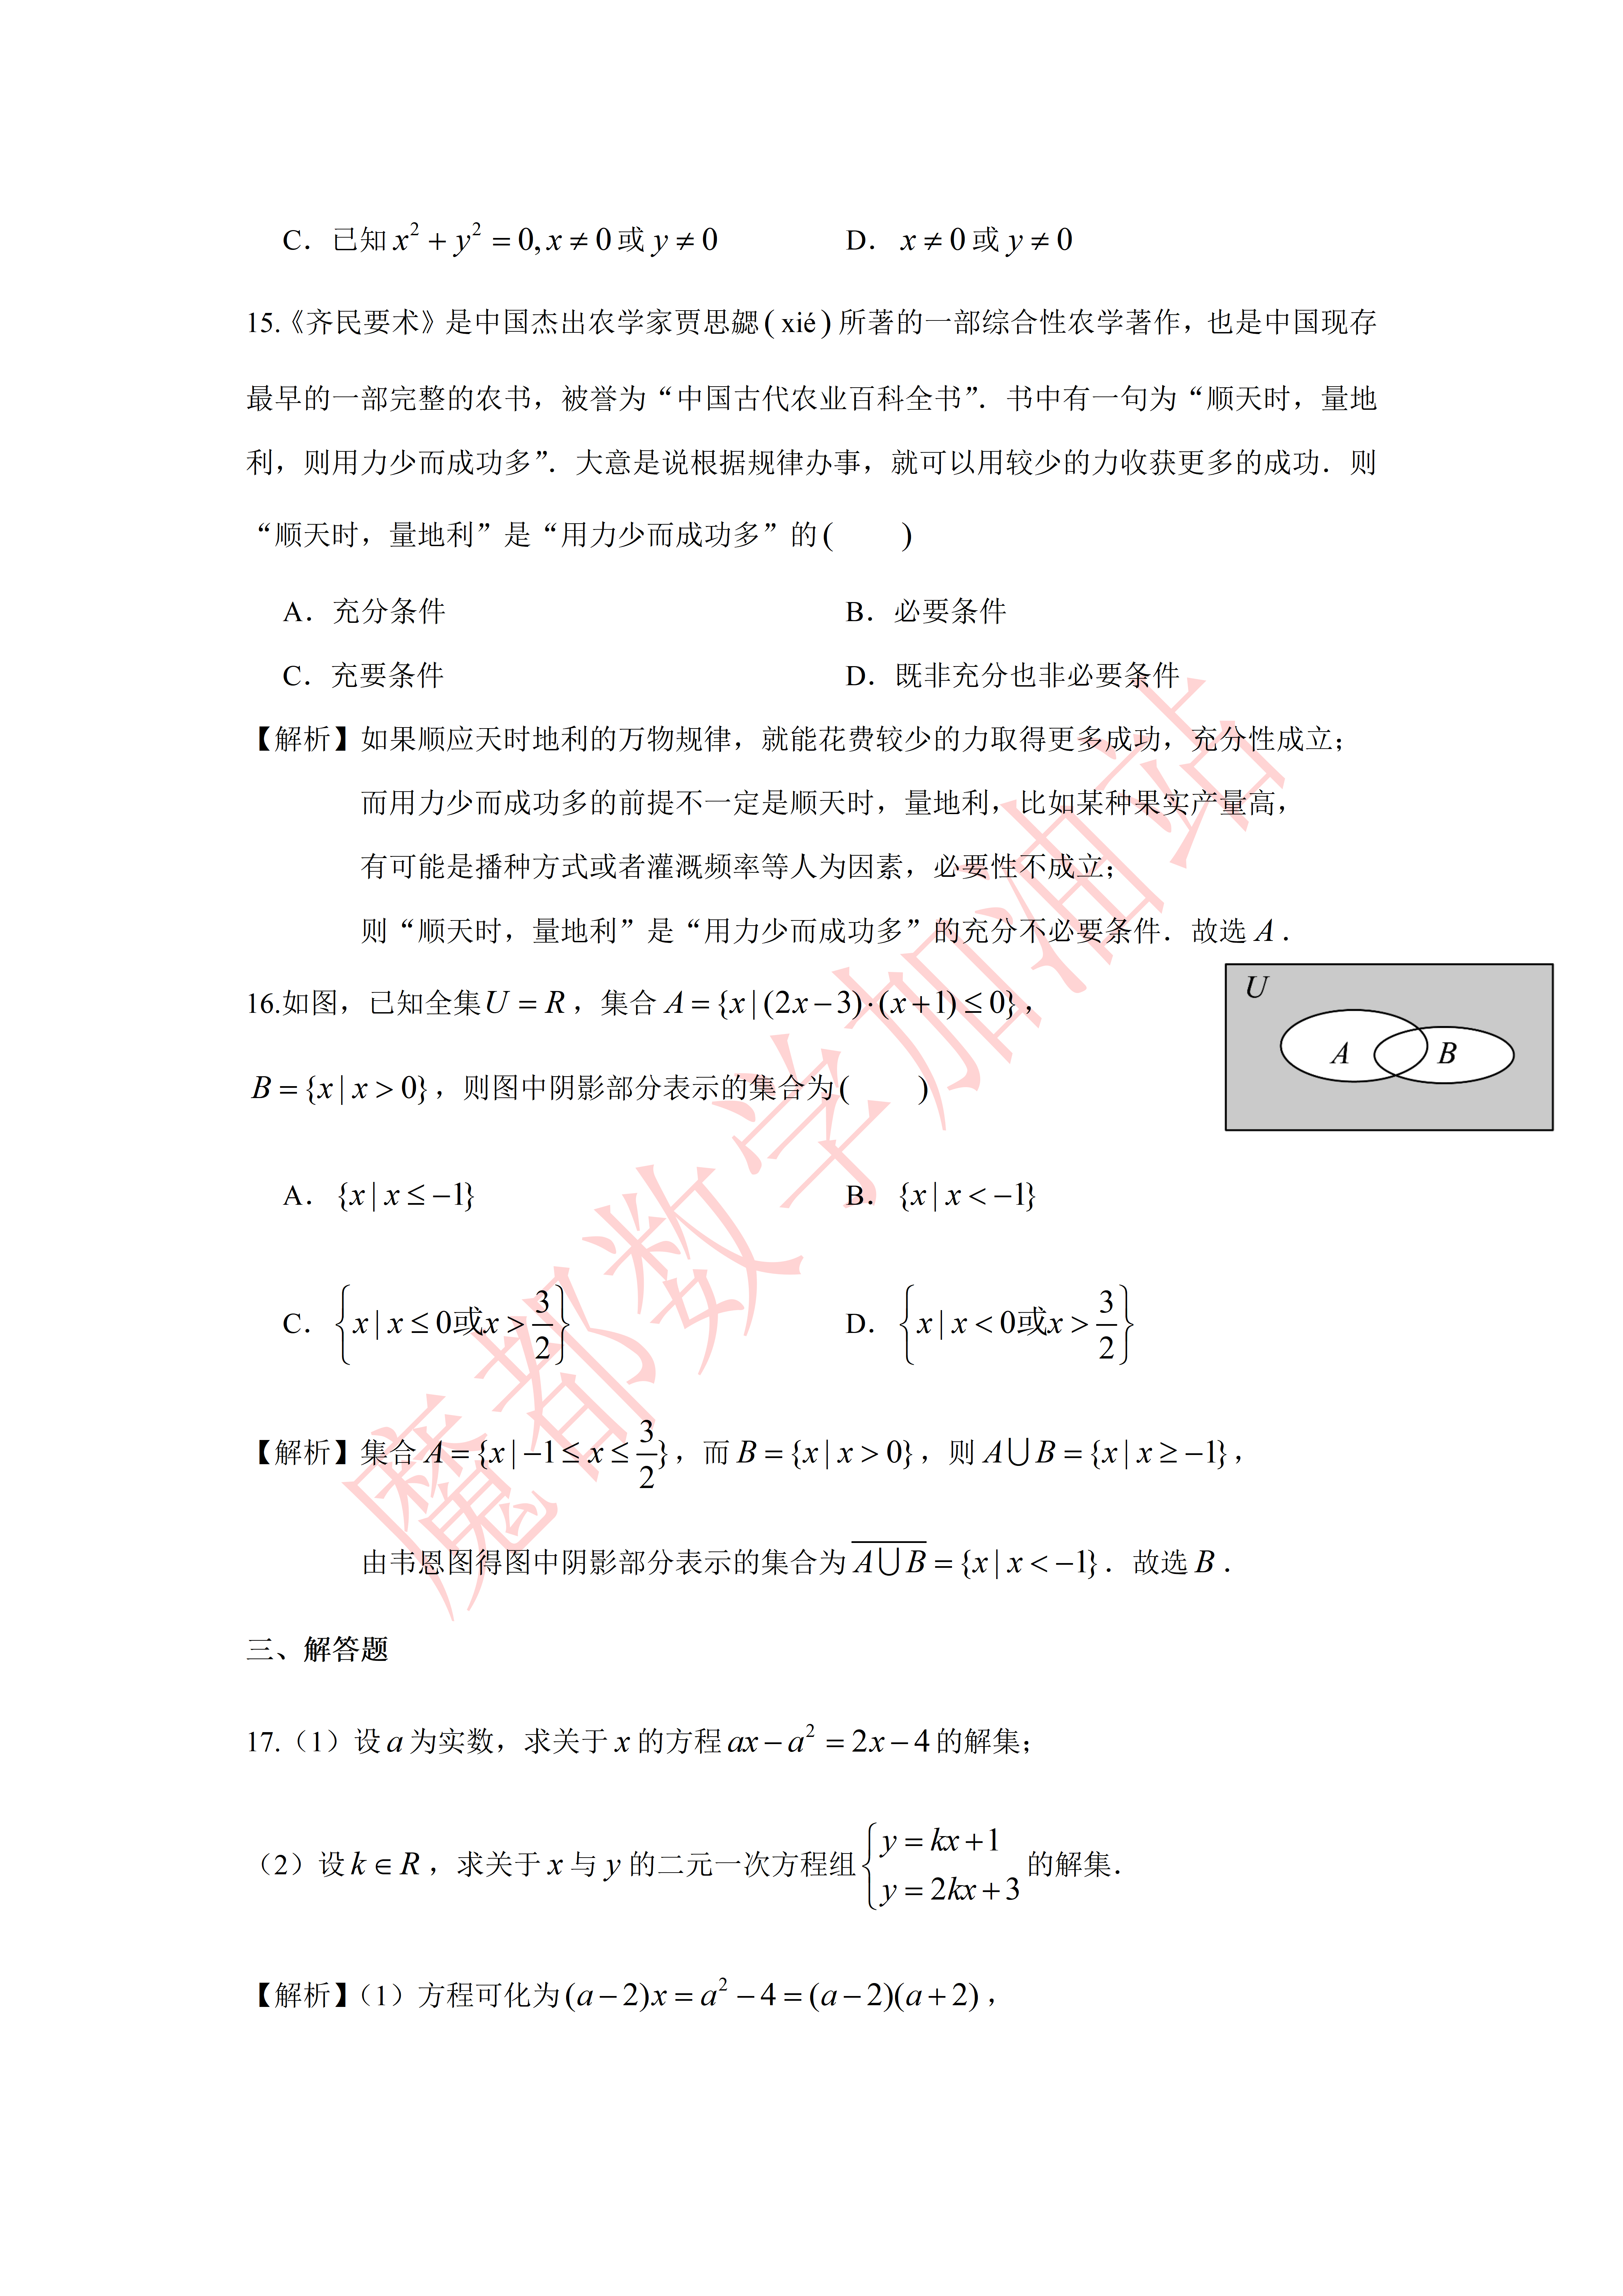
\includegraphics[width=.34\linewidth,trim=3586bp 3410bp 196bp 2818bp,clip]{../原图/高一52_回民中学_9月月考/04.png}
\end{center}

\keepwithprev
A. $\{x\mid x\leqslant-1\}$\qquad B. $\{x\mid x<-1\}$

C. $\left\{x\mid x\leqslant0\text{ 或 }x>\dfrac32\right\}$\qquad D. $\left\{x\mid x<0\text{ 或 }x>\dfrac32\right\}$

\ifanswer
\solbegin
\step{集合 $A=\left\{x\mid-1\leqslant x\leqslant\dfrac32\right\}$，而 $B=\{x\mid x>0\}$，则 $A\cup B=\{x\mid x\geqslant-1\}$，}
\step{由韦恩图得图中阴影部分表示的集合为 $\overline{A\cup B}=\{x\mid x<-1\}$．故选 $B$．}
\solend
\fi

\end{enumerate}

\bigsec{三、解答题}

\begin{enumerate}
\setcounter{enumi}{16}

\item （1）设 $a$ 为实数，求关于 $x$ 的方程 $ax-a^2=2x-4$ 的解集；

（2）设 $k\in\R$，求关于 $x$ 与 $y$ 的二元一次方程组 $\begin{cases}y=kx+1\\y=2kx+3\end{cases}$ 的解集．

\ifanswer
\solbegin
\stepm{(1)}{方程可化为 $(a-2)x=a^2-4=(a-2)(a+2)$，}
\step{当 $a\neq2$ 时，方程的解为 $x=\dfrac{(a-2)(a+2)}{a-2}=a+2$，则解集为 $\{a+2\}$；}
\step{当 $a=2$ 时，方程为 $2x-4=2x-4$，对 $x$ 取一切实数均成立，}
\step{所以解集为 $\R$；}
\stepm{(2)}{$\begin{cases}y=kx+1\\y=2kx+3\end{cases}$，则 $kx+1=2kx+3,kx=-2$，}
\step{当 $k=0$ 时，等式不成立，无解；当 $k\neq0$ 时，$x=-\dfrac2k,y=-1$；}
\step{综上所述，当 $k=0$ 时，解集为 $\varnothing$；当 $k\neq0$ 时，解集为 $\left\{\left(-\dfrac2k,-1\right)\right\}$．}
\solend
\fi

\ansspace[6]

\item 已知命题 $p$：方程 $x^2+6x+m-1=0$ 有两个不等的负根；命题 $q$：方程 $9x^2+6x+m-2=0$ 无实根．

\begin{enumerate}[label=(\arabic*)]
\item 若 $p$ 为真命题，求实数 $m$ 的取值范围；
\item 若 $p,q$ 两命题一真一假，求实数 $m$ 的取值范围．
\end{enumerate}

\ifanswer
\solbegin
\stepm{(1)}{设方程 $x^2+6x+m-1=0$ 两根为 $x_1,x_2$，}
\step{则 $\begin{cases}\Delta>0\\ x_1+x_2<0\\ x_1x_2>0\end{cases}\Rightarrow\begin{cases}36-4(m-1)>0\\ -6<0\\ m-1>0\end{cases}\Rightarrow1<m<10$；}
\stepm{(2)}{若命题 $q$ 为真命题，则 $36-36(m-2)<0\Rightarrow m>3$，}
\step{从而当命题 $q$ 为假命题时，$m\leqslant3$；}
\step{又由（1）得 $p$ 为假命题时，$m\leqslant1$ 或 $m\geqslant10$；}
\step{则当 $p$ 为真命题，$q$ 为假命题时，得 $\begin{cases}1<m<10\\ m\leqslant3\end{cases}\Rightarrow1<m\leqslant3$；}
\step{当 $q$ 为真命题，$p$ 为假命题时，得 $\begin{cases}m\leqslant1\text{ 或 }m\geqslant10\\ m>3\end{cases}\Rightarrow m\geqslant10$；}
\step{综上，当 $p,q$ 两命题一真一假时，$1<m\leqslant3$ 或 $m\geqslant10$.}
\solend
\fi

\ansspace[6]

\item 证明下列两个命题：

\begin{enumerate}[label=(\arabic*)]
\item 设 $ab>0$，求证：$a>b$ 是 $\dfrac1a<\dfrac1b$ 的充要条件．
\item 已知 $a,b$ 为正数，$n$ 为正整数，求证：如果 $a^n>b^n$，那么 $a>b$．
\end{enumerate}

\ifanswer
\solbegin
\stepm{(1)}{先证充分性：因为 $ab>0$ 且 $a>b$，故 $a-b>0$，从而 $\dfrac{a-b}{ab}>0$，}
\step{即 $\dfrac1b-\dfrac1a>0$，即 $\dfrac1a<\dfrac1b$；}
\step{再证必要性：若 $\dfrac1a<\dfrac1b$，则 $\dfrac1a-\dfrac1b=\dfrac{b-a}{ab}<0$，}
\step{又因为 $ab>0$，所以 $b-a<0$，即 $a>b$．}
% 原卷如此，照录未改（第 19 题(1)此句末用全角句号“。”，全卷其余各题末句用“．”，
% 见文件头“原卷笔误/存疑”第 4 条）
\step{综上，$a>b$ 是 $\dfrac1a<\dfrac1b$ 的充要条件。}
\stepm{(2)}{令 $f(x)=x^n,n\in\N^*$，则由幂函数的性质得 $f(x)$ 在第一象限是严格增的，}
\step{而 $a^n>b^n$ 即意味着 $f(a)>f(b)$，且 $a,b$ 为正数，从而 $a>b$．}
\solend
\fi

\ansspace[8]

\item （1）求关于 $x$ 的不等式 $(m-2)x>1-m$ 的解集；

（2）求关于 $x$ 的不等式 $x^2-(a+1)x+a\leqslant0$ 的解集．

\ifanswer
\solbegin
\stepm{(1)}{由不等式 $(m-2)x>1-m$，}
\step{当 $m-2>0$ 时，即 $m>2$ 时，解得 $x>\dfrac{1-m}{m-2}$，}
\step{所以不等式的解集为 $\left(\dfrac{1-m}{m-2},+\infty\right)$；}
\step{当 $m-2=0$ 时，即 $m=2$ 时，不等式即为 $0>-1$ 恒成立，}
\step{即不等式的解集为 $\R$；}
\step{当 $m-2<0$ 时，即 $m<2$ 时，解得 $x<\dfrac{1-m}{m-2}$，}
\step{所以不等式的解集为 $\left(-\infty,\dfrac{1-m}{m-2}\right)$；}
\step{综上，当 $m>2$ 时，解集为 $\left(\dfrac{1-m}{m-2},+\infty\right)$；}
\step{当 $m=2$ 时，解集为 $\R$；}
\step{当 $m<2$ 时，解集为 $\left(-\infty,\dfrac{1-m}{m-2}\right)$．}
\stepm{(2)}{由不等式 $x^2-(a+1)x+a\leqslant0$，可化为 $(x-a)(x-1)\leqslant0$，}
\step{当 $a>1$ 时，解得 $1\leqslant x\leqslant a$，即不等式的解集为 $[1,a]$；}
\step{当 $a=1$ 时，不等式即为 $(x-1)^2\leqslant0$，解得 $x=1$，即不等式的解集为 $\{1\}$；}
\step{当 $a<1$ 时，解得 $a\leqslant x\leqslant1$，即不等式的解集为 $[a,1]$，}
\step{综上，当 $a>1$ 时，解集为 $[1,a]$；}
\step{当 $a=1$ 时，解集为 $\{1\}$；}
\step{当 $a<1$ 时，解集为 $[a,1]$．}
\solend
\fi

\ansspace[10]

\item 已知集合 $A=\{x\mid(x+2)(5-x)\geqslant0\}$，若集合 $B$ 满足 $A\cap B=\varnothing,A\cup B=[-2,7)$．

\begin{enumerate}[label=(\arabic*)]
\item 用区间表示集合 $B$；
\item 若集合 $B$ 是不等式 $-x^2+bx+c>0$ 的解集，求实数 $b,c$ 的值；
\item 已知全集为 $\R$，若关于 $x$ 的不等式 $-1<x-a\leqslant2$ 的解集为 $M$，且“$x\in\overline A$”是“$x\in M$”的必要非充分条件，求实数 $a$ 的取值范围．
\end{enumerate}

\ifanswer
\solbegin
\stepm{(1)}{由题意得 $(x+2)(5-x)\geqslant0\Leftrightarrow(x+2)(x-5)\leqslant0\Rightarrow-2\leqslant x\leqslant5$，}
\step{则 $A=[-2,5]$，又 $A\cap B=\varnothing,A\cup B=[-2,7)$，则 $B=(5,7)$；}
\stepm{(2)}{$-x^2+bx+c>0\Leftrightarrow x^2-bx-c<0$，则 $x^2-bx-c=0$ 两根为 $5,7$，}
\step{则由韦达定理得 $b=12,-c=35\Rightarrow c=-35$；}
\stepm{(3)}{由题意得 $M=(a-1,a+2],\overline A=(-\infty,-2)\cup(5,+\infty)$，}
\step{且“$x\in\overline A$”是“$x\in M$”的必要非充分条件，则 $M$ 是 $\overline A$ 的真子集，}
\step{从而 $a+2<-2$ 或 $a-1\geqslant5$，解得 $a<-4$ 或 $a\geqslant6$，}
\step{所以实数 $a$ 的取值范围为 $(-\infty,-4)\cup[6,+\infty)$．}
\solend
\fi

\ansspace*[10]

\end{enumerate}

\end{document}
"
% 紧凑版：xelatex "\def\iscompact{1}% 高一52_回民中学_9月月考.tex
%   —— 高一上数学“2026-2027 年回民中学高一上 9 月月考”（讲评版）
% 试卷版：xelatex 高一52_回民中学_9月月考.tex
% 答案版：xelatex "\def\isanswer{1}% 高一52_回民中学_9月月考.tex
%   —— 高一上数学“2026-2027 年回民中学高一上 9 月月考”（讲评版）
% 试卷版：xelatex 高一52_回民中学_9月月考.tex
% 答案版：xelatex "\def\isanswer{1}\input{高一52_回民中学_9月月考.tex}"
% 紧凑版：xelatex "\def\iscompact{1}\input{高一52_回民中学_9月月考.tex}"
%
% 原始材料：微信公众号“魔都数学加油站”文章，作者破晓，连载“27学年高一52”；
% 原文标题“27学年高一52——2026-2027年上海市回民中学高一上9月月考”；
% 原文链接：https://mp.weixin.qq.com/s/ndjyozrRQCLl4ba3J8uR7g。
% 该页面用 JS 渲染，未见明确发布日期；页面内时间戳约为 2026-10-06 21:19／21:38，本稿以该时刻记可得日期。
% 正文为 8 张 PNG 页：第 01—07 页 4762×6735，第 08 页 2560×3620（**同一篇各页分辨率不同**），
% 均按页序读取。8 页全为试卷正文页（卷首标题在第 1 页页顶，卷末解答题第 21 题解析止于第 8 页），
% 无封面页、目录页、二维码或宣传页。粉色斜排“魔都数学加油站”为卷面水印，与公众号页脚一并未录入。
%
% 卷首标题：照卷面印作“2026--2027 年回民中学高一上 9 月月考”（公众号标题中的“上海市”
% 卷面标题行没有，本稿照卷面），年份区间按全稿惯例排 en dash。原卷只有一行标题、无副标题。
%
% 篇幅与题号：原卷自第 3 题起编号（第 1、2 题不在本卷内）。填空题 3—12（10 题）、
% 选择题 13—16（4 题）、解答题 17—21（5 题），共 19 题。本稿沿用原节与原题号，
% 只改排为全稿统一的大节样式（原卷小节标题为“一、填空题”“二、选择题”“三、解答题”）。
%
% 讲评版：原卷每题下直接印【答案】或【解析】。**只印【答案】的 1 题**（第 3 题），本稿只给 \ans{}；
% **第 14 题没有任何【答案】/【解析】段**，答案“D”直接印在题干括号内（“应假设(  D  )”），
% 本稿按 高一37 第 13 题的成例把括号留空、答案另提为 \ans{$D$}；
% 其余 17 题都只印【解析】，按全稿口径这类题不另提 \ans{}——其中选择题第 13、15、16 题的结论
% 写在解析末句（“故选 A／A／B”），亦照录在解析内。
%
% 副标题：原卷未印副标题。本稿按“知识模块”口径标作“集合与常用逻辑用语、不等式”：
% 19 题中集合与常用逻辑用语 10 题（集合类 7 题——第 3、4、5、9、12、16、21 题；
% 逻辑类 3 题——第 6、14、15 题），不等式 9 题（含等式性质与一元二次方程：第 7、8、10、11、
% 13、17、18、19、20 题），两类均远超三分之一，故并标。口径同 高一46、高一47、高一48、高一51。
%
% 与原卷的排版差异：
%   ① 原卷每题下直接印【答案】/【解析】，本稿按全稿惯例将答案与解析置于答案版，试卷版保持干净；
%      第 14 题印在题干括号内的答案“D”同样移入 \ans{}，见上；
%   ② 原卷未印副标题，本稿按“知识模块”口径补出；
%   ③ 原卷填空横线约两个字宽，本稿按全稿惯例统一排 \blankline[4.4em]；
%      选择题的作答括号原卷排半角“(    )”，本稿按全稿惯例排 \mbox{（\quad）}；
%   ④ 原卷实数集、自然数集排斜体/粗体 $R$、$\mathbf{R}$、$N$，本稿按全稿惯例改用 $\R$、$\N$；
%      空集记号统一为 \varnothing；
%   ⑤ 第 8 题题干与解析两处“两个实数分别为 $x_1$、$x_2$”原卷即用顿号，第 10、13 题等处
%      原卷在数学式内用半角逗号（如 $x_1,x_2$、$a,b,c\in R$），两份均照录未强改；
%      句末句点按全稿惯例排西文句点，句中句点（第 9、12、15、21 题）照原卷排全角“．”；
%   ⑥ 第 17、20 题原卷把子问标号“（1）”排在该题题号同一行，本稿照原卷仍排同一行（同 高一34 的
%      做法）；第 18、19、21 题的子问原卷各自另起一行，本稿按全稿惯例用 enumerate 的 (1)(2)(3)；
%      解析中的子问标号一律用 \stepm{(1)}{…}；
%   ⑦ 第 16 题的韦恩图原卷排在题干与选项右侧的浮动位置，本稿居中排在题干之后、选项之前，
%      并加 \needvspace 整块推走（守卫写在 \item 之前）；图自原图第 4 页裁切（trim），不另存图片文件；
%   ⑧ 每道解答题原卷未留作答空白，本稿按全稿惯例加 \ansspace。
%
% 原卷笔误/存疑（均照录未改，正文对应处另有 % 注）：
%   1. 第 8 题题干与解析首行两处均作“两个实数分别为 $x_1$、$x_2$”，按文意应为“两个实数**根**”
%      （疑脱“根”字，第 10 题同位置作“两个实根分别是”）；
%   2. 第 4 题解析“满足条件的 $A$ 的个数为集合 $\{0,1,3\}$ 的真子集，即 7 个”，
%      “个数为……真子集”表述不严（应为“……的真子集的个数”）；$\{0,1,3\}$ 的真子集 7 个，结论无误；
%   3. 第 6 题解析第 2 行“当 $a=10,b=0.2$ 时，$a+b>2$，且 $ab>1$，所以 $a>1$，且 $b>1$ 不成立”
%      ——此处是举反例，“所以”按文意应为“但”（$a=10,b=0.2$ 与“$a>1$ 且 $b>1$”不成立之间是转折，
%      非因果）；
%   4. 第 19 题 (1) 解析末行“综上，$a>b$ 是 $\dfrac1a<\dfrac1b$ 的充要条件。”用全角句号“。”，
%      全卷其余各题末句均用“．”，体例不一，照录；
%   5. 第 20 题第 (1) 问解析先按 $m>2$、$m=2$、$m<2$ 三种情况各给出解集，末三行又“综上”重述一遍，
%      与原卷一致（内容重复，非笔误）；
%   6. 第 18 题题干第 (2) 问“若 $p,q$ 两命题一真一假”，正文照录原卷所用半角逗号（未改顿号）。
%
% 插图：1 张，自原图裁切（无 \begin{tikzpicture} 重排）：
%   · 第 16 题题干韦恩图（全集 $U$ 矩形内两相交椭圆 $A$、$B$，灰色为阴影部分）
%     ——原图第 04 页，原卷排于题干与选项右侧。
%     裁框：x 3594–4558、y 2826–3317（即矩形外框，四周各留 4px），
%     trim=3590bp 3414bp 200bp 2822bp（左／下／右／上），页宽 4762、页高 6735。
%
\documentclass[a4paper,11pt]{article}
\usepackage{common}

\begin{document}

\examtitlest[3]{2026--2027 年回民中学高一上 9 月月考}{集合与常用逻辑用语、不等式}

\bigsec{一、填空题}

\begin{enumerate}
\setcounter{enumi}{2}

\item 用列举法写出下列集合 $\{(x,y)\mid x+y=2,x\in\N,y\in\N\}=$\blankline[4.4em].

\ifanswer
\ans{$\{(0,2),(1,1),(2,0)\}$}
\fi

\item 设集合 $A$ 满足 $\{-1,2\}\sub A\subset\{-1,0,1,2,3\}$，则满足条件的 $A$ 有\blankline[4.4em]个.

\ifanswer
\solbegin
\step{满足条件的 $A$ 的个数为集合 $\{0,1,3\}$ 的真子集，即 $7$ 个.}
\solend
\fi

\item 已知集合 $A=\{2,(a+1)^2,a^2+2\}$，且 $1\in A$，则实数 $a$ 的值为\blankline[4.4em].

\ifanswer
\solbegin
\step{因为 $1\in A$，而 $a^2+2\geqslant2$，所以 $(a+1)^2=1$，解得 $a=0$ 或 $a=-2$，}
\step{$a=0$ 时，$a^2+2=2$，不合题意，$a=-2$ 时，$a^2+2=6$，满足题意，}
\step{所以 $a=-2$.}
\solend
\fi

\item 已知 $a,b$ 是实数，则“$a>1$，且 $b>1$”是“$a+b>2$，且 $ab>1$”的\blankline[4.4em]条件.

\ifanswer
\solbegin
\step{$a,b$ 是实数，则“$a>1$，且 $b>1$”$\Rightarrow$“$a+b>2$，且 $ab>1$”正确，}
% 原卷如此，照录未改（第 6 题解析此处作“所以 $a>1$，且 $b>1$ 不成立”，按文意为转折，
% 见文件头“原卷笔误/存疑”第 3 条）
\step{当 $a=10,b=0.2$ 时，$a+b>2$，且 $ab>1$，所以 $a>1$，且 $b>1$ 不成立，}
\step{即前者是推出后者，后者推不出前者，}
\step{所以“$a>1$，且 $b>1$”是“$a+b>2$，且 $ab>1$”的充分而不必要条件.}
\solend
\fi

\item 已知等式 $2x^2-3x-1=a(x-1)^2+b(x-1)+c$ 恒成立，其中 $a,b,c$ 为常数，则 $a+b-c=$\blankline[4.4em].

\ifanswer
\solbegin
\step{将等式右侧展开整理得 $a(x-1)^2+b(x-1)+c=ax^2+(-2a+b)x+(a-b+c)$，}
\step{左右两边多项式恒等，对应次数的系数必须相等：}
\step{则 $a=2,-2a+b=-3$，代入 $a=2$ 得 $b=1$，$a-b+c=-1$，}
\step{代入 $a=2,b=1$ 得 $c=-2$，得 $a+b-c=2+1-(-2)=5$.}
\solend
\fi

% 原卷如此，照录未改（第 8 题题干与解析首行两处“两个实数分别为”疑脱“根”字，
% 见文件头“原卷笔误/存疑”第 1 条）
\item 若关于 $x$ 的二次方程 $x^2+mx+4m^2-3=0$ 的两个实数分别为 $x_1$、$x_2$，且满足 $x_1+x_2=x_1x_2$，则实数 $m$ 的值为\blankline[4.4em].

\ifanswer
\solbegin
% 原卷如此，照录未改（此处“两个实数分别为”同题干，疑脱“根”字）
\step{二次方程 $x^2+mx+4m^2-3=0$ 的两个实数分别为 $x_1$、$x_2$，}
\step{则有 $\Delta=m^2-4(4m^2-3)\geqslant0$，变形得 $m^2\leqslant\dfrac45$，}
\step{则 $x_1+x_2=-m$，$x_1x_2=(4m^2-3)$，}
\step{若 $x_1+x_2=x_1x_2$，则有 $-m=4m^2-3$，解得 $m=-1$ 或 $\dfrac34$，}
\step{又 $m^2\leqslant\dfrac45$，则 $m=\dfrac34$.}
\solend
\fi

\item 设集合 $A=\{x\mid x^2=1\}$，$B=\{x\mid ax=1\}$．若 $A\cap B=B$，则实数 $a$ 的值为\blankline[4.4em].

\ifanswer
\solbegin
\step{集合 $A=\{x\mid x^2=1\}=\{-1,1\}$，$B=\{x\mid ax=1\}$，$A\cap B=B$，所以 $B\sub A$，}
\step{当 $a=0$ 时，$B=\varnothing$，成立；}
\step{当 $a\neq0$ 时，$B=\left\{\dfrac1a\right\}$，则 $\dfrac1a=-1$ 或 $\dfrac1a=1$，解得 $a=-1$ 或 $a=1$，}
\step{所以实数 $a$ 的值为 $0$ 或 $1$ 或 $-1$.}
\solend
\fi

\item 已知关于 $x$ 的一元二次方程 $x^2+3x-3=0$ 的两个实根分别是 $x_1,x_2$，则以 $-\dfrac1{x_1},-\dfrac1{x_2}$ 为根且二次项系数是 $1$ 的一元二次方程为\blankline[4.4em].

\ifanswer
\solbegin
\step{因为 $x_1,x_2$ 是一元二次方程 $x^2+3x-3=0$ 的两个实根，}
\step{所以 $x_1+x_2=-3,x_1x_2=-3$，}
\step{所以 $-\dfrac1{x_1}+\left(-\dfrac1{x_2}\right)=-\dfrac{x_1+x_2}{x_1x_2}=-1$，$-\dfrac1{x_1}\cdot\left(-\dfrac1{x_2}\right)=\dfrac1{x_1x_2}=-\dfrac13$，}
\step{所以一元二次方程为 $x^2+x-\dfrac13=0$.}
\solend
\fi

\item 若关于 $x$ 的不等式 $(a-2)x^2+2(a-2)x-4<0$ 的解集是 $\R$，则实数 $a$ 的取值范围是\blankline[4.4em].

\ifanswer
\solbegin
\step{当 $a=2$ 时，不等式化为 $-4<0$ 对于任意实数 $x$ 都成立，因此 $a=2$ 满足题意；}
\step{当 $a\neq2$ 时，要使关于 $x$ 的不等式 $(a-2)x^2+2(a-2)x-4<0$ 的解集为 $\R$，}
\step{则 $\begin{cases}a-2<0\\ \Delta=4(a-2)^2+16(a-2)<0\end{cases}$，解得 $-2<a<2$．}
\step{综上，$a$ 的取值范围为 $(-2,2]$．}
\solend
\fi

\item 设非空集合 $A$、$B$，定义 $A\times B=\{x\mid x\in(A\cup B),x\notin(A\cap B)\}$．已知 $A=\{x\mid0\leqslant x\leqslant2\}$，$B=\{y\mid y\geqslant0\}$，则 $A\times B=$\blankline[4.4em].

\ifanswer
\solbegin
\step{由于 $A=\{x\mid0\leqslant x\leqslant2\}$，$B=\{y\mid y\geqslant0\}=\{x\mid x\geqslant0\}$，}
\step{所以 $A\cup B=\{x\mid x\geqslant0\}$，$A\cap B=\{x\mid0\leqslant x\leqslant2\}$，故 $A\times B=\{x\mid x>2\}$．}
\solend
\fi

\end{enumerate}

\bigsec{二、选择题}

\begin{enumerate}
\setcounter{enumi}{12}

\item 已知 $a,b,c\in\R$ 且 $a>b$，则下列不等式一定成立的是\mbox{（\quad）}

\keepwithprev
A. $\dfrac{a}{c^2+1}>\dfrac{b}{c^2+1}$\qquad B. $\dfrac1a<\dfrac1b$

C. $ac>bc$\qquad D. $a^2>b^2$

\ifanswer
\solbegin
\step{对于 A：因为 $c^2+1>0$ 恒成立，且 $a>b$，所以 $\dfrac{a}{c^2+1}>\dfrac{b}{c^2+1}$ 一定成立，}
\step{所以 A 正确；}
\step{对于 B：当 $a=1,b=-1$ 时，满足 $a>b$，此时 $\dfrac1a=1>\dfrac1b=-1$，所以 B 错误；}
\step{对于 C：当 $c<0$ 时，由 $a>b$，得 $ac<bc$，所以 C 错误；}
\step{对于 D：当 $a=1,b=-2$ 时，满足 $a>b$，此时 $a^2=1<b^2=4$，所以 D 错误；}
\step{故选 $A$．}
\solend
\fi

% 注：本题的答案“D”原卷直接印在题干末尾的括号内（“应假设(  D  )”），且没有单独的
%     【答案】/【解析】段，本稿按 高一37 第 13 题的成例把括号留空、另提为 \ans{}，
%     见文件头“与原卷的排版差异”①。
\item 用反证法证明：“已知 $x,y\in\R$,$x^2+y^2=0$，求证：$x=y=0$”时，应假设\mbox{（\quad）}

\keepwithprev
A. 已知 $x^2+y^2=0,x\neq0$ 且 $y\neq0$\qquad B. $x\neq0$ 且 $y\neq0$

C. 已知 $x^2+y^2=0,x\neq0$ 或 $y\neq0$\qquad D. $x\neq0$ 或 $y\neq0$

\ans{$D$}

\item 《齐民要术》是中国杰出农学家贾思勰（xié）所著的一部综合性农学著作，也是中国现存最早的一部完整的农书，被誉为“中国古代农业百科全书”．书中有一句为“顺天时，量地利，则用力少而成功多”．大意是说根据规律办事，就可以用较少的力收获更多的成功．则“顺天时，量地利”是“用力少而成功多”的\mbox{（\quad）}

\keepwithprev
A. 充分条件\qquad B. 必要条件

C. 充要条件\qquad D. 既非充分也非必要条件

\ifanswer
\solbegin
\step{如果顺应天时地利的万物规律，就能花费较少的力取得更多成功，充分性成立；}
\step{而用力少而成功多的前提不一定是顺天时，量地利，比如某种果实产量高，}
\step{有可能是播种方式或者灌溉频率等人为因素，必要性不成立；}
\step{则“顺天时，量地利”是“用力少而成功多”的充分不必要条件．故选 $A$．}
\solend
\fi

\needvspace{13\baselineskip}

\item 如图，已知全集 $U=\R$，集合 $A=\{x\mid(2x-3)\cdot(x+1)\leqslant0\}$，$B=\{x\mid x>0\}$，则图中阴影部分表示的集合为\mbox{（\quad）}

\begin{center}
% 原图第 4 页题干韦恩图直接裁取（原卷排于题干与选项右侧）。
% 裁框取矩形外框 x 3590–4558、y 2822–3321，再向外各留 4px（即 x 3586–4562、y 2818–3325），
% trim=左 3586bp／下 3410bp／右 196bp／上 2818bp（页宽 4762、页高 6735）。
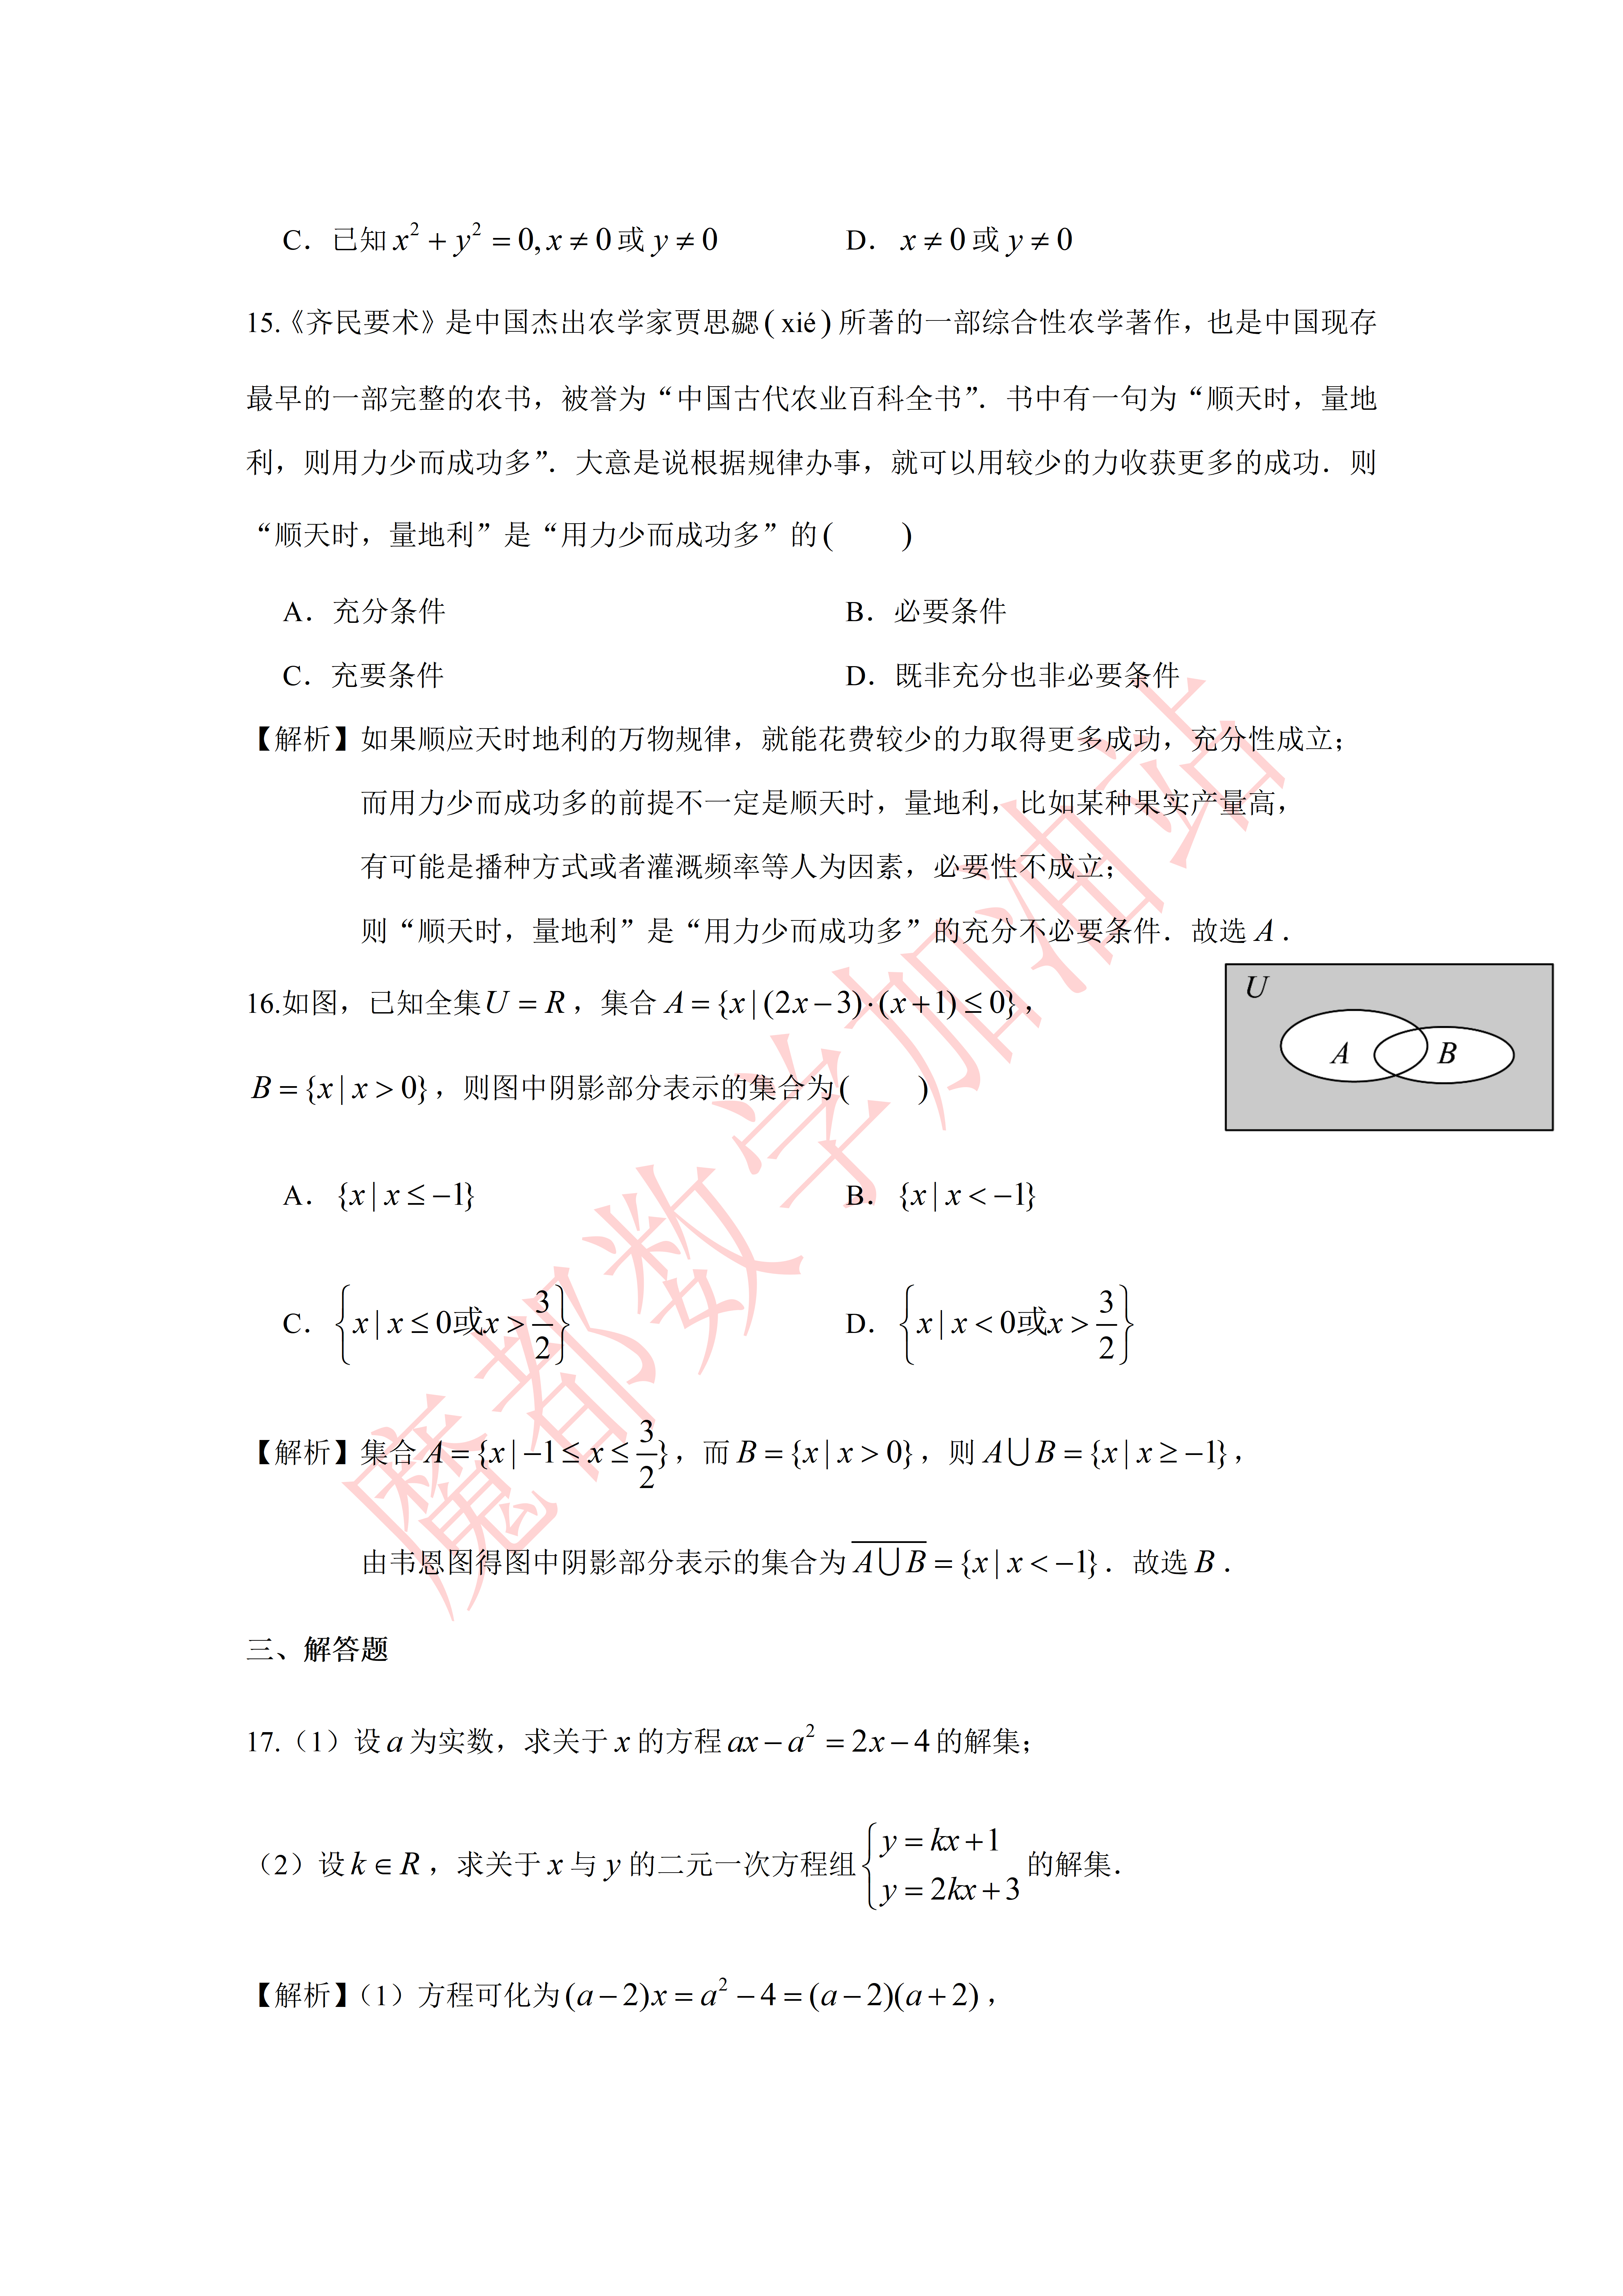
\includegraphics[width=.34\linewidth,trim=3586bp 3410bp 196bp 2818bp,clip]{../原图/高一52_回民中学_9月月考/04.png}
\end{center}

\keepwithprev
A. $\{x\mid x\leqslant-1\}$\qquad B. $\{x\mid x<-1\}$

C. $\left\{x\mid x\leqslant0\text{ 或 }x>\dfrac32\right\}$\qquad D. $\left\{x\mid x<0\text{ 或 }x>\dfrac32\right\}$

\ifanswer
\solbegin
\step{集合 $A=\left\{x\mid-1\leqslant x\leqslant\dfrac32\right\}$，而 $B=\{x\mid x>0\}$，则 $A\cup B=\{x\mid x\geqslant-1\}$，}
\step{由韦恩图得图中阴影部分表示的集合为 $\overline{A\cup B}=\{x\mid x<-1\}$．故选 $B$．}
\solend
\fi

\end{enumerate}

\bigsec{三、解答题}

\begin{enumerate}
\setcounter{enumi}{16}

\item （1）设 $a$ 为实数，求关于 $x$ 的方程 $ax-a^2=2x-4$ 的解集；

（2）设 $k\in\R$，求关于 $x$ 与 $y$ 的二元一次方程组 $\begin{cases}y=kx+1\\y=2kx+3\end{cases}$ 的解集．

\ifanswer
\solbegin
\stepm{(1)}{方程可化为 $(a-2)x=a^2-4=(a-2)(a+2)$，}
\step{当 $a\neq2$ 时，方程的解为 $x=\dfrac{(a-2)(a+2)}{a-2}=a+2$，则解集为 $\{a+2\}$；}
\step{当 $a=2$ 时，方程为 $2x-4=2x-4$，对 $x$ 取一切实数均成立，}
\step{所以解集为 $\R$；}
\stepm{(2)}{$\begin{cases}y=kx+1\\y=2kx+3\end{cases}$，则 $kx+1=2kx+3,kx=-2$，}
\step{当 $k=0$ 时，等式不成立，无解；当 $k\neq0$ 时，$x=-\dfrac2k,y=-1$；}
\step{综上所述，当 $k=0$ 时，解集为 $\varnothing$；当 $k\neq0$ 时，解集为 $\left\{\left(-\dfrac2k,-1\right)\right\}$．}
\solend
\fi

\ansspace[6]

\item 已知命题 $p$：方程 $x^2+6x+m-1=0$ 有两个不等的负根；命题 $q$：方程 $9x^2+6x+m-2=0$ 无实根．

\begin{enumerate}[label=(\arabic*)]
\item 若 $p$ 为真命题，求实数 $m$ 的取值范围；
\item 若 $p,q$ 两命题一真一假，求实数 $m$ 的取值范围．
\end{enumerate}

\ifanswer
\solbegin
\stepm{(1)}{设方程 $x^2+6x+m-1=0$ 两根为 $x_1,x_2$，}
\step{则 $\begin{cases}\Delta>0\\ x_1+x_2<0\\ x_1x_2>0\end{cases}\Rightarrow\begin{cases}36-4(m-1)>0\\ -6<0\\ m-1>0\end{cases}\Rightarrow1<m<10$；}
\stepm{(2)}{若命题 $q$ 为真命题，则 $36-36(m-2)<0\Rightarrow m>3$，}
\step{从而当命题 $q$ 为假命题时，$m\leqslant3$；}
\step{又由（1）得 $p$ 为假命题时，$m\leqslant1$ 或 $m\geqslant10$；}
\step{则当 $p$ 为真命题，$q$ 为假命题时，得 $\begin{cases}1<m<10\\ m\leqslant3\end{cases}\Rightarrow1<m\leqslant3$；}
\step{当 $q$ 为真命题，$p$ 为假命题时，得 $\begin{cases}m\leqslant1\text{ 或 }m\geqslant10\\ m>3\end{cases}\Rightarrow m\geqslant10$；}
\step{综上，当 $p,q$ 两命题一真一假时，$1<m\leqslant3$ 或 $m\geqslant10$.}
\solend
\fi

\ansspace[6]

\item 证明下列两个命题：

\begin{enumerate}[label=(\arabic*)]
\item 设 $ab>0$，求证：$a>b$ 是 $\dfrac1a<\dfrac1b$ 的充要条件．
\item 已知 $a,b$ 为正数，$n$ 为正整数，求证：如果 $a^n>b^n$，那么 $a>b$．
\end{enumerate}

\ifanswer
\solbegin
\stepm{(1)}{先证充分性：因为 $ab>0$ 且 $a>b$，故 $a-b>0$，从而 $\dfrac{a-b}{ab}>0$，}
\step{即 $\dfrac1b-\dfrac1a>0$，即 $\dfrac1a<\dfrac1b$；}
\step{再证必要性：若 $\dfrac1a<\dfrac1b$，则 $\dfrac1a-\dfrac1b=\dfrac{b-a}{ab}<0$，}
\step{又因为 $ab>0$，所以 $b-a<0$，即 $a>b$．}
% 原卷如此，照录未改（第 19 题(1)此句末用全角句号“。”，全卷其余各题末句用“．”，
% 见文件头“原卷笔误/存疑”第 4 条）
\step{综上，$a>b$ 是 $\dfrac1a<\dfrac1b$ 的充要条件。}
\stepm{(2)}{令 $f(x)=x^n,n\in\N^*$，则由幂函数的性质得 $f(x)$ 在第一象限是严格增的，}
\step{而 $a^n>b^n$ 即意味着 $f(a)>f(b)$，且 $a,b$ 为正数，从而 $a>b$．}
\solend
\fi

\ansspace[8]

\item （1）求关于 $x$ 的不等式 $(m-2)x>1-m$ 的解集；

（2）求关于 $x$ 的不等式 $x^2-(a+1)x+a\leqslant0$ 的解集．

\ifanswer
\solbegin
\stepm{(1)}{由不等式 $(m-2)x>1-m$，}
\step{当 $m-2>0$ 时，即 $m>2$ 时，解得 $x>\dfrac{1-m}{m-2}$，}
\step{所以不等式的解集为 $\left(\dfrac{1-m}{m-2},+\infty\right)$；}
\step{当 $m-2=0$ 时，即 $m=2$ 时，不等式即为 $0>-1$ 恒成立，}
\step{即不等式的解集为 $\R$；}
\step{当 $m-2<0$ 时，即 $m<2$ 时，解得 $x<\dfrac{1-m}{m-2}$，}
\step{所以不等式的解集为 $\left(-\infty,\dfrac{1-m}{m-2}\right)$；}
\step{综上，当 $m>2$ 时，解集为 $\left(\dfrac{1-m}{m-2},+\infty\right)$；}
\step{当 $m=2$ 时，解集为 $\R$；}
\step{当 $m<2$ 时，解集为 $\left(-\infty,\dfrac{1-m}{m-2}\right)$．}
\stepm{(2)}{由不等式 $x^2-(a+1)x+a\leqslant0$，可化为 $(x-a)(x-1)\leqslant0$，}
\step{当 $a>1$ 时，解得 $1\leqslant x\leqslant a$，即不等式的解集为 $[1,a]$；}
\step{当 $a=1$ 时，不等式即为 $(x-1)^2\leqslant0$，解得 $x=1$，即不等式的解集为 $\{1\}$；}
\step{当 $a<1$ 时，解得 $a\leqslant x\leqslant1$，即不等式的解集为 $[a,1]$，}
\step{综上，当 $a>1$ 时，解集为 $[1,a]$；}
\step{当 $a=1$ 时，解集为 $\{1\}$；}
\step{当 $a<1$ 时，解集为 $[a,1]$．}
\solend
\fi

\ansspace[10]

\item 已知集合 $A=\{x\mid(x+2)(5-x)\geqslant0\}$，若集合 $B$ 满足 $A\cap B=\varnothing,A\cup B=[-2,7)$．

\begin{enumerate}[label=(\arabic*)]
\item 用区间表示集合 $B$；
\item 若集合 $B$ 是不等式 $-x^2+bx+c>0$ 的解集，求实数 $b,c$ 的值；
\item 已知全集为 $\R$，若关于 $x$ 的不等式 $-1<x-a\leqslant2$ 的解集为 $M$，且“$x\in\overline A$”是“$x\in M$”的必要非充分条件，求实数 $a$ 的取值范围．
\end{enumerate}

\ifanswer
\solbegin
\stepm{(1)}{由题意得 $(x+2)(5-x)\geqslant0\Leftrightarrow(x+2)(x-5)\leqslant0\Rightarrow-2\leqslant x\leqslant5$，}
\step{则 $A=[-2,5]$，又 $A\cap B=\varnothing,A\cup B=[-2,7)$，则 $B=(5,7)$；}
\stepm{(2)}{$-x^2+bx+c>0\Leftrightarrow x^2-bx-c<0$，则 $x^2-bx-c=0$ 两根为 $5,7$，}
\step{则由韦达定理得 $b=12,-c=35\Rightarrow c=-35$；}
\stepm{(3)}{由题意得 $M=(a-1,a+2],\overline A=(-\infty,-2)\cup(5,+\infty)$，}
\step{且“$x\in\overline A$”是“$x\in M$”的必要非充分条件，则 $M$ 是 $\overline A$ 的真子集，}
\step{从而 $a+2<-2$ 或 $a-1\geqslant5$，解得 $a<-4$ 或 $a\geqslant6$，}
\step{所以实数 $a$ 的取值范围为 $(-\infty,-4)\cup[6,+\infty)$．}
\solend
\fi

\ansspace*[10]

\end{enumerate}

\end{document}
"
% 紧凑版：xelatex "\def\iscompact{1}% 高一52_回民中学_9月月考.tex
%   —— 高一上数学“2026-2027 年回民中学高一上 9 月月考”（讲评版）
% 试卷版：xelatex 高一52_回民中学_9月月考.tex
% 答案版：xelatex "\def\isanswer{1}\input{高一52_回民中学_9月月考.tex}"
% 紧凑版：xelatex "\def\iscompact{1}\input{高一52_回民中学_9月月考.tex}"
%
% 原始材料：微信公众号“魔都数学加油站”文章，作者破晓，连载“27学年高一52”；
% 原文标题“27学年高一52——2026-2027年上海市回民中学高一上9月月考”；
% 原文链接：https://mp.weixin.qq.com/s/ndjyozrRQCLl4ba3J8uR7g。
% 该页面用 JS 渲染，未见明确发布日期；页面内时间戳约为 2026-10-06 21:19／21:38，本稿以该时刻记可得日期。
% 正文为 8 张 PNG 页：第 01—07 页 4762×6735，第 08 页 2560×3620（**同一篇各页分辨率不同**），
% 均按页序读取。8 页全为试卷正文页（卷首标题在第 1 页页顶，卷末解答题第 21 题解析止于第 8 页），
% 无封面页、目录页、二维码或宣传页。粉色斜排“魔都数学加油站”为卷面水印，与公众号页脚一并未录入。
%
% 卷首标题：照卷面印作“2026--2027 年回民中学高一上 9 月月考”（公众号标题中的“上海市”
% 卷面标题行没有，本稿照卷面），年份区间按全稿惯例排 en dash。原卷只有一行标题、无副标题。
%
% 篇幅与题号：原卷自第 3 题起编号（第 1、2 题不在本卷内）。填空题 3—12（10 题）、
% 选择题 13—16（4 题）、解答题 17—21（5 题），共 19 题。本稿沿用原节与原题号，
% 只改排为全稿统一的大节样式（原卷小节标题为“一、填空题”“二、选择题”“三、解答题”）。
%
% 讲评版：原卷每题下直接印【答案】或【解析】。**只印【答案】的 1 题**（第 3 题），本稿只给 \ans{}；
% **第 14 题没有任何【答案】/【解析】段**，答案“D”直接印在题干括号内（“应假设(  D  )”），
% 本稿按 高一37 第 13 题的成例把括号留空、答案另提为 \ans{$D$}；
% 其余 17 题都只印【解析】，按全稿口径这类题不另提 \ans{}——其中选择题第 13、15、16 题的结论
% 写在解析末句（“故选 A／A／B”），亦照录在解析内。
%
% 副标题：原卷未印副标题。本稿按“知识模块”口径标作“集合与常用逻辑用语、不等式”：
% 19 题中集合与常用逻辑用语 10 题（集合类 7 题——第 3、4、5、9、12、16、21 题；
% 逻辑类 3 题——第 6、14、15 题），不等式 9 题（含等式性质与一元二次方程：第 7、8、10、11、
% 13、17、18、19、20 题），两类均远超三分之一，故并标。口径同 高一46、高一47、高一48、高一51。
%
% 与原卷的排版差异：
%   ① 原卷每题下直接印【答案】/【解析】，本稿按全稿惯例将答案与解析置于答案版，试卷版保持干净；
%      第 14 题印在题干括号内的答案“D”同样移入 \ans{}，见上；
%   ② 原卷未印副标题，本稿按“知识模块”口径补出；
%   ③ 原卷填空横线约两个字宽，本稿按全稿惯例统一排 \blankline[4.4em]；
%      选择题的作答括号原卷排半角“(    )”，本稿按全稿惯例排 \mbox{（\quad）}；
%   ④ 原卷实数集、自然数集排斜体/粗体 $R$、$\mathbf{R}$、$N$，本稿按全稿惯例改用 $\R$、$\N$；
%      空集记号统一为 \varnothing；
%   ⑤ 第 8 题题干与解析两处“两个实数分别为 $x_1$、$x_2$”原卷即用顿号，第 10、13 题等处
%      原卷在数学式内用半角逗号（如 $x_1,x_2$、$a,b,c\in R$），两份均照录未强改；
%      句末句点按全稿惯例排西文句点，句中句点（第 9、12、15、21 题）照原卷排全角“．”；
%   ⑥ 第 17、20 题原卷把子问标号“（1）”排在该题题号同一行，本稿照原卷仍排同一行（同 高一34 的
%      做法）；第 18、19、21 题的子问原卷各自另起一行，本稿按全稿惯例用 enumerate 的 (1)(2)(3)；
%      解析中的子问标号一律用 \stepm{(1)}{…}；
%   ⑦ 第 16 题的韦恩图原卷排在题干与选项右侧的浮动位置，本稿居中排在题干之后、选项之前，
%      并加 \needvspace 整块推走（守卫写在 \item 之前）；图自原图第 4 页裁切（trim），不另存图片文件；
%   ⑧ 每道解答题原卷未留作答空白，本稿按全稿惯例加 \ansspace。
%
% 原卷笔误/存疑（均照录未改，正文对应处另有 % 注）：
%   1. 第 8 题题干与解析首行两处均作“两个实数分别为 $x_1$、$x_2$”，按文意应为“两个实数**根**”
%      （疑脱“根”字，第 10 题同位置作“两个实根分别是”）；
%   2. 第 4 题解析“满足条件的 $A$ 的个数为集合 $\{0,1,3\}$ 的真子集，即 7 个”，
%      “个数为……真子集”表述不严（应为“……的真子集的个数”）；$\{0,1,3\}$ 的真子集 7 个，结论无误；
%   3. 第 6 题解析第 2 行“当 $a=10,b=0.2$ 时，$a+b>2$，且 $ab>1$，所以 $a>1$，且 $b>1$ 不成立”
%      ——此处是举反例，“所以”按文意应为“但”（$a=10,b=0.2$ 与“$a>1$ 且 $b>1$”不成立之间是转折，
%      非因果）；
%   4. 第 19 题 (1) 解析末行“综上，$a>b$ 是 $\dfrac1a<\dfrac1b$ 的充要条件。”用全角句号“。”，
%      全卷其余各题末句均用“．”，体例不一，照录；
%   5. 第 20 题第 (1) 问解析先按 $m>2$、$m=2$、$m<2$ 三种情况各给出解集，末三行又“综上”重述一遍，
%      与原卷一致（内容重复，非笔误）；
%   6. 第 18 题题干第 (2) 问“若 $p,q$ 两命题一真一假”，正文照录原卷所用半角逗号（未改顿号）。
%
% 插图：1 张，自原图裁切（无 \begin{tikzpicture} 重排）：
%   · 第 16 题题干韦恩图（全集 $U$ 矩形内两相交椭圆 $A$、$B$，灰色为阴影部分）
%     ——原图第 04 页，原卷排于题干与选项右侧。
%     裁框：x 3594–4558、y 2826–3317（即矩形外框，四周各留 4px），
%     trim=3590bp 3414bp 200bp 2822bp（左／下／右／上），页宽 4762、页高 6735。
%
\documentclass[a4paper,11pt]{article}
\usepackage{common}

\begin{document}

\examtitlest[3]{2026--2027 年回民中学高一上 9 月月考}{集合与常用逻辑用语、不等式}

\bigsec{一、填空题}

\begin{enumerate}
\setcounter{enumi}{2}

\item 用列举法写出下列集合 $\{(x,y)\mid x+y=2,x\in\N,y\in\N\}=$\blankline[4.4em].

\ifanswer
\ans{$\{(0,2),(1,1),(2,0)\}$}
\fi

\item 设集合 $A$ 满足 $\{-1,2\}\sub A\subset\{-1,0,1,2,3\}$，则满足条件的 $A$ 有\blankline[4.4em]个.

\ifanswer
\solbegin
\step{满足条件的 $A$ 的个数为集合 $\{0,1,3\}$ 的真子集，即 $7$ 个.}
\solend
\fi

\item 已知集合 $A=\{2,(a+1)^2,a^2+2\}$，且 $1\in A$，则实数 $a$ 的值为\blankline[4.4em].

\ifanswer
\solbegin
\step{因为 $1\in A$，而 $a^2+2\geqslant2$，所以 $(a+1)^2=1$，解得 $a=0$ 或 $a=-2$，}
\step{$a=0$ 时，$a^2+2=2$，不合题意，$a=-2$ 时，$a^2+2=6$，满足题意，}
\step{所以 $a=-2$.}
\solend
\fi

\item 已知 $a,b$ 是实数，则“$a>1$，且 $b>1$”是“$a+b>2$，且 $ab>1$”的\blankline[4.4em]条件.

\ifanswer
\solbegin
\step{$a,b$ 是实数，则“$a>1$，且 $b>1$”$\Rightarrow$“$a+b>2$，且 $ab>1$”正确，}
% 原卷如此，照录未改（第 6 题解析此处作“所以 $a>1$，且 $b>1$ 不成立”，按文意为转折，
% 见文件头“原卷笔误/存疑”第 3 条）
\step{当 $a=10,b=0.2$ 时，$a+b>2$，且 $ab>1$，所以 $a>1$，且 $b>1$ 不成立，}
\step{即前者是推出后者，后者推不出前者，}
\step{所以“$a>1$，且 $b>1$”是“$a+b>2$，且 $ab>1$”的充分而不必要条件.}
\solend
\fi

\item 已知等式 $2x^2-3x-1=a(x-1)^2+b(x-1)+c$ 恒成立，其中 $a,b,c$ 为常数，则 $a+b-c=$\blankline[4.4em].

\ifanswer
\solbegin
\step{将等式右侧展开整理得 $a(x-1)^2+b(x-1)+c=ax^2+(-2a+b)x+(a-b+c)$，}
\step{左右两边多项式恒等，对应次数的系数必须相等：}
\step{则 $a=2,-2a+b=-3$，代入 $a=2$ 得 $b=1$，$a-b+c=-1$，}
\step{代入 $a=2,b=1$ 得 $c=-2$，得 $a+b-c=2+1-(-2)=5$.}
\solend
\fi

% 原卷如此，照录未改（第 8 题题干与解析首行两处“两个实数分别为”疑脱“根”字，
% 见文件头“原卷笔误/存疑”第 1 条）
\item 若关于 $x$ 的二次方程 $x^2+mx+4m^2-3=0$ 的两个实数分别为 $x_1$、$x_2$，且满足 $x_1+x_2=x_1x_2$，则实数 $m$ 的值为\blankline[4.4em].

\ifanswer
\solbegin
% 原卷如此，照录未改（此处“两个实数分别为”同题干，疑脱“根”字）
\step{二次方程 $x^2+mx+4m^2-3=0$ 的两个实数分别为 $x_1$、$x_2$，}
\step{则有 $\Delta=m^2-4(4m^2-3)\geqslant0$，变形得 $m^2\leqslant\dfrac45$，}
\step{则 $x_1+x_2=-m$，$x_1x_2=(4m^2-3)$，}
\step{若 $x_1+x_2=x_1x_2$，则有 $-m=4m^2-3$，解得 $m=-1$ 或 $\dfrac34$，}
\step{又 $m^2\leqslant\dfrac45$，则 $m=\dfrac34$.}
\solend
\fi

\item 设集合 $A=\{x\mid x^2=1\}$，$B=\{x\mid ax=1\}$．若 $A\cap B=B$，则实数 $a$ 的值为\blankline[4.4em].

\ifanswer
\solbegin
\step{集合 $A=\{x\mid x^2=1\}=\{-1,1\}$，$B=\{x\mid ax=1\}$，$A\cap B=B$，所以 $B\sub A$，}
\step{当 $a=0$ 时，$B=\varnothing$，成立；}
\step{当 $a\neq0$ 时，$B=\left\{\dfrac1a\right\}$，则 $\dfrac1a=-1$ 或 $\dfrac1a=1$，解得 $a=-1$ 或 $a=1$，}
\step{所以实数 $a$ 的值为 $0$ 或 $1$ 或 $-1$.}
\solend
\fi

\item 已知关于 $x$ 的一元二次方程 $x^2+3x-3=0$ 的两个实根分别是 $x_1,x_2$，则以 $-\dfrac1{x_1},-\dfrac1{x_2}$ 为根且二次项系数是 $1$ 的一元二次方程为\blankline[4.4em].

\ifanswer
\solbegin
\step{因为 $x_1,x_2$ 是一元二次方程 $x^2+3x-3=0$ 的两个实根，}
\step{所以 $x_1+x_2=-3,x_1x_2=-3$，}
\step{所以 $-\dfrac1{x_1}+\left(-\dfrac1{x_2}\right)=-\dfrac{x_1+x_2}{x_1x_2}=-1$，$-\dfrac1{x_1}\cdot\left(-\dfrac1{x_2}\right)=\dfrac1{x_1x_2}=-\dfrac13$，}
\step{所以一元二次方程为 $x^2+x-\dfrac13=0$.}
\solend
\fi

\item 若关于 $x$ 的不等式 $(a-2)x^2+2(a-2)x-4<0$ 的解集是 $\R$，则实数 $a$ 的取值范围是\blankline[4.4em].

\ifanswer
\solbegin
\step{当 $a=2$ 时，不等式化为 $-4<0$ 对于任意实数 $x$ 都成立，因此 $a=2$ 满足题意；}
\step{当 $a\neq2$ 时，要使关于 $x$ 的不等式 $(a-2)x^2+2(a-2)x-4<0$ 的解集为 $\R$，}
\step{则 $\begin{cases}a-2<0\\ \Delta=4(a-2)^2+16(a-2)<0\end{cases}$，解得 $-2<a<2$．}
\step{综上，$a$ 的取值范围为 $(-2,2]$．}
\solend
\fi

\item 设非空集合 $A$、$B$，定义 $A\times B=\{x\mid x\in(A\cup B),x\notin(A\cap B)\}$．已知 $A=\{x\mid0\leqslant x\leqslant2\}$，$B=\{y\mid y\geqslant0\}$，则 $A\times B=$\blankline[4.4em].

\ifanswer
\solbegin
\step{由于 $A=\{x\mid0\leqslant x\leqslant2\}$，$B=\{y\mid y\geqslant0\}=\{x\mid x\geqslant0\}$，}
\step{所以 $A\cup B=\{x\mid x\geqslant0\}$，$A\cap B=\{x\mid0\leqslant x\leqslant2\}$，故 $A\times B=\{x\mid x>2\}$．}
\solend
\fi

\end{enumerate}

\bigsec{二、选择题}

\begin{enumerate}
\setcounter{enumi}{12}

\item 已知 $a,b,c\in\R$ 且 $a>b$，则下列不等式一定成立的是\mbox{（\quad）}

\keepwithprev
A. $\dfrac{a}{c^2+1}>\dfrac{b}{c^2+1}$\qquad B. $\dfrac1a<\dfrac1b$

C. $ac>bc$\qquad D. $a^2>b^2$

\ifanswer
\solbegin
\step{对于 A：因为 $c^2+1>0$ 恒成立，且 $a>b$，所以 $\dfrac{a}{c^2+1}>\dfrac{b}{c^2+1}$ 一定成立，}
\step{所以 A 正确；}
\step{对于 B：当 $a=1,b=-1$ 时，满足 $a>b$，此时 $\dfrac1a=1>\dfrac1b=-1$，所以 B 错误；}
\step{对于 C：当 $c<0$ 时，由 $a>b$，得 $ac<bc$，所以 C 错误；}
\step{对于 D：当 $a=1,b=-2$ 时，满足 $a>b$，此时 $a^2=1<b^2=4$，所以 D 错误；}
\step{故选 $A$．}
\solend
\fi

% 注：本题的答案“D”原卷直接印在题干末尾的括号内（“应假设(  D  )”），且没有单独的
%     【答案】/【解析】段，本稿按 高一37 第 13 题的成例把括号留空、另提为 \ans{}，
%     见文件头“与原卷的排版差异”①。
\item 用反证法证明：“已知 $x,y\in\R$,$x^2+y^2=0$，求证：$x=y=0$”时，应假设\mbox{（\quad）}

\keepwithprev
A. 已知 $x^2+y^2=0,x\neq0$ 且 $y\neq0$\qquad B. $x\neq0$ 且 $y\neq0$

C. 已知 $x^2+y^2=0,x\neq0$ 或 $y\neq0$\qquad D. $x\neq0$ 或 $y\neq0$

\ans{$D$}

\item 《齐民要术》是中国杰出农学家贾思勰（xié）所著的一部综合性农学著作，也是中国现存最早的一部完整的农书，被誉为“中国古代农业百科全书”．书中有一句为“顺天时，量地利，则用力少而成功多”．大意是说根据规律办事，就可以用较少的力收获更多的成功．则“顺天时，量地利”是“用力少而成功多”的\mbox{（\quad）}

\keepwithprev
A. 充分条件\qquad B. 必要条件

C. 充要条件\qquad D. 既非充分也非必要条件

\ifanswer
\solbegin
\step{如果顺应天时地利的万物规律，就能花费较少的力取得更多成功，充分性成立；}
\step{而用力少而成功多的前提不一定是顺天时，量地利，比如某种果实产量高，}
\step{有可能是播种方式或者灌溉频率等人为因素，必要性不成立；}
\step{则“顺天时，量地利”是“用力少而成功多”的充分不必要条件．故选 $A$．}
\solend
\fi

\needvspace{13\baselineskip}

\item 如图，已知全集 $U=\R$，集合 $A=\{x\mid(2x-3)\cdot(x+1)\leqslant0\}$，$B=\{x\mid x>0\}$，则图中阴影部分表示的集合为\mbox{（\quad）}

\begin{center}
% 原图第 4 页题干韦恩图直接裁取（原卷排于题干与选项右侧）。
% 裁框取矩形外框 x 3590–4558、y 2822–3321，再向外各留 4px（即 x 3586–4562、y 2818–3325），
% trim=左 3586bp／下 3410bp／右 196bp／上 2818bp（页宽 4762、页高 6735）。
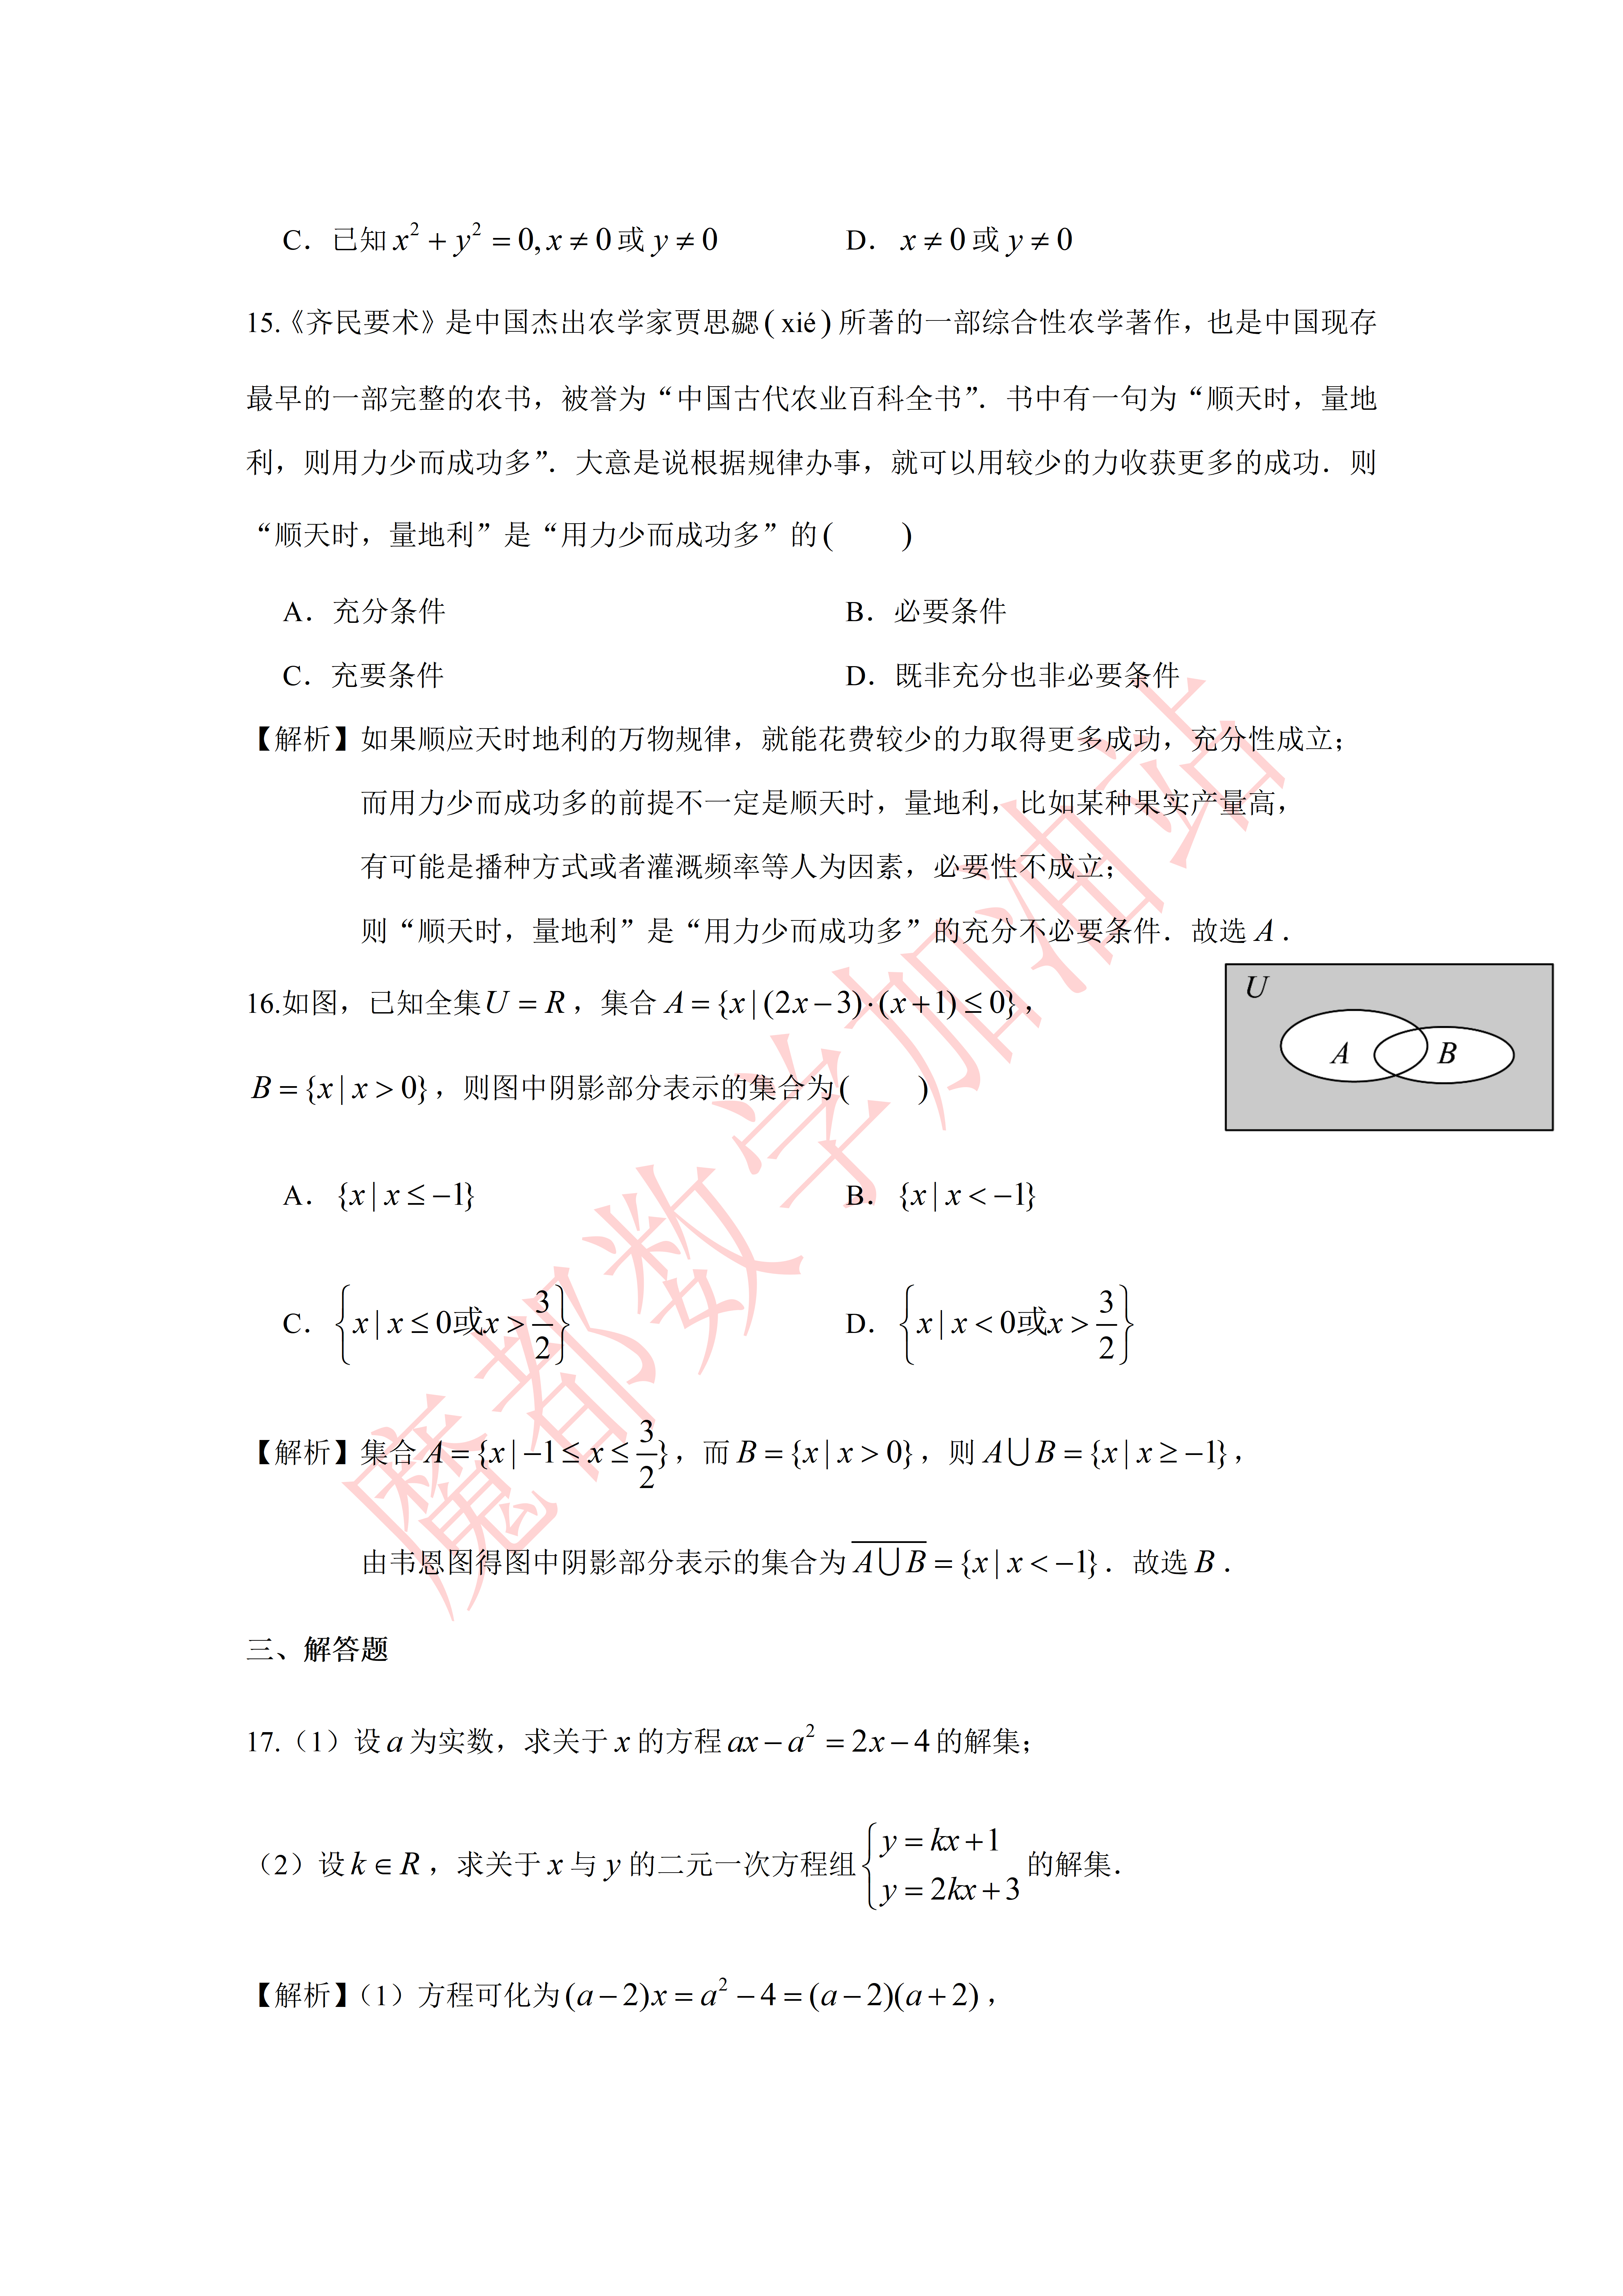
\includegraphics[width=.34\linewidth,trim=3586bp 3410bp 196bp 2818bp,clip]{../原图/高一52_回民中学_9月月考/04.png}
\end{center}

\keepwithprev
A. $\{x\mid x\leqslant-1\}$\qquad B. $\{x\mid x<-1\}$

C. $\left\{x\mid x\leqslant0\text{ 或 }x>\dfrac32\right\}$\qquad D. $\left\{x\mid x<0\text{ 或 }x>\dfrac32\right\}$

\ifanswer
\solbegin
\step{集合 $A=\left\{x\mid-1\leqslant x\leqslant\dfrac32\right\}$，而 $B=\{x\mid x>0\}$，则 $A\cup B=\{x\mid x\geqslant-1\}$，}
\step{由韦恩图得图中阴影部分表示的集合为 $\overline{A\cup B}=\{x\mid x<-1\}$．故选 $B$．}
\solend
\fi

\end{enumerate}

\bigsec{三、解答题}

\begin{enumerate}
\setcounter{enumi}{16}

\item （1）设 $a$ 为实数，求关于 $x$ 的方程 $ax-a^2=2x-4$ 的解集；

（2）设 $k\in\R$，求关于 $x$ 与 $y$ 的二元一次方程组 $\begin{cases}y=kx+1\\y=2kx+3\end{cases}$ 的解集．

\ifanswer
\solbegin
\stepm{(1)}{方程可化为 $(a-2)x=a^2-4=(a-2)(a+2)$，}
\step{当 $a\neq2$ 时，方程的解为 $x=\dfrac{(a-2)(a+2)}{a-2}=a+2$，则解集为 $\{a+2\}$；}
\step{当 $a=2$ 时，方程为 $2x-4=2x-4$，对 $x$ 取一切实数均成立，}
\step{所以解集为 $\R$；}
\stepm{(2)}{$\begin{cases}y=kx+1\\y=2kx+3\end{cases}$，则 $kx+1=2kx+3,kx=-2$，}
\step{当 $k=0$ 时，等式不成立，无解；当 $k\neq0$ 时，$x=-\dfrac2k,y=-1$；}
\step{综上所述，当 $k=0$ 时，解集为 $\varnothing$；当 $k\neq0$ 时，解集为 $\left\{\left(-\dfrac2k,-1\right)\right\}$．}
\solend
\fi

\ansspace[6]

\item 已知命题 $p$：方程 $x^2+6x+m-1=0$ 有两个不等的负根；命题 $q$：方程 $9x^2+6x+m-2=0$ 无实根．

\begin{enumerate}[label=(\arabic*)]
\item 若 $p$ 为真命题，求实数 $m$ 的取值范围；
\item 若 $p,q$ 两命题一真一假，求实数 $m$ 的取值范围．
\end{enumerate}

\ifanswer
\solbegin
\stepm{(1)}{设方程 $x^2+6x+m-1=0$ 两根为 $x_1,x_2$，}
\step{则 $\begin{cases}\Delta>0\\ x_1+x_2<0\\ x_1x_2>0\end{cases}\Rightarrow\begin{cases}36-4(m-1)>0\\ -6<0\\ m-1>0\end{cases}\Rightarrow1<m<10$；}
\stepm{(2)}{若命题 $q$ 为真命题，则 $36-36(m-2)<0\Rightarrow m>3$，}
\step{从而当命题 $q$ 为假命题时，$m\leqslant3$；}
\step{又由（1）得 $p$ 为假命题时，$m\leqslant1$ 或 $m\geqslant10$；}
\step{则当 $p$ 为真命题，$q$ 为假命题时，得 $\begin{cases}1<m<10\\ m\leqslant3\end{cases}\Rightarrow1<m\leqslant3$；}
\step{当 $q$ 为真命题，$p$ 为假命题时，得 $\begin{cases}m\leqslant1\text{ 或 }m\geqslant10\\ m>3\end{cases}\Rightarrow m\geqslant10$；}
\step{综上，当 $p,q$ 两命题一真一假时，$1<m\leqslant3$ 或 $m\geqslant10$.}
\solend
\fi

\ansspace[6]

\item 证明下列两个命题：

\begin{enumerate}[label=(\arabic*)]
\item 设 $ab>0$，求证：$a>b$ 是 $\dfrac1a<\dfrac1b$ 的充要条件．
\item 已知 $a,b$ 为正数，$n$ 为正整数，求证：如果 $a^n>b^n$，那么 $a>b$．
\end{enumerate}

\ifanswer
\solbegin
\stepm{(1)}{先证充分性：因为 $ab>0$ 且 $a>b$，故 $a-b>0$，从而 $\dfrac{a-b}{ab}>0$，}
\step{即 $\dfrac1b-\dfrac1a>0$，即 $\dfrac1a<\dfrac1b$；}
\step{再证必要性：若 $\dfrac1a<\dfrac1b$，则 $\dfrac1a-\dfrac1b=\dfrac{b-a}{ab}<0$，}
\step{又因为 $ab>0$，所以 $b-a<0$，即 $a>b$．}
% 原卷如此，照录未改（第 19 题(1)此句末用全角句号“。”，全卷其余各题末句用“．”，
% 见文件头“原卷笔误/存疑”第 4 条）
\step{综上，$a>b$ 是 $\dfrac1a<\dfrac1b$ 的充要条件。}
\stepm{(2)}{令 $f(x)=x^n,n\in\N^*$，则由幂函数的性质得 $f(x)$ 在第一象限是严格增的，}
\step{而 $a^n>b^n$ 即意味着 $f(a)>f(b)$，且 $a,b$ 为正数，从而 $a>b$．}
\solend
\fi

\ansspace[8]

\item （1）求关于 $x$ 的不等式 $(m-2)x>1-m$ 的解集；

（2）求关于 $x$ 的不等式 $x^2-(a+1)x+a\leqslant0$ 的解集．

\ifanswer
\solbegin
\stepm{(1)}{由不等式 $(m-2)x>1-m$，}
\step{当 $m-2>0$ 时，即 $m>2$ 时，解得 $x>\dfrac{1-m}{m-2}$，}
\step{所以不等式的解集为 $\left(\dfrac{1-m}{m-2},+\infty\right)$；}
\step{当 $m-2=0$ 时，即 $m=2$ 时，不等式即为 $0>-1$ 恒成立，}
\step{即不等式的解集为 $\R$；}
\step{当 $m-2<0$ 时，即 $m<2$ 时，解得 $x<\dfrac{1-m}{m-2}$，}
\step{所以不等式的解集为 $\left(-\infty,\dfrac{1-m}{m-2}\right)$；}
\step{综上，当 $m>2$ 时，解集为 $\left(\dfrac{1-m}{m-2},+\infty\right)$；}
\step{当 $m=2$ 时，解集为 $\R$；}
\step{当 $m<2$ 时，解集为 $\left(-\infty,\dfrac{1-m}{m-2}\right)$．}
\stepm{(2)}{由不等式 $x^2-(a+1)x+a\leqslant0$，可化为 $(x-a)(x-1)\leqslant0$，}
\step{当 $a>1$ 时，解得 $1\leqslant x\leqslant a$，即不等式的解集为 $[1,a]$；}
\step{当 $a=1$ 时，不等式即为 $(x-1)^2\leqslant0$，解得 $x=1$，即不等式的解集为 $\{1\}$；}
\step{当 $a<1$ 时，解得 $a\leqslant x\leqslant1$，即不等式的解集为 $[a,1]$，}
\step{综上，当 $a>1$ 时，解集为 $[1,a]$；}
\step{当 $a=1$ 时，解集为 $\{1\}$；}
\step{当 $a<1$ 时，解集为 $[a,1]$．}
\solend
\fi

\ansspace[10]

\item 已知集合 $A=\{x\mid(x+2)(5-x)\geqslant0\}$，若集合 $B$ 满足 $A\cap B=\varnothing,A\cup B=[-2,7)$．

\begin{enumerate}[label=(\arabic*)]
\item 用区间表示集合 $B$；
\item 若集合 $B$ 是不等式 $-x^2+bx+c>0$ 的解集，求实数 $b,c$ 的值；
\item 已知全集为 $\R$，若关于 $x$ 的不等式 $-1<x-a\leqslant2$ 的解集为 $M$，且“$x\in\overline A$”是“$x\in M$”的必要非充分条件，求实数 $a$ 的取值范围．
\end{enumerate}

\ifanswer
\solbegin
\stepm{(1)}{由题意得 $(x+2)(5-x)\geqslant0\Leftrightarrow(x+2)(x-5)\leqslant0\Rightarrow-2\leqslant x\leqslant5$，}
\step{则 $A=[-2,5]$，又 $A\cap B=\varnothing,A\cup B=[-2,7)$，则 $B=(5,7)$；}
\stepm{(2)}{$-x^2+bx+c>0\Leftrightarrow x^2-bx-c<0$，则 $x^2-bx-c=0$ 两根为 $5,7$，}
\step{则由韦达定理得 $b=12,-c=35\Rightarrow c=-35$；}
\stepm{(3)}{由题意得 $M=(a-1,a+2],\overline A=(-\infty,-2)\cup(5,+\infty)$，}
\step{且“$x\in\overline A$”是“$x\in M$”的必要非充分条件，则 $M$ 是 $\overline A$ 的真子集，}
\step{从而 $a+2<-2$ 或 $a-1\geqslant5$，解得 $a<-4$ 或 $a\geqslant6$，}
\step{所以实数 $a$ 的取值范围为 $(-\infty,-4)\cup[6,+\infty)$．}
\solend
\fi

\ansspace*[10]

\end{enumerate}

\end{document}
"
%
% 原始材料：微信公众号“魔都数学加油站”文章，作者破晓，连载“27学年高一52”；
% 原文标题“27学年高一52——2026-2027年上海市回民中学高一上9月月考”；
% 原文链接：https://mp.weixin.qq.com/s/ndjyozrRQCLl4ba3J8uR7g。
% 该页面用 JS 渲染，未见明确发布日期；页面内时间戳约为 2026-10-06 21:19／21:38，本稿以该时刻记可得日期。
% 正文为 8 张 PNG 页：第 01—07 页 4762×6735，第 08 页 2560×3620（**同一篇各页分辨率不同**），
% 均按页序读取。8 页全为试卷正文页（卷首标题在第 1 页页顶，卷末解答题第 21 题解析止于第 8 页），
% 无封面页、目录页、二维码或宣传页。粉色斜排“魔都数学加油站”为卷面水印，与公众号页脚一并未录入。
%
% 卷首标题：照卷面印作“2026--2027 年回民中学高一上 9 月月考”（公众号标题中的“上海市”
% 卷面标题行没有，本稿照卷面），年份区间按全稿惯例排 en dash。原卷只有一行标题、无副标题。
%
% 篇幅与题号：原卷自第 3 题起编号（第 1、2 题不在本卷内）。填空题 3—12（10 题）、
% 选择题 13—16（4 题）、解答题 17—21（5 题），共 19 题。本稿沿用原节与原题号，
% 只改排为全稿统一的大节样式（原卷小节标题为“一、填空题”“二、选择题”“三、解答题”）。
%
% 讲评版：原卷每题下直接印【答案】或【解析】。**只印【答案】的 1 题**（第 3 题），本稿只给 \ans{}；
% **第 14 题没有任何【答案】/【解析】段**，答案“D”直接印在题干括号内（“应假设(  D  )”），
% 本稿按 高一37 第 13 题的成例把括号留空、答案另提为 \ans{$D$}；
% 其余 17 题都只印【解析】，按全稿口径这类题不另提 \ans{}——其中选择题第 13、15、16 题的结论
% 写在解析末句（“故选 A／A／B”），亦照录在解析内。
%
% 副标题：原卷未印副标题。本稿按“知识模块”口径标作“集合与常用逻辑用语、不等式”：
% 19 题中集合与常用逻辑用语 10 题（集合类 7 题——第 3、4、5、9、12、16、21 题；
% 逻辑类 3 题——第 6、14、15 题），不等式 9 题（含等式性质与一元二次方程：第 7、8、10、11、
% 13、17、18、19、20 题），两类均远超三分之一，故并标。口径同 高一46、高一47、高一48、高一51。
%
% 与原卷的排版差异：
%   ① 原卷每题下直接印【答案】/【解析】，本稿按全稿惯例将答案与解析置于答案版，试卷版保持干净；
%      第 14 题印在题干括号内的答案“D”同样移入 \ans{}，见上；
%   ② 原卷未印副标题，本稿按“知识模块”口径补出；
%   ③ 原卷填空横线约两个字宽，本稿按全稿惯例统一排 \blankline[4.4em]；
%      选择题的作答括号原卷排半角“(    )”，本稿按全稿惯例排 \mbox{（\quad）}；
%   ④ 原卷实数集、自然数集排斜体/粗体 $R$、$\mathbf{R}$、$N$，本稿按全稿惯例改用 $\R$、$\N$；
%      空集记号统一为 \varnothing；
%   ⑤ 第 8 题题干与解析两处“两个实数分别为 $x_1$、$x_2$”原卷即用顿号，第 10、13 题等处
%      原卷在数学式内用半角逗号（如 $x_1,x_2$、$a,b,c\in R$），两份均照录未强改；
%      句末句点按全稿惯例排西文句点，句中句点（第 9、12、15、21 题）照原卷排全角“．”；
%   ⑥ 第 17、20 题原卷把子问标号“（1）”排在该题题号同一行，本稿照原卷仍排同一行（同 高一34 的
%      做法）；第 18、19、21 题的子问原卷各自另起一行，本稿按全稿惯例用 enumerate 的 (1)(2)(3)；
%      解析中的子问标号一律用 \stepm{(1)}{…}；
%   ⑦ 第 16 题的韦恩图原卷排在题干与选项右侧的浮动位置，本稿居中排在题干之后、选项之前，
%      并加 \needvspace 整块推走（守卫写在 \item 之前）；图自原图第 4 页裁切（trim），不另存图片文件；
%   ⑧ 每道解答题原卷未留作答空白，本稿按全稿惯例加 \ansspace。
%
% 原卷笔误/存疑（均照录未改，正文对应处另有 % 注）：
%   1. 第 8 题题干与解析首行两处均作“两个实数分别为 $x_1$、$x_2$”，按文意应为“两个实数**根**”
%      （疑脱“根”字，第 10 题同位置作“两个实根分别是”）；
%   2. 第 4 题解析“满足条件的 $A$ 的个数为集合 $\{0,1,3\}$ 的真子集，即 7 个”，
%      “个数为……真子集”表述不严（应为“……的真子集的个数”）；$\{0,1,3\}$ 的真子集 7 个，结论无误；
%   3. 第 6 题解析第 2 行“当 $a=10,b=0.2$ 时，$a+b>2$，且 $ab>1$，所以 $a>1$，且 $b>1$ 不成立”
%      ——此处是举反例，“所以”按文意应为“但”（$a=10,b=0.2$ 与“$a>1$ 且 $b>1$”不成立之间是转折，
%      非因果）；
%   4. 第 19 题 (1) 解析末行“综上，$a>b$ 是 $\dfrac1a<\dfrac1b$ 的充要条件。”用全角句号“。”，
%      全卷其余各题末句均用“．”，体例不一，照录；
%   5. 第 20 题第 (1) 问解析先按 $m>2$、$m=2$、$m<2$ 三种情况各给出解集，末三行又“综上”重述一遍，
%      与原卷一致（内容重复，非笔误）；
%   6. 第 18 题题干第 (2) 问“若 $p,q$ 两命题一真一假”，正文照录原卷所用半角逗号（未改顿号）。
%
% 插图：1 张，自原图裁切（无 \begin{tikzpicture} 重排）：
%   · 第 16 题题干韦恩图（全集 $U$ 矩形内两相交椭圆 $A$、$B$，灰色为阴影部分）
%     ——原图第 04 页，原卷排于题干与选项右侧。
%     裁框：x 3594–4558、y 2826–3317（即矩形外框，四周各留 4px），
%     trim=3590bp 3414bp 200bp 2822bp（左／下／右／上），页宽 4762、页高 6735。
%
\documentclass[a4paper,11pt]{article}
\usepackage{common}

\begin{document}

\examtitlest[3]{2026--2027 年回民中学高一上 9 月月考}{集合与常用逻辑用语、不等式}

\bigsec{一、填空题}

\begin{enumerate}
\setcounter{enumi}{2}

\item 用列举法写出下列集合 $\{(x,y)\mid x+y=2,x\in\N,y\in\N\}=$\blankline[4.4em].

\ifanswer
\ans{$\{(0,2),(1,1),(2,0)\}$}
\fi

\item 设集合 $A$ 满足 $\{-1,2\}\sub A\subset\{-1,0,1,2,3\}$，则满足条件的 $A$ 有\blankline[4.4em]个.

\ifanswer
\solbegin
\step{满足条件的 $A$ 的个数为集合 $\{0,1,3\}$ 的真子集，即 $7$ 个.}
\solend
\fi

\item 已知集合 $A=\{2,(a+1)^2,a^2+2\}$，且 $1\in A$，则实数 $a$ 的值为\blankline[4.4em].

\ifanswer
\solbegin
\step{因为 $1\in A$，而 $a^2+2\geqslant2$，所以 $(a+1)^2=1$，解得 $a=0$ 或 $a=-2$，}
\step{$a=0$ 时，$a^2+2=2$，不合题意，$a=-2$ 时，$a^2+2=6$，满足题意，}
\step{所以 $a=-2$.}
\solend
\fi

\item 已知 $a,b$ 是实数，则“$a>1$，且 $b>1$”是“$a+b>2$，且 $ab>1$”的\blankline[4.4em]条件.

\ifanswer
\solbegin
\step{$a,b$ 是实数，则“$a>1$，且 $b>1$”$\Rightarrow$“$a+b>2$，且 $ab>1$”正确，}
% 原卷如此，照录未改（第 6 题解析此处作“所以 $a>1$，且 $b>1$ 不成立”，按文意为转折，
% 见文件头“原卷笔误/存疑”第 3 条）
\step{当 $a=10,b=0.2$ 时，$a+b>2$，且 $ab>1$，所以 $a>1$，且 $b>1$ 不成立，}
\step{即前者是推出后者，后者推不出前者，}
\step{所以“$a>1$，且 $b>1$”是“$a+b>2$，且 $ab>1$”的充分而不必要条件.}
\solend
\fi

\item 已知等式 $2x^2-3x-1=a(x-1)^2+b(x-1)+c$ 恒成立，其中 $a,b,c$ 为常数，则 $a+b-c=$\blankline[4.4em].

\ifanswer
\solbegin
\step{将等式右侧展开整理得 $a(x-1)^2+b(x-1)+c=ax^2+(-2a+b)x+(a-b+c)$，}
\step{左右两边多项式恒等，对应次数的系数必须相等：}
\step{则 $a=2,-2a+b=-3$，代入 $a=2$ 得 $b=1$，$a-b+c=-1$，}
\step{代入 $a=2,b=1$ 得 $c=-2$，得 $a+b-c=2+1-(-2)=5$.}
\solend
\fi

% 原卷如此，照录未改（第 8 题题干与解析首行两处“两个实数分别为”疑脱“根”字，
% 见文件头“原卷笔误/存疑”第 1 条）
\item 若关于 $x$ 的二次方程 $x^2+mx+4m^2-3=0$ 的两个实数分别为 $x_1$、$x_2$，且满足 $x_1+x_2=x_1x_2$，则实数 $m$ 的值为\blankline[4.4em].

\ifanswer
\solbegin
% 原卷如此，照录未改（此处“两个实数分别为”同题干，疑脱“根”字）
\step{二次方程 $x^2+mx+4m^2-3=0$ 的两个实数分别为 $x_1$、$x_2$，}
\step{则有 $\Delta=m^2-4(4m^2-3)\geqslant0$，变形得 $m^2\leqslant\dfrac45$，}
\step{则 $x_1+x_2=-m$，$x_1x_2=(4m^2-3)$，}
\step{若 $x_1+x_2=x_1x_2$，则有 $-m=4m^2-3$，解得 $m=-1$ 或 $\dfrac34$，}
\step{又 $m^2\leqslant\dfrac45$，则 $m=\dfrac34$.}
\solend
\fi

\item 设集合 $A=\{x\mid x^2=1\}$，$B=\{x\mid ax=1\}$．若 $A\cap B=B$，则实数 $a$ 的值为\blankline[4.4em].

\ifanswer
\solbegin
\step{集合 $A=\{x\mid x^2=1\}=\{-1,1\}$，$B=\{x\mid ax=1\}$，$A\cap B=B$，所以 $B\sub A$，}
\step{当 $a=0$ 时，$B=\varnothing$，成立；}
\step{当 $a\neq0$ 时，$B=\left\{\dfrac1a\right\}$，则 $\dfrac1a=-1$ 或 $\dfrac1a=1$，解得 $a=-1$ 或 $a=1$，}
\step{所以实数 $a$ 的值为 $0$ 或 $1$ 或 $-1$.}
\solend
\fi

\item 已知关于 $x$ 的一元二次方程 $x^2+3x-3=0$ 的两个实根分别是 $x_1,x_2$，则以 $-\dfrac1{x_1},-\dfrac1{x_2}$ 为根且二次项系数是 $1$ 的一元二次方程为\blankline[4.4em].

\ifanswer
\solbegin
\step{因为 $x_1,x_2$ 是一元二次方程 $x^2+3x-3=0$ 的两个实根，}
\step{所以 $x_1+x_2=-3,x_1x_2=-3$，}
\step{所以 $-\dfrac1{x_1}+\left(-\dfrac1{x_2}\right)=-\dfrac{x_1+x_2}{x_1x_2}=-1$，$-\dfrac1{x_1}\cdot\left(-\dfrac1{x_2}\right)=\dfrac1{x_1x_2}=-\dfrac13$，}
\step{所以一元二次方程为 $x^2+x-\dfrac13=0$.}
\solend
\fi

\item 若关于 $x$ 的不等式 $(a-2)x^2+2(a-2)x-4<0$ 的解集是 $\R$，则实数 $a$ 的取值范围是\blankline[4.4em].

\ifanswer
\solbegin
\step{当 $a=2$ 时，不等式化为 $-4<0$ 对于任意实数 $x$ 都成立，因此 $a=2$ 满足题意；}
\step{当 $a\neq2$ 时，要使关于 $x$ 的不等式 $(a-2)x^2+2(a-2)x-4<0$ 的解集为 $\R$，}
\step{则 $\begin{cases}a-2<0\\ \Delta=4(a-2)^2+16(a-2)<0\end{cases}$，解得 $-2<a<2$．}
\step{综上，$a$ 的取值范围为 $(-2,2]$．}
\solend
\fi

\item 设非空集合 $A$、$B$，定义 $A\times B=\{x\mid x\in(A\cup B),x\notin(A\cap B)\}$．已知 $A=\{x\mid0\leqslant x\leqslant2\}$，$B=\{y\mid y\geqslant0\}$，则 $A\times B=$\blankline[4.4em].

\ifanswer
\solbegin
\step{由于 $A=\{x\mid0\leqslant x\leqslant2\}$，$B=\{y\mid y\geqslant0\}=\{x\mid x\geqslant0\}$，}
\step{所以 $A\cup B=\{x\mid x\geqslant0\}$，$A\cap B=\{x\mid0\leqslant x\leqslant2\}$，故 $A\times B=\{x\mid x>2\}$．}
\solend
\fi

\end{enumerate}

\bigsec{二、选择题}

\begin{enumerate}
\setcounter{enumi}{12}

\item 已知 $a,b,c\in\R$ 且 $a>b$，则下列不等式一定成立的是\mbox{（\quad）}

\keepwithprev
A. $\dfrac{a}{c^2+1}>\dfrac{b}{c^2+1}$\qquad B. $\dfrac1a<\dfrac1b$

C. $ac>bc$\qquad D. $a^2>b^2$

\ifanswer
\solbegin
\step{对于 A：因为 $c^2+1>0$ 恒成立，且 $a>b$，所以 $\dfrac{a}{c^2+1}>\dfrac{b}{c^2+1}$ 一定成立，}
\step{所以 A 正确；}
\step{对于 B：当 $a=1,b=-1$ 时，满足 $a>b$，此时 $\dfrac1a=1>\dfrac1b=-1$，所以 B 错误；}
\step{对于 C：当 $c<0$ 时，由 $a>b$，得 $ac<bc$，所以 C 错误；}
\step{对于 D：当 $a=1,b=-2$ 时，满足 $a>b$，此时 $a^2=1<b^2=4$，所以 D 错误；}
\step{故选 $A$．}
\solend
\fi

% 注：本题的答案“D”原卷直接印在题干末尾的括号内（“应假设(  D  )”），且没有单独的
%     【答案】/【解析】段，本稿按 高一37 第 13 题的成例把括号留空、另提为 \ans{}，
%     见文件头“与原卷的排版差异”①。
\item 用反证法证明：“已知 $x,y\in\R$,$x^2+y^2=0$，求证：$x=y=0$”时，应假设\mbox{（\quad）}

\keepwithprev
A. 已知 $x^2+y^2=0,x\neq0$ 且 $y\neq0$\qquad B. $x\neq0$ 且 $y\neq0$

C. 已知 $x^2+y^2=0,x\neq0$ 或 $y\neq0$\qquad D. $x\neq0$ 或 $y\neq0$

\ans{$D$}

\item 《齐民要术》是中国杰出农学家贾思勰（xié）所著的一部综合性农学著作，也是中国现存最早的一部完整的农书，被誉为“中国古代农业百科全书”．书中有一句为“顺天时，量地利，则用力少而成功多”．大意是说根据规律办事，就可以用较少的力收获更多的成功．则“顺天时，量地利”是“用力少而成功多”的\mbox{（\quad）}

\keepwithprev
A. 充分条件\qquad B. 必要条件

C. 充要条件\qquad D. 既非充分也非必要条件

\ifanswer
\solbegin
\step{如果顺应天时地利的万物规律，就能花费较少的力取得更多成功，充分性成立；}
\step{而用力少而成功多的前提不一定是顺天时，量地利，比如某种果实产量高，}
\step{有可能是播种方式或者灌溉频率等人为因素，必要性不成立；}
\step{则“顺天时，量地利”是“用力少而成功多”的充分不必要条件．故选 $A$．}
\solend
\fi

\needvspace{13\baselineskip}

\item 如图，已知全集 $U=\R$，集合 $A=\{x\mid(2x-3)\cdot(x+1)\leqslant0\}$，$B=\{x\mid x>0\}$，则图中阴影部分表示的集合为\mbox{（\quad）}

\begin{center}
% 原图第 4 页题干韦恩图直接裁取（原卷排于题干与选项右侧）。
% 裁框取矩形外框 x 3590–4558、y 2822–3321，再向外各留 4px（即 x 3586–4562、y 2818–3325），
% trim=左 3586bp／下 3410bp／右 196bp／上 2818bp（页宽 4762、页高 6735）。
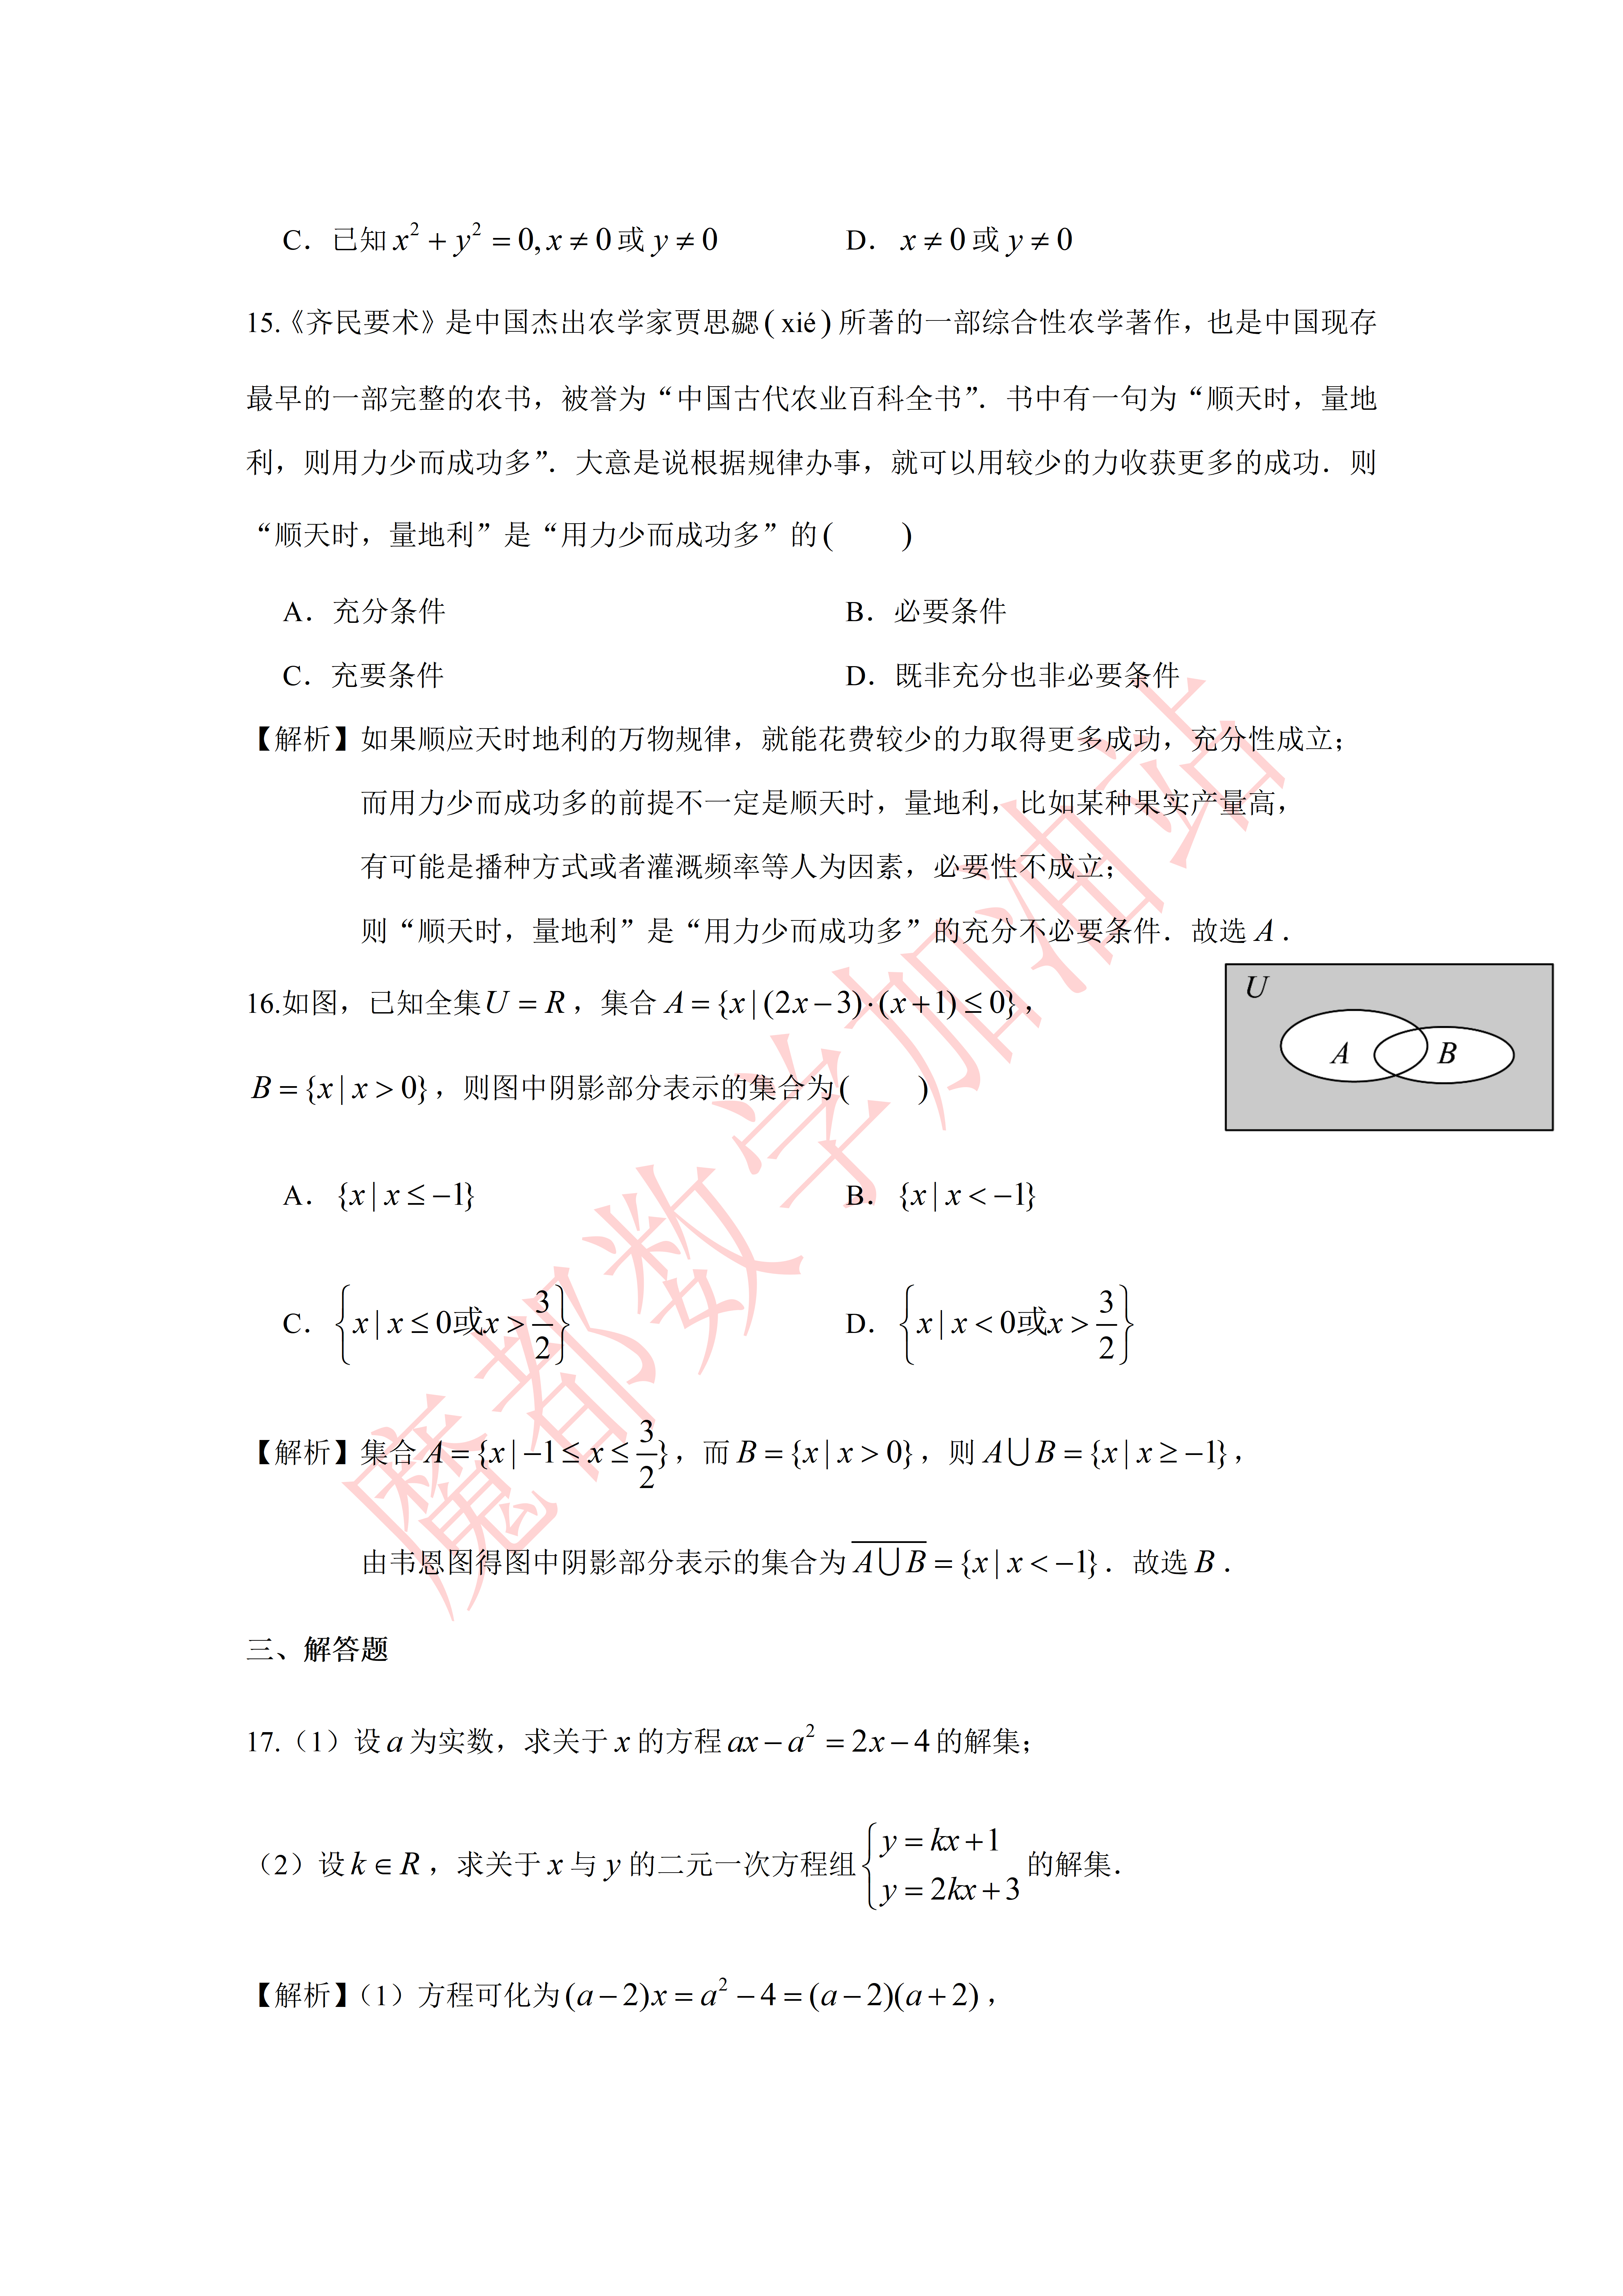
\includegraphics[width=.34\linewidth,trim=3586bp 3410bp 196bp 2818bp,clip]{../原图/高一52_回民中学_9月月考/04.png}
\end{center}

\keepwithprev
A. $\{x\mid x\leqslant-1\}$\qquad B. $\{x\mid x<-1\}$

C. $\left\{x\mid x\leqslant0\text{ 或 }x>\dfrac32\right\}$\qquad D. $\left\{x\mid x<0\text{ 或 }x>\dfrac32\right\}$

\ifanswer
\solbegin
\step{集合 $A=\left\{x\mid-1\leqslant x\leqslant\dfrac32\right\}$，而 $B=\{x\mid x>0\}$，则 $A\cup B=\{x\mid x\geqslant-1\}$，}
\step{由韦恩图得图中阴影部分表示的集合为 $\overline{A\cup B}=\{x\mid x<-1\}$．故选 $B$．}
\solend
\fi

\end{enumerate}

\bigsec{三、解答题}

\begin{enumerate}
\setcounter{enumi}{16}

\item （1）设 $a$ 为实数，求关于 $x$ 的方程 $ax-a^2=2x-4$ 的解集；

（2）设 $k\in\R$，求关于 $x$ 与 $y$ 的二元一次方程组 $\begin{cases}y=kx+1\\y=2kx+3\end{cases}$ 的解集．

\ifanswer
\solbegin
\stepm{(1)}{方程可化为 $(a-2)x=a^2-4=(a-2)(a+2)$，}
\step{当 $a\neq2$ 时，方程的解为 $x=\dfrac{(a-2)(a+2)}{a-2}=a+2$，则解集为 $\{a+2\}$；}
\step{当 $a=2$ 时，方程为 $2x-4=2x-4$，对 $x$ 取一切实数均成立，}
\step{所以解集为 $\R$；}
\stepm{(2)}{$\begin{cases}y=kx+1\\y=2kx+3\end{cases}$，则 $kx+1=2kx+3,kx=-2$，}
\step{当 $k=0$ 时，等式不成立，无解；当 $k\neq0$ 时，$x=-\dfrac2k,y=-1$；}
\step{综上所述，当 $k=0$ 时，解集为 $\varnothing$；当 $k\neq0$ 时，解集为 $\left\{\left(-\dfrac2k,-1\right)\right\}$．}
\solend
\fi

\ansspace[6]

\item 已知命题 $p$：方程 $x^2+6x+m-1=0$ 有两个不等的负根；命题 $q$：方程 $9x^2+6x+m-2=0$ 无实根．

\begin{enumerate}[label=(\arabic*)]
\item 若 $p$ 为真命题，求实数 $m$ 的取值范围；
\item 若 $p,q$ 两命题一真一假，求实数 $m$ 的取值范围．
\end{enumerate}

\ifanswer
\solbegin
\stepm{(1)}{设方程 $x^2+6x+m-1=0$ 两根为 $x_1,x_2$，}
\step{则 $\begin{cases}\Delta>0\\ x_1+x_2<0\\ x_1x_2>0\end{cases}\Rightarrow\begin{cases}36-4(m-1)>0\\ -6<0\\ m-1>0\end{cases}\Rightarrow1<m<10$；}
\stepm{(2)}{若命题 $q$ 为真命题，则 $36-36(m-2)<0\Rightarrow m>3$，}
\step{从而当命题 $q$ 为假命题时，$m\leqslant3$；}
\step{又由（1）得 $p$ 为假命题时，$m\leqslant1$ 或 $m\geqslant10$；}
\step{则当 $p$ 为真命题，$q$ 为假命题时，得 $\begin{cases}1<m<10\\ m\leqslant3\end{cases}\Rightarrow1<m\leqslant3$；}
\step{当 $q$ 为真命题，$p$ 为假命题时，得 $\begin{cases}m\leqslant1\text{ 或 }m\geqslant10\\ m>3\end{cases}\Rightarrow m\geqslant10$；}
\step{综上，当 $p,q$ 两命题一真一假时，$1<m\leqslant3$ 或 $m\geqslant10$.}
\solend
\fi

\ansspace[6]

\item 证明下列两个命题：

\begin{enumerate}[label=(\arabic*)]
\item 设 $ab>0$，求证：$a>b$ 是 $\dfrac1a<\dfrac1b$ 的充要条件．
\item 已知 $a,b$ 为正数，$n$ 为正整数，求证：如果 $a^n>b^n$，那么 $a>b$．
\end{enumerate}

\ifanswer
\solbegin
\stepm{(1)}{先证充分性：因为 $ab>0$ 且 $a>b$，故 $a-b>0$，从而 $\dfrac{a-b}{ab}>0$，}
\step{即 $\dfrac1b-\dfrac1a>0$，即 $\dfrac1a<\dfrac1b$；}
\step{再证必要性：若 $\dfrac1a<\dfrac1b$，则 $\dfrac1a-\dfrac1b=\dfrac{b-a}{ab}<0$，}
\step{又因为 $ab>0$，所以 $b-a<0$，即 $a>b$．}
% 原卷如此，照录未改（第 19 题(1)此句末用全角句号“。”，全卷其余各题末句用“．”，
% 见文件头“原卷笔误/存疑”第 4 条）
\step{综上，$a>b$ 是 $\dfrac1a<\dfrac1b$ 的充要条件。}
\stepm{(2)}{令 $f(x)=x^n,n\in\N^*$，则由幂函数的性质得 $f(x)$ 在第一象限是严格增的，}
\step{而 $a^n>b^n$ 即意味着 $f(a)>f(b)$，且 $a,b$ 为正数，从而 $a>b$．}
\solend
\fi

\ansspace[8]

\item （1）求关于 $x$ 的不等式 $(m-2)x>1-m$ 的解集；

（2）求关于 $x$ 的不等式 $x^2-(a+1)x+a\leqslant0$ 的解集．

\ifanswer
\solbegin
\stepm{(1)}{由不等式 $(m-2)x>1-m$，}
\step{当 $m-2>0$ 时，即 $m>2$ 时，解得 $x>\dfrac{1-m}{m-2}$，}
\step{所以不等式的解集为 $\left(\dfrac{1-m}{m-2},+\infty\right)$；}
\step{当 $m-2=0$ 时，即 $m=2$ 时，不等式即为 $0>-1$ 恒成立，}
\step{即不等式的解集为 $\R$；}
\step{当 $m-2<0$ 时，即 $m<2$ 时，解得 $x<\dfrac{1-m}{m-2}$，}
\step{所以不等式的解集为 $\left(-\infty,\dfrac{1-m}{m-2}\right)$；}
\step{综上，当 $m>2$ 时，解集为 $\left(\dfrac{1-m}{m-2},+\infty\right)$；}
\step{当 $m=2$ 时，解集为 $\R$；}
\step{当 $m<2$ 时，解集为 $\left(-\infty,\dfrac{1-m}{m-2}\right)$．}
\stepm{(2)}{由不等式 $x^2-(a+1)x+a\leqslant0$，可化为 $(x-a)(x-1)\leqslant0$，}
\step{当 $a>1$ 时，解得 $1\leqslant x\leqslant a$，即不等式的解集为 $[1,a]$；}
\step{当 $a=1$ 时，不等式即为 $(x-1)^2\leqslant0$，解得 $x=1$，即不等式的解集为 $\{1\}$；}
\step{当 $a<1$ 时，解得 $a\leqslant x\leqslant1$，即不等式的解集为 $[a,1]$，}
\step{综上，当 $a>1$ 时，解集为 $[1,a]$；}
\step{当 $a=1$ 时，解集为 $\{1\}$；}
\step{当 $a<1$ 时，解集为 $[a,1]$．}
\solend
\fi

\ansspace[10]

\item 已知集合 $A=\{x\mid(x+2)(5-x)\geqslant0\}$，若集合 $B$ 满足 $A\cap B=\varnothing,A\cup B=[-2,7)$．

\begin{enumerate}[label=(\arabic*)]
\item 用区间表示集合 $B$；
\item 若集合 $B$ 是不等式 $-x^2+bx+c>0$ 的解集，求实数 $b,c$ 的值；
\item 已知全集为 $\R$，若关于 $x$ 的不等式 $-1<x-a\leqslant2$ 的解集为 $M$，且“$x\in\overline A$”是“$x\in M$”的必要非充分条件，求实数 $a$ 的取值范围．
\end{enumerate}

\ifanswer
\solbegin
\stepm{(1)}{由题意得 $(x+2)(5-x)\geqslant0\Leftrightarrow(x+2)(x-5)\leqslant0\Rightarrow-2\leqslant x\leqslant5$，}
\step{则 $A=[-2,5]$，又 $A\cap B=\varnothing,A\cup B=[-2,7)$，则 $B=(5,7)$；}
\stepm{(2)}{$-x^2+bx+c>0\Leftrightarrow x^2-bx-c<0$，则 $x^2-bx-c=0$ 两根为 $5,7$，}
\step{则由韦达定理得 $b=12,-c=35\Rightarrow c=-35$；}
\stepm{(3)}{由题意得 $M=(a-1,a+2],\overline A=(-\infty,-2)\cup(5,+\infty)$，}
\step{且“$x\in\overline A$”是“$x\in M$”的必要非充分条件，则 $M$ 是 $\overline A$ 的真子集，}
\step{从而 $a+2<-2$ 或 $a-1\geqslant5$，解得 $a<-4$ 或 $a\geqslant6$，}
\step{所以实数 $a$ 的取值范围为 $(-\infty,-4)\cup[6,+\infty)$．}
\solend
\fi

\ansspace*[10]

\end{enumerate}

\end{document}
"
%
% 原始材料：微信公众号“魔都数学加油站”文章，作者破晓，连载“27学年高一52”；
% 原文标题“27学年高一52——2026-2027年上海市回民中学高一上9月月考”；
% 原文链接：https://mp.weixin.qq.com/s/ndjyozrRQCLl4ba3J8uR7g。
% 该页面用 JS 渲染，未见明确发布日期；页面内时间戳约为 2026-10-06 21:19／21:38，本稿以该时刻记可得日期。
% 正文为 8 张 PNG 页：第 01—07 页 4762×6735，第 08 页 2560×3620（**同一篇各页分辨率不同**），
% 均按页序读取。8 页全为试卷正文页（卷首标题在第 1 页页顶，卷末解答题第 21 题解析止于第 8 页），
% 无封面页、目录页、二维码或宣传页。粉色斜排“魔都数学加油站”为卷面水印，与公众号页脚一并未录入。
%
% 卷首标题：照卷面印作“2026--2027 年回民中学高一上 9 月月考”（公众号标题中的“上海市”
% 卷面标题行没有，本稿照卷面），年份区间按全稿惯例排 en dash。原卷只有一行标题、无副标题。
%
% 篇幅与题号：原卷自第 3 题起编号（第 1、2 题不在本卷内）。填空题 3—12（10 题）、
% 选择题 13—16（4 题）、解答题 17—21（5 题），共 19 题。本稿沿用原节与原题号，
% 只改排为全稿统一的大节样式（原卷小节标题为“一、填空题”“二、选择题”“三、解答题”）。
%
% 讲评版：原卷每题下直接印【答案】或【解析】。**只印【答案】的 1 题**（第 3 题），本稿只给 \ans{}；
% **第 14 题没有任何【答案】/【解析】段**，答案“D”直接印在题干括号内（“应假设(  D  )”），
% 本稿按 高一37 第 13 题的成例把括号留空、答案另提为 \ans{$D$}；
% 其余 17 题都只印【解析】，按全稿口径这类题不另提 \ans{}——其中选择题第 13、15、16 题的结论
% 写在解析末句（“故选 A／A／B”），亦照录在解析内。
%
% 副标题：原卷未印副标题。本稿按“知识模块”口径标作“集合与常用逻辑用语、不等式”：
% 19 题中集合与常用逻辑用语 10 题（集合类 7 题——第 3、4、5、9、12、16、21 题；
% 逻辑类 3 题——第 6、14、15 题），不等式 9 题（含等式性质与一元二次方程：第 7、8、10、11、
% 13、17、18、19、20 题），两类均远超三分之一，故并标。口径同 高一46、高一47、高一48、高一51。
%
% 与原卷的排版差异：
%   ① 原卷每题下直接印【答案】/【解析】，本稿按全稿惯例将答案与解析置于答案版，试卷版保持干净；
%      第 14 题印在题干括号内的答案“D”同样移入 \ans{}，见上；
%   ② 原卷未印副标题，本稿按“知识模块”口径补出；
%   ③ 原卷填空横线约两个字宽，本稿按全稿惯例统一排 \blankline[4.4em]；
%      选择题的作答括号原卷排半角“(    )”，本稿按全稿惯例排 \mbox{（\quad）}；
%   ④ 原卷实数集、自然数集排斜体/粗体 $R$、$\mathbf{R}$、$N$，本稿按全稿惯例改用 $\R$、$\N$；
%      空集记号统一为 \varnothing；
%   ⑤ 第 8 题题干与解析两处“两个实数分别为 $x_1$、$x_2$”原卷即用顿号，第 10、13 题等处
%      原卷在数学式内用半角逗号（如 $x_1,x_2$、$a,b,c\in R$），两份均照录未强改；
%      句末句点按全稿惯例排西文句点，句中句点（第 9、12、15、21 题）照原卷排全角“．”；
%   ⑥ 第 17、20 题原卷把子问标号“（1）”排在该题题号同一行，本稿照原卷仍排同一行（同 高一34 的
%      做法）；第 18、19、21 题的子问原卷各自另起一行，本稿按全稿惯例用 enumerate 的 (1)(2)(3)；
%      解析中的子问标号一律用 \stepm{(1)}{…}；
%   ⑦ 第 16 题的韦恩图原卷排在题干与选项右侧的浮动位置，本稿居中排在题干之后、选项之前，
%      并加 \needvspace 整块推走（守卫写在 \item 之前）；图自原图第 4 页裁切（trim），不另存图片文件；
%   ⑧ 每道解答题原卷未留作答空白，本稿按全稿惯例加 \ansspace。
%
% 原卷笔误/存疑（均照录未改，正文对应处另有 % 注）：
%   1. 第 8 题题干与解析首行两处均作“两个实数分别为 $x_1$、$x_2$”，按文意应为“两个实数**根**”
%      （疑脱“根”字，第 10 题同位置作“两个实根分别是”）；
%   2. 第 4 题解析“满足条件的 $A$ 的个数为集合 $\{0,1,3\}$ 的真子集，即 7 个”，
%      “个数为……真子集”表述不严（应为“……的真子集的个数”）；$\{0,1,3\}$ 的真子集 7 个，结论无误；
%   3. 第 6 题解析第 2 行“当 $a=10,b=0.2$ 时，$a+b>2$，且 $ab>1$，所以 $a>1$，且 $b>1$ 不成立”
%      ——此处是举反例，“所以”按文意应为“但”（$a=10,b=0.2$ 与“$a>1$ 且 $b>1$”不成立之间是转折，
%      非因果）；
%   4. 第 19 题 (1) 解析末行“综上，$a>b$ 是 $\dfrac1a<\dfrac1b$ 的充要条件。”用全角句号“。”，
%      全卷其余各题末句均用“．”，体例不一，照录；
%   5. 第 20 题第 (1) 问解析先按 $m>2$、$m=2$、$m<2$ 三种情况各给出解集，末三行又“综上”重述一遍，
%      与原卷一致（内容重复，非笔误）；
%   6. 第 18 题题干第 (2) 问“若 $p,q$ 两命题一真一假”，正文照录原卷所用半角逗号（未改顿号）。
%
% 插图：1 张，自原图裁切（无 \begin{tikzpicture} 重排）：
%   · 第 16 题题干韦恩图（全集 $U$ 矩形内两相交椭圆 $A$、$B$，灰色为阴影部分）
%     ——原图第 04 页，原卷排于题干与选项右侧。
%     裁框：x 3594–4558、y 2826–3317（即矩形外框，四周各留 4px），
%     trim=3590bp 3414bp 200bp 2822bp（左／下／右／上），页宽 4762、页高 6735。
%
\documentclass[a4paper,11pt]{article}
\usepackage{common}

\begin{document}

\examtitlest[3]{2026--2027 年回民中学高一上 9 月月考}{集合与常用逻辑用语、不等式}

\bigsec{一、填空题}

\begin{enumerate}
\setcounter{enumi}{2}

\item 用列举法写出下列集合 $\{(x,y)\mid x+y=2,x\in\N,y\in\N\}=$\blankline[4.4em].

\ifanswer
\ans{$\{(0,2),(1,1),(2,0)\}$}
\fi

\item 设集合 $A$ 满足 $\{-1,2\}\sub A\subset\{-1,0,1,2,3\}$，则满足条件的 $A$ 有\blankline[4.4em]个.

\ifanswer
\solbegin
\step{满足条件的 $A$ 的个数为集合 $\{0,1,3\}$ 的真子集，即 $7$ 个.}
\solend
\fi

\item 已知集合 $A=\{2,(a+1)^2,a^2+2\}$，且 $1\in A$，则实数 $a$ 的值为\blankline[4.4em].

\ifanswer
\solbegin
\step{因为 $1\in A$，而 $a^2+2\geqslant2$，所以 $(a+1)^2=1$，解得 $a=0$ 或 $a=-2$，}
\step{$a=0$ 时，$a^2+2=2$，不合题意，$a=-2$ 时，$a^2+2=6$，满足题意，}
\step{所以 $a=-2$.}
\solend
\fi

\item 已知 $a,b$ 是实数，则“$a>1$，且 $b>1$”是“$a+b>2$，且 $ab>1$”的\blankline[4.4em]条件.

\ifanswer
\solbegin
\step{$a,b$ 是实数，则“$a>1$，且 $b>1$”$\Rightarrow$“$a+b>2$，且 $ab>1$”正确，}
% 原卷如此，照录未改（第 6 题解析此处作“所以 $a>1$，且 $b>1$ 不成立”，按文意为转折，
% 见文件头“原卷笔误/存疑”第 3 条）
\step{当 $a=10,b=0.2$ 时，$a+b>2$，且 $ab>1$，所以 $a>1$，且 $b>1$ 不成立，}
\step{即前者是推出后者，后者推不出前者，}
\step{所以“$a>1$，且 $b>1$”是“$a+b>2$，且 $ab>1$”的充分而不必要条件.}
\solend
\fi

\item 已知等式 $2x^2-3x-1=a(x-1)^2+b(x-1)+c$ 恒成立，其中 $a,b,c$ 为常数，则 $a+b-c=$\blankline[4.4em].

\ifanswer
\solbegin
\step{将等式右侧展开整理得 $a(x-1)^2+b(x-1)+c=ax^2+(-2a+b)x+(a-b+c)$，}
\step{左右两边多项式恒等，对应次数的系数必须相等：}
\step{则 $a=2,-2a+b=-3$，代入 $a=2$ 得 $b=1$，$a-b+c=-1$，}
\step{代入 $a=2,b=1$ 得 $c=-2$，得 $a+b-c=2+1-(-2)=5$.}
\solend
\fi

% 原卷如此，照录未改（第 8 题题干与解析首行两处“两个实数分别为”疑脱“根”字，
% 见文件头“原卷笔误/存疑”第 1 条）
\item 若关于 $x$ 的二次方程 $x^2+mx+4m^2-3=0$ 的两个实数分别为 $x_1$、$x_2$，且满足 $x_1+x_2=x_1x_2$，则实数 $m$ 的值为\blankline[4.4em].

\ifanswer
\solbegin
% 原卷如此，照录未改（此处“两个实数分别为”同题干，疑脱“根”字）
\step{二次方程 $x^2+mx+4m^2-3=0$ 的两个实数分别为 $x_1$、$x_2$，}
\step{则有 $\Delta=m^2-4(4m^2-3)\geqslant0$，变形得 $m^2\leqslant\dfrac45$，}
\step{则 $x_1+x_2=-m$，$x_1x_2=(4m^2-3)$，}
\step{若 $x_1+x_2=x_1x_2$，则有 $-m=4m^2-3$，解得 $m=-1$ 或 $\dfrac34$，}
\step{又 $m^2\leqslant\dfrac45$，则 $m=\dfrac34$.}
\solend
\fi

\item 设集合 $A=\{x\mid x^2=1\}$，$B=\{x\mid ax=1\}$．若 $A\cap B=B$，则实数 $a$ 的值为\blankline[4.4em].

\ifanswer
\solbegin
\step{集合 $A=\{x\mid x^2=1\}=\{-1,1\}$，$B=\{x\mid ax=1\}$，$A\cap B=B$，所以 $B\sub A$，}
\step{当 $a=0$ 时，$B=\varnothing$，成立；}
\step{当 $a\neq0$ 时，$B=\left\{\dfrac1a\right\}$，则 $\dfrac1a=-1$ 或 $\dfrac1a=1$，解得 $a=-1$ 或 $a=1$，}
\step{所以实数 $a$ 的值为 $0$ 或 $1$ 或 $-1$.}
\solend
\fi

\item 已知关于 $x$ 的一元二次方程 $x^2+3x-3=0$ 的两个实根分别是 $x_1,x_2$，则以 $-\dfrac1{x_1},-\dfrac1{x_2}$ 为根且二次项系数是 $1$ 的一元二次方程为\blankline[4.4em].

\ifanswer
\solbegin
\step{因为 $x_1,x_2$ 是一元二次方程 $x^2+3x-3=0$ 的两个实根，}
\step{所以 $x_1+x_2=-3,x_1x_2=-3$，}
\step{所以 $-\dfrac1{x_1}+\left(-\dfrac1{x_2}\right)=-\dfrac{x_1+x_2}{x_1x_2}=-1$，$-\dfrac1{x_1}\cdot\left(-\dfrac1{x_2}\right)=\dfrac1{x_1x_2}=-\dfrac13$，}
\step{所以一元二次方程为 $x^2+x-\dfrac13=0$.}
\solend
\fi

\item 若关于 $x$ 的不等式 $(a-2)x^2+2(a-2)x-4<0$ 的解集是 $\R$，则实数 $a$ 的取值范围是\blankline[4.4em].

\ifanswer
\solbegin
\step{当 $a=2$ 时，不等式化为 $-4<0$ 对于任意实数 $x$ 都成立，因此 $a=2$ 满足题意；}
\step{当 $a\neq2$ 时，要使关于 $x$ 的不等式 $(a-2)x^2+2(a-2)x-4<0$ 的解集为 $\R$，}
\step{则 $\begin{cases}a-2<0\\ \Delta=4(a-2)^2+16(a-2)<0\end{cases}$，解得 $-2<a<2$．}
\step{综上，$a$ 的取值范围为 $(-2,2]$．}
\solend
\fi

\item 设非空集合 $A$、$B$，定义 $A\times B=\{x\mid x\in(A\cup B),x\notin(A\cap B)\}$．已知 $A=\{x\mid0\leqslant x\leqslant2\}$，$B=\{y\mid y\geqslant0\}$，则 $A\times B=$\blankline[4.4em].

\ifanswer
\solbegin
\step{由于 $A=\{x\mid0\leqslant x\leqslant2\}$，$B=\{y\mid y\geqslant0\}=\{x\mid x\geqslant0\}$，}
\step{所以 $A\cup B=\{x\mid x\geqslant0\}$，$A\cap B=\{x\mid0\leqslant x\leqslant2\}$，故 $A\times B=\{x\mid x>2\}$．}
\solend
\fi

\end{enumerate}

\bigsec{二、选择题}

\begin{enumerate}
\setcounter{enumi}{12}

\item 已知 $a,b,c\in\R$ 且 $a>b$，则下列不等式一定成立的是\mbox{（\quad）}

\keepwithprev
A. $\dfrac{a}{c^2+1}>\dfrac{b}{c^2+1}$\qquad B. $\dfrac1a<\dfrac1b$

C. $ac>bc$\qquad D. $a^2>b^2$

\ifanswer
\solbegin
\step{对于 A：因为 $c^2+1>0$ 恒成立，且 $a>b$，所以 $\dfrac{a}{c^2+1}>\dfrac{b}{c^2+1}$ 一定成立，}
\step{所以 A 正确；}
\step{对于 B：当 $a=1,b=-1$ 时，满足 $a>b$，此时 $\dfrac1a=1>\dfrac1b=-1$，所以 B 错误；}
\step{对于 C：当 $c<0$ 时，由 $a>b$，得 $ac<bc$，所以 C 错误；}
\step{对于 D：当 $a=1,b=-2$ 时，满足 $a>b$，此时 $a^2=1<b^2=4$，所以 D 错误；}
\step{故选 $A$．}
\solend
\fi

% 注：本题的答案“D”原卷直接印在题干末尾的括号内（“应假设(  D  )”），且没有单独的
%     【答案】/【解析】段，本稿按 高一37 第 13 题的成例把括号留空、另提为 \ans{}，
%     见文件头“与原卷的排版差异”①。
\item 用反证法证明：“已知 $x,y\in\R$,$x^2+y^2=0$，求证：$x=y=0$”时，应假设\mbox{（\quad）}

\keepwithprev
A. 已知 $x^2+y^2=0,x\neq0$ 且 $y\neq0$\qquad B. $x\neq0$ 且 $y\neq0$

C. 已知 $x^2+y^2=0,x\neq0$ 或 $y\neq0$\qquad D. $x\neq0$ 或 $y\neq0$

\ans{$D$}

\item 《齐民要术》是中国杰出农学家贾思勰（xié）所著的一部综合性农学著作，也是中国现存最早的一部完整的农书，被誉为“中国古代农业百科全书”．书中有一句为“顺天时，量地利，则用力少而成功多”．大意是说根据规律办事，就可以用较少的力收获更多的成功．则“顺天时，量地利”是“用力少而成功多”的\mbox{（\quad）}

\keepwithprev
A. 充分条件\qquad B. 必要条件

C. 充要条件\qquad D. 既非充分也非必要条件

\ifanswer
\solbegin
\step{如果顺应天时地利的万物规律，就能花费较少的力取得更多成功，充分性成立；}
\step{而用力少而成功多的前提不一定是顺天时，量地利，比如某种果实产量高，}
\step{有可能是播种方式或者灌溉频率等人为因素，必要性不成立；}
\step{则“顺天时，量地利”是“用力少而成功多”的充分不必要条件．故选 $A$．}
\solend
\fi

\needvspace{13\baselineskip}

\item 如图，已知全集 $U=\R$，集合 $A=\{x\mid(2x-3)\cdot(x+1)\leqslant0\}$，$B=\{x\mid x>0\}$，则图中阴影部分表示的集合为\mbox{（\quad）}

\begin{center}
% 原图第 4 页题干韦恩图直接裁取（原卷排于题干与选项右侧）。
% 裁框取矩形外框 x 3590–4558、y 2822–3321，再向外各留 4px（即 x 3586–4562、y 2818–3325），
% trim=左 3586bp／下 3410bp／右 196bp／上 2818bp（页宽 4762、页高 6735）。
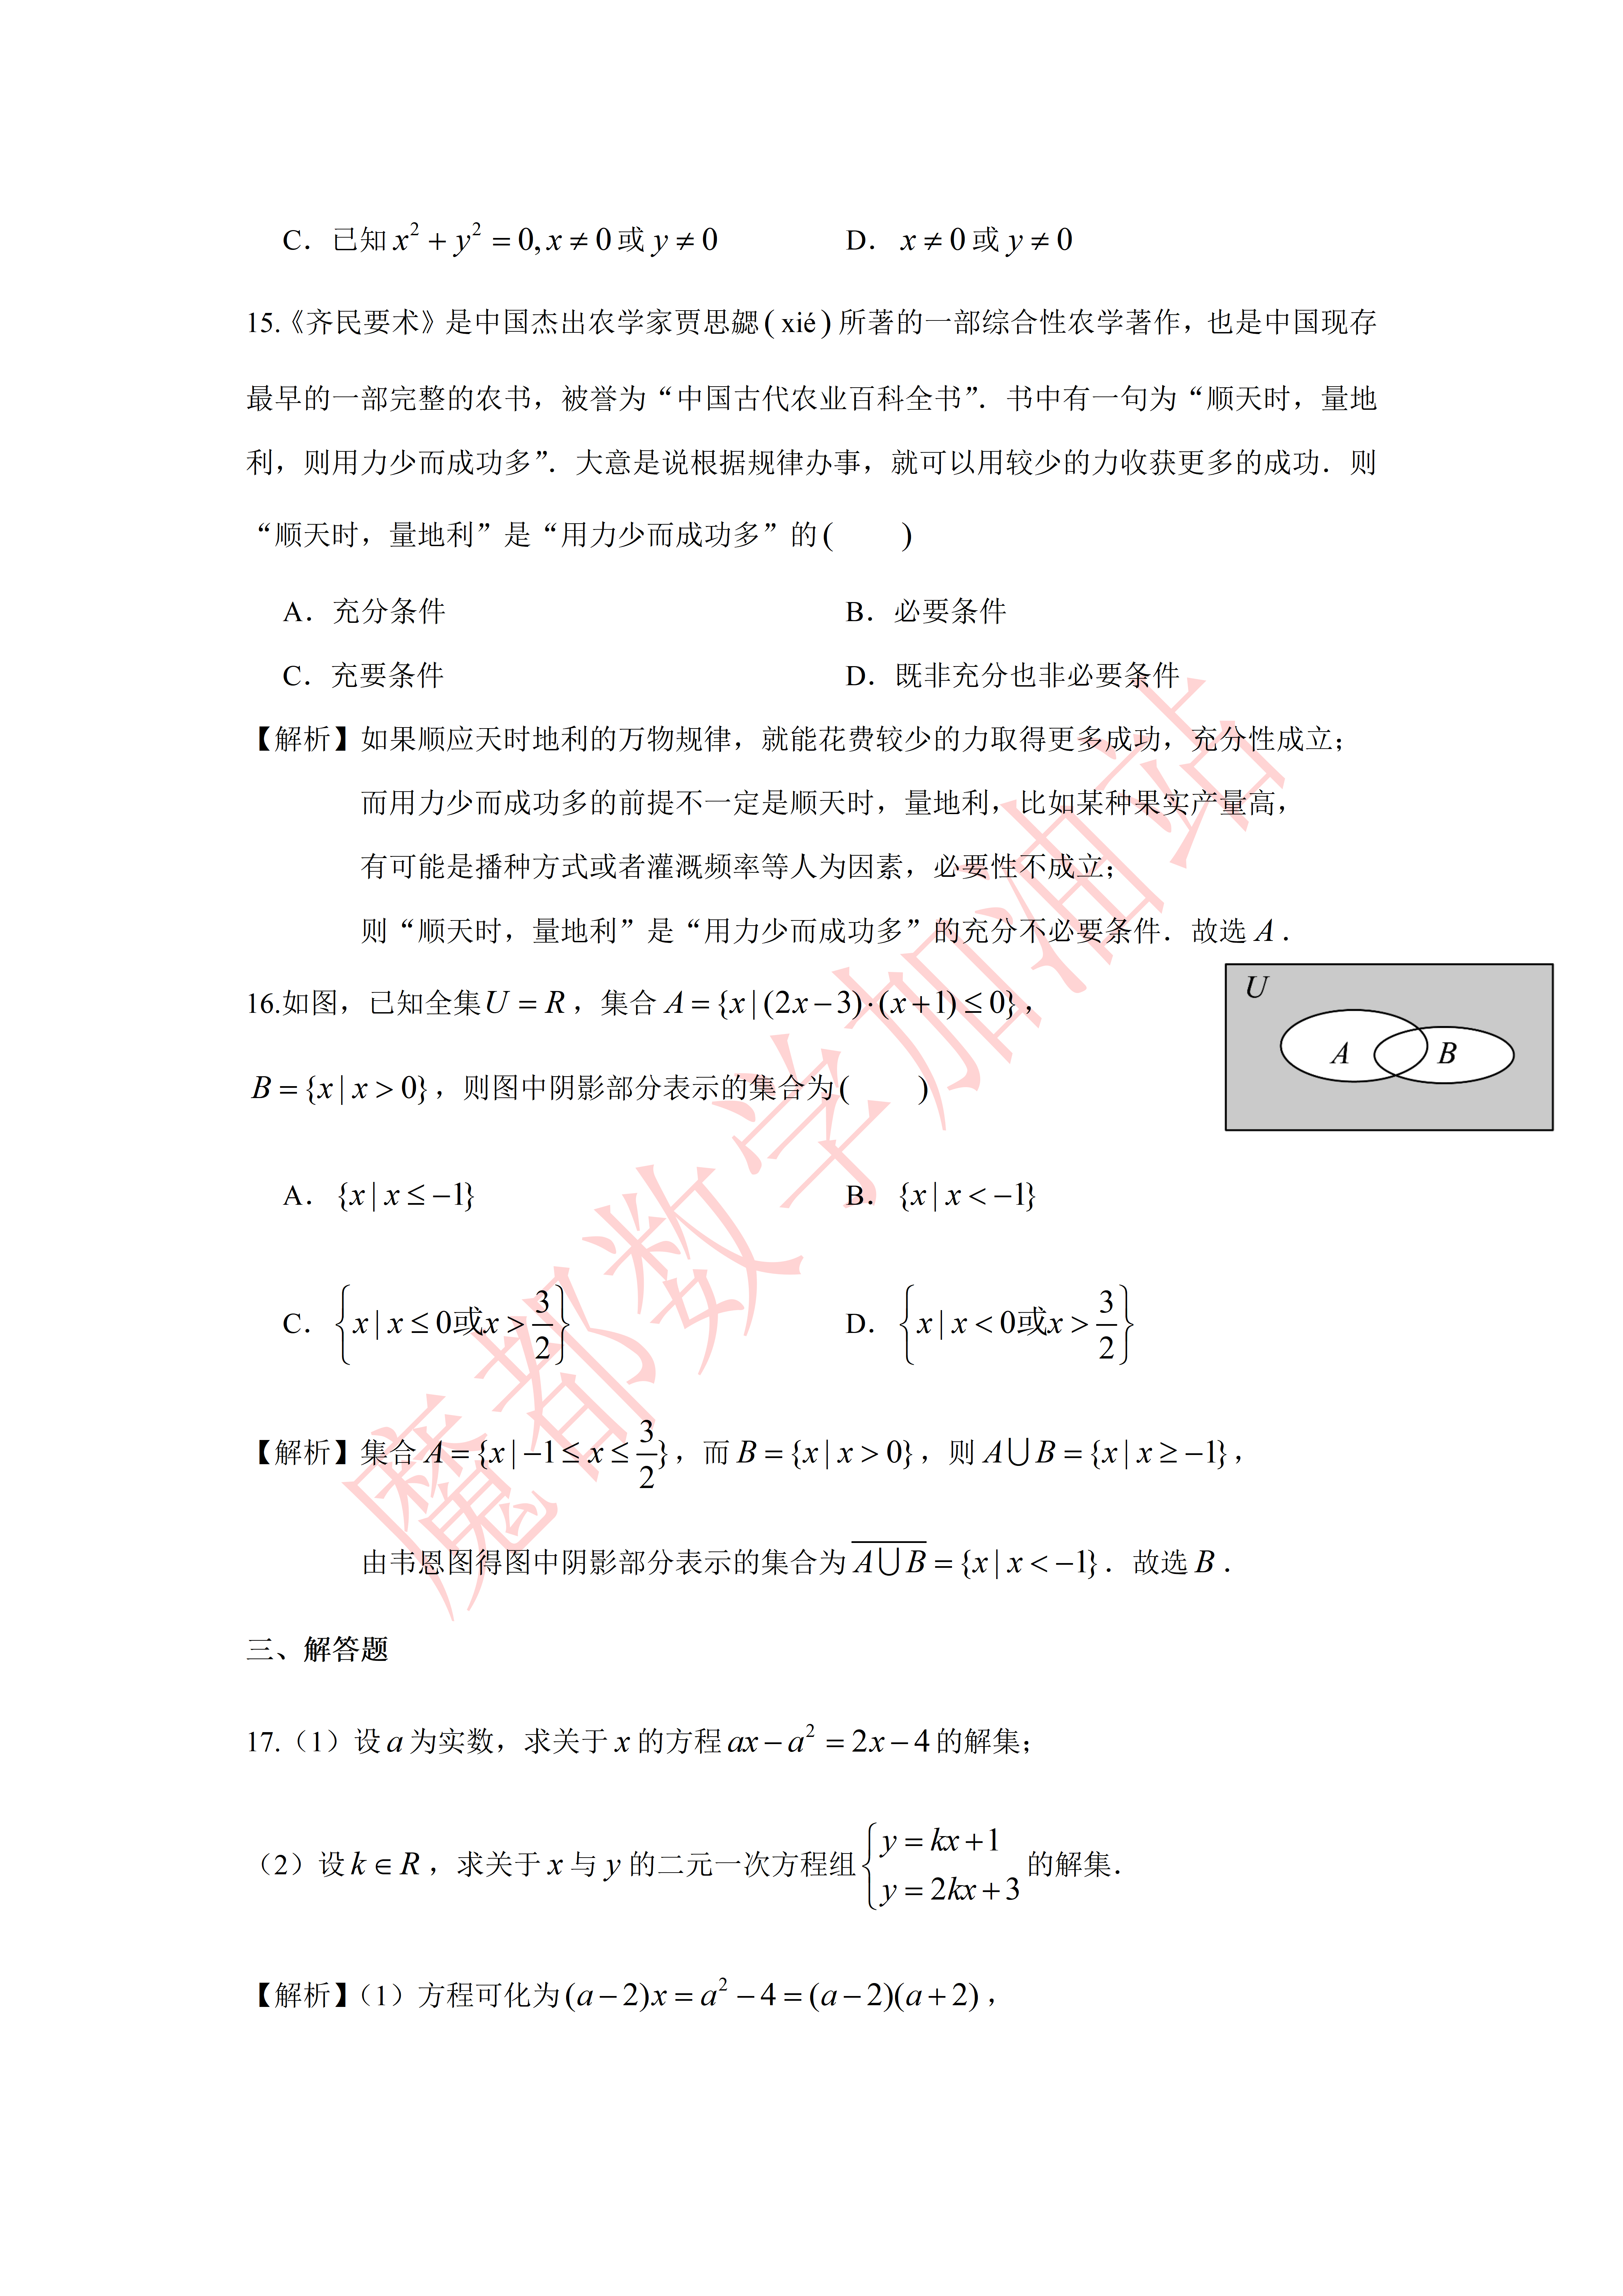
\includegraphics[width=.34\linewidth,trim=3586bp 3410bp 196bp 2818bp,clip]{../原图/高一52_回民中学_9月月考/04.png}
\end{center}

\keepwithprev
A. $\{x\mid x\leqslant-1\}$\qquad B. $\{x\mid x<-1\}$

C. $\left\{x\mid x\leqslant0\text{ 或 }x>\dfrac32\right\}$\qquad D. $\left\{x\mid x<0\text{ 或 }x>\dfrac32\right\}$

\ifanswer
\solbegin
\step{集合 $A=\left\{x\mid-1\leqslant x\leqslant\dfrac32\right\}$，而 $B=\{x\mid x>0\}$，则 $A\cup B=\{x\mid x\geqslant-1\}$，}
\step{由韦恩图得图中阴影部分表示的集合为 $\overline{A\cup B}=\{x\mid x<-1\}$．故选 $B$．}
\solend
\fi

\end{enumerate}

\bigsec{三、解答题}

\begin{enumerate}
\setcounter{enumi}{16}

\item （1）设 $a$ 为实数，求关于 $x$ 的方程 $ax-a^2=2x-4$ 的解集；

（2）设 $k\in\R$，求关于 $x$ 与 $y$ 的二元一次方程组 $\begin{cases}y=kx+1\\y=2kx+3\end{cases}$ 的解集．

\ifanswer
\solbegin
\stepm{(1)}{方程可化为 $(a-2)x=a^2-4=(a-2)(a+2)$，}
\step{当 $a\neq2$ 时，方程的解为 $x=\dfrac{(a-2)(a+2)}{a-2}=a+2$，则解集为 $\{a+2\}$；}
\step{当 $a=2$ 时，方程为 $2x-4=2x-4$，对 $x$ 取一切实数均成立，}
\step{所以解集为 $\R$；}
\stepm{(2)}{$\begin{cases}y=kx+1\\y=2kx+3\end{cases}$，则 $kx+1=2kx+3,kx=-2$，}
\step{当 $k=0$ 时，等式不成立，无解；当 $k\neq0$ 时，$x=-\dfrac2k,y=-1$；}
\step{综上所述，当 $k=0$ 时，解集为 $\varnothing$；当 $k\neq0$ 时，解集为 $\left\{\left(-\dfrac2k,-1\right)\right\}$．}
\solend
\fi

\ansspace[6]

\item 已知命题 $p$：方程 $x^2+6x+m-1=0$ 有两个不等的负根；命题 $q$：方程 $9x^2+6x+m-2=0$ 无实根．

\begin{enumerate}[label=(\arabic*)]
\item 若 $p$ 为真命题，求实数 $m$ 的取值范围；
\item 若 $p,q$ 两命题一真一假，求实数 $m$ 的取值范围．
\end{enumerate}

\ifanswer
\solbegin
\stepm{(1)}{设方程 $x^2+6x+m-1=0$ 两根为 $x_1,x_2$，}
\step{则 $\begin{cases}\Delta>0\\ x_1+x_2<0\\ x_1x_2>0\end{cases}\Rightarrow\begin{cases}36-4(m-1)>0\\ -6<0\\ m-1>0\end{cases}\Rightarrow1<m<10$；}
\stepm{(2)}{若命题 $q$ 为真命题，则 $36-36(m-2)<0\Rightarrow m>3$，}
\step{从而当命题 $q$ 为假命题时，$m\leqslant3$；}
\step{又由（1）得 $p$ 为假命题时，$m\leqslant1$ 或 $m\geqslant10$；}
\step{则当 $p$ 为真命题，$q$ 为假命题时，得 $\begin{cases}1<m<10\\ m\leqslant3\end{cases}\Rightarrow1<m\leqslant3$；}
\step{当 $q$ 为真命题，$p$ 为假命题时，得 $\begin{cases}m\leqslant1\text{ 或 }m\geqslant10\\ m>3\end{cases}\Rightarrow m\geqslant10$；}
\step{综上，当 $p,q$ 两命题一真一假时，$1<m\leqslant3$ 或 $m\geqslant10$.}
\solend
\fi

\ansspace[6]

\item 证明下列两个命题：

\begin{enumerate}[label=(\arabic*)]
\item 设 $ab>0$，求证：$a>b$ 是 $\dfrac1a<\dfrac1b$ 的充要条件．
\item 已知 $a,b$ 为正数，$n$ 为正整数，求证：如果 $a^n>b^n$，那么 $a>b$．
\end{enumerate}

\ifanswer
\solbegin
\stepm{(1)}{先证充分性：因为 $ab>0$ 且 $a>b$，故 $a-b>0$，从而 $\dfrac{a-b}{ab}>0$，}
\step{即 $\dfrac1b-\dfrac1a>0$，即 $\dfrac1a<\dfrac1b$；}
\step{再证必要性：若 $\dfrac1a<\dfrac1b$，则 $\dfrac1a-\dfrac1b=\dfrac{b-a}{ab}<0$，}
\step{又因为 $ab>0$，所以 $b-a<0$，即 $a>b$．}
% 原卷如此，照录未改（第 19 题(1)此句末用全角句号“。”，全卷其余各题末句用“．”，
% 见文件头“原卷笔误/存疑”第 4 条）
\step{综上，$a>b$ 是 $\dfrac1a<\dfrac1b$ 的充要条件。}
\stepm{(2)}{令 $f(x)=x^n,n\in\N^*$，则由幂函数的性质得 $f(x)$ 在第一象限是严格增的，}
\step{而 $a^n>b^n$ 即意味着 $f(a)>f(b)$，且 $a,b$ 为正数，从而 $a>b$．}
\solend
\fi

\ansspace[8]

\item （1）求关于 $x$ 的不等式 $(m-2)x>1-m$ 的解集；

（2）求关于 $x$ 的不等式 $x^2-(a+1)x+a\leqslant0$ 的解集．

\ifanswer
\solbegin
\stepm{(1)}{由不等式 $(m-2)x>1-m$，}
\step{当 $m-2>0$ 时，即 $m>2$ 时，解得 $x>\dfrac{1-m}{m-2}$，}
\step{所以不等式的解集为 $\left(\dfrac{1-m}{m-2},+\infty\right)$；}
\step{当 $m-2=0$ 时，即 $m=2$ 时，不等式即为 $0>-1$ 恒成立，}
\step{即不等式的解集为 $\R$；}
\step{当 $m-2<0$ 时，即 $m<2$ 时，解得 $x<\dfrac{1-m}{m-2}$，}
\step{所以不等式的解集为 $\left(-\infty,\dfrac{1-m}{m-2}\right)$；}
\step{综上，当 $m>2$ 时，解集为 $\left(\dfrac{1-m}{m-2},+\infty\right)$；}
\step{当 $m=2$ 时，解集为 $\R$；}
\step{当 $m<2$ 时，解集为 $\left(-\infty,\dfrac{1-m}{m-2}\right)$．}
\stepm{(2)}{由不等式 $x^2-(a+1)x+a\leqslant0$，可化为 $(x-a)(x-1)\leqslant0$，}
\step{当 $a>1$ 时，解得 $1\leqslant x\leqslant a$，即不等式的解集为 $[1,a]$；}
\step{当 $a=1$ 时，不等式即为 $(x-1)^2\leqslant0$，解得 $x=1$，即不等式的解集为 $\{1\}$；}
\step{当 $a<1$ 时，解得 $a\leqslant x\leqslant1$，即不等式的解集为 $[a,1]$，}
\step{综上，当 $a>1$ 时，解集为 $[1,a]$；}
\step{当 $a=1$ 时，解集为 $\{1\}$；}
\step{当 $a<1$ 时，解集为 $[a,1]$．}
\solend
\fi

\ansspace[10]

\item 已知集合 $A=\{x\mid(x+2)(5-x)\geqslant0\}$，若集合 $B$ 满足 $A\cap B=\varnothing,A\cup B=[-2,7)$．

\begin{enumerate}[label=(\arabic*)]
\item 用区间表示集合 $B$；
\item 若集合 $B$ 是不等式 $-x^2+bx+c>0$ 的解集，求实数 $b,c$ 的值；
\item 已知全集为 $\R$，若关于 $x$ 的不等式 $-1<x-a\leqslant2$ 的解集为 $M$，且“$x\in\overline A$”是“$x\in M$”的必要非充分条件，求实数 $a$ 的取值范围．
\end{enumerate}

\ifanswer
\solbegin
\stepm{(1)}{由题意得 $(x+2)(5-x)\geqslant0\Leftrightarrow(x+2)(x-5)\leqslant0\Rightarrow-2\leqslant x\leqslant5$，}
\step{则 $A=[-2,5]$，又 $A\cap B=\varnothing,A\cup B=[-2,7)$，则 $B=(5,7)$；}
\stepm{(2)}{$-x^2+bx+c>0\Leftrightarrow x^2-bx-c<0$，则 $x^2-bx-c=0$ 两根为 $5,7$，}
\step{则由韦达定理得 $b=12,-c=35\Rightarrow c=-35$；}
\stepm{(3)}{由题意得 $M=(a-1,a+2],\overline A=(-\infty,-2)\cup(5,+\infty)$，}
\step{且“$x\in\overline A$”是“$x\in M$”的必要非充分条件，则 $M$ 是 $\overline A$ 的真子集，}
\step{从而 $a+2<-2$ 或 $a-1\geqslant5$，解得 $a<-4$ 或 $a\geqslant6$，}
\step{所以实数 $a$ 的取值范围为 $(-\infty,-4)\cup[6,+\infty)$．}
\solend
\fi

\ansspace*[10]

\end{enumerate}

\end{document}
"
%
% 原始材料：微信公众号“魔都数学加油站”文章，作者破晓，连载“27学年高一52”；
% 原文标题“27学年高一52——2026-2027年上海市回民中学高一上9月月考”；
% 原文链接：https://mp.weixin.qq.com/s/ndjyozrRQCLl4ba3J8uR7g。
% 该页面用 JS 渲染，未见明确发布日期；页面内时间戳约为 2026-10-06 21:19／21:38，本稿以该时刻记可得日期。
% 正文为 8 张 PNG 页：第 01—07 页 4762×6735，第 08 页 2560×3620（**同一篇各页分辨率不同**），
% 均按页序读取。8 页全为试卷正文页（卷首标题在第 1 页页顶，卷末解答题第 21 题解析止于第 8 页），
% 无封面页、目录页、二维码或宣传页。粉色斜排“魔都数学加油站”为卷面水印，与公众号页脚一并未录入。
%
% 卷首标题：照卷面印作“2026--2027 年回民中学高一上 9 月月考”（公众号标题中的“上海市”
% 卷面标题行没有，本稿照卷面），年份区间按全稿惯例排 en dash。原卷只有一行标题、无副标题。
%
% 篇幅与题号：原卷自第 3 题起编号（第 1、2 题不在本卷内）。填空题 3—12（10 题）、
% 选择题 13—16（4 题）、解答题 17—21（5 题），共 19 题。本稿沿用原节与原题号，
% 只改排为全稿统一的大节样式（原卷小节标题为“一、填空题”“二、选择题”“三、解答题”）。
%
% 讲评版：原卷每题下直接印【答案】或【解析】。**只印【答案】的 1 题**（第 3 题），本稿只给 \ans{}；
% **第 14 题没有任何【答案】/【解析】段**，答案“D”直接印在题干括号内（“应假设(  D  )”），
% 本稿按 高一37 第 13 题的成例把括号留空、答案另提为 \ans{$D$}；
% 其余 17 题都只印【解析】，按全稿口径这类题不另提 \ans{}——其中选择题第 13、15、16 题的结论
% 写在解析末句（“故选 A／A／B”），亦照录在解析内。
%
% 副标题：原卷未印副标题。本稿按“知识模块”口径标作“集合与常用逻辑用语、不等式”：
% 19 题中集合与常用逻辑用语 10 题（集合类 7 题——第 3、4、5、9、12、16、21 题；
% 逻辑类 3 题——第 6、14、15 题），不等式 9 题（含等式性质与一元二次方程：第 7、8、10、11、
% 13、17、18、19、20 题），两类均远超三分之一，故并标。口径同 高一46、高一47、高一48、高一51。
%
% 与原卷的排版差异：
%   ① 原卷每题下直接印【答案】/【解析】，本稿按全稿惯例将答案与解析置于答案版，试卷版保持干净；
%      第 14 题印在题干括号内的答案“D”同样移入 \ans{}，见上；
%   ② 原卷未印副标题，本稿按“知识模块”口径补出；
%   ③ 原卷填空横线约两个字宽，本稿按全稿惯例统一排 \blankline[4.4em]；
%      选择题的作答括号原卷排半角“(    )”，本稿按全稿惯例排 \mbox{（\quad）}；
%   ④ 原卷实数集、自然数集排斜体/粗体 $R$、$\mathbf{R}$、$N$，本稿按全稿惯例改用 $\R$、$\N$；
%      空集记号统一为 \varnothing；
%   ⑤ 第 8 题题干与解析两处“两个实数分别为 $x_1$、$x_2$”原卷即用顿号，第 10、13 题等处
%      原卷在数学式内用半角逗号（如 $x_1,x_2$、$a,b,c\in R$），两份均照录未强改；
%      句末句点按全稿惯例排西文句点，句中句点（第 9、12、15、21 题）照原卷排全角“．”；
%   ⑥ 第 17、20 题原卷把子问标号“（1）”排在该题题号同一行，本稿照原卷仍排同一行（同 高一34 的
%      做法）；第 18、19、21 题的子问原卷各自另起一行，本稿按全稿惯例用 enumerate 的 (1)(2)(3)；
%      解析中的子问标号一律用 \stepm{(1)}{…}；
%   ⑦ 第 16 题的韦恩图原卷排在题干与选项右侧的浮动位置，本稿居中排在题干之后、选项之前，
%      并加 \needvspace 整块推走（守卫写在 \item 之前）；图自原图第 4 页裁切（trim），不另存图片文件；
%   ⑧ 每道解答题原卷未留作答空白，本稿按全稿惯例加 \ansspace。
%
% 原卷笔误/存疑（均照录未改，正文对应处另有 % 注）：
%   1. 第 8 题题干与解析首行两处均作“两个实数分别为 $x_1$、$x_2$”，按文意应为“两个实数**根**”
%      （疑脱“根”字，第 10 题同位置作“两个实根分别是”）；
%   2. 第 4 题解析“满足条件的 $A$ 的个数为集合 $\{0,1,3\}$ 的真子集，即 7 个”，
%      “个数为……真子集”表述不严（应为“……的真子集的个数”）；$\{0,1,3\}$ 的真子集 7 个，结论无误；
%   3. 第 6 题解析第 2 行“当 $a=10,b=0.2$ 时，$a+b>2$，且 $ab>1$，所以 $a>1$，且 $b>1$ 不成立”
%      ——此处是举反例，“所以”按文意应为“但”（$a=10,b=0.2$ 与“$a>1$ 且 $b>1$”不成立之间是转折，
%      非因果）；
%   4. 第 19 题 (1) 解析末行“综上，$a>b$ 是 $\dfrac1a<\dfrac1b$ 的充要条件。”用全角句号“。”，
%      全卷其余各题末句均用“．”，体例不一，照录；
%   5. 第 20 题第 (1) 问解析先按 $m>2$、$m=2$、$m<2$ 三种情况各给出解集，末三行又“综上”重述一遍，
%      与原卷一致（内容重复，非笔误）；
%   6. 第 18 题题干第 (2) 问“若 $p,q$ 两命题一真一假”，正文照录原卷所用半角逗号（未改顿号）。
%
% 插图：1 张，自原图裁切（无 \begin{tikzpicture} 重排）：
%   · 第 16 题题干韦恩图（全集 $U$ 矩形内两相交椭圆 $A$、$B$，灰色为阴影部分）
%     ——原图第 04 页，原卷排于题干与选项右侧。
%     裁框：x 3594–4558、y 2826–3317（即矩形外框，四周各留 4px），
%     trim=3590bp 3414bp 200bp 2822bp（左／下／右／上），页宽 4762、页高 6735。
%
\documentclass[a4paper,11pt]{article}
\usepackage{common}

\begin{document}

\examtitlest[3]{2026--2027 年回民中学高一上 9 月月考}{集合与常用逻辑用语、不等式}

\bigsec{一、填空题}

\begin{enumerate}
\setcounter{enumi}{2}

\item 用列举法写出下列集合 $\{(x,y)\mid x+y=2,x\in\N,y\in\N\}=$\blankline[4.4em].

\ifanswer
\ans{$\{(0,2),(1,1),(2,0)\}$}
\fi

\item 设集合 $A$ 满足 $\{-1,2\}\sub A\subset\{-1,0,1,2,3\}$，则满足条件的 $A$ 有\blankline[4.4em]个.

\ifanswer
\solbegin
\step{满足条件的 $A$ 的个数为集合 $\{0,1,3\}$ 的真子集，即 $7$ 个.}
\solend
\fi

\item 已知集合 $A=\{2,(a+1)^2,a^2+2\}$，且 $1\in A$，则实数 $a$ 的值为\blankline[4.4em].

\ifanswer
\solbegin
\step{因为 $1\in A$，而 $a^2+2\geqslant2$，所以 $(a+1)^2=1$，解得 $a=0$ 或 $a=-2$，}
\step{$a=0$ 时，$a^2+2=2$，不合题意，$a=-2$ 时，$a^2+2=6$，满足题意，}
\step{所以 $a=-2$.}
\solend
\fi

\item 已知 $a,b$ 是实数，则“$a>1$，且 $b>1$”是“$a+b>2$，且 $ab>1$”的\blankline[4.4em]条件.

\ifanswer
\solbegin
\step{$a,b$ 是实数，则“$a>1$，且 $b>1$”$\Rightarrow$“$a+b>2$，且 $ab>1$”正确，}
% 原卷如此，照录未改（第 6 题解析此处作“所以 $a>1$，且 $b>1$ 不成立”，按文意为转折，
% 见文件头“原卷笔误/存疑”第 3 条）
\step{当 $a=10,b=0.2$ 时，$a+b>2$，且 $ab>1$，所以 $a>1$，且 $b>1$ 不成立，}
\step{即前者是推出后者，后者推不出前者，}
\step{所以“$a>1$，且 $b>1$”是“$a+b>2$，且 $ab>1$”的充分而不必要条件.}
\solend
\fi

\item 已知等式 $2x^2-3x-1=a(x-1)^2+b(x-1)+c$ 恒成立，其中 $a,b,c$ 为常数，则 $a+b-c=$\blankline[4.4em].

\ifanswer
\solbegin
\step{将等式右侧展开整理得 $a(x-1)^2+b(x-1)+c=ax^2+(-2a+b)x+(a-b+c)$，}
\step{左右两边多项式恒等，对应次数的系数必须相等：}
\step{则 $a=2,-2a+b=-3$，代入 $a=2$ 得 $b=1$，$a-b+c=-1$，}
\step{代入 $a=2,b=1$ 得 $c=-2$，得 $a+b-c=2+1-(-2)=5$.}
\solend
\fi

% 原卷如此，照录未改（第 8 题题干与解析首行两处“两个实数分别为”疑脱“根”字，
% 见文件头“原卷笔误/存疑”第 1 条）
\item 若关于 $x$ 的二次方程 $x^2+mx+4m^2-3=0$ 的两个实数分别为 $x_1$、$x_2$，且满足 $x_1+x_2=x_1x_2$，则实数 $m$ 的值为\blankline[4.4em].

\ifanswer
\solbegin
% 原卷如此，照录未改（此处“两个实数分别为”同题干，疑脱“根”字）
\step{二次方程 $x^2+mx+4m^2-3=0$ 的两个实数分别为 $x_1$、$x_2$，}
\step{则有 $\Delta=m^2-4(4m^2-3)\geqslant0$，变形得 $m^2\leqslant\dfrac45$，}
\step{则 $x_1+x_2=-m$，$x_1x_2=(4m^2-3)$，}
\step{若 $x_1+x_2=x_1x_2$，则有 $-m=4m^2-3$，解得 $m=-1$ 或 $\dfrac34$，}
\step{又 $m^2\leqslant\dfrac45$，则 $m=\dfrac34$.}
\solend
\fi

\item 设集合 $A=\{x\mid x^2=1\}$，$B=\{x\mid ax=1\}$．若 $A\cap B=B$，则实数 $a$ 的值为\blankline[4.4em].

\ifanswer
\solbegin
\step{集合 $A=\{x\mid x^2=1\}=\{-1,1\}$，$B=\{x\mid ax=1\}$，$A\cap B=B$，所以 $B\sub A$，}
\step{当 $a=0$ 时，$B=\varnothing$，成立；}
\step{当 $a\neq0$ 时，$B=\left\{\dfrac1a\right\}$，则 $\dfrac1a=-1$ 或 $\dfrac1a=1$，解得 $a=-1$ 或 $a=1$，}
\step{所以实数 $a$ 的值为 $0$ 或 $1$ 或 $-1$.}
\solend
\fi

\item 已知关于 $x$ 的一元二次方程 $x^2+3x-3=0$ 的两个实根分别是 $x_1,x_2$，则以 $-\dfrac1{x_1},-\dfrac1{x_2}$ 为根且二次项系数是 $1$ 的一元二次方程为\blankline[4.4em].

\ifanswer
\solbegin
\step{因为 $x_1,x_2$ 是一元二次方程 $x^2+3x-3=0$ 的两个实根，}
\step{所以 $x_1+x_2=-3,x_1x_2=-3$，}
\step{所以 $-\dfrac1{x_1}+\left(-\dfrac1{x_2}\right)=-\dfrac{x_1+x_2}{x_1x_2}=-1$，$-\dfrac1{x_1}\cdot\left(-\dfrac1{x_2}\right)=\dfrac1{x_1x_2}=-\dfrac13$，}
\step{所以一元二次方程为 $x^2+x-\dfrac13=0$.}
\solend
\fi

\item 若关于 $x$ 的不等式 $(a-2)x^2+2(a-2)x-4<0$ 的解集是 $\R$，则实数 $a$ 的取值范围是\blankline[4.4em].

\ifanswer
\solbegin
\step{当 $a=2$ 时，不等式化为 $-4<0$ 对于任意实数 $x$ 都成立，因此 $a=2$ 满足题意；}
\step{当 $a\neq2$ 时，要使关于 $x$ 的不等式 $(a-2)x^2+2(a-2)x-4<0$ 的解集为 $\R$，}
\step{则 $\begin{cases}a-2<0\\ \Delta=4(a-2)^2+16(a-2)<0\end{cases}$，解得 $-2<a<2$．}
\step{综上，$a$ 的取值范围为 $(-2,2]$．}
\solend
\fi

\item 设非空集合 $A$、$B$，定义 $A\times B=\{x\mid x\in(A\cup B),x\notin(A\cap B)\}$．已知 $A=\{x\mid0\leqslant x\leqslant2\}$，$B=\{y\mid y\geqslant0\}$，则 $A\times B=$\blankline[4.4em].

\ifanswer
\solbegin
\step{由于 $A=\{x\mid0\leqslant x\leqslant2\}$，$B=\{y\mid y\geqslant0\}=\{x\mid x\geqslant0\}$，}
\step{所以 $A\cup B=\{x\mid x\geqslant0\}$，$A\cap B=\{x\mid0\leqslant x\leqslant2\}$，故 $A\times B=\{x\mid x>2\}$．}
\solend
\fi

\end{enumerate}

\bigsec{二、选择题}

\begin{enumerate}
\setcounter{enumi}{12}

\item 已知 $a,b,c\in\R$ 且 $a>b$，则下列不等式一定成立的是\mbox{（\quad）}

\keepwithprev
A. $\dfrac{a}{c^2+1}>\dfrac{b}{c^2+1}$\qquad B. $\dfrac1a<\dfrac1b$

C. $ac>bc$\qquad D. $a^2>b^2$

\ifanswer
\solbegin
\step{对于 A：因为 $c^2+1>0$ 恒成立，且 $a>b$，所以 $\dfrac{a}{c^2+1}>\dfrac{b}{c^2+1}$ 一定成立，}
\step{所以 A 正确；}
\step{对于 B：当 $a=1,b=-1$ 时，满足 $a>b$，此时 $\dfrac1a=1>\dfrac1b=-1$，所以 B 错误；}
\step{对于 C：当 $c<0$ 时，由 $a>b$，得 $ac<bc$，所以 C 错误；}
\step{对于 D：当 $a=1,b=-2$ 时，满足 $a>b$，此时 $a^2=1<b^2=4$，所以 D 错误；}
\step{故选 $A$．}
\solend
\fi

% 注：本题的答案“D”原卷直接印在题干末尾的括号内（“应假设(  D  )”），且没有单独的
%     【答案】/【解析】段，本稿按 高一37 第 13 题的成例把括号留空、另提为 \ans{}，
%     见文件头“与原卷的排版差异”①。
\item 用反证法证明：“已知 $x,y\in\R$,$x^2+y^2=0$，求证：$x=y=0$”时，应假设\mbox{（\quad）}

\keepwithprev
A. 已知 $x^2+y^2=0,x\neq0$ 且 $y\neq0$\qquad B. $x\neq0$ 且 $y\neq0$

C. 已知 $x^2+y^2=0,x\neq0$ 或 $y\neq0$\qquad D. $x\neq0$ 或 $y\neq0$

\ans{$D$}

\item 《齐民要术》是中国杰出农学家贾思勰（xié）所著的一部综合性农学著作，也是中国现存最早的一部完整的农书，被誉为“中国古代农业百科全书”．书中有一句为“顺天时，量地利，则用力少而成功多”．大意是说根据规律办事，就可以用较少的力收获更多的成功．则“顺天时，量地利”是“用力少而成功多”的\mbox{（\quad）}

\keepwithprev
A. 充分条件\qquad B. 必要条件

C. 充要条件\qquad D. 既非充分也非必要条件

\ifanswer
\solbegin
\step{如果顺应天时地利的万物规律，就能花费较少的力取得更多成功，充分性成立；}
\step{而用力少而成功多的前提不一定是顺天时，量地利，比如某种果实产量高，}
\step{有可能是播种方式或者灌溉频率等人为因素，必要性不成立；}
\step{则“顺天时，量地利”是“用力少而成功多”的充分不必要条件．故选 $A$．}
\solend
\fi

\needvspace{13\baselineskip}

\item 如图，已知全集 $U=\R$，集合 $A=\{x\mid(2x-3)\cdot(x+1)\leqslant0\}$，$B=\{x\mid x>0\}$，则图中阴影部分表示的集合为\mbox{（\quad）}

\begin{center}
% 原图第 4 页题干韦恩图直接裁取（原卷排于题干与选项右侧）。
% 裁框取矩形外框 x 3590–4558、y 2822–3321，再向外各留 4px（即 x 3586–4562、y 2818–3325），
% trim=左 3586bp／下 3410bp／右 196bp／上 2818bp（页宽 4762、页高 6735）。
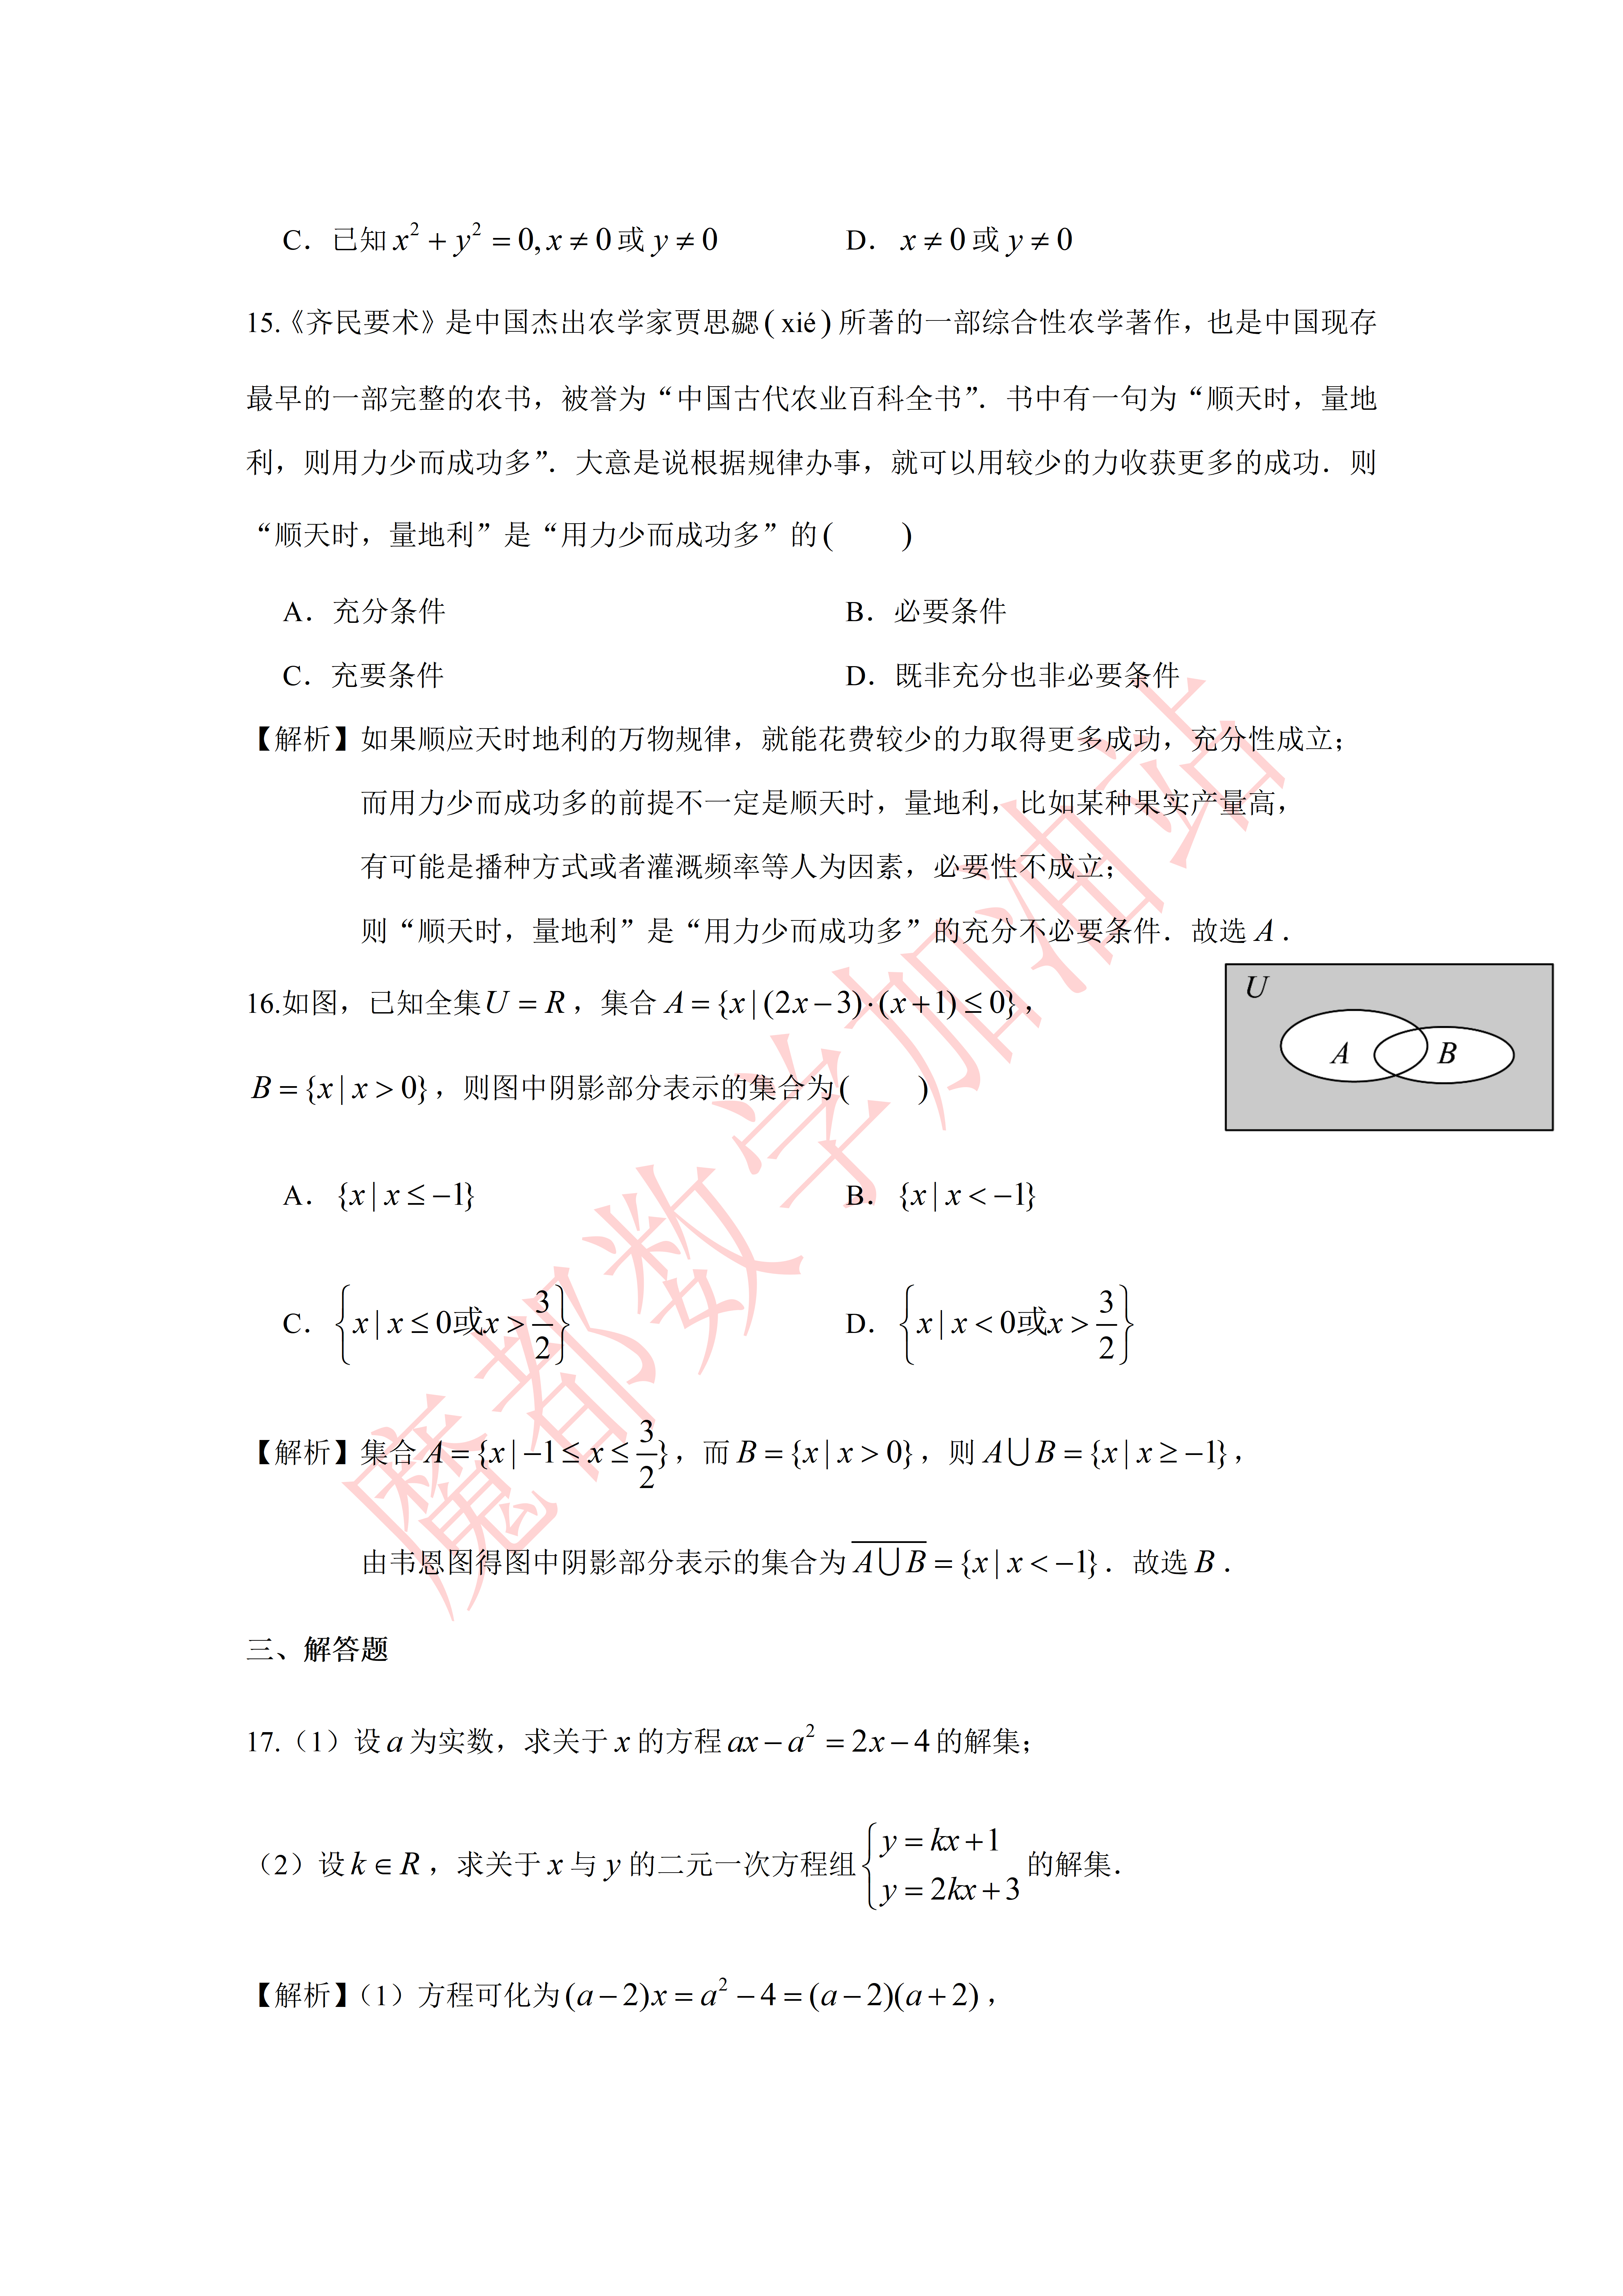
\includegraphics[width=.34\linewidth,trim=3586bp 3410bp 196bp 2818bp,clip]{../原图/高一52_回民中学_9月月考/04.png}
\end{center}

\keepwithprev
A. $\{x\mid x\leqslant-1\}$\qquad B. $\{x\mid x<-1\}$

C. $\left\{x\mid x\leqslant0\text{ 或 }x>\dfrac32\right\}$\qquad D. $\left\{x\mid x<0\text{ 或 }x>\dfrac32\right\}$

\ifanswer
\solbegin
\step{集合 $A=\left\{x\mid-1\leqslant x\leqslant\dfrac32\right\}$，而 $B=\{x\mid x>0\}$，则 $A\cup B=\{x\mid x\geqslant-1\}$，}
\step{由韦恩图得图中阴影部分表示的集合为 $\overline{A\cup B}=\{x\mid x<-1\}$．故选 $B$．}
\solend
\fi

\end{enumerate}

\bigsec{三、解答题}

\begin{enumerate}
\setcounter{enumi}{16}

\item （1）设 $a$ 为实数，求关于 $x$ 的方程 $ax-a^2=2x-4$ 的解集；

（2）设 $k\in\R$，求关于 $x$ 与 $y$ 的二元一次方程组 $\begin{cases}y=kx+1\\y=2kx+3\end{cases}$ 的解集．

\ifanswer
\solbegin
\stepm{(1)}{方程可化为 $(a-2)x=a^2-4=(a-2)(a+2)$，}
\step{当 $a\neq2$ 时，方程的解为 $x=\dfrac{(a-2)(a+2)}{a-2}=a+2$，则解集为 $\{a+2\}$；}
\step{当 $a=2$ 时，方程为 $2x-4=2x-4$，对 $x$ 取一切实数均成立，}
\step{所以解集为 $\R$；}
\stepm{(2)}{$\begin{cases}y=kx+1\\y=2kx+3\end{cases}$，则 $kx+1=2kx+3,kx=-2$，}
\step{当 $k=0$ 时，等式不成立，无解；当 $k\neq0$ 时，$x=-\dfrac2k,y=-1$；}
\step{综上所述，当 $k=0$ 时，解集为 $\varnothing$；当 $k\neq0$ 时，解集为 $\left\{\left(-\dfrac2k,-1\right)\right\}$．}
\solend
\fi

\ansspace[6]

\item 已知命题 $p$：方程 $x^2+6x+m-1=0$ 有两个不等的负根；命题 $q$：方程 $9x^2+6x+m-2=0$ 无实根．

\begin{enumerate}[label=(\arabic*)]
\item 若 $p$ 为真命题，求实数 $m$ 的取值范围；
\item 若 $p,q$ 两命题一真一假，求实数 $m$ 的取值范围．
\end{enumerate}

\ifanswer
\solbegin
\stepm{(1)}{设方程 $x^2+6x+m-1=0$ 两根为 $x_1,x_2$，}
\step{则 $\begin{cases}\Delta>0\\ x_1+x_2<0\\ x_1x_2>0\end{cases}\Rightarrow\begin{cases}36-4(m-1)>0\\ -6<0\\ m-1>0\end{cases}\Rightarrow1<m<10$；}
\stepm{(2)}{若命题 $q$ 为真命题，则 $36-36(m-2)<0\Rightarrow m>3$，}
\step{从而当命题 $q$ 为假命题时，$m\leqslant3$；}
\step{又由（1）得 $p$ 为假命题时，$m\leqslant1$ 或 $m\geqslant10$；}
\step{则当 $p$ 为真命题，$q$ 为假命题时，得 $\begin{cases}1<m<10\\ m\leqslant3\end{cases}\Rightarrow1<m\leqslant3$；}
\step{当 $q$ 为真命题，$p$ 为假命题时，得 $\begin{cases}m\leqslant1\text{ 或 }m\geqslant10\\ m>3\end{cases}\Rightarrow m\geqslant10$；}
\step{综上，当 $p,q$ 两命题一真一假时，$1<m\leqslant3$ 或 $m\geqslant10$.}
\solend
\fi

\ansspace[6]

\item 证明下列两个命题：

\begin{enumerate}[label=(\arabic*)]
\item 设 $ab>0$，求证：$a>b$ 是 $\dfrac1a<\dfrac1b$ 的充要条件．
\item 已知 $a,b$ 为正数，$n$ 为正整数，求证：如果 $a^n>b^n$，那么 $a>b$．
\end{enumerate}

\ifanswer
\solbegin
\stepm{(1)}{先证充分性：因为 $ab>0$ 且 $a>b$，故 $a-b>0$，从而 $\dfrac{a-b}{ab}>0$，}
\step{即 $\dfrac1b-\dfrac1a>0$，即 $\dfrac1a<\dfrac1b$；}
\step{再证必要性：若 $\dfrac1a<\dfrac1b$，则 $\dfrac1a-\dfrac1b=\dfrac{b-a}{ab}<0$，}
\step{又因为 $ab>0$，所以 $b-a<0$，即 $a>b$．}
% 原卷如此，照录未改（第 19 题(1)此句末用全角句号“。”，全卷其余各题末句用“．”，
% 见文件头“原卷笔误/存疑”第 4 条）
\step{综上，$a>b$ 是 $\dfrac1a<\dfrac1b$ 的充要条件。}
\stepm{(2)}{令 $f(x)=x^n,n\in\N^*$，则由幂函数的性质得 $f(x)$ 在第一象限是严格增的，}
\step{而 $a^n>b^n$ 即意味着 $f(a)>f(b)$，且 $a,b$ 为正数，从而 $a>b$．}
\solend
\fi

\ansspace[8]

\item （1）求关于 $x$ 的不等式 $(m-2)x>1-m$ 的解集；

（2）求关于 $x$ 的不等式 $x^2-(a+1)x+a\leqslant0$ 的解集．

\ifanswer
\solbegin
\stepm{(1)}{由不等式 $(m-2)x>1-m$，}
\step{当 $m-2>0$ 时，即 $m>2$ 时，解得 $x>\dfrac{1-m}{m-2}$，}
\step{所以不等式的解集为 $\left(\dfrac{1-m}{m-2},+\infty\right)$；}
\step{当 $m-2=0$ 时，即 $m=2$ 时，不等式即为 $0>-1$ 恒成立，}
\step{即不等式的解集为 $\R$；}
\step{当 $m-2<0$ 时，即 $m<2$ 时，解得 $x<\dfrac{1-m}{m-2}$，}
\step{所以不等式的解集为 $\left(-\infty,\dfrac{1-m}{m-2}\right)$；}
\step{综上，当 $m>2$ 时，解集为 $\left(\dfrac{1-m}{m-2},+\infty\right)$；}
\step{当 $m=2$ 时，解集为 $\R$；}
\step{当 $m<2$ 时，解集为 $\left(-\infty,\dfrac{1-m}{m-2}\right)$．}
\stepm{(2)}{由不等式 $x^2-(a+1)x+a\leqslant0$，可化为 $(x-a)(x-1)\leqslant0$，}
\step{当 $a>1$ 时，解得 $1\leqslant x\leqslant a$，即不等式的解集为 $[1,a]$；}
\step{当 $a=1$ 时，不等式即为 $(x-1)^2\leqslant0$，解得 $x=1$，即不等式的解集为 $\{1\}$；}
\step{当 $a<1$ 时，解得 $a\leqslant x\leqslant1$，即不等式的解集为 $[a,1]$，}
\step{综上，当 $a>1$ 时，解集为 $[1,a]$；}
\step{当 $a=1$ 时，解集为 $\{1\}$；}
\step{当 $a<1$ 时，解集为 $[a,1]$．}
\solend
\fi

\ansspace[10]

\item 已知集合 $A=\{x\mid(x+2)(5-x)\geqslant0\}$，若集合 $B$ 满足 $A\cap B=\varnothing,A\cup B=[-2,7)$．

\begin{enumerate}[label=(\arabic*)]
\item 用区间表示集合 $B$；
\item 若集合 $B$ 是不等式 $-x^2+bx+c>0$ 的解集，求实数 $b,c$ 的值；
\item 已知全集为 $\R$，若关于 $x$ 的不等式 $-1<x-a\leqslant2$ 的解集为 $M$，且“$x\in\overline A$”是“$x\in M$”的必要非充分条件，求实数 $a$ 的取值范围．
\end{enumerate}

\ifanswer
\solbegin
\stepm{(1)}{由题意得 $(x+2)(5-x)\geqslant0\Leftrightarrow(x+2)(x-5)\leqslant0\Rightarrow-2\leqslant x\leqslant5$，}
\step{则 $A=[-2,5]$，又 $A\cap B=\varnothing,A\cup B=[-2,7)$，则 $B=(5,7)$；}
\stepm{(2)}{$-x^2+bx+c>0\Leftrightarrow x^2-bx-c<0$，则 $x^2-bx-c=0$ 两根为 $5,7$，}
\step{则由韦达定理得 $b=12,-c=35\Rightarrow c=-35$；}
\stepm{(3)}{由题意得 $M=(a-1,a+2],\overline A=(-\infty,-2)\cup(5,+\infty)$，}
\step{且“$x\in\overline A$”是“$x\in M$”的必要非充分条件，则 $M$ 是 $\overline A$ 的真子集，}
\step{从而 $a+2<-2$ 或 $a-1\geqslant5$，解得 $a<-4$ 或 $a\geqslant6$，}
\step{所以实数 $a$ 的取值范围为 $(-\infty,-4)\cup[6,+\infty)$．}
\solend
\fi

\ansspace*[10]

\end{enumerate}

\end{document}
